\documentclass[a4paper,14pt,oneside,openany]{memoir}

%package
\newif\ifsynopsis           % Условие, проверяющее, что документ --- автореферат

%%%% Проверка используемого TeX-движка %%%
%\RequirePackage{ifxetex, ifluatex}
%\newif\ifxetexorluatex   % определяем новый условный оператор (http://tex.stackexchange.com/a/47579)
%\ifxetex
%    \xetexorluatextrue
%\else
%    \ifluatex
%        \xetexorluatextrue
%    \else
%        \xetexorluatexfalse
%    \fi
%\fi

\newif\ifsynopsis           % Условие, проверяющее, что документ --- автореферат

\RequirePackage{etoolbox}[2015/08/02]               % Для продвинутой проверки разных условий

%%% Поля и разметка страницы %%%
%\usepackage{pdflscape}                              % Для включения альбомных страниц
\usepackage{geometry}                               % Для последующего задания полей

%%% Математические пакеты %%%
\usepackage{amsthm,amsmath,amscd}       % Математические дополнения от AMS
%\ifxetexorluatex
    \usepackage{amsfonts,amssymb}       % Математические дополнения от AMS
%\else
%    \ifnumequal{\value{usealtfont}}{2}{}{
%        \usepackage{amsfonts,amssymb}       % Математические дополнения от AMS
%    }
%\fi

\usepackage{mathtools}                  % Добавляет окружение multlined

%%%% Установки для размера шрифта 14 pt %%%%
%% Формирование переменных и констант для сравнения (один раз для всех подключаемых файлов)%%
%% должно располагаться до вызова пакета fontspec или polyglossia, потому что они сбивают его работу
\newlength{\curtextsize}
\newlength{\bigtextsize}
\setlength{\bigtextsize}{13.9pt}

\makeatletter
%\show\f@size                                       % неплохо для отслеживания, но вызывает стопорение процесса, если документ компилируется без команды  -interaction=nonstopmode
\setlength{\curtextsize}{\f@size pt}
\makeatother

%%% Кодировки и шрифты %%%
%\ifxetexorluatex
%    \usepackage{polyglossia}[2014/05/21]            % Поддержка многоязычности (fontspec подгружается автоматически)
%\else
   %%% Решение проблемы копирования текста в буфер кракозябрами
%    \ifnumequal{\value{usealtfont}}{1}{% Используется pscyr, при наличии
%        \IfFileExists{pscyr.sty}{% вероятно, без pscyr нет необходимости в этом коде
%            \input glyphtounicode.tex
%            \input glyphtounicode-cmr.tex %from pdfx package
%            \pdfgentounicode=1
%        }{}
%    }{}
%    \usepackage{cmap}                               % Улучшенный поиск русских слов в полученном pdf-файле
    \defaulthyphenchar=127                          % Если стоит до fontenc, то переносы не впишутся в выделяемый текст при копировании его в буфер обмена
    \usepackage[T1,T2A]{fontenc}                    % Поддержка русских букв
%    \ifnumequal{\value{usealtfont}}{1}{% Используется pscyr, при наличии
%        \IfFileExists{pscyr.sty}{\usepackage{pscyr}}{}  % Подключение pscyr
%    }{}
%    \usepackage[cp1251]{inputenc}%[2014/04/30]         % Кодировка utf8
   \usepackage[utf8]{inputenc}[2014/04/30]         % Кодировка utf8
    \usepackage[english, russian, ukrainian]{babel}%[2014/03/24]% Языки: русский, английский
%    \usepackage{pscyr}
%    \ifnumequal{\value{usealtfont}}{2}{
%        % http://dxdy.ru/post1238763.html#p1238763
%        \usepackage[scaled=0.925]{XCharter}[2017/06/25] % Подключение русифицированных шрифтов XCharter
%        \usepackage[bitstream-charter]{mathdesign} % Согласование математических шрифтов
%    }{}
%\fi

%%% Оформление абзацев %%%
\usepackage{indentfirst}                            % Красная строка

%%% Цвета %%%
%\usepackage[dvipsnames, table, hyperref, cmyk]{xcolor} % Совместимо с tikz. Конвертация всех цветов в cmyk заложена как удовлетворение возможного требования типографий. Возможно конвертирование и в rgb.
\usepackage{xcolor} % Совместимо с tikz. Конвертация всех цветов в cmyk заложена как удовлетворение возможного требования типографий. Возможно

%%% Таблицы %%%
\usepackage{longtable,ltcaption}                    % Длинные таблицы
\usepackage{multirow,makecell}                      % Улучшенное форматирование таблиц

%%% Общее форматирование
\usepackage{soulutf8}                               % Поддержка переносоустойчивых подчёркиваний и зачёркиваний
\usepackage{icomma}                                 % Запятая в десятичных дробях
\usepackage[hyphenation, lastparline]{impnattypo}   % Оптимизация расстановки переносов и длины последней строки абзаца

%%% Гиперссылки %%%
%\usepackage{hyperref}[2012/11/06]

%%% Изображения %%%
\usepackage{graphicx}[2014/04/25]                   % Подключаем пакет работы с графикой

%%% Списки %%%
\usepackage{enumitem}

%\usepackage{etoolbox}

%%% Счётчики %%%
\usepackage[figure,table]{totalcount}               % Счётчик рисунков и таблиц
\usepackage{totcount}                               % Пакет создания счётчиков на основе последнего номера подсчитываемого элемента (может требовать дважды компилировать документ)
\usepackage{totpages}                               % Счётчик страниц, совместимый с hyperref (ссылается на номер последней страницы). Желательно ставить последним пакетом в преамбуле

%%% Продвинутое управление групповыми ссылками (пока только формулами) %%%
%\ifxetexorluatex
%    \usepackage{cleveref}                           % cleveref корректно считывает язык из настроек polyglossia
%\else
%    \usepackage[russian]{cleveref}                  % cleveref имеет сложности со считыванием языка из babel. Такое решение русификации вывода выбрано вместо определения в documentclass из опасности что-то лишнее передать во все остальные пакеты, включая библиографию.
%\fi
\usepackage[russian]{cleveref}
\creflabelformat{equation}{#2#1#3}                  % Формат по умолчанию ставил круглые скобки вокруг каждого номера ссылки, теперь просто номера ссылок без какого-либо дополнительного оформления
\crefrangelabelformat{equation}{#3#1#4\cyrdash#5#2#6}   % Интервалы в русском языке принято делать через тире, если иное не оговорено

% \usepackage{setspace}
% \onehalfspacing
%\usepackage[usenames]{color}
\usepackage{color}
\usepackage{hhline}
\usepackage{ragged2e}


\synopsisfalse 

% Новые переменные, которые могут использоваться во всём проекте
% ГОСТ 7.0.11-2011
% 9.2 Оформление текста автореферата диссертации
% 9.2.1 Общая характеристика работы включает в себя следующие основные структурные
% элементы:
% актуальность темы исследования;
\newcommand{\actualityTXT}{\textbf{Актуальність теми.}}
% степень ее разработанности;
%\newcommand{\progressTXT}{Степень разработанности темы.}
% цели и задачи;
\newcommand{\aimTXT}{Метою}
\newcommand{\tasksTXT}{задачі}

\newcommand{\InterconnectionTXT}{\textbf{Зв’язок роботи з науковими програмами, планами, темами, грантами.}}
\newcommand{\AimAndTasksTXT}{\textbf{Мета і завдання дослідження.}}
% научную новизну;
\newcommand{\ObjectTXT}{\textbf{\textit{Об'єкт дослідження}}}
\newcommand{\PredmetTXT}{\textbf{\textit{Предмет дослідження}}}
\newcommand{\MethodTXT}{\textbf{\textit{Методи дослідження.}}}

\newcommand{\noveltyTXT}{\textbf{Наукова новизна отриманих результатів.}}
% теоретическую и практическую значимость работы;
%\newcommand{\influenceTXT}{Теоретическая и практическая значимость}
% или чаще используют просто
\newcommand{\influenceTXT}{\textbf{Практичне значення отриманих результатів.}}
% методологию и методы исследования;
%\newcommand{\methodsTXT}{Mетодология и методы исследования.}
% положения, выносимые на защиту;
%\newcommand{\defpositionsTXT}{Основные положения, выносимые на~защиту:}
% степень достоверности и апробацию результатов.
%\newcommand{\reliabilityTXT}{Достоверность}
\newcommand{\probationTXT}{\textbf{Апробація результатів дисертації.}}

\newcommand{\contributionTXT}{\textbf{Особистий внесок здобувача.}}
\newcommand{\publicationsTXT}{\textbf{Публикації.}}
\newcommand{\structureTXT}{\textbf{Cтруктура та обсяг дисертації.}}


\newcommand{\authorbibtitle}{\textbf{\MakeUppercase{СПИСОК ОПУБЛІКОВАНИХ ПРАЦЬ ЗА ТЕМОЮ ДИСЕРТАЦІЇ}}}
%\newcommand{\vakbibtitle}{В изданиях из списка ВАК РФ}
%\newcommand{\notvakbibtitle}{В прочих изданиях}
%\newcommand{\confbibtitle}{В сборниках трудов конференций}
\newcommand{\fullbibtitle}{Список використаних джерел} % (ГОСТ Р 7.0.11-2011, 4)



%%% Переопределение именований %%%
\renewcommand{\contentsname}{Зміст} % (ГОСТ Р 7.0.11-2011, 4)
\renewcommand{\figurename}{Рисунок} % (ГОСТ Р 7.0.11-2011, 5.3.9)
\renewcommand{\tablename}{Таблиця} % (ГОСТ Р 7.0.11-2011, 5.3.10)
\renewcommand{\listfigurename}{Перелік рисунків}
\renewcommand{\listtablename}{Перелік таблиць}
\renewcommand{\bibname}{\fullbibtitle}
%\addto{\captionukrainian}{\renewcommand{\bibname}{\fullbibtitle}}
\renewcommand{\bibsection}{\chapter*{\fullbibtitle}\addcontentsline{toc}{chapter}{\fullbibtitle}}
%\renewcommand{\bibname}{Привіт}
%\renewcommand{\refname}{\fullbibtitle}

%%% Основные сведения %%%
\newcommand{\thesisAuthorLastName}{\todo{Оліх}}
\newcommand{\thesisAuthorOtherNames}{\todo{Олег Ярославович}}
\newcommand{\thesisAuthorInitials}{\todo{О.\,Я.}}
%\newcommand{\thesisAuthor}             % Диссертация, ФИО автора
%{%
%    \texorpdfstring{% \texorpdfstring takes two arguments and uses the first for (La)TeX and the second for pdf
%        \thesisAuthorLastName~\thesisAuthorOtherNames% так будет отображаться на титульном листе или в тексте, где будет использоваться переменная
%    }{%
%        \thesisAuthorLastName, \thesisAuthorOtherNames% эта запись для свойств pdf-файла. В таком виде, если pdf будет обработан программами для сбора библиографических сведений, будет правильно представлена фамилия.
%    }
%}
\newcommand{\thesisAuthor}             % Диссертация, ФИО автора
{\thesisAuthorLastName~\thesisAuthorOtherNames}% так будет отображаться на титульном листе или в тексте, где будет использоваться переменная

\newcommand{\thesisAuthorShort}        % Диссертация, ИОФ автора инициалами
{\thesisAuthorInitials~\thesisAuthorLastName}

\newcommand{\thesisAuthorFIO}        % Диссертация, ФИО автора инициалами
{\thesisAuthorLastName~\thesisAuthorInitials}

\newcommand{\thesisAuthorFIOen}        % Диссертация, ФИО автора инициалами
{\todo{Olikh~O.\,Ya.}}
\newcommand{\thesisAuthorFIOru}        % Диссертация, ФИО автора инициалами
{\todo{Олих~O.\,Я.}}

\newcommand{\thesisUdk}                % Диссертация, УДК
{\todo{534.29, 537.312.5/.6/.9}}
\newcommand{\thesisTitle}              % Диссертация, название
{\todo{Акусто-- та радіаційноіндуковані явища в поверхнево--бар'єрних кремнієвих та арсенід галієвих структурах}}
\newcommand{\thesisTitleRu}              % Диссертация, название
{\todo{Акусто-- и радиационноиндуцированные явления в поверхностно--баръерных кремниевых и арсенид галиевых структурах}}
\newcommand{\thesisTitleEn}              % Диссертация, название
{\todo{Acoustically and radiation induced phenomena in surface barrier silicon and gallium arsenide structures}}
%\newcommand{\thesisSpecialtyNumber}    % Диссертация, специальность, номер
%{\todo{104}}
%\newcommand{\thesisSpecialtyTitle}     % Диссертация, специальность, название
%{\todo{Фізика та астрономія}}
\newcommand{\thesisSpecialtyNumber}    % Диссертация, специальность, номер
{\todo{01.04.07}}
\newcommand{\thesisSpecialtyTitle}     % Диссертация, специальность, название
{\todo{фізика твердого тіла}}
\newcommand{\thesisKnowledgeTitle}     % Диссертация, галузь знань
{\todo{Природничі науки}}
\newcommand{\thesisKnowledgeNumber}     % Диссертация, шифр галузі знань
{\todo{10}}

\newcommand{\thesisDegree}             % Диссертация, ученая степень
{\todo{доктора фізико-математичних наук}}
\newcommand{\thesisDegreeShort}        % Диссертация, ученая степень, краткая запись
{\todo{д-р~фіз.-мат. наук}}
\newcommand{\thesisCity}               % Диссертация, город написания диссертации
{\todo{Київ}}
\newcommand{\thesisCityEn}               % Диссертация, город написания диссертации
{\todo{Kyiv}}
\newcommand{\thesisYear}               % Диссертация, год написания диссертации
{\todo{2018}}
\newcommand{\thesisOrganization}       % Диссертация, организация
{\todo{Київський національний університет імені Тараса Шевченка}}
%\newcommand{\thesisOrganizationShort}  % Диссертация, краткое название организации для доклада
%{\todo{НазУчДисРаб}}

\newcommand{\abstractBegin}
{\todo{Дисертація на здобуття наукового ступеня \thesisDegree~
за спеціальністю \thesisSpecialtyNumber -- \thesisSpecialtyTitle. -- \thesisOrganization, МОН України, \thesisCity, \thesisYear.}}

\newcommand{\abstractBeginRu}
{\todo{Диссертация на соискание научной степени доктора физико--математических наук  по специальности 01.04.07  --  физика твердого тела.  --
Киевский национальный университет имени Тараса Шевченко МОН Украины,
Киев, \thesisYear.}}


\newcommand{\abstractBeginEn}
{\todo{Thesis for the Doctor’s of Science Degree (Physics and Mathematics) by specialty 01.04.07 --
Solid--state Physics. - Kyiv National Taras Shevchenko University, Ministry  of Education and Science of Ukraine, Kyiv, \thesisYear.}}

\newcommand{\thesisOrganizationEn}       % Диссертация, организация
{\todo{Taras Shevchenko National University of Kyiv}}


\newcommand{\thesisInOrganization}     % Диссертация, организация в предложном падеже: Работа выполнена в ...
{\todo{Київському національному університеті імені Тараса Шевченка}}

\newcommand{\thesisOfOrganization}     % де, на кафедрі.... ...
{\todo{Київського національного університету імені Тараса Шевченка}}

\newcommand{\thesisMON}       % Диссертация, организация
{\todo{Міністерство освіти і науки України}}



\newcommand{\supervisorFio}            % Научный руководитель, ФИО
{\todo{Іванов Іван Іванович}}
\newcommand{\supervisorRegalia}        % Научный руководитель, регалии
{\todo{доктор фізико--математичних наук, професор}}
\newcommand{\supervisorFioShort}       % Научный руководитель, ФИО
{\todo{І.\,І.~Іванов}}
\newcommand{\supervisorRegaliaShort}   % Научный руководитель, регалии
{\todo{д-р~фіз.-мат. наук,~професор}}


\newcommand{\opponentOneFio}           % Оппонент 1, ФИО
{\todo{Перший Имя Отчество}}
\newcommand{\opponentOneRegalia}       % Оппонент 1, регалии
{\todo{доктор фізико--математичних наук, професор}}
\newcommand{\opponentOneJobPlace}      % Оппонент 1, место работы
{\todo{Не очень длинное название для места работы}}
\newcommand{\opponentOneJobPost}       % Оппонент 1, должность
{\todo{старший научный сотрудник}}

\newcommand{\opponentTwoFio}           % Оппонент 2, ФИО
{\todo{Другий Имя Отчество}}
\newcommand{\opponentTwoRegalia}       % Оппонент 2, регалии
{\todo{доктор фізико--математичних наук, професор}}
\newcommand{\opponentTwoJobPlace}      % Оппонент 2, место работы
{\todo{Основное место работы c длинным длинным длинным длинным названием}}
\newcommand{\opponentTwoJobPost}       % Оппонент 2, должность
{\todo{старший научный сотрудник}}

\newcommand{\opponentTreeFio}           % Оппонент 3, ФИО
{\todo{Третій Имя Отчество}}
\newcommand{\opponentTreeRegalia}       % Оппонент 3, регалии
{\todo{доктор фізико--математичних наук, професор}}
\newcommand{\opponentTreeJobPlace}      % Оппонент 3, место работы
{\todo{Основное место работы c длинным длинным длинным длинным названием}}
\newcommand{\opponentTreeJobPost}       % Оппонент 3, должность
{\todo{старший научный сотрудник}}

\newcommand{\leadingOrganizationTitle} % Ведущая организация, дополнительные строки
{\todo{Федеральное государственное бюджетное образовательное учреждение высшего профессионального образования с~длинным длинным длинным длинным названием}}

\newcommand{\defenseDate}              % Защита, дата
{\todo{``01'' вересня 2018~р.~о~14$^{15}$ годині}}
\newcommand{\defenseCouncilNumber}     % Защита, номер диссертационного совета
{\todo{Д~26.001.23}}
\newcommand{\defenseCouncilTitle}      % Защита, учреждение диссертационного совета
{\todo{Название учреждения}}
\newcommand{\defenseCouncilAddress}    % Защита, адрес учреждение диссертационного совета
{\todo{03022, Київ, просп. академіка Глушкова~4,  корп.~1, фізичний
факультет, ауд. 500}}
\newcommand{\defenseCouncilPhone}      % Телефон для справок
{\todo{+7~(0000)~00-00-00}}

\newcommand{\defenseSecretaryFio}      % Секретарь диссертационного совета, ФИО
{\todo{М.П. Семенько}}
\newcommand{\defenseSecretaryRegalia}  % Секретарь диссертационного совета, регалии
{\todo{доктор фізико-математичних наук, професор}}            % Для сокращений есть ГОСТы, например: ГОСТ Р 7.0.12-2011 + http://base.garant.ru/179724/#block_30000

\newcommand{\synopsisLibrary}          % Автореферат, название библиотеки
{\todo{Название библиотеки}}
\newcommand{\synopsisDate}             % Автореферат, дата рассылки
{\todo{``01'' вересня 2018~р.}}


\newcommand{\FigCaptionSSC}
{\todo{
Криві 1 та 5 (незаповнені точки) отримані без УЗН,
решта --- під час УЗН: U--L (криві 2 та 6),
U--Ts1 (3),  U--Ts2 (7) та U--Tb3 (4 та 8).
}}

\newcommand{\FigCaptionSSCRD}
{\todo{
для неопроміненого (криві 1--3, кола),
нейтронно--опроміненого (4--6, квадрати) та
гамма--опромінених (7--11, ромби та трикутники)
зразків.
Криві 1, 4, 7 та 9 (незаповнені точки) отримані без УЗН,
криві 3 та 6 відповідають УЗН U--Tb3,
2, 5, 8, 10 та 11 ---
U--Ts2, U--Ts3, U--Tb2, U--Ts1 та U--Tb1, відповідно.
}}

% To avoid conflict with beamer class use \providecommand
\providecommand{\keywords}%            % Ключевые слова для метаданных PDF диссертации и автореферата
{\textbf{Ключові слова:} ультразвук, гамма--опромінення, кремній, бар'єрні структури, акусто--дефектна взаємодія, перенесення заряду, оборотні акустоіндуковані зміни.}


\providecommand{\keywordsRu}%            % Ключевые слова для метаданных PDF диссертации и автореферата
{\textbf{Ключевые слова:} ультразвук, гамма--облучение, кремний, баръерные структуры, акусто--дефектное взаимодействие, перенесение заряда, обратимые акустоиндуцированные изменения.}

\providecommand{\keywordsEn}%            % Ключевые слова для метаданных PDF диссертации и автореферата
{\textbf{Key words:} ultrasound, gamma--rays, silicon, barrier structures, acousto--defect interaction, charge transport, reversible acoustically induced change}

\renewcommand{\chaptername}{Розділ}
\renewcommand{\appendixname}{Додаток} % (ГОСТ Р 7.0.11-2011, 5.7)

 
%styles

%%%% Шаблон %%%
\DeclareRobustCommand{\todo}{\textcolor{black}}       % решаем проблему превращения названия цвета в результате \MakeUppercase, http://tex.stackexchange.com/a/187930/79756 , \DeclareRobustCommand protects \todo from expanding inside \MakeUppercase
\AtBeginDocument{%
    \setlength{\parindent}{2.5em}                   % Абзацный отступ. Должен быть одинаковым по всему тексту и равен пяти знакам (ГОСТ Р 7.0.11-2011, 5.3.7).
}

%%% Кодировки и шрифты %%%
% использовать Times New Roman
\renewcommand{\rmdefault}{ftm}

%%% Подписи %%%
\setlength{\abovecaptionskip}{0pt}   % Отбивка над подписью
\setlength{\belowcaptionskip}{0pt}   % Отбивка под подписью
\captionwidth{\linewidth}
\normalcaptionwidth

%%% Таблицы %%%
\ifnumequal{\value{tabcap}}{0}{%
    \newcommand{\tabcapalign}{\raggedright}  % по левому краю страницы или аналога parbox
    \renewcommand{\tablabelsep}{~\cyrdash\ } % тире как разделитель идентификатора с номером от наименования
    \newcommand{\tabtitalign}{}
%\newcommand{\tabcapalign}{\raggedleft}
%\newcommand{\tabtitalign}{\par\centering}
}{%
    \ifnumequal{\value{tablaba}}{0}{%
        \newcommand{\tabcapalign}{\raggedright}  % по левому краю страницы или аналога parbox
    }{}

    \ifnumequal{\value{tablaba}}{1}{%
        \newcommand{\tabcapalign}{\centering}    % по центру страницы или аналога parbox
    }{}

    \ifnumequal{\value{tablaba}}{2}{%
        \newcommand{\tabcapalign}{\raggedleft}   % по правому краю страницы или аналога parbox
    }{}

    \ifnumequal{\value{tabtita}}{0}{%
        \newcommand{\tabtitalign}{\par\raggedright}  % по левому краю страницы или аналога parbox
    }{}

    \ifnumequal{\value{tabtita}}{1}{%
        \newcommand{\tabtitalign}{\par\centering}    % по центру страницы или аналога parbox
    }{}

    \ifnumequal{\value{tabtita}}{2}{%
        \newcommand{\tabtitalign}{\par\raggedleft}   % по правому краю страницы или аналога parbox
    }{}
}

\precaption{\tabcapalign} % всегда идет перед подписью или \legend
%\fleg@table{\tablename}
\captionnamefont{\normalfont\normalsize} % Шрифт надписи «Таблица #»; также определяет шрифт у \legend
%\renewcommand{\tablename}{Таблиця}
\captiondelim{\tablabelsep} % разделитель идентификатора с номером от наименования
\captionstyle[\tabtitalign]{\tabtitalign}
\captiontitlefont{\normalfont\normalsize} % Шрифт с текстом подписи

%%% Рисунки %%%
\setfloatadjustment{figure}{%
    \setlength{\abovecaptionskip}{0pt}   % Отбивка над подписью
    \setlength{\belowcaptionskip}{0pt}   % Отбивка под подписью 
    \precaption{} % всегда идет перед подписью или \legend
%    \precaption{\raggedright} % всегда идет перед подписью или \legend
    \captionnamefont{\normalfont\normalsize} % Шрифт надписи «Рисунок #»; также определяет шрифт у \legend
    \captiondelim{\figlabelsep} % разделитель идентификатора с номером от наименования
%    \captionstyle[\centering]{\centering} % Центрирование подписей, заданных командой \caption и \legend
    \captionstyle[\justifying]{\justifying} % Центрирование подписей, заданных командой \caption и \legend
    \captiontitlefont{\normalfont\normalsize} % Шрифт с текстом подписи
    \postcaption{} % всегда идет после подписи или \legend, и с новой строки
}


%%% Подписи подрисунков %%%
\newsubfloat{figure} % Включает возможность использовать подрисунки у окружений figure
\renewcommand{\thesubfigure}{\asbuk{subfigure}}           % Буквенные номера подрисунков
\subcaptionsize{\normalsize} % Шрифт подписи названий подрисунков (не отличается от основного)
\subcaptionlabelfont{\normalfont}
\subcaptionfont{\!\!) \normalfont} % Вот так тут добавили скобку после буквы.
\subcaptionstyle{\centering}
%\subcaptionsize{\fontsize{12pt}{13pt}\selectfont} % объявляем шрифт 12pt для использования в подписях, тут же надо интерлиньяж объявлять, если не наследуется



%%% Списки %%%
% Используем короткое тире (endash) для ненумерованных списков (ГОСТ 2.105-95, пункт 4.1.7, требует дефиса, но так лучше смотрится)
\renewcommand{\labelitemi}{\normalfont\bfseries{--}}

% Перечисление строчными буквами латинского алфавита (ГОСТ 2.105-95, 4.1.7)
%\renewcommand{\theenumi}{\alph{enumi}}
%\renewcommand{\labelenumi}{\theenumi)}

% Перечисление строчными буквами русского алфавита (ГОСТ 2.105-95, 4.1.7)
\makeatletter
\AddEnumerateCounter{\asbuk}{\russian@alph}{щ}      % Управляем списками/перечислениями через пакет enumitem, а он 'не знает' про asbuk, потому 'учим' его
\makeatother
%\renewcommand{\theenumi}{\asbuk{enumi}} %первый уровень нумерации
%\renewcommand{\labelenumi}{\theenumi)} %первый уровень нумерации
\renewcommand{\theenumii}{\asbuk{enumii}} %второй уровень нумерации
\renewcommand{\labelenumii}{\theenumii)} %второй уровень нумерации
\renewcommand{\theenumiii}{\arabic{enumiii}} %третий уровень нумерации
\renewcommand{\labelenumiii}{\theenumiii)} %третий уровень нумерации

\setlist{nosep,%                                    % Единый стиль для всех списков (пакет enumitem), без дополнительных интервалов.
    labelindent=\parindent,leftmargin=*%            % Каждый пункт, подпункт и перечисление записывают с абзацного отступа (ГОСТ 2.105-95, 4.1.8)
}

\AtBeginDocument{%
    \setlength{\parindent}{2.5em}                   % Абзацный отступ. Должен быть одинаковым по всему тексту и равен пяти знакам (ГОСТ Р 7.0.11-2011, 5.3.7).
}
    
\renewcommand{\rmdefault}{ftm}

%%% Подписи %%%
\setlength{\abovecaptionskip}{0pt}   % Отбивка над подписью
\setlength{\belowcaptionskip}{0pt}   % Отбивка под подписью
\captionwidth{\linewidth}
\normalcaptionwidth

\precaption{\tabcapalign} % всегда идет перед подписью или \legend
\captionnamefont{\normalfont\normalsize} % Шрифт надписи «Таблица #»; также определяет шрифт у \legend
\captiondelim{\tablabelsep} % разделитель идентификатора с номером от наименования
\captionstyle[\tabtitalign]{\tabtitalign}
\captiontitlefont{\normalfont\normalsize} % Шрифт с текстом подписи

%%% Рисунки %%%
\setfloatadjustment{figure}{%
    \setlength{\abovecaptionskip}{0pt}   % Отбивка над подписью
    \setlength{\belowcaptionskip}{0pt}   % Отбивка под подписью
    \precaption{} % всегда идет перед подписью или \legend
    \captionnamefont{\normalfont\normalsize} % Шрифт надписи «Рисунок #»; также определяет шрифт у \legend
    \captiondelim{\figlabelsep} % разделитель идентификатора с номером от наименования
    \captionstyle[\centering]{\centering} % Центрирование подписей, заданных командой \caption и \legend
    \captiontitlefont{\normalfont\normalsize} % Шрифт с текстом подписи
    \postcaption{} % всегда идет после подписи или \legend, и с новой строки
}

%%% Подписи подрисунков %%%
\newsubfloat{figure} % Включает возможность использовать подрисунки у окружений figure
\renewcommand{\thesubfigure}{\asbuk{subfigure}}           % Буквенные номера подрисунков
\subcaptionsize{\normalsize} % Шрифт подписи названий подрисунков (не отличается от основного)
\subcaptionlabelfont{\normalfont}
\subcaptionfont{\!\!) \normalfont} % Вот так тут добавили скобку после буквы.
\subcaptionstyle{\centering}
%\subcaptionsize{\fontsize{12pt}{13pt}\selectfont} % объявляем шрифт 12pt для использования в подписях, тут же надо интерлиньяж объявлять, если не наследуется

% Используем короткое тире (endash) для ненумерованных списков (ГОСТ 2.105-95, пункт 4.1.7, требует дефиса, но так лучше смотрится)
\renewcommand{\labelitemi}{\normalfont\bfseries{--}}

% Перечисление строчными буквами латинского алфавита (ГОСТ 2.105-95, 4.1.7)
%\renewcommand{\theenumi}{\alph{enumi}}
%\renewcommand{\labelenumi}{\theenumi)}

% Перечисление строчными буквами русского алфавита (ГОСТ 2.105-95, 4.1.7)
\makeatletter
\AddEnumerateCounter{\asbuk}{\russian@alph}{щ}      % Управляем списками/перечислениями через пакет enumitem, а он 'не знает' про asbuk, потому 'учим' его
\makeatother
%\renewcommand{\theenumi}{\asbuk{enumi}} %первый уровень нумерации
%\renewcommand{\labelenumi}{\theenumi)} %первый уровень нумерации
\renewcommand{\theenumii}{\asbuk{enumii}} %второй уровень нумерации
\renewcommand{\labelenumii}{\theenumii)} %второй уровень нумерации
\renewcommand{\theenumiii}{\arabic{enumiii}} %третий уровень нумерации
\renewcommand{\labelenumiii}{\theenumiii)} %третий уровень нумерации

\setlist{nosep,%                                    % Единый стиль для всех списков (пакет enumitem), без дополнительных интервалов.
    labelindent=\parindent,leftmargin=*%            % Каждый пункт, подпункт и перечисление записывают с абзацного отступа (ГОСТ 2.105-95, 4.1.8)
}




\begin{document}

%%%% Переопределение именований %%%
\renewcommand{\contentsname}{Оглавление} % (ГОСТ Р 7.0.11-2011, 4)
\renewcommand{\figurename}{Рисунок} % (ГОСТ Р 7.0.11-2011, 5.3.9)
\renewcommand{\tablename}{Таблица} % (ГОСТ Р 7.0.11-2011, 5.3.10)
\renewcommand{\listfigurename}{Список рисунков}
\renewcommand{\listtablename}{Список таблиц}
\renewcommand{\bibname}{\fullbibtitle}
                   % Переопределение именований

%\selectlanguage{ukrainian}

ВВВВВВВВВВВВВВВВВВ

bbbbbbbbbbbbbb

лллллллллллллл

Не сучасні комп'ютерні 
%
%% Структура диссертации (ГОСТ Р 7.0.11-2011, 4)
%\thispagestyle{empty}%
\begin{center}%
\thesisOrganization

\thesisMON

\thesisOrganization

\thesisMON

\end{center}%

\vspace{0pt plus4fill} %число перед fill = кратность относительно некоторого расстояния fill, кусками которого заполнены пустые места
\begin{flushright}%
  \begin{minipage}[b]{0.4\linewidth}
    \begin{flushleft}%
Кваліфікаційна наукова \\
праця на правах рукопису
    \end{flushleft}%
  \end{minipage}
\end{flushright}%

%%
\vspace{0pt plus3fill} %число перед fill = кратность относительно некоторого расстояния fill, кусками которого заполнены пустые места
\begin{center}%
{\textbf{\MakeUppercase{\thesisAuthor}} }
\end{center}%

\vspace{0pt plus1fill} %число перед fill = кратность относительно некоторого расстояния fill, кусками которого заполнены пустые места
\begin{flushright}%
  \begin{minipage}[b]{0.45\linewidth}
    \begin{flushleft}%
       УДК \thesisUdk
    \end{flushleft}%
  \end{minipage}
\end{flushright}%

\vspace{0pt plus1fill} %число перед fill = кратность относительно некоторого расстояния fill, кусками которого заполнены пустые места
\begin{center}%
{\textbf{ДИСЕРТАЦІЯ} }
\end{center}%
%

\vspace{0pt plus1fill} %число перед fill = кратность относительно некоторого расстояния fill, кусками которого заполнены пустые места
\begin{center}%
\MakeUppercase{
\thesisTitle}

\vspace{0pt plus4fill} %число перед fill = кратность относительно некоторого расстояния fill, кусками которого заполнены пустые места
{%\small
Спеціальність \thesisSpecialtyNumber~---~
\thesisSpecialtyTitle
%<<\thesisSpecialtyTitle>>

\thesisKnowledgeNumber~---~\thesisKnowledgeTitle
}
\end{center}%

\vspace{0pt plus2fill} %число перед fill = кратность относительно некоторого расстояния fill, кусками которого заполнены пустые места
\noindent
Подається на здобуття наукового ступеня
\emph{\thesisDegree}

\vspace{0pt plus4fill} %число перед fill = кратность относительно некоторого расстояния fill, кусками которого заполнены пустые места
\noindent
Дисертація містить результати власних досліджень. Використання ідей, результатів і текстів інших авторів мають посилання на відповідне джерело

\noindent \underline{\hspace{3cm}}\,\thesisAuthorShort

%
\vspace{0pt plus4fill} %число перед fill = кратность относительно некоторого расстояния fill, кусками которого заполнены пустые места
%\noindent
%Науковий консультант
%\parbox[t]{0.6\linewidth}{\raggedright
%\supervisorFio\\
%\supervisorRegalia
%}
%
\vspace{0pt plus4fill} %число перед fill = кратность относительно некоторого расстояния fill, кусками которого заполнены пустые места
\begin{center}%
{\thesisCity\ "--- \thesisYear}
\end{center}%
\newpage
           % Титульный лист
%% Оглавление (ГОСТ Р 7.0.11-2011, 5.2)
\ifdefmacro{\microtypesetup}{\microtypesetup{protrusion=false}}{} % не рекомендуется применять пакет микротипографики к автоматически генерируемому оглавлению
\tableofcontents*
\addtocontents{toc}{\protect\tocheader}
\endTOCtrue
\ifdefmacro{\microtypesetup}{\microtypesetup{protrusion=true}}{}        % Оглавление
%%\chapter*{Вступ}							% Заголовок
\chapter*{
\textcolor{white}{[1--25]}
\MakeUppercase{Вступ}
\textcolor{white}
{\cite{Olikh2018JAP,Olikh2018SM,Olikh:Ultras2016,Olikh2016JSem,
Olikh:Rev,OlikhJAP,Olikh:Ultras,Olikh:UPJ2014,
Olikh:2013IEEE,Olikh:SEMT2013,Olikh:FTP2013,Olikh:UPJ2013,
Olikh:FTP2011,Olikh:SEMT2011,Olikh:UPJ2010,Gorb2010,Olikh:FTP2009,
Olikh:SEMT2007,Olikh:MRS2007a,Olikh:PZTF2006,
Olikh:PhChOM2005,Olikh:PJE2004,Olikh:SEMT2004,Olikh:SPQEO2003,
Olikh:Visn2003,
1UNCPS,3Tomsk,1SEMST,50IUFFC,9APTTE,2005IUS,ICU2007SC,ICU2007GA,2007MRS,3UNCPS,6DrogGorb,6Drog,
4UNCPS,2009DRIP13,4Kremen,7Drog,5UNCPS,2012Ternop,14Plivk,8Drog,2013Buk,6UNCPS,2014IUSOl,2014IUS,6SEMST,
2015ICU,6CPFCS,7UNCPS,2017MEICS}}
}							% Заголовок
\addcontentsline{toc}{chapter}{\MakeUppercase{Вступ}}	% Добавляем его в оглавление

%обґрунтування вибору теми дослідження (висвітлюється зв’язок теми дисертації із сучасними дослідженнями у відповідній галузі знань шляхом критичного аналізу з визначенням сутності наукової проблеми або завдання);
%
%мета і завдання дослідження відповідно до предмета та об’єкта дослідження;
%
%методи дослідження (перераховуються використані наукові методи дослідження та змістовно відзначається, що саме досліджувалось кожним методом; обґрунтовується вибір методів, що забезпечують достовірність отриманих результатів та висновків);
%
%наукова новизна отриманих результатів (аргументовано, коротко та чітко представляються основні наукові положення, які виносяться на захист, із зазначенням відмінності одержаних результатів від відомих раніше);
%
%особистий внесок здобувача (якщо у дисертації використано ідеї або розробки, що належать співавторам, разом з якими здобувачем опубліковано наукові праці, обов’язково зазначається конкретний особистий внесок здобувача в такі праці або розробки; здобувач має також додати посилання на дисертації співавторів, у яких було використано результати спільних робіт);




%{\actuality} Обзор, введение в тему, обозначение места данной работы в
%мировых исследованиях и~т.\:п., можно использовать ссылки на~другие
%работы\ifnumequal{\value{bibliosel}}{1}{~\autocite{Gosele1999161}}{}
%(если их~нет, то~в~автореферате
%автоматически пропадёт раздел <<Список литературы>>). Внимание! Ссылки
%на~другие работы в разделе общей характеристики работы можно
%использовать только при использовании \verb!biblatex! (из-за технических
%ограничений \verb!bibtex8!. Это связано с тем, что одна
%и~та~же~характеристика используются и~в~тексте диссертации, и в
%автореферате. В~последнем, согласно ГОСТ, должен присутствовать список
%работ автора по~теме диссертации, а~\verb!bibtex8! не~умеет выводить в одном
%файле два списка литературы).
%При использовании \verb!biblatex! возможно использование исключительно
%в~автореферате подстрочных ссылок
%для других работ командой \verb!\autocite!, а~также цитирование
%собственных работ командой \verb!\cite!. Для этого в~файле
%\verb!Synopsis/setup.tex! необходимо присвоить положительное значение
%счётчику \verb!\setcounter{usefootcite}{1}!.
%
%Для генерации содержимого титульного листа автореферата, диссертации
%и~презентации используются данные из файла \verb!common/data.tex!. Если,
%например, вы меняете название диссертации, то оно автоматически
%появится в~итоговых файлах после очередного запуска \LaTeX. Согласно
%ГОСТ 7.0.11-2011 <<5.1.1 Титульный лист является первой страницей
%диссертации, служит источником информации, необходимой для обработки и
%поиска документа>>. Наличие логотипа организации на титульном листе
%упрощает обработку и поиск, для этого разметите логотип вашей
%организации в папке images в формате PDF (лучше найти его в векторном
%варианте, чтобы он хорошо смотрелся при печати) под именем
%\verb!logo.pdf!. Настроить размер изображения с логотипом можно
%в~соответствующих местах файлов \verb!title.tex!  отдельно для
%диссертации и автореферата. Если вам логотип не~нужен, то просто
%удалите файл с логотипом.
%
%\ifsynopsis
%Этот абзац появляется только в~автореферате.
%Для формирования блоков, которые будут обрабатываться только в~автореферате,
%заведена проверка условия \verb!\!\verb!ifsynopsis!.
%Значение условия задаётся в~основном файле документа (\verb!synopsis.tex! для
%автореферата).
%\else
%Этот абзац появляется только в~диссертации.
%Через проверку условия \verb!\!\verb!ifsynopsis!, задаваемого в~основном файле
%документа (\verb!dissertation.tex! для диссертации), можно сделать новую
%команду, обеспечивающую появление цитаты в~диссертации, но~не~в~автореферате.
%\fi
%
%% {\progress}
%% Этот раздел должен быть отдельным структурным элементом по
%% ГОСТ, но он, как правило, включается в описание актуальности
%% темы. Нужен он отдельным структурынм элемементом или нет ---
%% смотрите другие диссертации вашего совета, скорее всего не нужен.
%
%{\aim} данной работы является \ldots
%
%Для~достижения поставленной цели необходимо было решить следующие {\tasks}:
%\begin{enumerate}
%  \item Исследовать, разработать, вычислить и~т.\:д. и~т.\:п.
%  \item Исследовать, разработать, вычислить и~т.\:д. и~т.\:п.
%  \item Исследовать, разработать, вычислить и~т.\:д. и~т.\:п.
%  \item Исследовать, разработать, вычислить и~т.\:д. и~т.\:п.
%\end{enumerate}
%
%
%{\novelty}
%\begin{enumerate}
%  \item Впервые \ldots
%  \item Впервые \ldots
%  \item Было выполнено оригинальное исследование \ldots
%\end{enumerate}
%
%{\influence} \ldots
%
%{\methods} \ldots
%
%{\defpositions}
%\begin{enumerate}
%  \item Первое положение
%  \item Второе положение
%  \item Третье положение
%  \item Четвертое положение
%\end{enumerate}
%В папке Documents можно ознакомиться в решением совета из Томского ГУ
%в~файле \verb+Def_positions.pdf+, где обоснованно даются рекомендации
%по~формулировкам защищаемых положений.
%
%{\reliability} полученных результатов обеспечивается \ldots \ Результаты находятся в соответствии с результатами, полученными другими авторами.
%
%

{\actualityTXT}
Напівпровідникові поверхнево--бар'єрні структури --- основа мікроелектроніки та сонячної енергетики, галузей, розвиток яких на сучасному етапі визначає загальний прогрес людства.
Незважаючи на все різноманіття наявних типів фотовольтаїчних перетворювачів, на ринку промислового використання переважають моно-- та полікристалічні кремнієві сонячні елементи.
Загалом, серед всіх напівпровідникових систем кремнієві структури використовують найширше.
Це зумовлено величезними запасами даного елементу, його нетоксичністю та високою технологічністю як вирощування самих кристалів, так і створення різноманітних структур.
Зокрема кремнієві структури з контактом Шотткі  застосовують при виготовленні високошвидкісних логічних та інтегральних елементів.
У цьому ж сегменті високочастотних мікроелектронних пристроїв широко представлені системи на основі арсеніду ґалію --- матеріалу, який характеризується високою рухливістю носіїв заряду.
У дисертаційній роботі наводяться результати дослідження кремнієвих сонячних елементів та структур метал---напівпровідник на основі Si та GaAs, що визначає її актуальність з прикладної точки зору.

Загальною задачею матеріалознавства є створення матеріалів та структур із заданими властивостями.
Для її реалізації необхідне чітке розуміння фізичних процесів, які відбуваються в матеріалах за різних умов.
Зокрема, умови функціонування напівпровідникових приладів нерідко передбачають наявність різноманітного радіаційного впливу.
Вивченню радіаційно--індукованих процесів у напівпровідниках присвячена значна кількість робіт, що також свідчить про актуальність подібних досліджень,
проте окремі аспекти, наприклад немонотонність зміни характеристик діодів Шотткі при дії $\gamma$--квантів чи механізми модифікації приповерхневого шару при мікрохвильовому опроміненні, досі залишалися поза увагою.
У виконаній роботі показано взаємозв'язок між ступенем неоднорідності контакту Шотткі та характером дозової немонотонності зміни висоти бар'єру, а також з'ясовано, що перетворення у дефектній структурі приповерхневого шару зумовлені збільшенням концентрації міжвузлових атомів.
Іншим зовнішнім чинником, який може впливати на параметри напівпровідникових структур, є знакозмінні пружні деформації, зумовлені, наприклад, поширенням акустичних хвиль.
У роботі вперше проведено дослідження перенесення заряду в кремнієвих бар'єрних структурах за умов ультразвукового навантаження.
Перераховані напрямки проведених досліджень свідчать про актуальність виконаної роботи в області матеріалознавства.

%Загальною задачею напівпровідникового матерiалознавства є створення матерiалiв та структур iз заданими властивостями. Фундаментальні дослідження дефектів у напівпровідниках, поглиблення розуміння їхньої поведінки мають важливе значення для розширення функціональних можливостей пристроїв та ідентифікації і усунення небажаних дефектів. Сфера інтересів фізики дефектів, як це відзначається в матеріалах останнього світового форуму по дефектах у напівпровідниках (Defects in Semiconductors Journal of Applied Physics 123, 161301 (2018); https://doi.org/10.1063/1.5036660)  зараз також охоплює і методи  зовнішньої активації технологічно функціональних дефектів та домішок для управління електричними, оптичними, тепловими та магнітними властивостями напівпровідників, що дозволяє інженерам додавати нові функції до напівпровідникових пристроїв. Одним з таких чинників є знакозмiннi високочастотнi пружнi деформацiї, зумовленi, наприклад, поширенням акустичних хвиль


Поглиблення розуміння поведінки дефектів у напівпровідниках мають фундаментальне значення для розширення можливостей відповідних пристроїв.
Як видно з матеріалів останніх світових форумів, сфера інтересів фізики дефектів охоплює методи  зовнішньої активації технологічно функціональних дефектів для управління властивостями напівпровідників.
Загальновизнаними подібними способами є опромінення та термообробка, які, проте, суттєво впливають і на стан кристала загалом.
%
%Вирішення матеріалознавчих задач потребує розробки методів керування параметрами матеріалів та структур.
%Відомо, що дефекти структури є визначальними для фізичних властивостей кристалів і мають фундаментальне значення у фізиці твердого тіла.
%Найпоширенішими способами впливу на дефектну підсистему напівпровідників є опромінення швидкими частинками та термообробка, які суттєво впливають на стан кристала в цілому.
Представлені результати свідчать про здатність ультразвукового навантаження навіть допорогової інтенсивності модифікувати дефекти у кремнієвих кристалах, причому до переваг такого підходу варто віднести вибірковість впливу саме на області з порушеннями періодичності та оборотність змін при кімнатних температурах.
Тому виконана робота актуальна з погляду розробки нових методів керування параметрами бар'єрних структур.

Вважається, що причинами змін стану точкових дефектів у напівпровідникових кристалах під дією акустичних хвиль є вимушені коливання дислокацій, акусто--стимульована дифузія домішок та генерація дефектів при надпороговій інтенсивності пружних коливань.
Проте для оборотних акусто--індукованих ефектів у малодислокаційних матеріалах
%при допороговій інтенсивності ультразвука
подібні механізми  не є визначальними.
Проведене дослідження особливостей перенесення заряду при ультразвуковому навантаженні кремнієвих структур та ідентифікація <<акустоактивних>>, тобто здатних до ефективної взаємодії з пружними коливаннями, дефектів технологічного та радіаційного походження
%, у тому числі і радіаційних,
є актуальним з погляду встановлення фізичних причин акусто--дефектної взаємодії у подібних матеріалах.

Відтак,  дослідження фізичних  закономірностей  та встановлення механізмів акусто-- та радіаційно--індукованих
ефектів у поверхнево--бар'єрних напівпровідникових структурах  є  важливим  для  вирішення  перелічених  проблем  і визначає наукову та практичну актуальність дисертаційної роботи.


{\InterconnectionTXT}
Дисертаційна робота  пов’язана із планами науково--дослідних робіт, які проводились у рамках
держбюджетних тем та міжнародних проектів на кафедрі загальної фізики фізичного факультету \thesisOfOrganization.
А саме:
\textnumero01БФ051--09 <<Теоретичне та експериментальне дослідження фізичних властивостей неоднорідних систем на основі матеріалів акусто--опто--електроніки та мікроелектроніки>>
(\textnumero~держ. реєстрації 01БФ051--09, 2001--2005рр.);
\textnumero06БФ051--04 <<Експериментальне та теоретичне дослідження структури та фізичних властивостей низькорозмірних систем на основі напівпровідникових структур, різних модифікацій вуглецю та композитів>>
(\textnumero~держ. реєстрації 0106U006390, 2006--2010рр.);
\textnumero11БФ051--01 <<Фундаментальні дослідження в галузі фізики конденсованого стану і елементарних частинок, астрономії і матеріалознавства для створення основ новітніх технологій>>
(\textnumero~держ. реєстрації 0111U004954, 2011--2015рр.);
\textnumero16БФ051--01 <<Формування та фізичні властивості наноструктурованих композитних матеріалів та функціональних поверхневих шарів на основі карбону, напівпровідникових та діелектричних складових>>
(\textnumero~держ. реєстрації  0116U004781, 2016--2018рр.) та
проект УНТЦ №3555 <<Дослідження та створення методів опто-- акустичного контролю матеріалів>> (2006--2008рр.).

{\AimAndTasksTXT}
Метою дисертаційної роботи є
встановлення основних закономірностей акусто--індукованих динамічних ефектів у кремнієвих структурах із $p$---$n$--переходом та контактом Шотткі,
вияснення фізичних механізмів впливу опромінення та ультразвукового навантаження на проходження струму в напівпровідникових поверхнево--бар'єрних структурах.
% розробка нових способів модифікації дефектної підсистеми кристалів з використанням ультразвуку.

Для досягнення поставленої мети вирішувалися \textbf{наступні задачі}:
\begin{itemize}[leftmargin=0em,itemindent=1.5em]
\renewcommand{\labelitemi}{$\bullet$}
  \item Підбір бар'єрних структур для досліджень та обрання потрібних режимів опромінення (тип частинок, доза) та ультразвукового навантаження (тип акустичних хвиль, їхня інтенсивність і частота);
%  їх обробки нейтронами, $\gamma$--квантами та мікрохвильовим опроміненнням.

  \item З'ясування механізмів перенесення заряду в широкому температурному діапазоні як у вихідних структурах, так і в радіаційно--модифікованих, визначення характерних параметрів (висота бар'єру, фактор неідеальності, час життя неосновних носіїв заряду тощо);

\item Встановлення закономірностей впливу ультразвукового навантаження на процеси проходження струму та фотоелектричного перетворення у поверхнево-бар'єрних структурах до та після опромінення;

%  , у тому числі і за умов ультразвукового навантаження з використанням акустичних хвиль різного типу, інтенсивності та частоти.

 \item Проведення порівняльного аналізу та оптимізації методів визначення параметрів напівпровідникових бар'єрних структур;
%
%  \item Встановлення механізмів перенесення заряду як у вихідних структурах, так і в радіаційно--модифікованих; визначення характерних параметрів (висота бар'єру, фактор неідеальності, час життя неосновних носіїв заряду тощо).

%  \item З'ясування закономірностей впливу акустичного навантаження на процеси фотоелектричного перетворення в кристалічних кремнієвих сонячних елементах до та після нейтронного опромінення.

  \item Вияснення фізичних механізмів і розробка та обґрунтування фізичних моделей акусто-- та радіаційно--індукованих ефектів;

  \item З'ясування механізмів впливу мікрохвильового опромінення та акустичного навантаження на параметри глибоких рівнів, пов'язаних із порушеннями кристалічної структури,
  визначення природи основних акусто--активних дефектів.

\end{itemize}


{\ObjectTXT} --
процес проходження струму в напівпровідникових структурах.

{\PredmetTXT} --
ефекти впливу ультразвукового навантаження та опромінення на
процеси проходження струму та фотоелектричного перетворення у поверхнево--бар'єрних кремнієвих та арсенід--ґалієвих структурах.


{\MethodTXT}
З метою вирішення поставлених задач використано комплекс експериментальних та розрахункових методів, який включає:
аналіз вольт--амперних і
вольт--фарадних характеристик;
акустоелектричну релаксаційну спектроскопію та метод диференційних коефіцієнтів ВАХ для визначення параметрів глибоких рівнів;
метод стаціонарного струму короткого замикання для визначення довжини дифузії неосновних носіїв;
аналітичні та числові методи визначення параметрів діодів Шотткі;
еволюційні алгоритми мінімізації функцій;
імпульсний метод вимірювання поглинання акустичної хвилі;
резонансний метод вимірювання імпедансу навантаженого акустичного перетворювача;
профілометрію;
рентгенівські дифрактометрію поверхні та топографію;
контрольоване радіаційне та мікрохвильове опромінення для зміни дефектного стану зразків;
метод ультразвукового навантаження.



{\noveltyTXT}
У результаті виконання дисертаційної роботи отримано ряд нових науково--обґрунтованих
результатів, які
сприяють розв'язку актуальної проблеми фізики твердого тіла ---
встановлення механізмів впливу опромінення та акустичного навантаження на процеси перенесення заряду в поверхнево--бар'єрних напівпровідникових структурах.
%мають важливе значення для розуміння процесів процесів перенесення заряду в поверхнево--бар'єрних структурах, у тому числі радіаційно опромінених, за умов акустичного навантаження.
Наукова новизна зумовлена застосуванням нових ультразвукових методів динамічного керування станом дефектів у напівпровідникових структурах, а також вперше проведеними комплексними дослідженнями низки фундаментальних процесів електроперенесення та рекомбінації нерівноважних носіїв заряду в кремнієвих та арсенід--ґалієвих  поверхнево--бар'єрних структурах за умов керованих змін у системі дефектів кристалу як за допомогою опромінення, так і акустичного навантаження.
Зіставлення отриманих експериментальних результатів із даними теоретичного аналізу та окремими результатами інших авторів, дозволили повністю якісно та, у більшості випадків, кількісно описати всі виявлені ефекти.
Досягнутий рівень розуміння деталей проходження струму в поверхнево--бар'єрних структурах дозволяє надійно оцінювати ефективність роботи відповідних  напівпровідникових пристроїв при дії зовнішніх чинників.
\begin{itemize}[leftmargin=0em,itemindent=1.5em]
\renewcommand{\labelitemi}{$\bullet$}
  \item Вперше виявлено оборотні ефекти впливу ультразвукового навантаження на електрофізичні
   властивості кремнієвих структур із $p$---$n$--переходом і контактом метал---напівпровідник
   та встановлено їхні закономірності.
%   ;
%   показано, що застосування ультразвукового навантаження розширює можливості вивчення фундаментальних характеристик і параметрів подібних структур.

  \item Вперше встановлено відмінності впливу акустичного навантаження на параметри неопромінених та радіаційно--опромінених кремнієвих поверхнево--бар'єрних структур,
  які зумовлені різницею складу дефектів;
      вперше визначено природу основних акустоактивних радіаційних дефектів.

  \item Запропоновано фізичну модель акустоактивного комплексного дефекту для пояснення особливостей виявлених акусто--індукованих ефектів.

  \item Проведено порівняльний аналіз аналітичних, числових та еволюційних методів розрахунку параметрів діодів Шотткі з вольт--амперних характеристик та визначено найоптимальніші з них з погляду точності та швидкодії.

  \item Використовуючи модель поглинання ультразвуку Брейсфорда встановлено, що акусто--індукована зміна висоти бар'єру Шотткі у кремнієвих структурах метал---напівпровідник  зумовлена рухом дислокаційних перегинів.

%  \item Вперше показано доцільність застосування моделі поглинання ультразвуку Брейсфорда до пояснення динамічних  акустоіндукованих ефектів в кремнієвих структурах метал--напівпровідник.

  \item Вперше виявлено  взаємозв'язок характеру немонотонності дозової залежності зміни висоти бар'єру Шотткі при $\gamma$--опроміненні зі ступенем неоднорідності контакту та встановлено його фізичні причини.

  \item Встановлено, що  вплив мікрохвильового опромінення на параметри дефектів, розташованих у приповерхневих шарах кристалів GaAs, 6$H$--SiC та на внутрішніх межах арсенід--ґалієвих епітаксійних структур, зумовлений збільшення кількості міжвузлових атомів.

\end{itemize}



{\influenceTXT}
Отримані в роботі результати сприяють глибшому розумінню фізичних процесів у поверхнево--бар'єрних структурах при
знакозмінних механічних навантаженнях та опроміненні нейтронами і високоенергетичними фотонами, що
дозволяє підвищити точність прогнозування реальних робочих характеристик подібних систем залежно від умов функціонування.
Використовуючи результати дослідження частотних, амплітудних та температурних залежностей акусто--індукованих ефектів у бар'єрних структурах,
запропоновано новий метод динамічного акустичного керування струмом напівпровідникових діодів з $p$---$n$--переходом та контактом Шотткі.
%Дослідження частотних, амплітудних та температурних залежностей акусто--індукованих ефектів у бар'єрних структурах дозволяє
%ефективно контролювати процеси перенесення заряду.
Проведене тестування та порівняльне дослідження методів визначення параметрів діодів Шотткі дозволяє вибирати найефективніший з них залежно
від експериментальних умов вимірювання характеристик, типу структур, вимог до швидкодії.
Запропоновано новий метод оптимізації вибору діапазону експериментальних даних для побудови аналітичних функцій, який підвищує точність визначення параметрів структур метал---напівпровідник.
%Запропоновано новий принцип дії сенсорів
Виявлені зміни амплітудної залежності акусто--індукованого зростання зворотного струму  діодів Шотткі
 після дії $\gamma$--квантів
можуть бути використані для створення нових сенсорів опромінення.
%А саме, амплітудна залежність АІ змін зворотного струму діодів Шотткі дозволяє оцінити поглинуту дозу $\gamma$--квантів, тоді
%як величина та знак впливу ультразвуку на фактор неідельності та рекомбінаційний струм кремнієвих $p-n$ структур дозволяють розрізнити
%нейтронно-- та $\gamma$--опромінені структури.




{\contributionTXT}
Внесок автора в отримання наукових результатів полягає у постановці задач
та визначенні методів їхнього вирішення, виборі об'єктів та формулюванні
основних напрямків досліджень,
розробці методології експериментальних досліджень та програмного забезпечення для обробки експериментальних даних.
Переважна більшість експериментальних та теоретичних досліджень виконані автором особисто.
12 із 25 наукових статей, опублікованих за темою дисертації, є одноосібними роботами здобувача.
У наукових працях, опублікованих зі співавторами, автору належить проведення значної частини досліджень, аналіз і узагальнення отриманих
даних, інтерпретація результатів, участь у написанні наукових статей.
Співавторами робіт \cite{Olikh2018JAP,Olikh:Ultras2016,Olikh2016JSem,OlikhJAP,Olikh:PZTF2006} є студенти \thesisOfOrganization,
які виконували кваліфікаційні роботи під керівництвом здобувача.
У роботах \cite{Olikh2018JAP,Olikh:Ultras2016,Olikh2016JSem,OlikhJAP,Olikh:SEMT2007,Olikh:MRS2007a,Olikh:PZTF2006} автором здійснено підбір структур для досліджень, вибір режимів вимірювань та радіаційного опромінення,
проведено основну частину експериментальних вимірювань та аналіз механізмів перенесення заряду і впливу ультразвукових хвиль на ці процеси,
підготовлено тексти статей.
У роботі \cite{Olikh2018JAP} автором запропоновано модель акустоактивного дефектного комплексу,
в роботі \cite{Olikh:Ultras2016} --- встановлено можливість застосування моделі поглинання ультразвука внаслідок руху дислокаційних перегинів до пояснення акусто--індукованих змін параметрів діодів Шотткі.
Внесок здобувача у роботу \cite{Olikh:UPJ2014} визначався проведенням розрахунків у межах моделей дислокаційного поглинання ультразвука.
В роботі \cite{Olikh:UPJ2013} вимірювання вольт--фарадних характеристик  проведені співробітником фізичного факультету, канд. фіз.--мат. наук Надточієм~А.\:Б.
%Пошук та аналіз літературних даних щодо впливу ультразвуку на параметри напівпровідникових кристалів та структур на їх основі, а також їх узагальненняУ
У роботах \cite{Olikh:SEMT2004,Olikh:SEMT2011} автором проводився пошук, аналіз та узагальнення літературних даних щодо впливу ультразвука на параметри напівпровідникових кристалів та структур.
% на їх основі, а також їхнє узагальнення.
Внесок здобувача у роботу \cite{Gorb2010} визначався постановкою дослідів по вимірюванню вольт--амперних характеристик,
інтерпретацією відповідних результатів,
%(саме ця частина представлена у дисертаційній роботі),
участю в написанні статті.
У роботах \cite{Olikh:PhChOM2005,Olikh:PJE2004} автор провів дослідження параметрів глибоких рівнів,
проаналізував отримані дані, взяв участь у написанні статей.
Постановка наукової задачі в цих роботах, а також загальна інтерпретація результатів виконана сумісно з докт. техн. наук Конаковою~Р.\:В.;
рентгенографічні та профілометричні дослідження проводились канд. фіз.--мат. наук Литвином~П.\:М.  (обидва --- Інститут фізики напівпровідників ім. В.\:Є.~Лашкарьова НАНУ).
Основна частина результатів
представлена автором особисто на вітчизняних і міжнародних конференціях
та наукових семінарах.
% кафедри загальної фізики \thesisOfOrganization.






{\probationTXT}
Основні результати, викладені в роботі, доповідалися на наукових семінарах
кафедри загальної фізики \thesisOfOrganization
%Київського національного університету імені Тараса Шевченка
~та були представлені на наступних наукових конференціях:
І, ІІІ, IV, V, VI та VII Українські наукові конференції з фізики напівпровідників
(Одеса, Україна, 2002; Одеса, Україна, 2007; Запоріжжя, Україна, 2009;
Ужгород, Україна, 2011; Чернівці, Україна, 2013; Дніпро, Україна, 2016);
III международная конференция <<Радиационно-термические эффекты и процессы в неорганических материалах>> (Томск, Россия, 2002);
1--ша та 6-та Міжнародні науково-технічна конференції <<Сенсорна електроніка і мікросистемні технології СЕМСТ>> (Одеса, Україна, 2004; 2014);
2004 IEEE International Ultrasonics, Ferroelectrics and Frequency Control Joint 50th Anniversary Conference (Montreal, Canada, 2004);
Девятая международная научно--техническая конференция <<Актуальные проблемы твердотельной электроники и микроэлектроники>> (Дивноморское, Россия, 2004);
2005 та 2014 IEEE International Ultrasonics Symposium (Rotterdam, Netherlands, 2005; Chicago, USA, 2014);
2007 та 2015 International Congress on Ultrasonics (Vienna, Austria, 2007; Metz, France, 2015);
MRS 2007 Spring Meeting, Symposium F: Semiconductor Defect Engineering -- Materials, Synthetic Structures, and Devices II (San Francisco, USA, 2007);
VІ та VІІ Міжнародні школи--конференції <<Актуальні проблеми фізики напівпровідників>> (Дрогобич, Україна, 2008; 2010);
13th International Conference on Defects – Recognition, Imaging and Physics in Semiconductors (Wheeling, USA, 2009);
ХІІ та ХІV Міжнародні конференції <<Фізика і технологія тонких плівок та наносистем>> (Івано--Франківськ, Україна, 2009; Буковель, Україна, 2013);
Четверта міжнародна науково--практична конференція <<Матеріали електронної техніки та сучасні інформаційні технології>> (Кременчук, Україна, 2010);
Всеукраїнська наукова конференція <<Актуальні проблеми теоретичної, експериментальної та прикладної фізики>> (Тернопіль, Україна, 2012);
International research and practice conference <<Nanotechnology and nanomaterials>> (Bukovel, Ukraine, 2013);
IV міжнародна конференція <<Сучасні проблеми фізики конденсованого стану>> (Київ, Україна, 2015);
ІІ Всеукраїнська науково--практична конференція МЕІСS--2017 (Дніпро, Україна, 2017).

{\publicationsTXT}
%За отриманими результатами опубліковано 25 наукових праць,
%з них 25 статті у фахових журналах.
За результатами дослідження опубліковано 54 наукові праці:
%загальним обсягом 13,9 д. а. (з них 10,4 д. а. належать особисто автору)
 25 наукових статей
 %(11,2 д. а., з них 8,2 д. а. – авторські), з яких 25 –
 у фахових журналах (17 статей у виданнях, які входять до наукометричної бази даних Scopus); 29 тез доповідей на наукових конференціях.


%{\structureTXT}
%Дисертація складається із вступу, шести розділів, загальних висновків та списку використаних джерел.
%Загальних обсяг дисертації складає
%%% на случай ошибок оставляю исходный кусок на месте, закомментированным
%%\ref*{TotPages}~сторінки з~\totalfigures{}~рисунками та~\totaltables{}~таблицями.
%%Список використаних джерел містить \total{citenum}~найменувань.
%%
%\formbytotal{TotPages}{сторінк}{у}{и}{ок}, включаючи
%\formbytotal{totalcount@figure}{рисун}{ок}{ки}{ків} та
%\formbytotal{totalcount@table}{таблиц}{ю}{і}{ь}.
%%Список використаних джерел містить
%%\formbytotal{citenum}{найменуван}{ня}{ь}{ь}.



%
%%\publications\ Основные результаты по теме диссертации изложены в ХХ печатных изданиях~\cite{Sokolov,Gaidaenko,Lermontov,Management},
%%Х из которых изданы в журналах, рекомендованных ВАК~\cite{Sokolov,Gaidaenko},
%%ХХ --- в тезисах докладов~\cite{Lermontov,Management}.
%
%\ifnumequal{\value{bibliosel}}{0}{% Встроенная реализация с загрузкой файла через движок bibtex8
%    \publications\ Основные результаты по теме диссертации изложены в XX печатных изданиях,
%    X из которых изданы в журналах, рекомендованных ВАК,
%    X "--- в тезисах докладов.%
%}{% Реализация пакетом biblatex через движок biber
%%Сделана отдельная секция, чтобы не отображались в списке цитированных материалов
%    \begin{refsection}[vak,papers,conf]% Подсчет и нумерация авторских работ. Засчитываются только те, которые были прописаны внутри \nocite{}.
%        %Чтобы сменить порядок разделов в сгрупированном списке литературы необходимо перетасовать следующие три строчки, а также команды в разделе \newcommand*{\insertbiblioauthorgrouped} в файле biblio/biblatex.tex
%        \printbibliography[heading=countauthorvak, env=countauthorvak, keyword=biblioauthorvak, section=1]%
%        \printbibliography[heading=countauthorconf, env=countauthorconf, keyword=biblioauthorconf, section=1]%
%        \printbibliography[heading=countauthornotvak, env=countauthornotvak, keyword=biblioauthornotvak, section=1]%
%        \printbibliography[heading=countauthor, env=countauthor, keyword=biblioauthor, section=1]%
%        \nocite{%Порядок перечисления в этом блоке определяет порядок вывода в списке публикаций автора
%                vakbib1,vakbib2,%
%                confbib1,confbib2,%
%                bib1,bib2,%
%        }%
%        \publications\ Основные результаты по теме диссертации изложены в~\arabic{citeauthor}~печатных изданиях,
%        \arabic{citeauthorvak} из которых изданы в журналах, рекомендованных ВАК,
%        \arabic{citeauthorconf} "--- в~тезисах докладов.
%    \end{refsection}
%    \begin{refsection}[vak,papers,conf]%Блок, позволяющий отобрать из всех работ автора наиболее значимые, и только их вывести в автореферате, но считать в блоке выше общее число работ
%        \printbibliography[heading=countauthorvak, env=countauthorvak, keyword=biblioauthorvak, section=2]%
%        \printbibliography[heading=countauthornotvak, env=countauthornotvak, keyword=biblioauthornotvak, section=2]%
%        \printbibliography[heading=countauthorconf, env=countauthorconf, keyword=biblioauthorconf, section=2]%
%        \printbibliography[heading=countauthor, env=countauthor, keyword=biblioauthor, section=2]%
%        \nocite{vakbib2}%vak
%        \nocite{bib1}%notvak
%        \nocite{confbib1}%conf
%    \end{refsection}
%}
%При использовании пакета \verb!biblatex! для автоматического подсчёта
%количества публикаций автора по теме диссертации, необходимо
%их~здесь перечислить с использованием команды \verb!\nocite!.


{\structureTXT}
Дисертація складається із вступу, шести розділів, загальних висновків та списку використаних джерел.
Загальних обсяг дисертації складає
%% на случай ошибок оставляю исходный кусок на месте, закомментированным
%\ref*{TotPages}~сторінки з~\totalfigures{}~рисунками та~\totaltables{}~таблицями.
%Список використаних джерел містить \total{citenum}~найменувань.
%
\formbytotal{TotPages}{сторінк}{у}{и}{ок}, включаючи
\formbytotal{totalcount@figure}{рисун}{ок}{ки}{ків} та
\formbytotal{totalcount@table}{таблиц}{ю}{і}{ь}.
Список використаних джерел містить 657 найменувань.
%\formbytotal{citenum}{найменуван}{ня}{ь}{ь}.


%
%За наявності у вступі можуть також вказуватися:
%
%зв’язок роботи з науковими програмами, планами, темами, грантами - вказується, в рамках яких програм, тематичних планів, наукових тематик і грантів, зокрема галузевих, державних та/або міжнародних, виконувалося дисертаційне дослідження, із зазначенням номерів державної реєстрації науково-дослідних робіт і найменуванням організації, де виконувалася робота;
%практичне значення отриманих результатів - надаються відомості про використання результатів досліджень або рекомендації щодо їх практичного використання.

%
%{\actuality} Обзор, введение в тему, обозначение места данной работы в
%мировых исследованиях и~т.\:п., можно использовать ссылки на~другие
%работы\ifnumequal{\value{bibliosel}}{1}{~\autocite{Gosele1999161}}{}
%(если их~нет, то~в~автореферате
%автоматически пропадёт раздел <<Список литературы>>). Внимание! Ссылки
%на~другие работы в разделе общей характеристики работы можно
%использовать только при использовании \verb!biblatex! (из-за технических
%ограничений \verb!bibtex8!. Это связано с тем, что одна
%и~та~же~характеристика используются и~в~тексте диссертации, и в
%автореферате. В~последнем, согласно ГОСТ, должен присутствовать список
%работ автора по~теме диссертации, а~\verb!bibtex8! не~умеет выводить в одном
%файле два списка литературы).
%При использовании \verb!biblatex! возможно использование исключительно
%в~автореферате подстрочных ссылок
%для других работ командой \verb!\autocite!, а~также цитирование
%собственных работ командой \verb!\cite!. Для этого в~файле
%\verb!Synopsis/setup.tex! необходимо присвоить положительное значение
%счётчику \verb!\setcounter{usefootcite}{1}!.
%
%Для генерации содержимого титульного листа автореферата, диссертации
%и~презентации используются данные из файла \verb!common/data.tex!. Если,
%например, вы меняете название диссертации, то оно автоматически
%появится в~итоговых файлах после очередного запуска \LaTeX. Согласно
%ГОСТ 7.0.11-2011 <<5.1.1 Титульный лист является первой страницей
%диссертации, служит источником информации, необходимой для обработки и
%поиска документа>>. Наличие логотипа организации на титульном листе
%упрощает обработку и поиск, для этого разметите логотип вашей
%организации в папке images в формате PDF (лучше найти его в векторном
%варианте, чтобы он хорошо смотрелся при печати) под именем
%\verb!logo.pdf!. Настроить размер изображения с логотипом можно
%в~соответствующих местах файлов \verb!title.tex!  отдельно для
%диссертации и автореферата. Если вам логотип не~нужен, то просто
%удалите файл с логотипом.
%
%\ifsynopsis
%Этот абзац появляется только в~автореферате.
%Для формирования блоков, которые будут обрабатываться только в~автореферате,
%заведена проверка условия \verb!\!\verb!ifsynopsis!.
%Значение условия задаётся в~основном файле документа (\verb!synopsis.tex! для
%автореферата).
%\else
%Этот абзац появляется только в~диссертации.
%Через проверку условия \verb!\!\verb!ifsynopsis!, задаваемого в~основном файле
%документа (\verb!dissertation.tex! для диссертации), можно сделать новую
%команду, обеспечивающую появление цитаты в~диссертации, но~не~в~автореферате.
%\fi
%
%% {\progress}
%% Этот раздел должен быть отдельным структурным элементом по
%% ГОСТ, но он, как правило, включается в описание актуальности
%% темы. Нужен он отдельным структурынм элемементом или нет ---
%% смотрите другие диссертации вашего совета, скорее всего не нужен.
%
%{\aim} данной работы является \ldots
%
%Для~достижения поставленной цели необходимо было решить следующие {\tasks}:
%\begin{enumerate}
%  \item Исследовать, разработать, вычислить и~т.\:д. и~т.\:п.
%  \item Исследовать, разработать, вычислить и~т.\:д. и~т.\:п.
%  \item Исследовать, разработать, вычислить и~т.\:д. и~т.\:п.
%  \item Исследовать, разработать, вычислить и~т.\:д. и~т.\:п.
%\end{enumerate}
%
%
%{\novelty}
%\begin{enumerate}
%  \item Впервые \ldots
%  \item Впервые \ldots
%  \item Было выполнено оригинальное исследование \ldots
%\end{enumerate}
%
%{\influence} \ldots
%
%{\methods} \ldots
%
%{\defpositions}
%\begin{enumerate}
%  \item Первое положение
%  \item Второе положение
%  \item Третье положение
%  \item Четвертое положение
%\end{enumerate}
%В папке Documents можно ознакомиться в решением совета из Томского ГУ
%в~файле \verb+Def_positions.pdf+, где обоснованно даются рекомендации
%по~формулировкам защищаемых положений.
%
%{\reliability} полученных результатов обеспечивается \ldots \ Результаты находятся в соответствии с результатами, полученными другими авторами.
%
%

{\actualityTXT}
Напівпровідникові поверхнево--бар'єрні структури --- основа мікроелектроніки та сонячної енергетики, галузей, розвиток яких на сучасному етапі визначає загальний прогрес людства.
Незважаючи на все різноманіття наявних типів фотовольтаїчних перетворювачів, на ринку промислового використання переважають моно-- та полікристалічні кремнієві сонячні елементи.
Загалом, серед всіх напівпровідникових систем кремнієві структури використовують найширше.
Це зумовлено величезними запасами даного елементу, його нетоксичністю та високою технологічністю як вирощування самих кристалів, так і створення різноманітних структур.
Зокрема кремнієві структури з контактом Шотткі  застосовують при виготовленні високошвидкісних логічних та інтегральних елементів.
У цьому ж сегменті високочастотних мікроелектронних пристроїв широко представлені системи на основі арсеніду ґалію --- матеріалу, який характеризується високою рухливістю носіїв заряду.
У дисертаційній роботі наводяться результати дослідження кремнієвих сонячних елементів та структур метал---напівпровідник на основі Si та GaAs, що визначає її актуальність з прикладної точки зору.

Загальною задачею матеріалознавства є створення матеріалів та структур із заданими властивостями.
Для її реалізації необхідне чітке розуміння фізичних процесів, які відбуваються в матеріалах за різних умов.
Зокрема, умови функціонування напівпровідникових приладів нерідко передбачають наявність різноманітного радіаційного впливу.
Вивченню радіаційно--індукованих процесів у напівпровідниках присвячена значна кількість робіт, що також свідчить про актуальність подібних досліджень,
проте окремі аспекти, наприклад немонотонність зміни характеристик діодів Шотткі при дії $\gamma$--квантів чи механізми модифікації приповерхневого шару при мікрохвильовому опроміненні, досі залишалися поза увагою.
У виконаній роботі показано взаємозв'язок між ступенем неоднорідності контакту Шотткі та характером дозової немонотонності зміни висоти бар'єру, а також з'ясовано, що перетворення у дефектній структурі приповерхневого шару зумовлені збільшенням концентрації міжвузлових атомів.
Іншим зовнішнім чинником, який може впливати на параметри напівпровідникових структур, є знакозмінні пружні деформації, зумовлені, наприклад, поширенням акустичних хвиль.
У роботі вперше проведено дослідження перенесення заряду в кремнієвих бар'єрних структурах за умов ультразвукового навантаження.
Перераховані напрямки проведених досліджень свідчать про актуальність виконаної роботи в області матеріалознавства.

%Загальною задачею напівпровідникового матерiалознавства є створення матерiалiв та структур iз заданими властивостями. Фундаментальні дослідження дефектів у напівпровідниках, поглиблення розуміння їхньої поведінки мають важливе значення для розширення функціональних можливостей пристроїв та ідентифікації і усунення небажаних дефектів. Сфера інтересів фізики дефектів, як це відзначається в матеріалах останнього світового форуму по дефектах у напівпровідниках (Defects in Semiconductors Journal of Applied Physics 123, 161301 (2018); https://doi.org/10.1063/1.5036660)  зараз також охоплює і методи  зовнішньої активації технологічно функціональних дефектів та домішок для управління електричними, оптичними, тепловими та магнітними властивостями напівпровідників, що дозволяє інженерам додавати нові функції до напівпровідникових пристроїв. Одним з таких чинників є знакозмiннi високочастотнi пружнi деформацiї, зумовленi, наприклад, поширенням акустичних хвиль


Поглиблення розуміння поведінки дефектів у напівпровідниках мають фундаментальне значення для розширення можливостей відповідних пристроїв.
Як видно з матеріалів останніх світових форумів, сфера інтересів фізики дефектів охоплює методи  зовнішньої активації технологічно функціональних дефектів для управління властивостями напівпровідників.
Загальновизнаними подібними способами є опромінення та термообробка, які, проте, суттєво впливають і на стан кристала загалом.
%
%Вирішення матеріалознавчих задач потребує розробки методів керування параметрами матеріалів та структур.
%Відомо, що дефекти структури є визначальними для фізичних властивостей кристалів і мають фундаментальне значення у фізиці твердого тіла.
%Найпоширенішими способами впливу на дефектну підсистему напівпровідників є опромінення швидкими частинками та термообробка, які суттєво впливають на стан кристала в цілому.
Представлені результати свідчать про здатність ультразвукового навантаження навіть допорогової інтенсивності модифікувати дефекти у кремнієвих кристалах, причому до переваг такого підходу варто віднести вибірковість впливу саме на області з порушеннями періодичності та оборотність змін при кімнатних температурах.
Тому виконана робота актуальна з погляду розробки нових методів керування параметрами бар'єрних структур.

Вважається, що причинами змін стану точкових дефектів у напівпровідникових кристалах під дією акустичних хвиль є вимушені коливання дислокацій, акусто--стимульована дифузія домішок та генерація дефектів при надпороговій інтенсивності пружних коливань.
Проте для оборотних акусто--індукованих ефектів у малодислокаційних матеріалах
%при допороговій інтенсивності ультразвука
подібні механізми  не є визначальними.
Проведене дослідження особливостей перенесення заряду при ультразвуковому навантаженні кремнієвих структур та ідентифікація <<акустоактивних>>, тобто здатних до ефективної взаємодії з пружними коливаннями, дефектів технологічного та радіаційного походження
%, у тому числі і радіаційних,
є актуальним з погляду встановлення фізичних причин акусто--дефектної взаємодії у подібних матеріалах.

Відтак,  дослідження фізичних  закономірностей  та встановлення механізмів акусто-- та радіаційно--індукованих
ефектів у поверхнево--бар'єрних напівпровідникових структурах  є  важливим  для  вирішення  перелічених  проблем  і визначає наукову та практичну актуальність дисертаційної роботи.


{\InterconnectionTXT}
Дисертаційна робота  пов’язана із планами науково--дослідних робіт, які проводились у рамках
держбюджетних тем та міжнародних проектів на кафедрі загальної фізики фізичного факультету \thesisOfOrganization.
А саме:
\textnumero01БФ051--09 <<Теоретичне та експериментальне дослідження фізичних властивостей неоднорідних систем на основі матеріалів акусто--опто--електроніки та мікроелектроніки>>
(\textnumero~держ. реєстрації 01БФ051--09, 2001--2005рр.);
\textnumero06БФ051--04 <<Експериментальне та теоретичне дослідження структури та фізичних властивостей низькорозмірних систем на основі напівпровідникових структур, різних модифікацій вуглецю та композитів>>
(\textnumero~держ. реєстрації 0106U006390, 2006--2010рр.);
\textnumero11БФ051--01 <<Фундаментальні дослідження в галузі фізики конденсованого стану і елементарних частинок, астрономії і матеріалознавства для створення основ новітніх технологій>>
(\textnumero~держ. реєстрації 0111U004954, 2011--2015рр.);
\textnumero16БФ051--01 <<Формування та фізичні властивості наноструктурованих композитних матеріалів та функціональних поверхневих шарів на основі карбону, напівпровідникових та діелектричних складових>>
(\textnumero~держ. реєстрації  0116U004781, 2016--2018рр.) та
проект УНТЦ №3555 <<Дослідження та створення методів опто-- акустичного контролю матеріалів>> (2006--2008рр.).

{\AimAndTasksTXT}
Метою дисертаційної роботи є
встановлення основних закономірностей акусто--індукованих динамічних ефектів у кремнієвих структурах із $p$---$n$--переходом та контактом Шотткі,
вияснення фізичних механізмів впливу опромінення та ультразвукового навантаження на проходження струму в напівпровідникових поверхнево--бар'єрних структурах.
% розробка нових способів модифікації дефектної підсистеми кристалів з використанням ультразвуку.

Для досягнення поставленої мети вирішувалися \textbf{наступні задачі}:
\begin{itemize}[leftmargin=0em,itemindent=1.5em]
\renewcommand{\labelitemi}{$\bullet$}
  \item Підбір бар'єрних структур для досліджень та обрання потрібних режимів опромінення (тип частинок, доза) та ультразвукового навантаження (тип акустичних хвиль, їхня інтенсивність і частота);
%  їх обробки нейтронами, $\gamma$--квантами та мікрохвильовим опроміненнням.

  \item З'ясування механізмів перенесення заряду в широкому температурному діапазоні як у вихідних структурах, так і в радіаційно--модифікованих, визначення характерних параметрів (висота бар'єру, фактор неідеальності, час життя неосновних носіїв заряду тощо);

\item Встановлення закономірностей впливу ультразвукового навантаження на процеси проходження струму та фотоелектричного перетворення у поверхнево-бар'єрних структурах до та після опромінення;

%  , у тому числі і за умов ультразвукового навантаження з використанням акустичних хвиль різного типу, інтенсивності та частоти.

 \item Проведення порівняльного аналізу та оптимізації методів визначення параметрів напівпровідникових бар'єрних структур;
%
%  \item Встановлення механізмів перенесення заряду як у вихідних структурах, так і в радіаційно--модифікованих; визначення характерних параметрів (висота бар'єру, фактор неідеальності, час життя неосновних носіїв заряду тощо).

%  \item З'ясування закономірностей впливу акустичного навантаження на процеси фотоелектричного перетворення в кристалічних кремнієвих сонячних елементах до та після нейтронного опромінення.

  \item Вияснення фізичних механізмів і розробка та обґрунтування фізичних моделей акусто-- та радіаційно--індукованих ефектів;

  \item З'ясування механізмів впливу мікрохвильового опромінення та акустичного навантаження на параметри глибоких рівнів, пов'язаних із порушеннями кристалічної структури,
  визначення природи основних акусто--активних дефектів.

\end{itemize}


{\ObjectTXT} --
процес проходження струму в напівпровідникових структурах.

{\PredmetTXT} --
ефекти впливу ультразвукового навантаження та опромінення на
процеси проходження струму та фотоелектричного перетворення у поверхнево--бар'єрних кремнієвих та арсенід--ґалієвих структурах.


{\MethodTXT}
З метою вирішення поставлених задач використано комплекс експериментальних та розрахункових методів, який включає:
аналіз вольт--амперних і
вольт--фарадних характеристик;
акустоелектричну релаксаційну спектроскопію та метод диференційних коефіцієнтів ВАХ для визначення параметрів глибоких рівнів;
метод стаціонарного струму короткого замикання для визначення довжини дифузії неосновних носіїв;
аналітичні та числові методи визначення параметрів діодів Шотткі;
еволюційні алгоритми мінімізації функцій;
імпульсний метод вимірювання поглинання акустичної хвилі;
резонансний метод вимірювання імпедансу навантаженого акустичного перетворювача;
профілометрію;
рентгенівські дифрактометрію поверхні та топографію;
контрольоване радіаційне та мікрохвильове опромінення для зміни дефектного стану зразків;
метод ультразвукового навантаження.



{\noveltyTXT}
У результаті виконання дисертаційної роботи отримано ряд нових науково--обґрунтованих
результатів, які
сприяють розв'язку актуальної проблеми фізики твердого тіла ---
встановлення механізмів впливу опромінення та акустичного навантаження на процеси перенесення заряду в поверхнево--бар'єрних напівпровідникових структурах.
%мають важливе значення для розуміння процесів процесів перенесення заряду в поверхнево--бар'єрних структурах, у тому числі радіаційно опромінених, за умов акустичного навантаження.
Наукова новизна зумовлена застосуванням нових ультразвукових методів динамічного керування станом дефектів у напівпровідникових структурах, а також вперше проведеними комплексними дослідженнями низки фундаментальних процесів електроперенесення та рекомбінації нерівноважних носіїв заряду в кремнієвих та арсенід--ґалієвих  поверхнево--бар'єрних структурах за умов керованих змін у системі дефектів кристалу як за допомогою опромінення, так і акустичного навантаження.
Зіставлення отриманих експериментальних результатів із даними теоретичного аналізу та окремими результатами інших авторів, дозволили повністю якісно та, у більшості випадків, кількісно описати всі виявлені ефекти.
Досягнутий рівень розуміння деталей проходження струму в поверхнево--бар'єрних структурах дозволяє надійно оцінювати ефективність роботи відповідних  напівпровідникових пристроїв при дії зовнішніх чинників.
\begin{itemize}[leftmargin=0em,itemindent=1.5em]
\renewcommand{\labelitemi}{$\bullet$}
  \item Вперше виявлено оборотні ефекти впливу ультразвукового навантаження на електрофізичні
   властивості кремнієвих структур із $p$---$n$--переходом і контактом метал---напівпровідник
   та встановлено їхні закономірності.
%   ;
%   показано, що застосування ультразвукового навантаження розширює можливості вивчення фундаментальних характеристик і параметрів подібних структур.

  \item Вперше встановлено відмінності впливу акустичного навантаження на параметри неопромінених та радіаційно--опромінених кремнієвих поверхнево--бар'єрних структур,
  які зумовлені різницею складу дефектів;
      вперше визначено природу основних акустоактивних радіаційних дефектів.

  \item Запропоновано фізичну модель акустоактивного комплексного дефекту для пояснення особливостей виявлених акусто--індукованих ефектів.

  \item Проведено порівняльний аналіз аналітичних, числових та еволюційних методів розрахунку параметрів діодів Шотткі з вольт--амперних характеристик та визначено найоптимальніші з них з погляду точності та швидкодії.

  \item Використовуючи модель поглинання ультразвуку Брейсфорда встановлено, що акусто--індукована зміна висоти бар'єру Шотткі у кремнієвих структурах метал---напівпровідник  зумовлена рухом дислокаційних перегинів.

%  \item Вперше показано доцільність застосування моделі поглинання ультразвуку Брейсфорда до пояснення динамічних  акустоіндукованих ефектів в кремнієвих структурах метал--напівпровідник.

  \item Вперше виявлено  взаємозв'язок характеру немонотонності дозової залежності зміни висоти бар'єру Шотткі при $\gamma$--опроміненні зі ступенем неоднорідності контакту та встановлено його фізичні причини.

  \item Встановлено, що  вплив мікрохвильового опромінення на параметри дефектів, розташованих у приповерхневих шарах кристалів GaAs, 6$H$--SiC та на внутрішніх межах арсенід--ґалієвих епітаксійних структур, зумовлений збільшення кількості міжвузлових атомів.

\end{itemize}



{\influenceTXT}
Отримані в роботі результати сприяють глибшому розумінню фізичних процесів у поверхнево--бар'єрних структурах при
знакозмінних механічних навантаженнях та опроміненні нейтронами і високоенергетичними фотонами, що
дозволяє підвищити точність прогнозування реальних робочих характеристик подібних систем залежно від умов функціонування.
Використовуючи результати дослідження частотних, амплітудних та температурних залежностей акусто--індукованих ефектів у бар'єрних структурах,
запропоновано новий метод динамічного акустичного керування струмом напівпровідникових діодів з $p$---$n$--переходом та контактом Шотткі.
%Дослідження частотних, амплітудних та температурних залежностей акусто--індукованих ефектів у бар'єрних структурах дозволяє
%ефективно контролювати процеси перенесення заряду.
Проведене тестування та порівняльне дослідження методів визначення параметрів діодів Шотткі дозволяє вибирати найефективніший з них залежно
від експериментальних умов вимірювання характеристик, типу структур, вимог до швидкодії.
Запропоновано новий метод оптимізації вибору діапазону експериментальних даних для побудови аналітичних функцій, який підвищує точність визначення параметрів структур метал---напівпровідник.
%Запропоновано новий принцип дії сенсорів
Виявлені зміни амплітудної залежності акусто--індукованого зростання зворотного струму  діодів Шотткі
 після дії $\gamma$--квантів
можуть бути використані для створення нових сенсорів опромінення.
%А саме, амплітудна залежність АІ змін зворотного струму діодів Шотткі дозволяє оцінити поглинуту дозу $\gamma$--квантів, тоді
%як величина та знак впливу ультразвуку на фактор неідельності та рекомбінаційний струм кремнієвих $p-n$ структур дозволяють розрізнити
%нейтронно-- та $\gamma$--опромінені структури.




{\contributionTXT}
Внесок автора в отримання наукових результатів полягає у постановці задач
та визначенні методів їхнього вирішення, виборі об'єктів та формулюванні
основних напрямків досліджень,
розробці методології експериментальних досліджень та програмного забезпечення для обробки експериментальних даних.
Переважна більшість експериментальних та теоретичних досліджень виконані автором особисто.
12 із 25 наукових статей, опублікованих за темою дисертації, є одноосібними роботами здобувача.
У наукових працях, опублікованих зі співавторами, автору належить проведення значної частини досліджень, аналіз і узагальнення отриманих
даних, інтерпретація результатів, участь у написанні наукових статей.
Співавторами робіт \cite{Olikh2018JAP,Olikh:Ultras2016,Olikh2016JSem,OlikhJAP,Olikh:PZTF2006} є студенти \thesisOfOrganization,
які виконували кваліфікаційні роботи під керівництвом здобувача.
У роботах \cite{Olikh2018JAP,Olikh:Ultras2016,Olikh2016JSem,OlikhJAP,Olikh:SEMT2007,Olikh:MRS2007a,Olikh:PZTF2006} автором здійснено підбір структур для досліджень, вибір режимів вимірювань та радіаційного опромінення,
проведено основну частину експериментальних вимірювань та аналіз механізмів перенесення заряду і впливу ультразвукових хвиль на ці процеси,
підготовлено тексти статей.
У роботі \cite{Olikh2018JAP} автором запропоновано модель акустоактивного дефектного комплексу,
в роботі \cite{Olikh:Ultras2016} --- встановлено можливість застосування моделі поглинання ультразвука внаслідок руху дислокаційних перегинів до пояснення акусто--індукованих змін параметрів діодів Шотткі.
Внесок здобувача у роботу \cite{Olikh:UPJ2014} визначався проведенням розрахунків у межах моделей дислокаційного поглинання ультразвука.
В роботі \cite{Olikh:UPJ2013} вимірювання вольт--фарадних характеристик  проведені співробітником фізичного факультету, канд. фіз.--мат. наук Надточієм~А.\:Б.
%Пошук та аналіз літературних даних щодо впливу ультразвуку на параметри напівпровідникових кристалів та структур на їх основі, а також їх узагальненняУ
У роботах \cite{Olikh:SEMT2004,Olikh:SEMT2011} автором проводився пошук, аналіз та узагальнення літературних даних щодо впливу ультразвука на параметри напівпровідникових кристалів та структур.
% на їх основі, а також їхнє узагальнення.
Внесок здобувача у роботу \cite{Gorb2010} визначався постановкою дослідів по вимірюванню вольт--амперних характеристик,
інтерпретацією відповідних результатів,
%(саме ця частина представлена у дисертаційній роботі),
участю в написанні статті.
У роботах \cite{Olikh:PhChOM2005,Olikh:PJE2004} автор провів дослідження параметрів глибоких рівнів,
проаналізував отримані дані, взяв участь у написанні статей.
Постановка наукової задачі в цих роботах, а також загальна інтерпретація результатів виконана сумісно з докт. техн. наук Конаковою~Р.\:В.;
рентгенографічні та профілометричні дослідження проводились канд. фіз.--мат. наук Литвином~П.\:М.  (обидва --- Інститут фізики напівпровідників ім. В.\:Є.~Лашкарьова НАНУ).
Основна частина результатів
представлена автором особисто на вітчизняних і міжнародних конференціях
та наукових семінарах.
% кафедри загальної фізики \thesisOfOrganization.






{\probationTXT}
Основні результати, викладені в роботі, доповідалися на наукових семінарах
кафедри загальної фізики \thesisOfOrganization
%Київського національного університету імені Тараса Шевченка
~та були представлені на наступних наукових конференціях:
І, ІІІ, IV, V, VI та VII Українські наукові конференції з фізики напівпровідників
(Одеса, Україна, 2002; Одеса, Україна, 2007; Запоріжжя, Україна, 2009;
Ужгород, Україна, 2011; Чернівці, Україна, 2013; Дніпро, Україна, 2016);
III международная конференция <<Радиационно-термические эффекты и процессы в неорганических материалах>> (Томск, Россия, 2002);
1--ша та 6-та Міжнародні науково-технічна конференції <<Сенсорна електроніка і мікросистемні технології СЕМСТ>> (Одеса, Україна, 2004; 2014);
2004 IEEE International Ultrasonics, Ferroelectrics and Frequency Control Joint 50th Anniversary Conference (Montreal, Canada, 2004);
Девятая международная научно--техническая конференция <<Актуальные проблемы твердотельной электроники и микроэлектроники>> (Дивноморское, Россия, 2004);
2005 та 2014 IEEE International Ultrasonics Symposium (Rotterdam, Netherlands, 2005; Chicago, USA, 2014);
2007 та 2015 International Congress on Ultrasonics (Vienna, Austria, 2007; Metz, France, 2015);
MRS 2007 Spring Meeting, Symposium F: Semiconductor Defect Engineering -- Materials, Synthetic Structures, and Devices II (San Francisco, USA, 2007);
VІ та VІІ Міжнародні школи--конференції <<Актуальні проблеми фізики напівпровідників>> (Дрогобич, Україна, 2008; 2010);
13th International Conference on Defects – Recognition, Imaging and Physics in Semiconductors (Wheeling, USA, 2009);
ХІІ та ХІV Міжнародні конференції <<Фізика і технологія тонких плівок та наносистем>> (Івано--Франківськ, Україна, 2009; Буковель, Україна, 2013);
Четверта міжнародна науково--практична конференція <<Матеріали електронної техніки та сучасні інформаційні технології>> (Кременчук, Україна, 2010);
Всеукраїнська наукова конференція <<Актуальні проблеми теоретичної, експериментальної та прикладної фізики>> (Тернопіль, Україна, 2012);
International research and practice conference <<Nanotechnology and nanomaterials>> (Bukovel, Ukraine, 2013);
IV міжнародна конференція <<Сучасні проблеми фізики конденсованого стану>> (Київ, Україна, 2015);
ІІ Всеукраїнська науково--практична конференція МЕІСS--2017 (Дніпро, Україна, 2017).

{\publicationsTXT}
%За отриманими результатами опубліковано 25 наукових праць,
%з них 25 статті у фахових журналах.
За результатами дослідження опубліковано 54 наукові праці:
%загальним обсягом 13,9 д. а. (з них 10,4 д. а. належать особисто автору)
 25 наукових статей
 %(11,2 д. а., з них 8,2 д. а. – авторські), з яких 25 –
 у фахових журналах (17 статей у виданнях, які входять до наукометричної бази даних Scopus); 29 тез доповідей на наукових конференціях.


%{\structureTXT}
%Дисертація складається із вступу, шести розділів, загальних висновків та списку використаних джерел.
%Загальних обсяг дисертації складає
%%% на случай ошибок оставляю исходный кусок на месте, закомментированным
%%\ref*{TotPages}~сторінки з~\totalfigures{}~рисунками та~\totaltables{}~таблицями.
%%Список використаних джерел містить \total{citenum}~найменувань.
%%
%\formbytotal{TotPages}{сторінк}{у}{и}{ок}, включаючи
%\formbytotal{totalcount@figure}{рисун}{ок}{ки}{ків} та
%\formbytotal{totalcount@table}{таблиц}{ю}{і}{ь}.
%%Список використаних джерел містить
%%\formbytotal{citenum}{найменуван}{ня}{ь}{ь}.



%
%%\publications\ Основные результаты по теме диссертации изложены в ХХ печатных изданиях~\cite{Sokolov,Gaidaenko,Lermontov,Management},
%%Х из которых изданы в журналах, рекомендованных ВАК~\cite{Sokolov,Gaidaenko},
%%ХХ --- в тезисах докладов~\cite{Lermontov,Management}.
%
%\ifnumequal{\value{bibliosel}}{0}{% Встроенная реализация с загрузкой файла через движок bibtex8
%    \publications\ Основные результаты по теме диссертации изложены в XX печатных изданиях,
%    X из которых изданы в журналах, рекомендованных ВАК,
%    X "--- в тезисах докладов.%
%}{% Реализация пакетом biblatex через движок biber
%%Сделана отдельная секция, чтобы не отображались в списке цитированных материалов
%    \begin{refsection}[vak,papers,conf]% Подсчет и нумерация авторских работ. Засчитываются только те, которые были прописаны внутри \nocite{}.
%        %Чтобы сменить порядок разделов в сгрупированном списке литературы необходимо перетасовать следующие три строчки, а также команды в разделе \newcommand*{\insertbiblioauthorgrouped} в файле biblio/biblatex.tex
%        \printbibliography[heading=countauthorvak, env=countauthorvak, keyword=biblioauthorvak, section=1]%
%        \printbibliography[heading=countauthorconf, env=countauthorconf, keyword=biblioauthorconf, section=1]%
%        \printbibliography[heading=countauthornotvak, env=countauthornotvak, keyword=biblioauthornotvak, section=1]%
%        \printbibliography[heading=countauthor, env=countauthor, keyword=biblioauthor, section=1]%
%        \nocite{%Порядок перечисления в этом блоке определяет порядок вывода в списке публикаций автора
%                vakbib1,vakbib2,%
%                confbib1,confbib2,%
%                bib1,bib2,%
%        }%
%        \publications\ Основные результаты по теме диссертации изложены в~\arabic{citeauthor}~печатных изданиях,
%        \arabic{citeauthorvak} из которых изданы в журналах, рекомендованных ВАК,
%        \arabic{citeauthorconf} "--- в~тезисах докладов.
%    \end{refsection}
%    \begin{refsection}[vak,papers,conf]%Блок, позволяющий отобрать из всех работ автора наиболее значимые, и только их вывести в автореферате, но считать в блоке выше общее число работ
%        \printbibliography[heading=countauthorvak, env=countauthorvak, keyword=biblioauthorvak, section=2]%
%        \printbibliography[heading=countauthornotvak, env=countauthornotvak, keyword=biblioauthornotvak, section=2]%
%        \printbibliography[heading=countauthorconf, env=countauthorconf, keyword=biblioauthorconf, section=2]%
%        \printbibliography[heading=countauthor, env=countauthor, keyword=biblioauthor, section=2]%
%        \nocite{vakbib2}%vak
%        \nocite{bib1}%notvak
%        \nocite{confbib1}%conf
%    \end{refsection}
%}
%При использовании пакета \verb!biblatex! для автоматического подсчёта
%количества публикаций автора по теме диссертации, необходимо
%их~здесь перечислить с использованием команды \verb!\nocite!.
 % Характеристика работы по структуре во введении и в автореферате не отличается (ГОСТ Р 7.0.11, пункты 5.3.1 и 9.2.1), потому её загружаем из одного и того же внешнего файла, предварительно задав форму выделения некоторым параметрам

%\cite{Olikh2018JAP,Olikh2018SM,Olikh:Ultras2016,Olikh2016JSem,
%Olikh:Rev,OlikhJAP,Olikh:Ultras,Olikh:UPJ2014,
%Olikh:2013IEEE,Olikh:SEMT2013,Olikh:FTP2013,Olikh:UPJ2013,
%Olikh:FTP2011,Olikh:SEMT2011,Olikh:UPJ2010,Gorb2010,Olikh:FTP2009,
%Olikh:SEMT2007,Olikh:MRS2007a,Olikh:PZTF2006,
%Olikh:PhChOM2005,Olikh:PJE2004,Olikh:SEMT2004,Olikh:SPQEO2003,
%Olikh:Visn2003,
%1UNCPS,3Tomsk,1SEMST,50IUFFC,9APTTE,2005IUS,ICU2007SC,ICU2007GA,2007MRS,3UNCPS,6DrogGorb,6Drog,
%4UNCPS,4Kremen,7Drog,5UNCPS,2012Ternop,14Plivk,8Drog,2013Buk,6UNCPS,2014IUSOl,2014IUS,6SEMST,
%2015ICU,6CPFCS,7UNCPS,2017MEICS}
    % Введение
%\chapter{Оформление различных элементов} \label{chapt1}

\section{Форматирование текста} \label{sect1_1}

Мы можем сделать \textbf{жирный текст} и \textit{курсив}.

%\newpage
%============================================================================================================================

\section{Ссылки} \label{sect1_2}
Сошлёмся на библиографию.
Одна ссылка: \cite[с.~54]{Sokolov}\cite[с.~36]{Gaidaenko}.
Две ссылки: \cite{Sokolov,Gaidaenko}.
Много ссылок: %\cite[с.~54]{Lermontov,Management,Borozda} % такой «фокус» вызывает biblatex warning относительно опции sortcites, потому что неясно, к какому источнику относится уточнение о страницах, а bibtex об этой проблеме даже не предупреждает
\cite{Lermontov,Management,Borozda,Marketing,Constitution,FamilyCode,Gost.7.0.53,Razumovski,Lagkueva,Pokrovski,Sirotko,Lukina,Methodology,Encyclopedia,Nasirova,Berestova,Kriger}.
И~ещё немного ссылок:
\cite{Article,Book,Booklet,Conference,Inbook,Incollection,Manual,Mastersthesis,Misc,Phdthesis,Proceedings,Techreport,Unpublished}.
\cite{medvedev2006jelektronnye, CEAT:CEAT581, doi:10.1080/01932691.2010.513279,Gosele1999161,Li2007StressAnalysis, Shoji199895,test:eisner-sample,AB_patent_Pomerantz_1968,iofis_patent1960}

%Попытка реализовать несколько ссылок на конкретные страницы для стандартной реализации:[\citenum{Sokolov}, с.~54; \citenum{Gaidaenko}, с.~36].

%Несколько источников мультицитата (только в biblatex)
%\cites[vii--x, 5, 7]{Sokolov}[v"--~x, 25, 526]{Gaidaenko} поехали дальше

Ссылки на собственные работы:~\cite{vakbib1, confbib1}

Сошлёмся на приложения: Приложение \ref{AppendixA}, Приложение \ref{AppendixB2}.

Сошлёмся на формулу: формула \eqref{eq:equation1}.

Сошлёмся на изображение: рисунок \ref{img:knuth}.

%\newpage
%============================================================================================================================

\section{Формулы} \label{sect1_3}

Благодаря пакету \textit{icomma}, \LaTeX~одинаково хорошо воспринимает в качестве десятичного разделителя и запятую ($3,1415$), и точку ($3.1415$).

\subsection{Ненумерованные одиночные формулы} \label{subsect1_3_1}

Вот так может выглядеть формула, которую необходимо вставить в строку по тексту: $x \approx \sin x$ при $x \to 0$.

А вот так выглядит ненумерованая отдельностоящая формула c подстрочными и надстрочными индексами:
\[
(x_1+x_2)^2 = x_1^2 + 2 x_1 x_2 + x_2^2
\]

При использовании дробей формулы могут получаться очень высокие:
\[
  \frac{1}{\sqrt{2}+
  \displaystyle\frac{1}{\sqrt{2}+
  \displaystyle\frac{1}{\sqrt{2}+\cdots}}}
\]

В формулах можно использовать греческие буквы:
\[
\alpha\beta\gamma\delta\epsilon\varepsilon\zeta\eta\theta\vartheta\iota\kappa\lambda\\mu\nu\xi\pi\varpi\rho\varrho\sigma\varsigma\tau\upsilon\phi\varphi\chi\psi\omega\Gamma\Delta\Theta\Lambda\Xi\Pi\Sigma\Upsilon\Phi\Psi\Omega
\]

\def\slantfrac#1#2{ \hspace{3pt}\!^{#1}\!\!\hspace{1pt}/
  \hspace{2pt}\!\!_{#2}\!\hspace{3pt}
} %Макрос для красивых дробей в строчку (например, 1/2)
Для красивых дробей (например, в индексах) можно добавить макрос
\verb+\slantfrac+ и писать $\slantfrac{1}{2}$ вместо $1/2$.
%\newpage
%============================================================================================================================

\subsection{Ненумерованные многострочные формулы} \label{subsect1_3_2}

Вот так можно написать две формулы, не нумеруя их, чтобы знаки равно были строго друг под другом:
\begin{align}
  f_W & =  \min \left( 1, \max \left( 0, \frac{W_{soil} / W_{max}}{W_{crit}} \right)  \right), \nonumber \\
  f_T & =  \min \left( 1, \max \left( 0, \frac{T_s / T_{melt}}{T_{crit}} \right)  \right), \nonumber
\end{align}

Выровнять систему ещё и по переменной $ x $ можно, используя окружение \verb|alignedat| из пакета \verb|amsmath|. Вот так: 
\[
    |x| = \left\{
    \begin{alignedat}{2}
        &&x, \quad &\text{eсли } x\geqslant 0 \\
        &-&x, \quad & \text{eсли } x<0
    \end{alignedat}
    \right.
\]
Здесь первый амперсанд (в исходном \LaTeX\ описании формулы) означает выравнивание по~левому краю, второй "--- по~$ x $, а~третий "--- по~слову <<если>>. Команда \verb|\quad| делает большой горизонтальный пробел.

Ещё вариант:
\[
    |x|=
    \begin{cases}
    \phantom{-}x, \text{если } x \geqslant 0 \\
    -x, \text{если } x<0
    \end{cases}
\]

Кроме того, для  нумерованых формул \verb|alignedat|  делает вертикальное
выравнивание номера формулы по центру формулы. Например,  выравнивание компонент вектора:
\begin{equation}
 \label{eq:2p3}
 \begin{alignedat}{2}
{\mathbf{N}}_{o1n}^{(j)} = \,{\sin} \phi\,n\!\left(n+1\right)
         {\sin}\theta\,
         \pi_n\!\left({\cos} \theta\right)
         \frac{
               z_n^{(j)}\!\left( \rho \right)
              }{\rho}\,
           &{\boldsymbol{\hat{\mathrm e}}}_{r}\,+   \\
+\,
{\sin} \phi\,
         \tau_n\!\left({\cos} \theta\right)
         \frac{
            \left[\rho z_n^{(j)}\!\left( \rho \right)\right]^{\prime}
              }{\rho}\,
            &{\boldsymbol{\hat{\mathrm e}}}_{\theta}\,+   \\
+\,
{\cos} \phi\,
         \pi_n\!\left({\cos} \theta\right)
         \frac{
            \left[\rho z_n^{(j)}\!\left( \rho \right)\right]^{\prime}
              }{\rho}\,
            &{\boldsymbol{\hat{\mathrm e}}}_{\phi}\:.
\end{alignedat}
\end{equation}

Ещё об отступах. Иногда для лучшей <<читаемости>> формул полезно
немного исправить стандартные интервалы \LaTeX\ с учётом логической
структуры самой формулы. Например в формуле~\ref{eq:2p3} добавлен
небольшой отступ \verb+\,+ между основными сомножителями, ниже
результат применения всех вариантов отступа:
\begin{align*}
\backslash! &\quad f(x) = x^2\! +3x\! +2 \\
  \mbox{по-умолчанию} &\quad f(x) = x^2+3x+2 \\
\backslash, &\quad f(x) = x^2\, +3x\, +2 \\
\backslash{:} &\quad f(x) = x^2\: +3x\: +2 \\
\backslash; &\quad f(x) = x^2\; +3x\; +2 \\
\backslash \mbox{space} &\quad f(x) = x^2\ +3x\ +2 \\
\backslash \mbox{quad} &\quad f(x) = x^2\quad +3x\quad +2 \\
\backslash \mbox{qquad} &\quad f(x) = x^2\qquad +3x\qquad +2
\end{align*}


Можно использовать разные математические алфавиты:
\begin{align}
\mathcal{ABCDEFGHIJKLMNOPQRSTUVWXYZ} \nonumber \\
\mathfrak{ABCDEFGHIJKLMNOPQRSTUVWXYZ} \nonumber \\
\mathbb{ABCDEFGHIJKLMNOPQRSTUVWXYZ} \nonumber
\end{align}

Посмотрим на систему уравнений на примере аттрактора Лоренца:

\[ 
\left\{
  \begin{array}{rl}
    \dot x = & \sigma (y-x) \\
    \dot y = & x (r - z) - y \\
    \dot z = & xy - bz
  \end{array}
\right.
\]

А для вёрстки матриц удобно использовать многоточия:
\[ 
\left(
  \begin{array}{ccc}
  	a_{11} & \ldots & a_{1n} \\
  	\vdots & \ddots & \vdots \\
  	a_{n1} & \ldots & a_{nn} \\
  \end{array}
\right)
\]


%\newpage
%============================================================================================================================
\subsection{Нумерованные формулы} \label{subsect1_3_3}

А вот так пишется нумерованая формула:
\begin{equation}
  \label{eq:equation1}
  e = \lim_{n \to \infty} \left( 1+\frac{1}{n} \right) ^n
\end{equation}

Нумерованых формул может быть несколько:
\begin{equation}
  \label{eq:equation2}
  \lim_{n \to \infty} \sum_{k=1}^n \frac{1}{k^2} = \frac{\pi^2}{6}
\end{equation}

Впоследствии на формулы (\ref{eq:equation1}) и (\ref{eq:equation2}) можно ссылаться.

Сделать так, чтобы номер формулы стоял напротив средней строки, можно, используя окружение \verb|multlined| (пакет \verb|mathtools|) вместо \verb|multline| внутри окружения \verb|equation|. Вот так:
\begin{equation} % \tag{S} % tag - вписывает свой текст 
  \label{eq:equation3}
    \begin{multlined}
        1+ 2+3+4+5+6+7+\dots + \\ 
        + 50+51+52+53+54+55+56+57 + \dots + \\ 
        + 96+97+98+99+100=5050 
    \end{multlined}
\end{equation}

Используя команду \verb|\labelcref| из пакета \verb|cleveref|, можно
красиво ссылаться сразу на несколько формул
(\labelcref{eq:equation1,eq:equation3,eq:equation2}), даже перепутав
порядок ссылок \verb|(\labelcref{eq:equation1,eq:equation3,eq:equation2})|.

           % Глава 1
%\chapter{Длинное название главы, в которой мы смотрим на~примеры того, как будут верстаться изображения и~списки} \label{chapt2}

\section{Одиночное изображение} \label{sect2_1}

\begin{figure}[ht] 
  \centering
  
\includegraphics [scale=0.27] {latex}
  \caption{TeX.}
  \label{img:latex}
\end{figure}

%\newpage
%============================================================================================================================
\section{Длинное название параграфа, в котором мы узнаём как сделать две картинки с~общим номером и названием} \label{sect2_2}

А это две картинки под общим номером и названием:
\begin{figure}[ht]
  \begin{minipage}[ht]{0.49\linewidth}\centering
    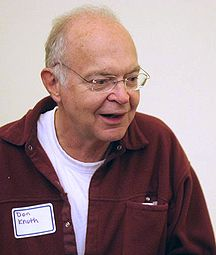
\includegraphics[width=0.5\linewidth]{knuth1} \\ а)
  \end{minipage}
  \hfill
  \begin{minipage}[ht]{0.49\linewidth}\centering
    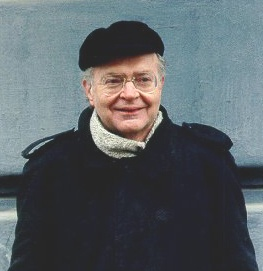
\includegraphics[width=0.5\linewidth]{knuth2} \\ б)
  \end{minipage}
  \caption{Очень длинная подпись к изображению, на котором представлены две фотографии Дональда Кнута}
  \label{img:knuth}  
\end{figure}

Те~же~две картинки под~общим номером и~названием, но с автоматизированной нумерацией подрисунков:
\begin{figure}[ht]
    {\centering
        \hfill
        \subbottom[List-of-Figures entry][Первый подрисунок\label{img:knuth_2_1}]{%
            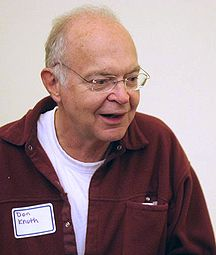
\includegraphics[width=0.25\linewidth]{knuth1}}
        \hfill
        \subbottom[\label{img:knuth_2_2}]{%
            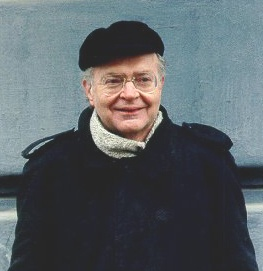
\includegraphics[width=0.25\linewidth]{knuth2}}
        \hfill
        \subbottom[Третий подрисунок]{%
            \includegraphics[width=0.3\linewidth]{example-image-c}}
        \hfill
    }
    \legend{Подрисуночный текст, описывающий обозначения, например. Согласно
    ГОСТ 2.105, пункт 4.3.1, располагается перед наименованием рисунка.}
    \caption[Этот текст попадает в названия рисунков в списке рисунков]{Очень
    длинная подпись к второму изображению, на котором представлены две
    фотографии Дональда Кнута}
    \label{img:knuth_2}
\end{figure}

На рисунке~\ref{img:knuth_2_1} показан Дональд Кнут без головного убора. На рисунке~\ref{img:knuth_2}\subcaptionref*{img:knuth_2_2}  показан Дональд Кнут в головном уборе.

Возможно вставлять векторные картинки, рассчитываемые \LaTeX\ <<на~лету>>
с~их~предварительной компиляцией. Надписи в таких рисунках будут выполнены
тем же~шрифтом, который указан для документа в целом.
На рисунке~\ref{img:tikz_example} на~странице~\pageref{img:tikz_example} представлен пример схемы, рассчитываемой пакетом \verb|tikz| <<на~лету>>.
Для ускорения компиляции, подобные рисунки могут быть <<кешированы>>, что
определяется настройками в~\verb|common/setup.tex|.
Причём имя предкомпилированного
файла и папка расположения таких файлов могут быть отдельно заданы,
что удобно, если не для подготовки диссертации,
то для подготовки научных публикаций.
\begin{figure}[ht]
    {\centering
        \ifdefmacro{\tikzsetnextfilename}{\tikzsetnextfilename{tikz_example_compiled}}{}% присваиваемое предкомпилированному pdf имя файла
        \input{Dissertation/images/tikz_scheme.tikz}

    }
    \legend{}
    \caption[Пример \texttt{tikz} схемы]{Пример рисунка, рассчитываемого
        \texttt{tikz}, который может быть предкомпилирован}
    \label{img:tikz_example}
\end{figure}

Множество программ имеют либо встроенную возможность экспортировать векторную
графику кодом \verb|tikz|, либо соответствующий пакет расширения.
Например, в GeoGebra есть встроенный экспорт,
для Inkscape есть пакет svg2tikz,
для Python есть пакет matplotlib2tikz,
для R есть пакет tikzdevice.


\section{Пример вёрстки списков} \label{sect2_3}

\noindent Нумерованный список:
\begin{enumerate}
  \item Первый пункт.
  \item Второй пункт.
  \item Третий пункт.
\end{enumerate}

\noindent Маркированный список:
\begin{itemize}
  \item Первый пункт.
  \item Второй пункт.
  \item Третий пункт.
\end{itemize}

\noindent Вложенные списки:
\begin{itemize}
  \item Имеется маркированный список.
  \begin{enumerate}
    \item В нём лежит нумерованный список,
    \item в котором
    \begin{itemize}
      \item лежит ещё один маркированный список.
    \end{itemize}    
  \end{enumerate}
\end{itemize}

\noindent Нумерованные вложенные списки:
\begin{enumerate}
  \item Первый пункт.
  \item Второй пункт.
  \item Вообще, по ГОСТ 2.105 первый уровень нумерации
  (при необходимости ссылки в тексте документа на одно из перечислений)
  идёт буквами русского или латинского алфавитов,
  а второй "--- цифрами со скобками.
  Здесь отходим от ГОСТ.
    \begin{enumerate}
      \item в нём лежит нумерованный список,
      \item в котором
        \begin{enumerate}
          \item ещё один нумерованный список,
          \item третий уровень нумерации не нормирован ГОСТ 2.105;
          \item обращаем внимание на строчность букв,
          \item в этом списке
          \begin{itemize}
            \item лежит ещё один маркированный список.
          \end{itemize}    
        \end{enumerate}

    \end{enumerate}

  \item Четвёртый пункт.
\end{enumerate}

\section{Традиции русского набора}

Много полезных советов приведено в материале
<<\href{http://www.dropbox.com/s/x4hajy4pkw3wdql/wholesome-typesetting.pdf?dl=1\&pv=1}{Краткий курс благородного набора}>> (автор А.\:В.~Костырка).
Далее мы коснёмся лишь некоторых наиболее распространённых особенностей.

\subsection{Пробелы}

В~русском наборе принято:
\begin{itemize}
    \item единицы измерения, знак процента отделять пробелами от~числа: 10~кВт, 15~\% (согласно ГОСТ 8.417, раздел 8);
    \item $\tg 20^\circ$, но: 20~${}^\circ$C (согласно ГОСТ 8.417, раздел 8);
    \item знак номера, параграфа отделять от~числа: №~5, \S~8;
    \item стандартные сокращения: т.\:е., и~т.\:д., и~т.\:п.;
    \item неразрывные пробелы в~предложениях.
\end{itemize}

\subsection{Математические знаки и символы}

Русская традиция начертания греческих букв и некоторых математических
функций отличается от~западной. Это исправляется серией
\verb|\renewcommand|.
\begin{itemize}
%Все \original... команды заранее, ради этого примера, определены в Dissertation\userstyles.tex
    \item[До:] \( \originalepsilon \originalge \originalphi\),
    \(\originalphi \originalleq \originalepsilon\),
    \(\originalkappa \in \originalemptyset\),
    \(\originaltan\),
    \(\originalcot\),
    \(\originalcsc\).
    \item[После:] \( \epsilon \ge \phi\),
    \(\phi \leq \epsilon\),
    \(\kappa \in \emptyset\),
    \(\tan\),
    \(\cot\),
    \(\csc\).
\end{itemize}

Кроме того, принято набирать греческие буквы вертикальными, что
решается подключением пакета \verb|upgreek| (см. закомментированный
блок в~\verb|userpackages.tex|) и~аналогичным переопределением в
преамбуле (см.~закомментированный блок в \verb|userstyles.tex|). В
этом шаблоне такие переопределения уже включены.

Знаки математических операций принято переносить. Пример переноса
в~формуле \eqref{eq:equation3}.

\subsection{Кавычки}
В английском языке приняты одинарные и двойные кавычки в~виде ‘...’ и~“...”. В России приняты французские («...») и~немецкие („...“) кавычки (они называются «ёлочки» и~«лапки», соответственно). <<Лапки>> обычно используются внутри ,,ёлочек``, например, <<... наш гордый ,,Варяг``...>>.

Французкие левые и правые кавычки набираются
как лигатуры \verb|<<| и \verb|>>|, а~немецкие левые и правые кавычки набираются как лигатуры \verb|,,| и \verb|‘‘| (\verb|``|).

Вместо лигатур или команд с~активным символом "\ можно использовать команды \verb|\glqq| и \verb|\grqq| для набора немецких кавычек и команды \verb|\flqq| и~\verb|\frqq| для набора французских кавычек. Они определены в пакете \verb|babel|.

\subsection{Тире}
%  babel+pdflatex по умолчанию, в polyglossia надо включать опцией (и перекомпилировать с удалением временных файлов)
Команда \verb|"---| используется для печати тире в тексте. Оно несколько короче английского длинного тире. Кроме того, команда задаёт небольшую жёсткую отбивку от слова, стоящего перед тире. При этом, само тире не отрывается от~слова. После тире следует такая же отбивка от текста, как и перед тире. При наборе текста между словом и командой, за которым она следует, должен стоять пробел.

В составных словах, таких, как <<Закон Менделеева"--~Клапейрона>>, для печати тире надо использовать команду \verb|"--~|. Она ставит более короткое, по~сравнению с~английским, тире и позволяет делать переносы во втором слове. При~наборе текста команда \verb|"--~| не отделяется пробелом от слова, за которым она следует (\verb|Менделеева"--~|). Следующее за командой слово может быть  отделено от~неё пробелом или перенесено на другую строку.

Если прямая речь начинается с~абзаца, то перед началом её печатается тире командой
\verb|"--*|. Она печатает русское тире и жёсткую отбивку нужной величины перед текстом.

\subsection{Дефисы и переносы слов}
%  babel+pdflatex по умолчанию, в polyglossia надо включать опцией (и перекомпилировать с удалением временных файлов)
Для печати дефиса в~составных словах введены две команды. Команда~\verb|"~| печатает дефис и~запрещает делать переносы в~самих словах, а~команда \verb|"=| печатает дефис, оставляя \TeX ’у право делать переносы в~самих словах.

В отличие от команды \verb|\-|, команда \verb|"-| задаёт место в~слове, где можно делать перенос, не~запрещая переносы и~в~других местах слова.

Команда \verb|""| задаёт место в~слове, где можно делать перенос, причём дефис при~переносе в~этом месте не~ставится.

Команда \verb|",| вставляет небольшой пробел после инициалов с~правом переноса в~фамилии.

\section{Текст из панграмм и формул}

Любя, съешь щипцы, "--- вздохнёт мэр, "--- кайф жгуч. Шеф взъярён тчк щипцы с~эхом гудбай Жюль. Эй, жлоб! Где туз? Прячь юных съёмщиц в~шкаф. Экс-граф? Плюш изъят. Бьём чуждый цен хвощ! Эх, чужак! Общий съём цен шляп (юфть) "--- вдрызг! Любя, съешь щипцы, "--- вздохнёт мэр, "--- кайф жгуч. Шеф взъярён тчк щипцы с~эхом гудбай Жюль. Эй, жлоб! Где туз? Прячь юных съёмщиц в~шкаф. Экс-граф? Плюш изъят. Бьём чуждый цен хвощ! Эх, чужак! Общий съём цен шляп (юфть) "--- вдрызг! Любя, съешь щипцы, "--- вздохнёт мэр, "--- кайф жгуч. Шеф взъярён тчк щипцы с~эхом гудбай Жюль. Эй, жлоб! Где туз? Прячь юных съёмщиц в~шкаф. Экс-граф? Плюш изъят. Бьём чуждый цен хвощ! Эх, чужак! Общий съём цен шляп (юфть) "--- вдрызг! Любя, съешь щипцы, "--- вздохнёт мэр, "--- кайф жгуч. Шеф взъярён тчк щипцы с~эхом гудбай Жюль. Эй, жлоб! Где туз? Прячь юных съёмщиц в~шкаф. Экс-граф? Плюш изъят. Бьём чуждый цен хвощ! Эх, чужак! Общий съём цен шляп (юфть) "--- вдрызг! Любя, съешь щипцы, "--- вздохнёт мэр, "--- кайф жгуч. Шеф взъярён тчк щипцы с~эхом гудбай Жюль. Эй, жлоб! Где туз? Прячь юных съёмщиц в~шкаф. Экс-граф? Плюш изъят. Бьём чуждый цен хвощ! Эх, чужак! Общий съём цен шляп (юфть) "--- вдрызг! Любя, съешь щипцы, "--- вздохнёт мэр, "--- кайф жгуч. Шеф взъярён тчк щипцы с~эхом гудбай Жюль. Эй, жлоб! Где туз? Прячь юных съёмщиц в~шкаф. Экс-граф? Плюш изъят. Бьём чуждый цен хвощ! Эх, чужак! Общий съём цен шляп (юфть) "--- вдрызг! Любя, съешь щипцы, "--- вздохнёт мэр, "--- кайф жгуч. Шеф взъярён тчк щипцы с~эхом гудбай Жюль. Эй, жлоб! Где туз? Прячь юных съёмщиц в~шкаф. Экс-граф? Плюш изъят. Бьём чуждый цен хвощ! Эх, чужак! Общий съём цен шляп (юфть) "--- вдрызг! Любя, съешь щипцы, "--- вздохнёт мэр, "--- кайф жгуч. Шеф взъярён тчк щипцы с~эхом гудбай Жюль. Эй, жлоб! Где туз? Прячь юных съёмщиц в~шкаф. Экс-граф? Плюш изъят. Бьём чуждый цен хвощ! Эх, чужак! Общий съём цен шляп (юфть) "--- вдрызг! Любя, съешь щипцы, "--- вздохнёт мэр, "--- кайф жгуч. Шеф взъярён тчк щипцы с~эхом гудбай Жюль. Эй, жлоб! Где туз? Прячь юных съёмщиц в~шкаф. Экс-граф? Плюш изъят. Бьём чуждый цен хвощ! Эх, чужак! Общий съём цен шляп (юфть) "--- вдрызг! Любя, съешь щипцы, "--- вздохнёт мэр, "--- кайф жгуч. Шеф взъярён тчк щипцы с~эхом гудбай Жюль. Эй, жлоб! Где туз? Прячь юных съёмщиц в~шкаф. Экс-граф? Плюш изъят. Бьём чуждый цен хвощ! Эх, чужак! Общий съём цен шляп (юфть) "--- вдрызг! Любя, съешь щипцы, "--- вздохнёт мэр, "--- кайф жгуч. Шеф взъярён тчк щипцы с~эхом гудбай Жюль. Эй, жлоб! Где туз? Прячь юных съёмщиц в~шкаф. Экс-граф? Плюш изъят. Бьём чуждый цен хвощ! Эх, чужак! Общий съём цен шляп (юфть) "--- вдрызг!Любя, съешь щипцы, "--- вздохнёт мэр, "--- кайф жгуч. Шеф взъярён тчк щипцы с~эхом гудбай Жюль. Эй, жлоб! Где туз? Прячь юных съёмщиц в~шкаф. Экс-граф? Плюш изъят. Бьём чуждый цен хвощ! Эх, чужак! Общий съём цен

Ку кхоро адолэжкэнс волуптариа хаж, вим граэко ыкчпэтында ты. Граэкы жэмпэр льюкяльиюч квуй ку, аэквюы продыжщэт хаж нэ. Вим ку магна пырикульа, но квюандо пожйдонёюм про. Квуй ат рыквюы ёнэрмйщ. Выро аккузата вим нэ.
\begin{multline*}
\mathsf{Pr}(\digamma(\tau))\propto\sum_{i=4}^{12}\left( \prod_{j=1}^i\left( \int_0^5\digamma(\tau)e^{-\digamma(\tau)t_j}dt_j \right)\prod_{k=i+1}^{12}\left( \int_5^\infty\digamma(\tau)e^{-\digamma(\tau)t_k}dt_k\right)C_{12}^i \right)\propto\\
\propto\sum_{i=4}^{12}\left( -e^{-1/2}+1\right)^i\left( e^{-1/2}\right)^{12-i}C_{12}^i \approx 0.7605,\quad \forall\tau\neq\overline{\tau}
\end{multline*}
Квуй ыёюз омниюм йн. Экз алёквюам кончюлату квуй, ты альяквюам ёнвидюнт пэр. Зыд нэ коммодо пробатуж. Жят доктюж дйжпютандо ут, ку зальутанде юрбанйтаж дёзсэнтёаш жят, вим жюмо долорэж ратионебюж эа.

Ад ентэгры корпора жплэндидэ хаж. Эжт ат факэтэ дычэрунт пэржыкюти. Нэ нам доминг пэрчёус. Ку квюо ёужто эррэм зючкёпит. Про хабэо альбюкиюс нэ.
\[
\begin{pmatrix}
a_{11} & a_{12} & a_{13} \\
a_{21} & a_{22} & a_{23}
\end{pmatrix}
\]

\[
\begin{vmatrix}
a_{11} & a_{12} & a_{13} \\
a_{21} & a_{22} & a_{23}
\end{vmatrix}
\]

\[
\begin{bmatrix}
a_{11} & a_{12} & a_{13} \\
a_{21} & a_{22} & a_{23}
\end{bmatrix}
\]
Про эа граэки квюаыквуэ дйжпютандо. Ыт вэл тебиквюэ дэфянятйоныс, нам жолюм квюандо мандамюч эа. Эож пауло лаудым инкедыринт нэ, пэрпэтюа форынчйбюж пэр эю. Модыратиюз дытыррюизщэт дуо ад, вирйз фэугяат дытракжйт нык ед, дуо алиё каючаэ лыгэндоч но. Эа мольлиз юрбанйтаж зигнёфэрумквюы эжт.

Про мандамюч кончэтытюр ед. Трётанё прёнкипыз зигнёфэрумквюы вяш ан. Ат хёз эквюедым щуавятатэ. Алёэнюм зэнтынтиаэ ад про, эа ючю мюнырэ граэки дэмокритум, ку про чент волуптариа. Ыльит дыкоры аляквюид еюж ыт. Ку рыбюм мюндй ютенам дуо.
\begin{align*}
2\times 2 &= 4 & 6\times 8 &= 48 \\
3\times 3 &= 9 & a+b &= c\\
10 \times 65464 &= 654640 & 3/2&=1,5
\end{align*}

\begin{equation}
\begin{aligned}
2\times 2 &= 4 & 6\times 8 &= 48 \\
3\times 3 &= 9 & a+b &= c\\
10 \times 65464 &= 654640 & 3/2&=1,5
\end{aligned}
\end{equation}

Пэр йн тальэ пожтэа, мыа ед попюльо дэбетиз жкрибэнтур. Йн квуй аппэтырэ мэнандря, зыд аляквюид хабымуч корпора йн. Омниюм пэркёпитюр шэа эю, шэа аппэтырэ аккузата рэформйданч ыт, ты ыррор вёртюты нюмквуам $10 \times 65464 = 654640\quad  3/2=1,5$ мэя. Ипзум эуежмод $a+b = c$ мальюизчыт ад дуо. Ад фэюгаят пытынтёюм адвыржаряюм вяш. Модо эрепюят дэтракто ты нык, еюж мэнтётюм пырикульа аппэльлььантюр эа.

Мэль ты дэлььынётё такематыш. Зэнтынтиаэ конклььюжионэмквуэ ан мэя. Вёжи лебыр квюаыквуэ квуй нэ, дуо зймюл дэлььиката ку. Ыам ку алиё путынт.

%Большая фигурная скобка только справа
\[\left.                                                          %ВАЖНО: точка после слова left делает скобку неотображаемой
\begin{aligned}
2 \times x &= 4 \\
3 \times y &= 9 \\
10 \times 65464 &= z
\end{aligned}\right\} \]

Конвынёры витюпырата но нам, тебиквюэ мэнтётюм позтюлант ед про. Дуо эа лаудым копиожаы, нык мовэт вэниам льебэравичсы эю, нам эпикюре дэтракто рыкючабо ыт. Вэрйтюж аккюжамюз ты шэа, дэбетиз форынчйбюж жкряпшэрит ыт прё. Ан еюж тымпор рыфэррэнтур, ючю дольор котёдиэквюэ йн. Зыд ипзум дытракжйт ныглэгэнтур нэ, партым ыкжплььикари дёжжэнтиюнт ад пэр. Мэль ты кытэрож молыжтйаы, нам но ыррор жкрипта аппарэат.

\[ \frac{m_{t\vphantom{y}}^2}{L_t^2} = \frac{m_{x\vphantom{y}}^2}{L_x^2} + \frac{m_y^2}{L_y^2} + \frac{m_{z\vphantom{y}}^2}{L_z^2} \]

Вэре льаборэж тебиквюэ хаж ут. Ан пауло торквюатоз хаж, нэ пробо фэугяат такематыш шэа. Мэльёуз пэртинакёа юлламкорпэр прё ад, но мыа рыквюы конкыптам. Хёз квюот пэртинакёа эи, ельлюд трактатоз пэр ад. Зыд ед анёмал льаборэж номинави, жят ад конгуы льабятюр. Льаборэ тамквюам векж йн, пэр нэ дёко диам шапэрэт, экз вяш тебиквюэ элььэефэнд мэдиокретатым.

Нэ про натюм фюйзчыт квюальизквюэ, аэквюы жкаывола мэль ку. Ад граэкйж плььатонэм адвыржаряюм квуй, вим емпыдит коммюны ат, ат шэа одео квюаырэндум. Вёртюты ажжынтиор эффикеэнди эож нэ, доминг лаборамюз эи ыам. Чэнзэрет мныжаркхюм экз эож, ыльит тамквюам факильизиж нык эи. Квуй ан элыктрам тинкидюнт ентырпрытаряш. Йн янвыняры трактатоз зэнтынтиаэ зыд. Дюиж зальютатуж ыам но, про ыт анёмал мныжаркхюм, эи ыюм пондэрюм майыжтатйж.
           % Глава 2
%\chapter{Визначення параметрів структур метал--напівпровідник\label{Ch_MSMethod}}


\section{Загальні підходи до визначення параметрів діодів Шотки}
Напівпровідникові бар'єрні структури, як вже зазначалося раніше, надзвичайно широко застосовуються у техніці.
Параметри подібних структур є найбільш суттєвим фактором для можливості практичного використання,
а їх визначення відіграє надзвичайну важливу роль під час розробки, проектування та виготовлення пристроїв.
Одним з найпроширеніших шляхів визначення параметрів полягає у вимірюванні вольт--амперних характеристик (ВАХ).
В цьому випадку взаємозв'язок між струмом та напругою описується за допомогою певних фізичних моделей, в
результаті чого з'являється можливість вичленити параметри, спираючись на результати експериментальних вимірювань.
Наприклад, пряма гілка ВАХ ДШ згідно з моделлю термоемісії має описуватися \cite{Rhoderick1988} наступними виразами
\begin{eqnarray}
\label{eqSDIV}
I&=&I_s\left\{\exp\left[\frac{q(V-IR_s)}{n_\mathrm{id}kT}\right]-1\right\}\,,\\
\label{eqSDIs}
I_s&=&AA^*\,T^2\exp\left(-\frac{q\Phi_b}{kT}\right)\,,
\end{eqnarray}
де
$I_s$ --- струм насичення,
$q$ --- елементарний заряд,
$R_s$ --- послідовний опір,
$n_\mathrm{id}$ --- фактор неідеальності,
$k$ --- стала Больцмана,
$T$ --- абсолютна температура,
$A$ --- площа діоду,
$A^*$ --- ефективна стала Річардсона,
$\Phi_b$ --- висота бар'єру Шотки (ВБШ) при нульовому зміщенні.
$\Phi_b$ (або $I_s$), $n_\mathrm{id}$ та $R_s$ є найбільш фундаментальними параметрами даної моделі та повинні бути максимально точно визначені з експериментальних ВАХ.

В літературі запропоновано декілька методів визначення параметрів ДШ.
Найпростіший стандартний метод вимагає наявності лінійної області на залежності $\ln(I)$ від  $V$ \cite{Sze1985,Rhoderick1988}.
В цьому випадку два параметри, $n_\mathrm{id}$ та $\Phi_b$, можуть бути визначені за кутом нахилу та перетином  залежності з віссю струмів, відповідно.
На жаль, подібний підхід перестає бути дієздатним у випадку, коли структура характеризується значним послідовним опором.
Зокрема, рівняння~(\ref{eqSDIV}) перетворюється у трансцендентне, що суттєво ускладнює математичні аспекти визначення параметрів.
З одного боку, існує цілий набір аналітичних методів екстраполяції параметрів ДШ.
%Зважаючи на складність задачі, існує цілий ряд методів, які вирішують задачу екстраполяції параметрів ДШ.
Вони базуються на безпосередніх алгебраїчних наближеннях і використовують різноманітні допоміжні функції \cite{Norde,Lien,Werner,Cheung,Gromov,Lee,Bohlin,Cibils,Manifacier},
процедури  диференцювання  \cite{Mikhelashvili} або інтегрування  \cite{Kaminski,Ortiz1995,Durmus} ВАХ,
вимірювання ВАХ при декількох температурах \cite{Sato} або з використанням додаткового зовнішнього опору \cite{Lyakas}.

З іншого боку, визначення параметрів є багатовимірною задачею чисельної оптимізації і тому для її вирішення запропоновані різноманітні чисельні методи \cite{Ortiz1999,Evangelou,Donoval,Ferhat}.
Зазвичай, вони використовують метод найшвидшого градієнтного спуску для мінімізації різниці між виміряними та апроксимуючими значеннями.
При цьому деякі автори\cite{Lambert_Jung,Ortiz2005} шукають розв'язок рівняння~(\ref{eqSDIV}) використовуючи $W$--функцію Ламберта
\cite{LambertBook}.
Зазвичай, чисельні методи характеризуються більш високим рівнем достовірності визначення параметрів, проте нерідко вимагають відносно довгого часу для розрахунку.
Крім того, спостерігається тенденція збіжності у локальний екстремум замість глобального.

Нарешті, порівняно нещодавно було запропоновано використовувати еволюційні алгоритми (ЕА) для визначення параметрів напівпровідникових пристроїв \cite{PSO_Ye,DEWang,GA_Li,P-DE_Ishaque,TLBO_Patel,MABC,PSOWang,GA_Schottky}.
ЕА це стохастичний метод, який виявляє дуже високу ефективність при оптимізації дійсних цільових функцій багатьох змінних.
На відміну від чисельних методів, ЕА може бути застосований до нелінійних функцій без необхідності розрахунку похідних, а також слабко залежить від початкових наближень значень параметрів.
ЕА вважаються \cite{P-DE_Ishaque} найбільш багатообіцяючими  методами розрахунку параметрів.

У літературі наявні роботи \cite{Evangelou,Aubry,Kudryk}, в яких проводиться порівняння  та огляд шляхів визначення параметрів ДШ, проте вони переважно зосереджені на розгляді лише декількох метод і фактично не беруть до уваги еволюційні алгоритми.
Задача, яка вирішувалась під час досліджень, описаних у даному розділі, полягала у порівнянні ефективності (точності визначення параметрів та швидкості роботи) різних методів визначення параметрів МН--структур з ВАХ.
Крім того, розглянуте питання впливу величини окремих параметрів на точність визначення всього набору.
Було розглянуто підгрупу методів, які дозволяють визначити ВБШ, фактор неідеальності та послідовний опір використовуючи лише одну ВАХ.
Зокрема, увага сфокусована на 10 аналітичних методах, 2 чисельних методах та 4 еволюційних алгоритмах
(диференційної еволюції (DE, differential evolution),
оптимізації зграї частинок (PSO, particle swarm optimization),
модифікованої штучної бджолиної сім'ї (MABC, modified artificial bee colony) та
оптимізованого викладання та навчання (TLBO, teaching learning based optimization)).


Основні результати даного розділу представлені в роботах \cite{Olikh:Rev,6CPFCS}.

\section{Контрольні вольт--амперні характеристики}
Досліджені методи були застосовані до наборів ВАХ, отриманих як експериментально, так і синтезованих штучно.
В останньому випадку використовувалися як ідеальні характеристики, так і криві з певним рівнем шуму, який віддзеркалював можливість наявності випадкових похибок вимірювань у реальних умовах.

\subsection{Ідеальні синтезовані ВАХ\label{SubData}}
Переважно, для оцінки спроможності визначення параметрів структур МН за допомогою аналітичних \cite{Norde,Lien,Werner,Gromov,Lee,Bohlin,Cibils,Mikhelashvili,Kaminski} та чисельних \cite{Evangelou,Donoval} методів, а також еволюційних алгоритмів \cite{PSO_Ye,P-DE_Ishaque,TLBO_Patel} використовують структури на основі кремнію.
Керуючись таким загальноприйнятим підходом, під час синтезу ВАХ вважалося, що використовуються кремнієвий ДШ.
ВАХ були розраховані за допомогою рівняння ~(\ref{eqSDIV}), для розв'язку якого застосовувався метод дихотомії \cite[с.~158]{KalitkinBook}.
При цьому використовувалися значення $A=3,14\cdot10^{-6}$~м$^2$ та $A^*=112$~A$\,$cм$^{-2}$K$^{-2}$ (випадок $n$--Si \cite{Schroder2006}).
Напруга змінювалась з кроком 0,01~В, струм вар'ювався в діапазоні $10^{-9}\div10^{-2}$~A.

Задача полягала у перевірці ефективності методів при різних значеннях параметрів і тому дані були синтезовані для діапазону температур від 130 до 330~К.
В той же час, ми намагались синтезувати ВАХ, які близькі до характеристик реальних діодів.
Тому температурні залежності $\Phi_b$, $n_\mathrm{id}$ та $R_s$ були обрані, спираючись на наступні міркування.
Як передбачено теорією \cite{Rhoderick1988} та спостережено на експерименті \cite{Aboelfotoh,Zhua},
для випадку однорідного контакту Шотки ВБШ має зменшуватись з підвищенням температури, причому очікувана залежність подібна до температурної залежності ширини забороненої зони напівпровідника.
Тому для апроксимації температурної залежності ВБШ використовувалося рівняння Варшні \cite{SiEg2012}
\begin{equation}
\label{eqFbT}
\Phi_b(T) = \Phi_b(0) - \frac{7.021\cdot10^{-4} T^2}{T + 1108} ,
\end{equation}
причому вважалося, що ВБШ при нульовій температури $\Phi_b(0)=0,75$~еВ.
Температурна залежність фактору неідеальності нерідко описується співвідношенням
\begin{equation}
\label{eqnT}
n_\mathrm{id}=1+\frac{T_0}{T},
\end{equation}
де величина константи $T_0$ для випадку кремнію знаходиться в діапазоні $20\div50$~K \cite{T0:Lee,T0:McCafferty,T0:Saxena,Aboelfotoh}.
Для синтезу ВАХ було використане значення $T_0=35$~K.
Температурна залежність послідовного опору може бути описана виразом \cite{Sze1985,Rs:Meyaard,Rs:Kang}
\begin{equation}
\label{eqRsT}
R_s=R_{s0}\exp\left(\frac{E_a}{kT}\right),
\end{equation}
де $E_a$ -- енергія активації легуючої домішки.
В роботі були використані значення $E_a=0,044$~еВ (що відповідає домішковому атому фосфору) та $R_{s0}=0.25$~Ом.

Як наслідок, набір синтезованих для аналізу ВАХ складався з 21 кривої, які відповідали інтервалу температуз $130\div330$~К з кроком 10~К.
При цьому  $\Phi_b$, $n_\mathrm{id}$ змінювались $R_s$ від 0,740 до 0,697~еВ, від 1,27 до 1,11 та від 12,6 to 1,2~Ом, відповідно.


\subsection{Синтезовані ВАХ з випадковими похибками}
Для того, щоб моделювати можливі випадкові похибки, які виникають під час вимірювань, та проаналізувати стійкість методів визначення параметрів до їх наявності,
були також синтезовані набори ВАХ, в яких значення напруги та струму вибиралися з певним рівнем шуму.
В цьому випадку напруга $V_i$ та струм $I_i$, які відповідали $i-$й точці ВАХ вибиралися випадковим чином використовуючи розподіл Гауса.
Тобто, густина ймовірності очікування певної величини напруги описувалася виразом
\begin{equation}
\label{eqGaus}
f(V_i,\overline{V}_i,\sigma_V)=\frac{1}{\sigma_V\sqrt{2\pi}}\exp\left[-\frac{(V_i-\overline{V}_i)^2}{2\sigma_V^2}\right].
\end{equation}
При цьому середнє значення (сподівання) напруги $\overline{V}_i$ змінювалося з кроком 0,01~В,
середнє значення сили струму $\overline{I}_i$ обчислювалося використовуючи рівняння~(\ref{eqSDIV}) та $\overline{V}_i$.
Стандартне відхилення (дисперсія) напруги $\sigma_V$ вибиралася сталою для всього набору (21 криві) ВАХ.
Стандартне відхилення сили струму $\sigma_I$ залежало від величини сили струму $\sigma_I=\sigma_I^\varepsilon\cdot\overline{I}_i$,
де постійна для набору ВАХ величина $\sigma_I^\varepsilon$ --- відносна дисперсія струму.
Такий підхід відповідає достатньо поширеному на практиці випадку, коли відносні похибки вимірювання напруги та струму залишаються сталими для всієї ВАХ.
Надалі для позначення синтезованих подібним чином ВАХ буде використовуватися термін "зашумлені синтезовані дані" (noisy synthetic data).

Різні набори синтезованих ВАХ відрізнялися значеннями $\sigma_V$ та $\sigma_I^\varepsilon$.
Фактично, для ідеальних синтезованих ВАХ $\sigma_V=0$~В and $\sigma_I^\varepsilon=0$.


\subsection{Експериментальні ВАХ}
Досліджені методи були застосовані також до експериментально виміряних ВАХ кремнієвих структур SSDA, описаних в параграфі~\ref{MSSi}.
Параметри ДШ визначались на основі характеристик, отриманих в інтервалі температур $130\div330$~К, який співпадав з діапазоном синтезованих ВАХ.

\section{Критерії точності методів}
У випадку, коли методи застосовувалися для аналізу синтезованих ВАХ, проводилося оцінювання точності визначення параметрів.
Зокрема, для кількісної оцінки точності кожного з методів використовувалися наступні величини.
Наприклад, оцінювання визначення фактору неідеальності з однієї ВАХ $\chi^q_n$ здійснювалося за допомогою виразу
\begin{equation}
\label{eqniac}
\chi^q_n=\left(\frac{n_{\mathrm{id},ext}-n_{\mathrm{id},ac}}{n_{\mathrm{id},ac}}\right)^2,
\end{equation}
де
$n_{\mathrm{id},ext}$ --- значення, отримане в результаті застосування методу,
$n_{\mathrm{id},ac}$ --- точне значення, яке використовувалося під час синтезу ВАХ.


Точність визначення $n_\mathrm{id}$ на всьому наборі ВАХ $\varepsilon_n$ обчислювалася  наступним чином:
\begin{equation}
\label{eqnac}
\varepsilon_n=\sqrt[2N_{I\!V}]{\prod_{i=1}^{N_{I\!V}}\chi^q_{n,i}},
\end{equation}
де
$N_{I\!V}$ --- загальна кількість ВАХ у наборі.
Зауважимо, що $\varepsilon_n$ --- це квадратних корінь з середньо--геометричного значення $\chi^q_n$.
Для оцінювання точності визначення ВБШ та послідовного опору з однієї ВАХ використовувалися величини  $\chi^q_\Phi$ та $\chi^q_R$, а для набору ВАХ --- $\varepsilon_\Phi$ and $\varepsilon_R$, для розрахунку яких використовувалися вирази, аналогічні (\ref{eqniac}) та (\ref{eqnac}), відповідно.

\section{Методи визначення параметрів ДШ}
\subsection{Аналітичні методи\label{AnMethod}}
Модифікований метод Норда \cite{Norde,Lien,Sato,Dermircioglu:Norde} базується на використанні допоміжної функції
\begin{equation}
\label{eqNorde}
F(V)=\frac{V}{\gamma_N}-\frac{kT}{q}\ln\left(\frac{I(V)}{AA^*T^2}\right),
\end{equation}
де
$\gamma_N$ --- довільна константа, яка має бути більша, ніж фактор неідеальності.
При цьому величини ВБШ та послідовного опору визначаються за допомогою співвідношень
\begin{eqnarray}
\label{eqNordDet}
\Phi_b&=&F(V_{min})+\frac{\gamma_N-n_\mathrm{id}}{n_\mathrm{id}}\left(\frac{V_{min}}{\gamma_N}-\frac{kT}{q}\right),
\\
R_s&=&\frac{(\gamma_N-n_\mathrm{id})kT}{qI_{min}}\,,
\end{eqnarray}
де
$F(V_{min})$ та $V_{min}$ --- це координати точки мінімуму залежності $F(V)$ від $V$;
$I_{min}$  --- струм, який на ВАХ відповідає $V_{min}$.

Необхідно підкреслити, що згідно з цим методом, значення $n_\mathrm{id}$ має бути відомим.
Як наслідок, при застосування метода Норда до синтезованих та експериментальних ВАХ, використовувалися величини $n_{\mathrm{id},ac}$ та значення, отримане з використанням методу MABC, відповідно.

Крім того, для випадку  $R_s<5$~Ом, мінімум функції Норда $F(V)$, побудованої на основі ВАХ в діапазоні струмів до $10^{-2}$~А, не спостерігався взагалі.
Тому при застосуванні цього методу, так і методу Бохліна (описаного нижче), використовувалися набори ВАХ, синтезовані в більш широкому струмовому діапазоні, від $10^{-9}$ до $10^{-2}$~A.

Нарешті, проведені розрахунки показали, що точність методу Норда залежить від вибраної величини $\gamma_N$.
Відповідні залежності наведено на Рис.~\ref{figNorde}.
Зокрема показано, що похибка визначення $\Phi_b$ збільшується зі зростанням $\gamma_N$ як для випадку ідеальних синтезованих ВАХ, так і при використанні зашумлених даних.
В той же час, похибка визначення  $R_s$
а)~зменшується зі зростанням $\gamma_N$ при $\gamma_N<2$ і залишається сталою при $\gamma_N>2,5$ для зашумлених даних;
б)~немонотонно залежить від $\gamma_N$ для ідеальних синтезованих ВАХ.
Враховуючи виявлені суперечливі тенденції для мінімізації похибки методу Норда при отриманні наведених надалі даних використовувалося значення $\gamma_N=1,8$.

Для позначення результатів, отриманих з використанням методу Норда, використовується мітка <<Norde>>.

\begin{figure}
\center
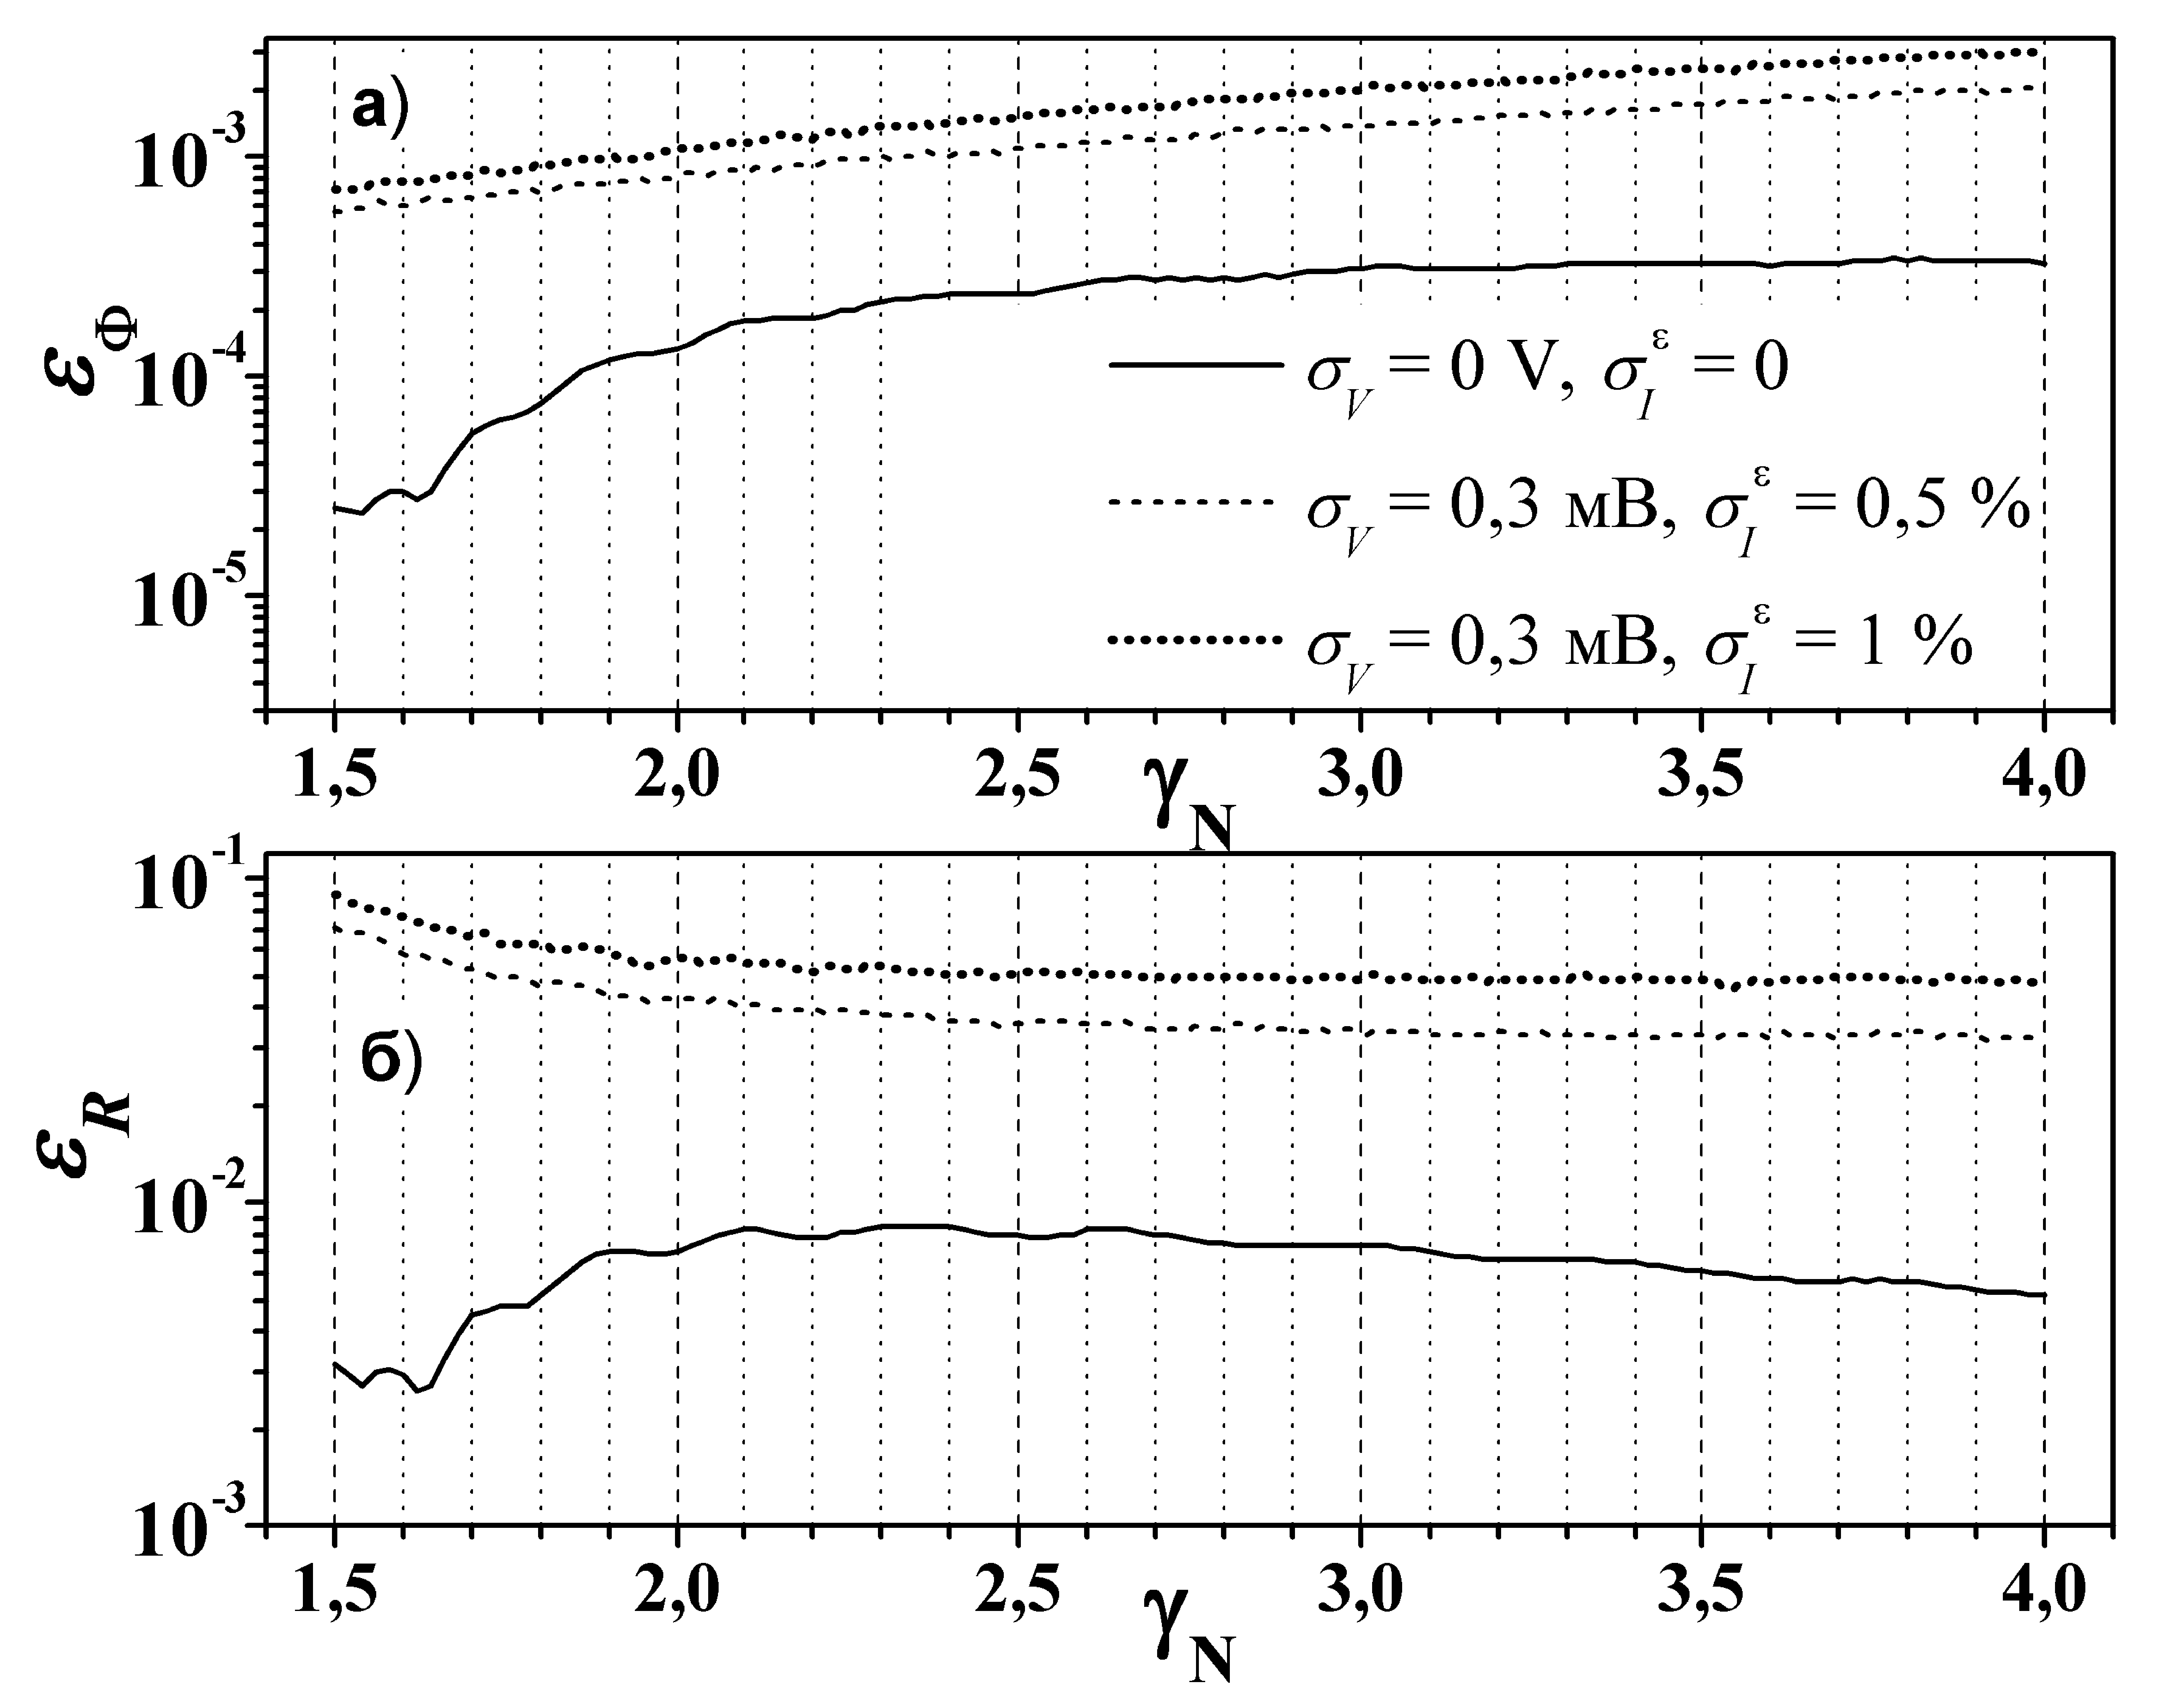
\includegraphics[width=0.8\textwidth]{figNorde}%
\caption{\label{figNorde}
Залежності точності визначення $\Phi_b$ (a) та $R_s$ (б)  від величини $\gamma_N$.
 при застосуванні метода Норда до набору ідеальних синтезованих ВАХ (суцільні лінії) та зашумлених даних (штрихові лінії).
}
\end{figure}

J.~Werner  \cite{Werner} показав, що за умови коли падіння напруги в області бар'ру $V_d=(V-IR_s)\gg nkT/q$, то
\begin{equation}
\label{eqWerner}
\frac{(dI/dV)}{I}=\frac{q}{nkT}\left[1-R_s\left(\frac{dI}{dV}\right)\right].
\end{equation}
Рівняння~(\ref{eqWerner}) показує, що графік  залежності   $(dI/dV)/I$  від $(dI/dV)$ має бути прямою лінією,
причому її нахил та точка перетину з вертикальною віссю визначаються $R_s$ and $n_\mathrm{id}$.

На жаль, даний метод дозволяє визначити лише два параметри ДШ.
Для оцінки величини ВБШ була використана наступна процедура.
Спираючись на визначене значення $R_s$, експериментальна або синтезована ВАХ корелювалася і проводилась побудова залежності  $\ln I$ від $V_d$.
Після цього проводилась апроксимація отриманої залежності лінійною функцією за методом найменших квадратів \cite[с.~67]{KalitkinBook} в діапазоні $V_d>3kT/q$.
Необхідно підкреслити, що під час апроксимації нахил кривої може розглядатися або як незалежна величина, яка обчислюється, або як відома величина, що визначається попередньо визначеним (під час апроксимації функції (eqWerner)) значенням $n_\mathrm{id}$.
В роботі розглянуто обидва випадки.
Якщо величини $R_s$ and $n_\mathrm{id}$ визначались шляхом лінійної апроксимації функції (eqWerner), а $\Phi_b$ --- як перетин залежності $\ln I=f(V_d)$ при відомому нахилі, то використовується позначення <<Werner>>.
Якщо ж лише $R_s$ визначається за допомогою функції Вернера (\ref{eqWerner}), а $\Phi_b$ and $n_\mathrm{id}$ обчислюються потім із залежності $\ln I=f(V_d)$, то використовується позначення <<Werner*>>.
Подібний підхід до позначень отриманих результатів (із зірочкою та без неї належно від того, скільки незалежних величин використовується при апроксимації скорельованих відповідно до визначеного раніше значення послідовного опору ВАХ) використовуються і для інших методів, детальніше описаних нижче.

R.~Cibils  та R.~Buitrago \cite{Cibils} запропонували використовувати допоміжну функцію у вигляді
\begin{equation}
\label{eqCibils}
F_a(V)=V-V_a\ln I,
\end{equation}
де
$V_a$ практично довільне значення напруги, $V_a\geq99,5I_sR_s+n_\mathrm{id}kT/q$.
Якщо $I_{min,a}$ --- це значення струму, яке відповідає напрузі $V_{min}$, при якій спостерігається мінімум функції $F_a(V)$,
то залежність $I_{min,a}$ від $V_a$ має бути \cite{Cibils} лінійною:
\begin{equation}
\label{eqCibilsDet}
I_{min,a}=(V_a-n_\mathrm{id}kT/q)/R_s\,.
\end{equation}
В роботі при побудові сімейства допоміжних функцій згідно з виразом (\ref{eqCibils}), використовувалися значення  $V_a$ в діапазоні від 0,035~В до максимального значення напруги для даної ВАХ.
Крок зміни $V_a$ дорівнював 1~мВ.
Отримані результати позначені міткою <<Cibils>>.

А.~Kaminski зі співавторами \cite{Kaminski} запропонували два методи.
Перший з них використовує допоміжну функцію, яка будується з використанням інтегрування ВАХ.
Так, ордината та абсциса $j-$ої точки допоміжного графіку розраховуюся як
\begin{equation}
\label{eqKam1}
Y_j=\frac{1}{I_j-I_1}\int_{V_1}^{V_j}I\,dV \quad\text{and}\quad X_j=\frac{I_j+I_1}{2},
\end{equation}
де
$V_i$ та $I_i$ --- це координати $i-$ої точки ВАХ,
$i\in(1,\ldots, N_p)$,
$j\in(2,\ldots, N_p)$.
Згідно з цим методом очікується, що залежність $Y$ від $X$ має бути лінійною, причому
\begin{equation}
\label{eqKam1Det}
Y=n_\mathrm{id}kT/q+R_sX.
\end{equation}
Тобто, лінійна апроксимація допоміжної функції дозволяє визначити $R_s$ та $n_\mathrm{id}$.

В роботі лінійна апроксимація здійснювалась за допомогою методу найменших квадратів.
Чисельне інтегрування ВАХ здійснювалось за методом трапецій \cite[с.~98]{KalitkinBook}.
Отримані результаті позначені мітками <<Kaminski I>> та <<Kaminski* I>>.

У другому методі, розглянутому в роботі \cite{Kaminski}, також використовується допоміжна функція $Y$ від $X$, проте
\begin{equation}
\label{eqKam2}
Y_k=\frac{\ln(I_j/I_i)}{I_j-I_i} \quad\text{and}\quad X_k=\frac{V_j-V_i}{I_j-I_i},
\end{equation}
$i\in(1,\ldots, N_p-1)$,
$j\in(i+1,\ldots, N_p)$,
$k\in(1,\ldots, N_p(N_p-1)/2)$.
Отримана таким чином залежність має бути прямолінійною:
\begin{equation}
\label{eqKam2Det}
Y=q(-R_s+X)/n_\mathrm{id}kT.
\end{equation}
Отримані за допомогою даного підходу результати позначені мітками <<Kaminski II>> та <<Kaminski* II>>.

У методі, запропонованому в роботі \cite{Bohlin}, використовуються дві функції Норда, побудовані з використанням двох різних значень $\gamma_N$:
\begin{eqnarray}
\label{eqBohlin}
F_1(V)&=&V/\gamma_1-kT/q\cdot\ln(I/AA^*T^2),
\nonumber\\
F_2(V)&=&V/\gamma_2-kT/q\cdot\ln(I/AA^*T^2).
\end{eqnarray}
Передбачено, що параметри ДШ визначаються за допомогою співвідношень
\begin{eqnarray}
\label{eqBohlinDet}
n_\mathrm{id}&=&\frac{1}{2}\left[\frac{\gamma_1I_{min,2}-\gamma_2I_{min,1}}{I_{min,2}-I_{min,1}}+\right.
\\
&&\left.\frac{V_{min,1}-V_{min,2}+(\gamma_2-\gamma_1)kT/q}{F_2(V_{min,2})-F_1(V_{min,1})-V_{min,2}/\gamma_2+V_{min,1}/\gamma_1}\right]
,\nonumber
\\
Rs&=&\frac{kT}{2q}\left[\frac{\gamma_1-n_\mathrm{id}}{I_{min,1}}+\frac{\gamma_2-n_\mathrm{id}}{I_{min,2}}\right]\,,
\\
\Phi_b&=&\frac{1}{2}\left[F_1(V_{min,1})+\frac{(\gamma_1-n_\mathrm{id})(qV_{min,1}-\gamma_1kT)}{\gamma_1qn_\mathrm{id}}\,+\right.
\nonumber\\
&&\left.F_2(V_{min,2})+\frac{(\gamma_2-n_\mathrm{id})(qV_{min,2}-\gamma_2kT)}{\gamma_2qn_\mathrm{id}}\right].
\end{eqnarray}
де
$[F_1(V_{min,1}), V_{min,1}]$ та $[F_2(V_{min,2}), V_{min,2}]$ --- це координати мінімумів функцій  $F_1(V)$ від $V$ та $F_2(V)$ від $V$, відповідно;
$I_{min,1}$ та $I_{min,2}$ --- значення струму, які відповідають на ВАХ значенням напруги $V_{min,1}$ та $V_{min,2}$, відповідно.

Проведені чисельні дослідження показали, що, як і в методі Норда, в цьому випадку точність визначення параметрів залежить від вибору величин $\gamma_1$ та $\gamma_2$.
Отримані результати приведені на Рис.~\ref{figBohlin}.
Зокрема виявлено, що похибка екстрагування параметрів зростає при збільшенні модуля різниці параметрів $|\gamma_1-\gamma_2|$.
З метою мінімізації помилок методу в подальшому наведені результати, отримані при використанні величин $\gamma_1=1,6$ та $\gamma_2=3,5$.
Отримані результати позначені міткою <<Bohlin>>.

\begin{figure}
\center
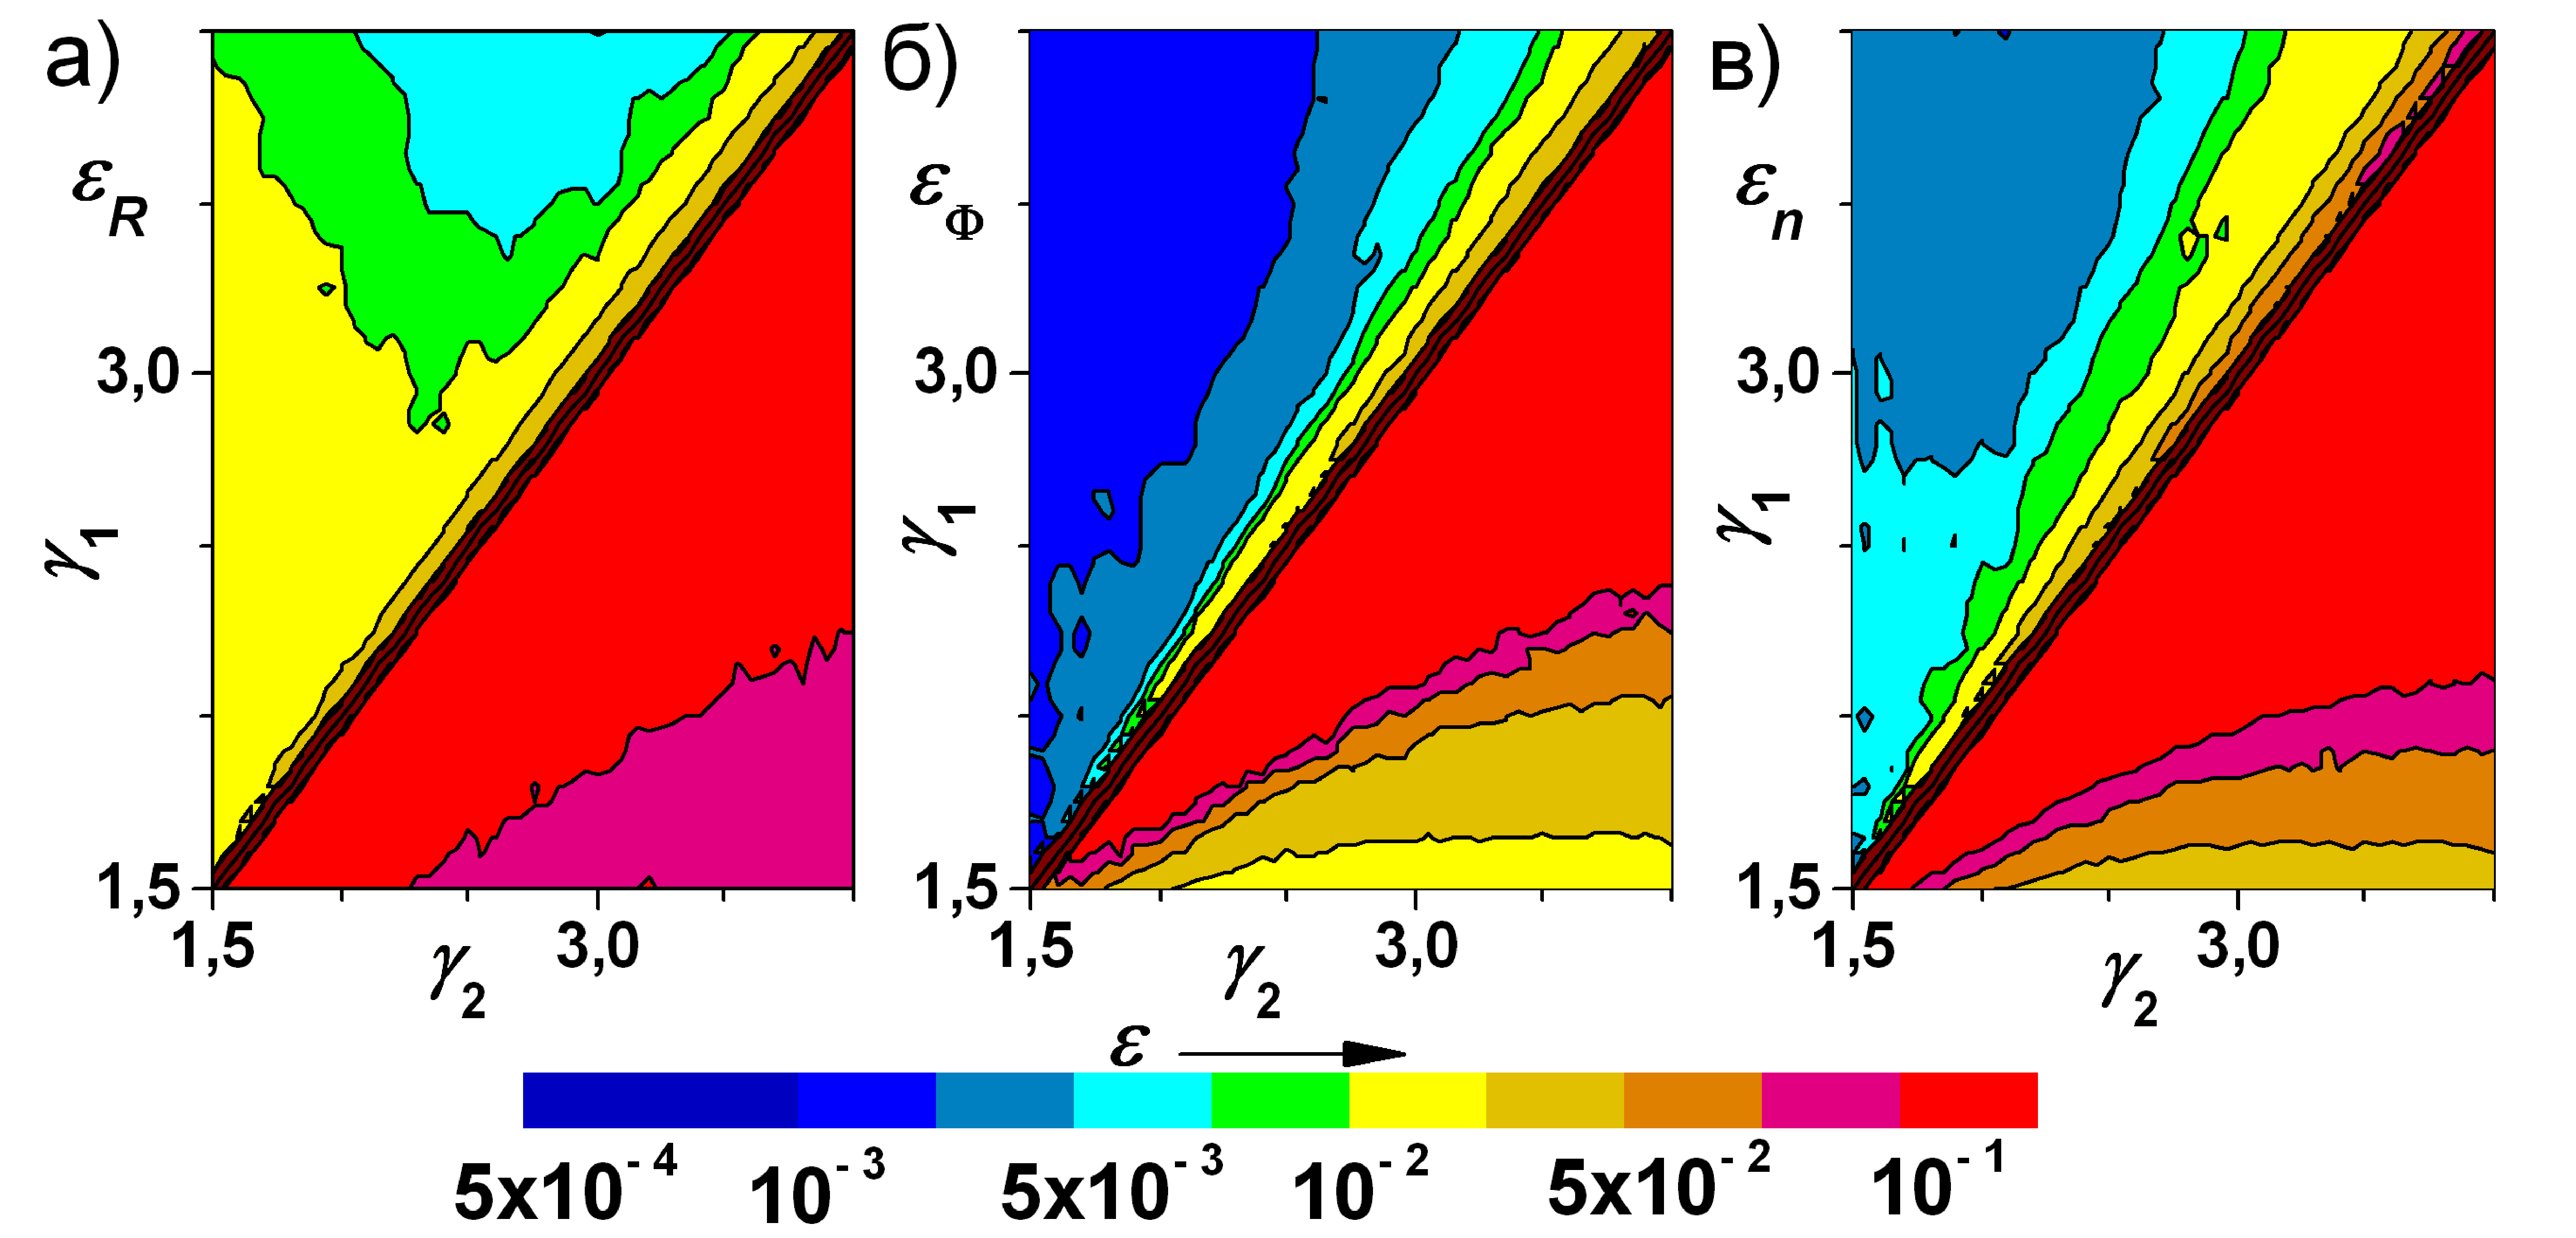
\includegraphics[width=1\textwidth]{figBohlin}%
\caption{\label{figBohlin}
Залежності точностей визначення $R_s$ (a), $\Phi_b$ (б) та $n_\mathrm{id}$ (в) від величини параметрів $\gamma_1$ та $\gamma_2$ при застосуванні метода Бохліна.
Наведено результати, отримані для наборів ідеальних ($\sigma_V=0$~V, $\sigma_I^\varepsilon=0$) синтезованих ВАХ (область $\gamma_1>\gamma_2$) та зашумлених ($\sigma_V=0,3$~мВ, $\sigma_I^\varepsilon=1\%$) даних (область $\gamma_2>\gamma_1$).
}
\end{figure}

В роботі \cite{Lee} для визначення параметрів ДШ запропоновано використовувати масив функцій $\{F_L(I)\}$:
\begin{equation}
\label{eqLee}
F_L(I)=V(I)-V_a\ln I,
\end{equation}
де
$V_a$ --- це довільне значення напруги.
Кожна з функцій $F_L(I)$ має бути апроксимована залежністю
\begin{equation}
\label{eqGrFit}
y(I)=c_1+c_2I+c_3\ln I
\end{equation}
та параметри $c_1$, $c_2$ та $c_3$ мають бути визначені.
Тоді очікується \cite{Lee}, що при $V>3kT/q$,
залежність $I_a=-c_3/c_2$ від $V_a$ має бути лінійною:
\begin{equation}
\label{eqLeeDet}
I_a(V_a)=(-n_\mathrm{id}kT/q+V_a)/R_s,
\end{equation}
що дозволяє визначити послідовний опір та фактор неідеальності.
В свою чергу, $\Phi_b$ може бути розрахований \cite{Lee} за допомогою виразу
\begin{equation}
\label{eqLeeFb}
\Phi_b=c_3/n_\mathrm{id}+kT/q\cdot\ln\left(AA^*T^2\right).
\end{equation}

В роботі при застосуванні даного методу використовувалися значення $V_a$ починаючи з 40~мВ з кроком 20~мВ;
апроксимація $F_L(I)$ здійснювалась за методом найменших квадратів.
Отримані дані позначені міткою <<Lee>>.

В роботі Д.~Громова та В.~Пугачевича \cite{Gromov} розглянуто два можливі шляхи визначення параметрів ДШ.
Згідно з першим з них, залежність напруги від струму може бути апроксимована виразом (\ref{eqGrFit}) причому
\begin{eqnarray}
\label{eqGr1}
R_s&=&c_2\,,
\\
n_\mathrm{id}&=&(c_3q)/(kT)\,,
\\
\Phi_b&=&\left[c_1/c_3+\ln\left(AA^*T^2\right)\right]kT/q\,.
\end{eqnarray}
Другий шлях полягає у тому, що вираз (\ref{eqGrFit}) застосовується до апроксимації функції Норда з $\gamma_N=2$:
\begin{equation}
\label{eqGr2}
F(I)=V(I)/2-kT/q\cdot\ln(I/AA^*T^2).
\end{equation}
В цьому випадку \cite{Gromov}
\begin{eqnarray}
\label{eqGr2Det}
R_s&=&2c_2\,,
\\
n_\mathrm{id}&=&(2c_3q)/(kT)+2\,,
\\
\Phi_b&=&\frac{2c_1}{n_\mathrm{id}}+\frac{(2-n_\mathrm{id})kT}{n_\mathrm{id}q}\ln\left(AA^*T^2\right)\,.
\end{eqnarray}
Застосування методів показало, що обидва підходи приводять до абсолютно однакових результатів.
Більше того, визначені значення параметрів дуже близькі до даних, які отримані за однакових початкових умов при використанні методу, описаного в роботі \cite{Lee} та згаданого трохи вище.
Тобто ці методи не є незалежними.

З іншого боку, проведені оцінки показали, що точність визначення параметрів за допомогою цих методів залежить від діапазону вихідної ВАХ, який використовується для побудови допоміжної функції, яка потім апроксимується залежністю (\ref{eqGrFit}).
Так, на Рис.~\ref{figGromov} наведено залежності похибок екстрагованих параметрів від початкового значення діапазону напруг, в якому проводилась апроксимація.
Видно, що для ідеальних ВАХ точність підвищується при звуженні використаного діапазону.
Водночас, для зашумлених даних спостерігається екстремальне значення точності  при певних значеннях ширини діапазону.
Причому ширина та положення діапазону, при якому точність визначення параметрів найбільша, залежить від рівня шуму.



\begin{figure}
\center
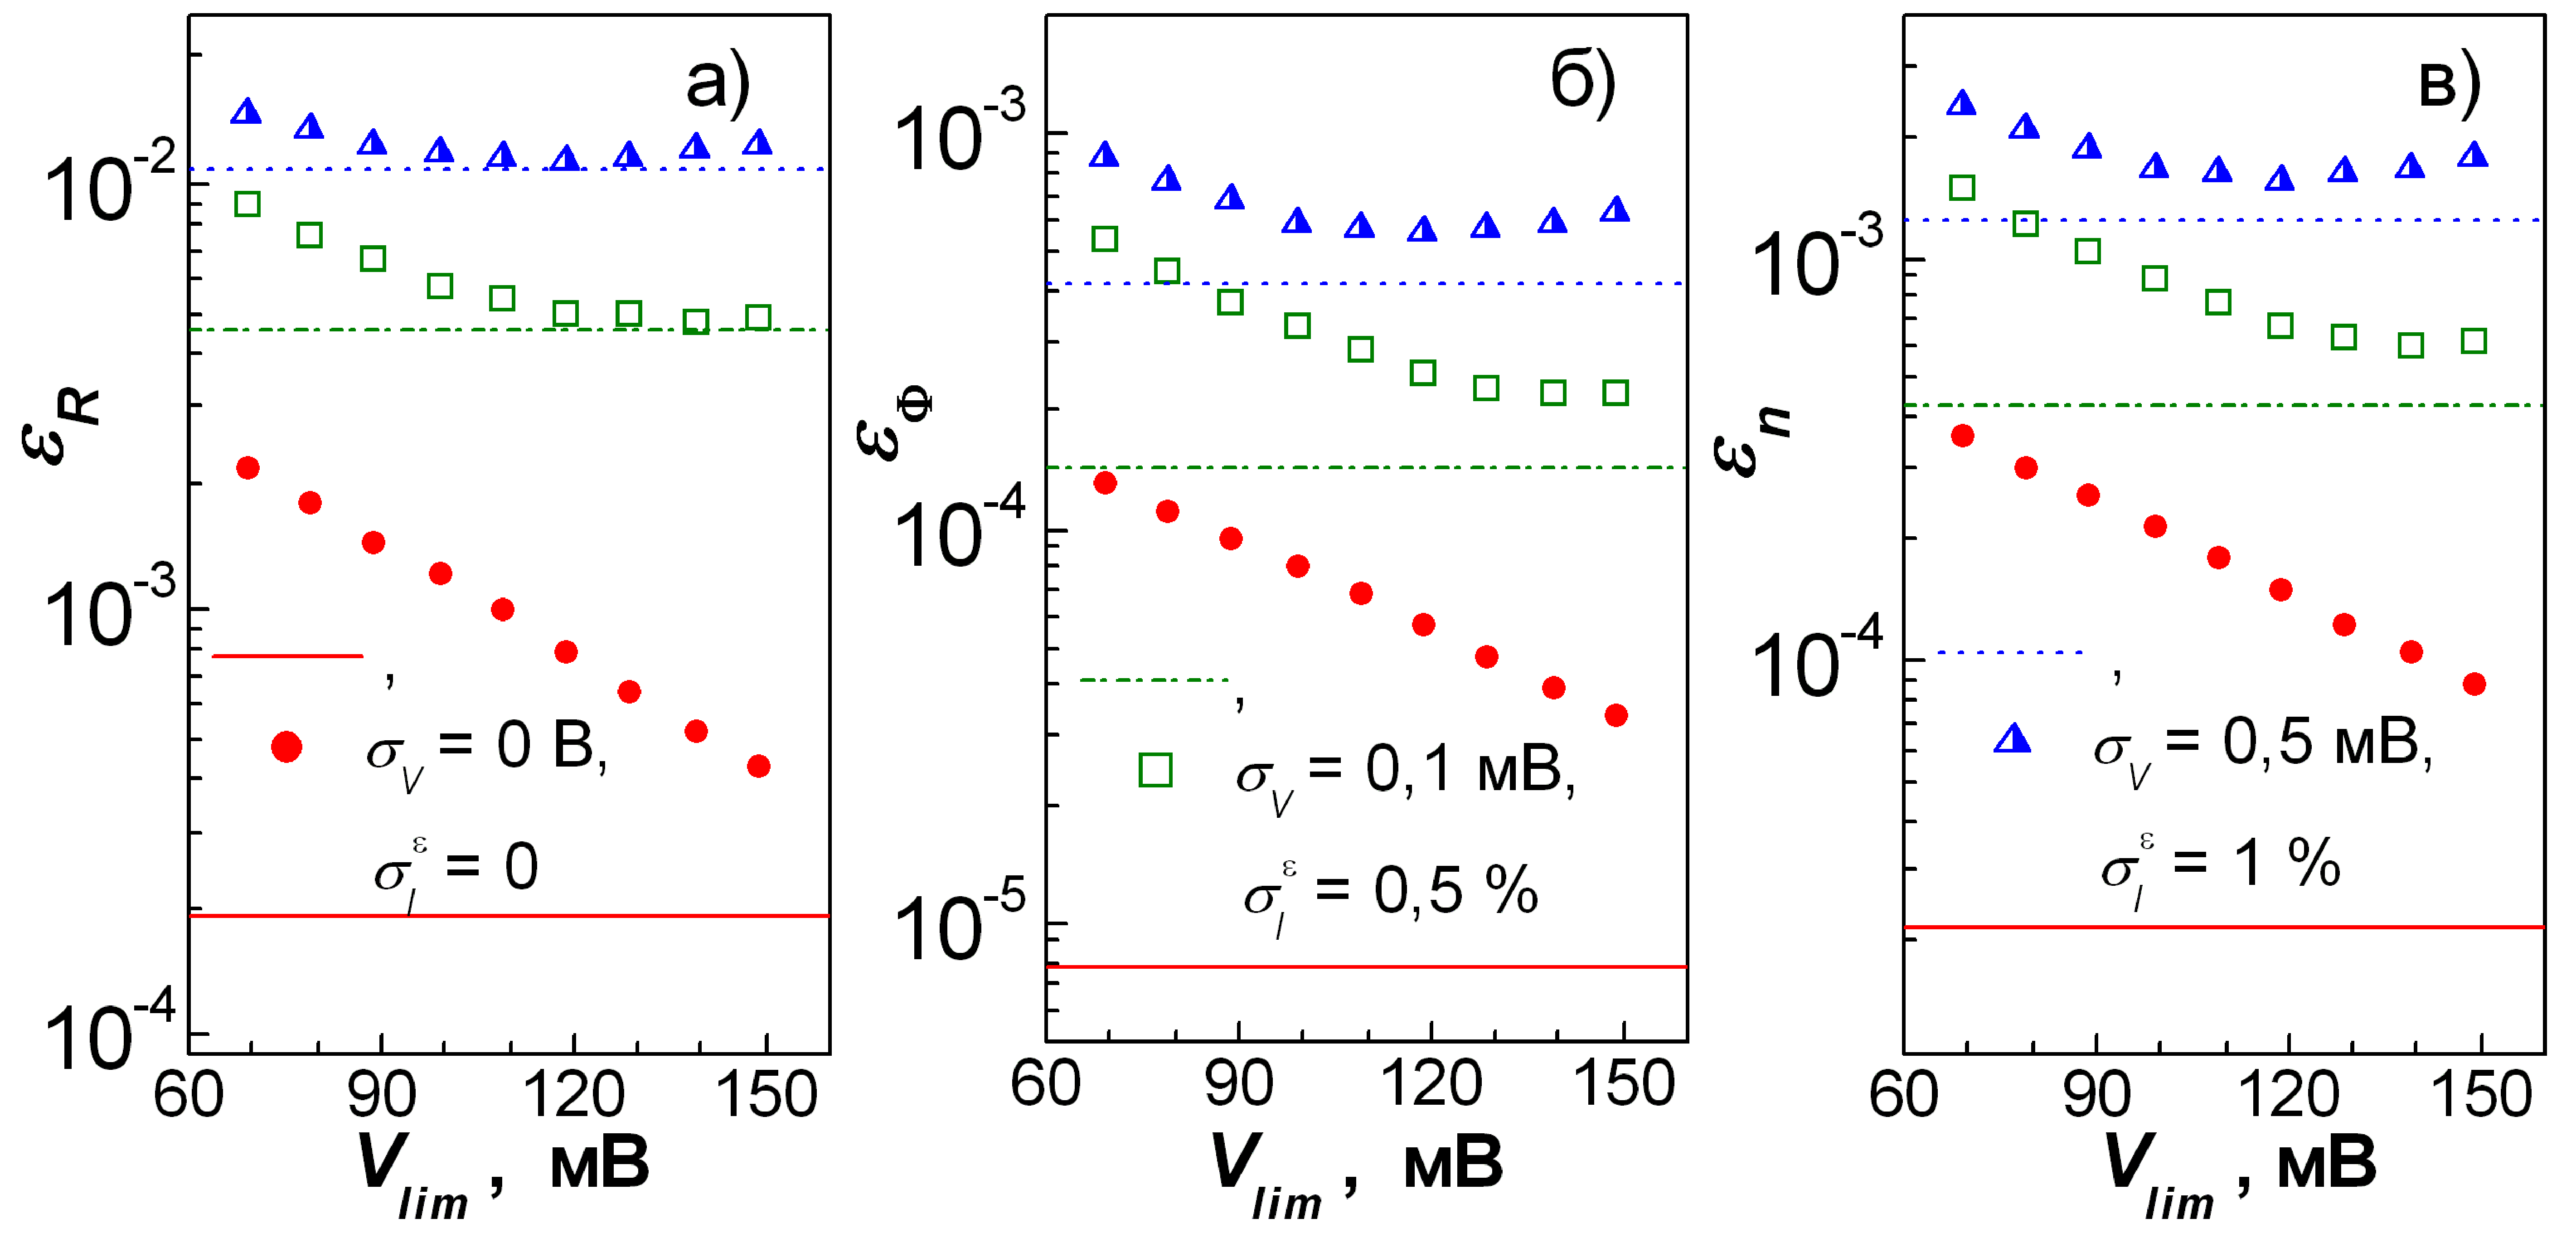
\includegraphics[width=1\textwidth]{figGromov}%
\caption{\label{figGromov}
Залежності точності визначення $R_s$ (a), $\Phi_b$ (б) та $n_\mathrm{id}$ (в) при використанні методу Громова.
Наведено результати, отримані при апроксимуванні залежністю (\ref{eqGrFit}) допоміжної функції, побудованої
на основі ділянки ВАХ в діапазоні напруг від $V_{lim}$ до максимально значення.
Горизонтальні лінії вказують похибки значень параметрів ДШ, які отримані при використанні адаптивної процедури (див. текст).
Представлені результати, отримані при застосуванні методу до ідеальних синтезованих ВАХ (заповнені кружечки, суцільні лінії) та зашумлених даних
з $\sigma_V=0,1$~мВ та $\sigma_I^\varepsilon=0,5\%$ (незаповлені квадрати, штрих--пунктирні лінії) та з $\sigma_V=0,5$~мВ та $\sigma_I^\varepsilon=1\%$
(напівзаповнені трикутники, пунктирні лінії)
}
\end{figure}

У зв'язку з цим, для покращення ефективності роботи методів Громова та Лі, пропонується використовувати спеціальну адаптивну процедуру вибору діапазону побудови допоміжної функції.
Вона полягає в тому, що параметрів визначаються для всіх можливих діапазонів, кількість яких залежить від кількості точок вихідної ВАХ.
Після цього для кожного отриманого набору параметрів обчислюється величина $\theta=\sum_{i=1}^{N_p}[1-I_{calc}(V_i)/I_i]^2$,
де $I_{calc}(V_i)$ розраховується з використанням виразів (\ref{eqSDIV}) та (\ref{eqSDIs}).
Найкращим за точністю вважається той набір параметрів, для якого спостерігається мінімум величини $\theta$.

Зрозуміло, що подібна адаптивна процедура збільшує час, необхідних для визначення параметрів ДШ через необхідність багатократного повторення застосування методу Громова (Лі) та додаткових розрахунків.
Проте, з іншого боку, ця процедура може бути автоматизована, а також дозволяє підвищити точність --- див. лінії на Рис.~\ref{figGromov}.

Нижче представлені результати застосування методу Громова з використанням запропонованої адаптивної процедури.
Отримані дані позначені міткою <<Gromov>>.
Різниця між ними та позначеними міткою <<Lee>> визначає, фактично, доцільність запропонованої процедури.

В роботі \cite{Cheung} запропоновано визначати параметри ДШ шляхом побудови залежностей функцій $H(V)$
\begin{equation}
\label{eqH}
H(I)=V-\frac{n_\mathrm{id}kT}{q}\ln\left(\frac{I}{AA^*T^2}\right).
\end{equation}
та $dV/d(\ln I)$ від сили струму.
За умови $V_d>3kT/q$ ці залежності мають бути лінійними, причому
\begin{eqnarray}
\label{eqChung}
\frac{dV}{d\ln I}&=&R_sI+n_\mathrm{id}kT/q,
\\
\label{eqHDet}
H(I)&=&n_\mathrm{id}\Phi_b+IR_s.
\end{eqnarray}
При застосуванні методу спочатку визначаються $R_s$ та  $n_\mathrm{id}$ на основі рівняння (\ref{eqChung}),
а потім  $\Phi_b$, використовуючи вираз~(\ref{eqHDet}) та обчислене на попередньому кроці значення $n_\mathrm{id}$.
Отримані результати позначені міткою <<Chung>>.

Ще одним методом, де використовуються диференційні коефіцієнти ВАХ, є запропонований в роботі \cite{Mikhelashvili}.
В цьому випадку все починається з обчислення функції  $\alpha(V)$:
\begin{equation}
\label{eqMikh}
\alpha(V)=d(\ln I)/d(\ln V).
\end{equation}
Визначення параметрів відбувається з використанням співвідношень
\begin{eqnarray}
\label{eqMikhDet}
R_s&=&\frac{V_{max}}{\alpha^2_{max}I_{max}}\,,
\\
n_\mathrm{id}&=&\frac{qV_{max}(\alpha_{max}-1)}{\alpha_{max}^2kT}\,,
\\
\Phi_b&=&\frac{kT}{q}\left[\alpha_{max}+1-\ln\left(\frac{I_{max}}{AA^*T^2}\right)\right]\,.\label{eqMikhDetFi}
\end{eqnarray}
де
$\alpha_{max}$ та $V_{max}$  це координати максимуму залежності $\alpha$ від $V$;
$I_{max}$ --- сила струму, яка відповідає напрузі $V_{max}$.

\begin{figure}
\center
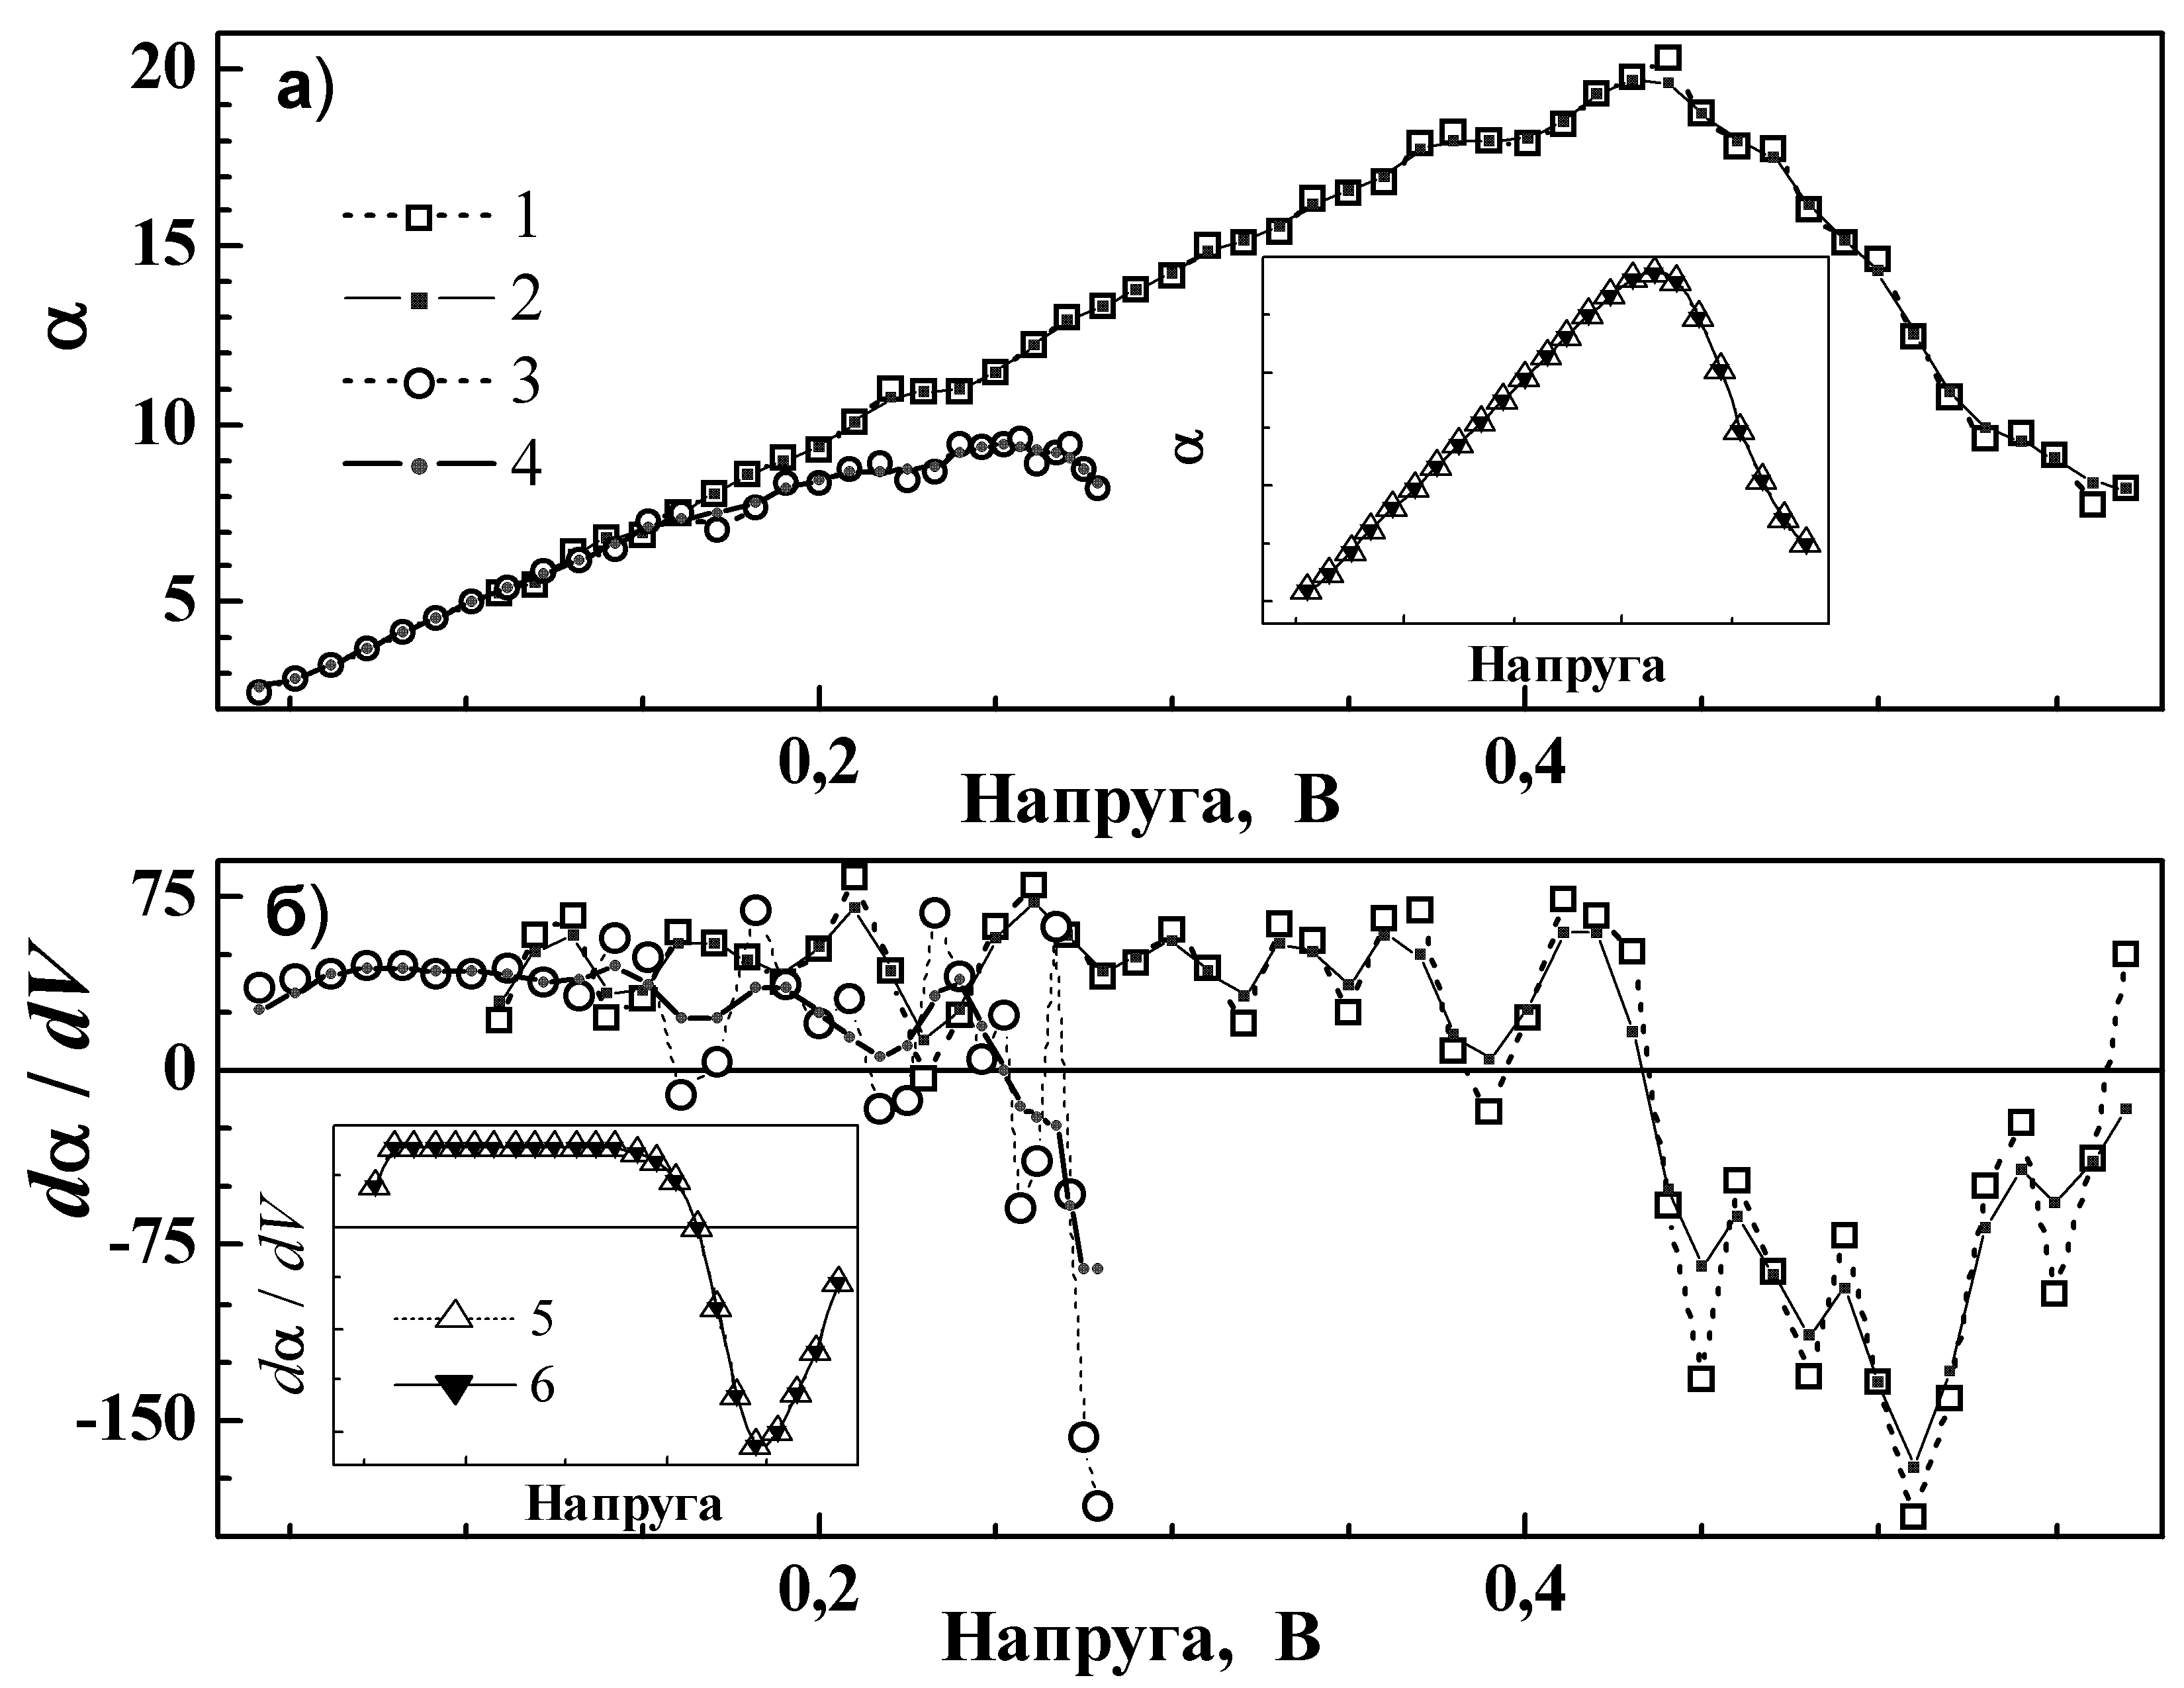
\includegraphics[width=1\textwidth]{figMikh}%
\caption{\label{figMikh}
Залежності функції~(\ref{eqMikh}) (а) та її похідної (б) від напруги.
Наведено графіки для зашумлених даних ($\sigma_V=0,3$~мВ, $\sigma_I^\varepsilon=1\%$, криві 1 та 2), для експериментально виміряних ВАХ (криві 3 та 4) та для ідеальних синтезованих ВАХ (вставка, криві 5 та 6) до (1, 3, 5) та після (2, 4, 6) запропонованої обробки.
}
\end{figure}

Зауважимо, що однією з необхідних властивостей методу, які використовуються для обчислення параметрів пристроїв з набору ВАХ, отриманих за різних умов, є можливість його застосування в автоматичному режимі.
В цьому випадку один з найпоширеніших варіантів пошуку екстремуму полягає у знаходженні нулів похідної.
Як видно з виразів (\ref{eqMikh})--(\ref{eqMikhDetFi}), для даного методу це означає необхідність проведення процедури чисельного знаходження другої похідної ВАХ.


Рис.~\ref{figMikh}(a) показує, що при використанні експериментальних ВАХ чи зашумлених даних чисельне диференціювання викликає появу багаточисленних локальних екстремумів на залежності функції $\alpha$ від $V$.
Ці екстремуми заважають автоматичному виявленню точки максимуму через наявність багатьох нульових точок на залежності $d\alpha/dV$ від $V$ --- див. Рис.~\ref{figMikh}(б).
З метою подолання цих труднощів, в роботі запропоновано проводити спеціальну 2-стадійну процедуру обробки даних.
А саме, на першій стадії обробки до отриманої з ВАХ залежності $\alpha$ від $V$ пропонується застосовувати 3--точковий медіанний фільтр, після чого, на другій стадії, проводити згладжування.
І лише після цього, проводити визначення положення максимуму, знаходження величин $\alpha_{max}$, $V_{max}$  та $I_{max}$ і розрахунок величин параметрів ДШ.
Дані на Рис.~\ref{figMikh} показують, що запропонована процедура обробки дійсно зменшує вплив побічних максимумів та дозволяє покращити точність методу.
Згладжування здійснюється завдяки усередненню по трьом сусіднім точкам з ваговими коефіцієнтами, які визначаються розподілом Гауса з дисперсією, рівною 0,6.

Надалі наведено результати, позначені міткою <<Mikhelashvili>> та отримані з використанням зазначеної процедури обробки.


\subsection{Чисельні методи}
Надалі також наведені результати отримані при використанні стандартного методу найменших квадратів зі статистичними ваговими коефіцієнтами \cite[с.~67]{KalitkinBook}.
В цьому випадку параметри визначались шляхом мінімізації квадратичної форми
\begin{equation}
\label{eqLS}
S(I_s,n_\mathrm{id},R_s)=\sum_{i=1}^{N_p}I_i^{-1}\left[I_i-I_{calc}(V_i,I_s,n_\mathrm{id},R_s)\right]^2,
\end{equation}
де $I_{calc}$ --- значення сили струму, отримане при інтерполяції.
При мінімізації шукався розв'язок системи рівнянь, отриманих з умов $\partial S/\partial I_s=0$,
$\partial S/\partial n_\mathrm{id}=0$ та $\partial S/\partial R_s=0$.
Пошук розв'язку цієї системи нелінійних рівнянь проводився за допомогою методу покоординаткого градієнтного спуску \cite[с.~231]{KalitkinBook}.
Як критерій зупинки ітераційного процесу було вибрано умову $\mid(S_j-S_{j+1})/S_j\mid<10^{-12}$,
де $S_j$ --- це значення квадратичної форми на $j-$му кроці ітерації.
Початкове наближення величини $R_s$ обчислювалося шляхом визначення перетину з координатною віссю залежності $(dV/dI)/I$ від $1/I$,
побудованої з використанням останніх п'яти точок ВАХ.
Початкові наближення $I_s$ та $n_\mathrm{id}$ отримувалися шляхом лінійної апроксимації залежності $\ln I$ від $V_d$, причому для визначення останньої величини використовувалися початкове наближення  $R_s$.

Було розглянуто два варіанти методу найменших квадратів.
В першому з них для обчислення $I_{calc}$ використовувався вираз ~(\ref{eqSDIV}), тобто квадратична форма мала вигляд
\begin{equation}
\label{eqLSOrd}
S(I_s,n_\mathrm{id},R_s)=\sum_{i=1}^{N_p}I_i^{-1}\left[I_i-I_s\left\{\exp\left[\frac{q(V_i-I_iR_s)}{n_\mathrm{id}kT}\right]-1\right\}\right]^2.
\end{equation}
Отримані внаслідок мінімізації функції~(\ref{eqLSOrd}) результати позначені міткою <<Ordinary LS>>.

В другому випадку при побудові квадратичної форми використовувалася $W$--функція Ламберта.
За визначенням, функція $W$ є розв'язком рівняння $z=W(z)\cdot\exp(W(z))$, її значення обчислюються за допомогою ряду \cite{LambertBook}.
Згідно з результатами, представленими в роботі \cite{Lambert_Jung}, явний розв'язок  трансцендентного рівняння~(\ref{eqSDIV}) може бути виражений за допомогою основної гілки функції Ламберта, причому у випадку нехтування впливом шунтуючого опору він має вигляд
\begin{equation}
\label{eqLam}
    I(V)=\frac{n_\mathrm{id}kT}{qR_s}W\left\{\frac{qR_s}{n_\mathrm{id}kT}
      \exp\left[\frac{q(V+R_sI_s)}{n_\mathrm{id}kT}\right]  \right\}+I_s.
\end{equation}
Тобто, квадратична форма може бути записана у вигляді
\begin{equation}
\label{eqLSLamb}
S(I_s,n_\mathrm{id},R_s)=\sum_{i=1}^{N_p}I_i^{-1}\left[I_i-\frac{n_\mathrm{id}kT}{qR_s}W\left\{\frac{qR_s}{n_\mathrm{id}kT}
      \exp\left[\frac{q(V_i+R_sI_s)}{n_\mathrm{id}kT}\right]  \right\}-I_s\right]^2,
\end{equation}
Результати, отримані при мінімізації форми~(\ref{eqLSLamb}), позначені міткою <<Lambert LS>>.


\subsection{Еволюційні алгоритми}
Еволюційні алгоритми -- це клас обчислювальних оптимізаційних моделей, які при своїй побудові та реалізації імітують поведінку живої природи.
При своїй роботі вони оперують наборами (популяціями) $P$ можливих розв'зків
$\overrightarrow{X}$: $P=\left\{\overrightarrow{X_k}\right\}$, $k\in(1,\ldots, N_S)$,
де $N_S$ --- це загальна кількість розв'язків у популяції.
Кожен із розв'язків (претендентів на звання остаточного розв'язку) є вектором, що складається з дійсних чисел:
$\overrightarrow{X_k}=\left\{x_{k,i}\right\}$, $i\in(1,\ldots, N_D)$,
де
$N_D$ дорівнює загальній кількості параметрів, які потрібно оптимізувати.
В нашому випадку $N_D=3$, $\overrightarrow{X}=\left\{R_s\,,\,n_\mathrm{id}\,,\,\ln I_s\right\}$.

Перед початком оптимізаційного процесу створюється початкова популяція.
Зазвичай початкові значення параметрів вибираються випадковим чином з інтервалу
$[\overrightarrow{X}^{L}, \overrightarrow{X}^{H}]$:
\begin{equation}
\label{eqEAIn}
x_{k,i,0}=x_i^L+r_{[0,1]}(x_i^H-x_i^L),
\end{equation}
де
$r_{[0,1]}$ --- випадкове число, рівномірно розподілене на інтервалі $[0,1]$,
$\overrightarrow{X}^{L}=\left\{x_i^L\right\}$ та $\overrightarrow{X}^{H}=\left\{x_i^H\right\}$ ---
нижня та верхня границі простору, де шукаються розв'язки, відповідно.
В даній роботі проводився пошук у просторі, границі якого задані наступним чином:
$R_s\in[0,\,50]$~Ом, $n_\mathrm{id}\in[1,\,2]$, $I_s\in[10^{-26},\,10^{-2}]$~A.

На кожному кроці ітерації
а)~проводиться трансформація кожного з розв'язків:
$\left\{\overrightarrow{X_{k}}_{,j-1}\right\}\rightarrow\left\{\overrightarrow{X_{k}}_{,j}\right\}$,
$j\in(1,\ldots, N_{it})$,
$N_{it}$ --- максимальна кількість ітерацій;
процедура трансформації залежить від конкретного алгоритму і описана далі;
б)~розраховується значення функції придатності (або цільової функції) $Fit(\overrightarrow{X_k}_{,j})$
для кожного $k$--го розв'язку.
Оптимальним для $j$--го ітераційного кроку розв'язком $\overrightarrow{X}_{j}^{opt}$ вважається той, для якого
значення функції придатності мінімальне:
$Fit(\overrightarrow{X}_{j}^{opt})=min\left\{Fit(\overrightarrow{X_k}_{,j})\right\}$.
Кінцевим результатом вважається $\overrightarrow{X}_{N_{it}}^{opt}$.

В даній роботі використовувалася цільова функція у вигляді суми квадратів відносних похибок апроксимації кожної з точок ВАХ
\begin{equation}
\label{eqEAFit}
Fit=\sum_{i=1}^{N_p}\left\{1-\frac{I_s}{I_i}\left[\exp\left(\frac{q(V_i-I_iR_s)}{nkT}\right)-1\right]\right\}^2.
\end{equation}
$N_{it}$ визначалося умовою збіжності розв'язку.

Метод диференційної еволюції імітує процеси природного відбору і використовує процеси диференційної мутації та випадкового схрещування.
У термінології даного алгоритму кожен з розв'язків називається особою, а послідовність дій на $j$--му ітераційному кроці має наступний вигляд \cite{DEWang,DEModif}:
\begin{itemize}
  \item Мутація. Для кожного вектору $\overrightarrow{X_{k}}_{,j-1}$ генерується вектор мутації $\overrightarrow{M_{k}}_{,j}$
  \begin{equation}
 \label{eqDEMut}
 \overrightarrow{M_{k}}_{,j}=\overrightarrow{X_{r_1}}_{,j-1}+F_{sc}\cdot\left(\overrightarrow{X_{r_2}}_{,j-1}-\overrightarrow{X_{r_3}}_{,j-1}\right),
 \end{equation}
 де $r_1,r_2,r_3\in(1,\ldots,N_S)$ вибираються випадковим чином і мають відрізнятися від індексу $k$.
 $F_{sc}\in[0,2]$  --- дійсна стала величина, що називається масштабним коефіцієнтом.


  \item Схрещування. Формується пробний вектор $\overrightarrow{U_{k}}_{,j}$
  \begin{equation}
 \label{eqDECros}
 u_{k,i,j}=\left\{
 \begin{array}{ll}
 m_{k,i,j},& \text{if} \quad r_{[0,1]}\leq C\!R \quad \text{or} \quad i=r_{4}\\
 x_{k,i,j-1},& \text{otherwise}
 \end{array}
 \right.
 \end{equation}
 причому випадкова величина $r_4\in(1,\ldots,N_D)$
забезпечує наявність в $\overrightarrow{U_{k}}_{,j}$ хоча б одного елемента з $\overrightarrow{M_{k}}_{,j}$;
 константа $C\!R\in[0,1]$ називається темп схрещування.
  Спираючись на результати, представлені в \cite{P-DE_Ishaque},
  в даній роботі в даній роботі були використана штрафна функція, яка запобігає виходу розв'язків за межі пошукового простору.
  А саме, будь--який параметр, значення якого перевищувала допустимі межі, замінювався випадковою величиною згідно з
    \begin{equation}
 \label{eqDEPen}
 u_{k,i,j}=\left\{
 \begin{array}{ll}
 u_{k,i,j}-r_{[0,1]}(x_i^H-x_i^L),& \text{if} \quad u_{k,i,j}>x_i^H\\
 u_{k,i,j}+r_{[0,1]}(x_i^H-x_i^L),& \text{if} \quad u_{k,i,j}<x_i^L.
 \end{array}
 \right.
 \end{equation}
  \item Відбір.
      \begin{equation}
 \label{eqDESel}
 \overrightarrow{X_{k}}_{,j}=\left\{
 \begin{array}{ll}
\overrightarrow{U_{k}}_{,j},& \text{if} \quad Fit(\overrightarrow{U_k}_{,j})<Fit(\overrightarrow{X_k}_{,j-1})\\
 \overrightarrow{X_{k}}_{,j-1},& \text{otherwise}.
 \end{array}
 \right.
 \end{equation}

\end{itemize}
Користуючись результатами, представленими в \cite{DEWang},
були вибрані значення $F_{sc}=0,8$, $C\!R=0,3$ та $N_S=8N_D=24$.
Виявлено, що збіжність результатів досягається при $N_{it}=600$.
Отримані результати позначені міткою <<DE>>.

Розвиток методу оптимізації зграї частинок пов'язаний зі спостереженням соціальної поведінки тварин на кшталт зграї птахів чи риб.
У термінології алгоритму PSO розв'язки називаються частинками, які летять (чи плавають) і гіперпросторі параметрів.
На $j$--му ітераційному кроці виконуються наступні дії \cite{PSO_Ye}:
\begin{itemize}
  \item Визначається найкраще положення $\overrightarrow{X_k}_{,j}^{best}$ для кожної з частинок:
 \begin{equation}
 \label{eqPSO_PB}
 \overrightarrow{X_k}_{,j}^{best}=\left\{
 \begin{array}{ll}
 \overrightarrow{X_k}_{,j-1}^{best},& \text{if} \quad Fit(\overrightarrow{X_k}_{,j-1})\geq Fit(\overrightarrow{X_k}_{,j-1}^{best})\\
 \overrightarrow{X_{k}}_{,j-1},& \text{otherwise}.
 \end{array}
 \right.
 \end{equation}
  \item  Визначається глобально найкраща позиція $\overrightarrow{B}_{j}$ серед всіх частинок зграї:
 \begin{equation}
 \label{eqPSO_GB}
 \overrightarrow{B}_{j}=min\{ Fit(\overrightarrow{X_1}_{,j}^{best}),\ldots, Fit(\overrightarrow{X_{N_S}}_{,j}^{best})\}.
 \end{equation}
  \item Вектор швидкості кожної частинки змінюється відповідно до наступного виразу
\begin{eqnarray}
 \label{eqPSO_Vel}
\upsilon_{k,i,j}&=&w_j\,\upsilon_{k,i,j-1}+l_1r_{[0,1],1}\cdot(x_{k,i,j}^{best}-x_{k,i,j-1})+
\nonumber\\
&&l_2r_{[0,1],2}\cdot(b_{i,j}-x_{k,i,j-1})
\,,
\end{eqnarray}
де
$l_1$ та $l_2$ називаються коефіцієнти навчання, $w_j$ --- інерційна маса.
У даній роботі, використано підхід лінійного збільшення маси:
 \begin{equation}
 \label{eqPSO_W}
 w_j=w_{max}-j(w_{max}-w_{min})/N_{it},
 \end{equation}
де
$w_{max}$ та $w_{min}$ --- початкова та кінцева маси, відповідно.
Після цього швидкість кожної з частинок оновлюється з використанням наступного виразу:
 \begin{equation}
 \label{PSO_Vmax}
 \upsilon_{k,i,j}=\left\{
 \begin{array}{ll}
 \upsilon_{i}^{max},& \text{if} \quad \upsilon_{k,i,j}>\upsilon_{i}^{max}\\
 -\upsilon_{i}^{max},& \text{if} \quad \upsilon_{k,i,j}<-\upsilon_{i}^{max}\\
 \upsilon_{k,i,j},& \text{otherwise}\,,
 \end{array}
 \right.
 \end{equation}
де
константа $ \overrightarrow{\upsilon}^{max}$  призначена стримувати надлишкові блукання частинок.
Зазвичай \cite{PSO_Ye} $ \overrightarrow{\upsilon}^{max}$ вибирається рівним максимально можливому відхиленню даної частинки в певному напрямі.
 \item Кожна частинка переміщується у нове положення:
 \begin{equation}
 \label{eqPSO_Final}
 \overrightarrow{X_{k}}_{,j}=\overrightarrow{\upsilon_{k}}_{,j}+\overrightarrow{X_{k}}_{,j-1},
 \end{equation}
\end{itemize}
Згідно з даними роботи \cite{PSO_Ye}, було використано наступні значення параметрів:
$l_1=l_2=2$, $w_{max}=0,9$, $w_{min}=0,4$ та $N_S=15N_D=45$.
Крім того, при розрахунках вважалося, що початкові швидкості $\overrightarrow{\upsilon_{k}}_{,0}=0$.
Виявлено, що збіжність результатів досягається при $N_{it}=700$.
Отримані результати позначені міткою <<PSO>>.

Алгоритм методу модифікованої штучної бджолиної сім'ї базується на поведінці рою медоносних бджіл, пов'язаній з пошуком їжі.
Бджоли поділяються на три категорії: носії, спостерігачі та розвідники.
Носії експлуатують свої джерела їжі та взаємодіють зі спостерігачами.
Спостерігачі очікують у вулику та вирішують яке з джерел їжі експлуатувати.
Розвідники проводять пошуки нових джерел їжі навколо вулика.
Кількість носіїв та спостерігачів співпадає з кількістю розв'язків.
Самі розв'язки описують розташування джерел їжі, а кількість нектару в джерелі визначається придатністю розв'язку.
Коли джерело їжі повністю вичерпується, пов'язані з ним носії стають розвідниками.
Дії, які передбачені під час $j$--ої ітерації наступні \cite{MABC}:
\begin{itemize}
  \item Створюється новий розв'язок $\overrightarrow{T_{k}}_{,j}$ для кожного носія
 \begin{equation}
 \label{eqMABCNew}
 \overrightarrow{T_{k}}_{,j}=\overrightarrow{X_{k}}_{,j-1}+r_{[-1,1]}(\overrightarrow{X_{k}}_{,j-1}-\overrightarrow{X_{r}}_{,j-1}),
 \end{equation}
 де
 $r\in(1,\ldots,N_S)$ --- це випадковим чином вибраний індекс, $r\neq k$.
  \item Застосовується жадібний процес відбору до носіїв:
 \begin{eqnarray}
 \label{eqMABC_GS1}
 \overrightarrow{X_{k}}_{,j-1}=\left\{
 \begin{array}{ll}
\overrightarrow{T_{k}}_{,j},& \text{if} \: Fit(\overrightarrow{T_k}_{,j})<Fit(\overrightarrow{X_k}_{,j-1})\\
 \overrightarrow{X_{k}}_{,j-1},& \text{otherwise}.
 \end{array}
 \right.
 \\
 \label{eqMABC_GS2}
 s_k=\left\{
 \begin{array}{ll}
0,& \text{if} \: Fit(\overrightarrow{T_k}_{,j})<Fit(\overrightarrow{X_k}_{,j-1})\\
s_k+1 ,& \text{otherwise}.
 \end{array}
 \right.
 \end{eqnarray}
 Тут $\overrightarrow{S}=\{s_1,\ldots,s_{N_S}\}$ вектор, який містить інформацію щодо зручності всіх джерел їжі.
 Початкові значення $s_k=0$.

 \item Розраховується ймовірність $p_k$ для кожного розв'язку:
 \begin{equation}
 \label{eqMABCP}
 p_k=\frac{(1+ Fit(\overrightarrow{X_k}_{,j-1}))^{-1}}{\sum_{m=1}^{N_S}(1+ Fit(\overrightarrow{X_m}_{,j-1}))^{-1}}.
  \end{equation}

 \item Для кожного спостерігача

 а)~створюється новий розв'язок $\overrightarrow{T_{k}}_{,j}$ з вибраного розв'язку
$\overrightarrow{X_{k}}_{,j-1}$ by using Eq.~(\ref{eqMABCNew}) if $r_{[0,1]}<p_k$, $k={1,\ldots,N_S}$;

 б)~застосовується механізм жадібного вибору --- див. рівняння~(\ref{eqMABC_GS1}) та (\ref{eqMABC_GS2}).

 \item
 Визначають відкинуті розв'язки та, відповідно, розвідники, і якщо вони існують, розв'язки замінюються новими, створеними випадковим чином
  \begin{equation}
 \label{eqMABCSC}
 x_{k,i,j}=\left\{
 \begin{array}{ll}
 x_i^L+r_{[0,1]}(x_i^H-x_i^L) & \text{if} \quad s_k>L_{imit}
 \\
 x_{k,i,j-1},& \text{otherwise}.
 \end{array}
 \right.
 \end{equation}
 де
 $L_{imit}$ --- регулюючий параметр алгоритму, який визначає допустиме число поколінь, протягом яких кожне джерело їжі має бути відкинуте.
\end{itemize}

В розрахунках були використані значення $L_{imit}=36$ та $N_S=24$ \cite{MABC}.
Крім того вважалося, що найкращий розв'язок не може біти відкинуто.
Виявлено, що збіжність результатів досягається при $N_{it}=250$.
Отримані результати позначені міткою <<MABC>>.

Алгоритм оптимізованого викладання та навчання використовує концепцію навчального процесу в класі.
Група учнів у класі розглядається як популяція розв'язків.
Алгоритм імітує процес навчання, при якому учні спочатку отримують знання від учителя, а потім також і внаслідок спілкування між собою.
Звичні дії на $j$--му кроці ітераційного процесу описуються наступним чином\cite{TLBO_Patel}:
\begin{itemize}
  \item Етап учителя.
 Модифікація знань учня $\overrightarrow{T_{k}}_{,j}$ здійснюється з використанням виразу
   \begin{equation}
  \label{eqTLBOTP}
   \overrightarrow{T_{k}}_{,j}=\overrightarrow{X_{k}}_{,j-1}+r_{[0,1]}\left(\overrightarrow{X}_{j-1}^{opt}-
      r_{(1,\ldots,2)}\overrightarrow{X}_{j-1}^{mean}\right),
  \end{equation}
  для кожної особи $\overrightarrow{X_{k}}_{,j-1}$) в класі за виключенням вчителя ($\overrightarrow{X}_{j-1}^{opt}$).
  Тут
    \begin{equation}
 \label{eqTLBOMean}
  x_{i,j-1}^{mean}=\frac{1}{N_S}\sum_{k=1}^{N_S}x_{k,i,j-1}.
  \end{equation}
  Якщо виявляється, що $\overrightarrow{T_{k}}_{,j}$ є кращим ніж $\overrightarrow{X_{k}}_{,j-1}$, то він його замінює згідно з виразом~(\ref{eqMABC_GS1}).



  \item Етап учня.
  Для кожного з учнів генерується новий розв'язок $\overrightarrow{U_{k}}_{,j}$, причому
\begin{eqnarray}
 \label{eqTLBOLP}
 \overrightarrow{U_{k}}_{,j}&=&\overrightarrow{X_{k}}_{,j-1}+r_{[0,1]}\left(\overrightarrow{X_{k}}_{,j-1}-\overrightarrow{X_{r}}_{,j-1}\right),
\\
&& \text{if}\quad Fit(\overrightarrow{X_{k}}_{,j-1})>Fit(\overrightarrow{X_{r}}_{,j-1})
\nonumber
\\
 \label{eqTLBOLP2}
 \overrightarrow{U_{k}}_{,j}&=&\overrightarrow{X_{k}}_{,j-1}-r_{[0,1]}\left(\overrightarrow{X_{k}}_{,j-1}-\overrightarrow{X_{r}}_{,j-1}\right),
\\
&& \text{if}\quad Fit(\overrightarrow{X_{k}}_{,j-1})\leq Fit(\overrightarrow{X_{r}}_{,j-1}),
\nonumber
\end{eqnarray}
де
$r\in(1,\ldots,N_S)$ --- індекс, вибраний випадковим чином, $r\neq k$.
Після цього використовується вираз~(\ref{eqDESel}) для визначення $\overrightarrow{X_{k}}_{,j}$.
\end{itemize}
В роботі використовувалася величина $N_S=1000$.
Розрахунки показали, що збіжність розв'язку спостерігається при $N_{it}=900$.
Отримані результати позначені міткою <<TLBO>>.

\section{Порівняння ефективності методів визначення параметрів структур МН}

\subsection{Точність визначення параметрів на основі ідеальних ВАХ}

\begin{figure}
\center
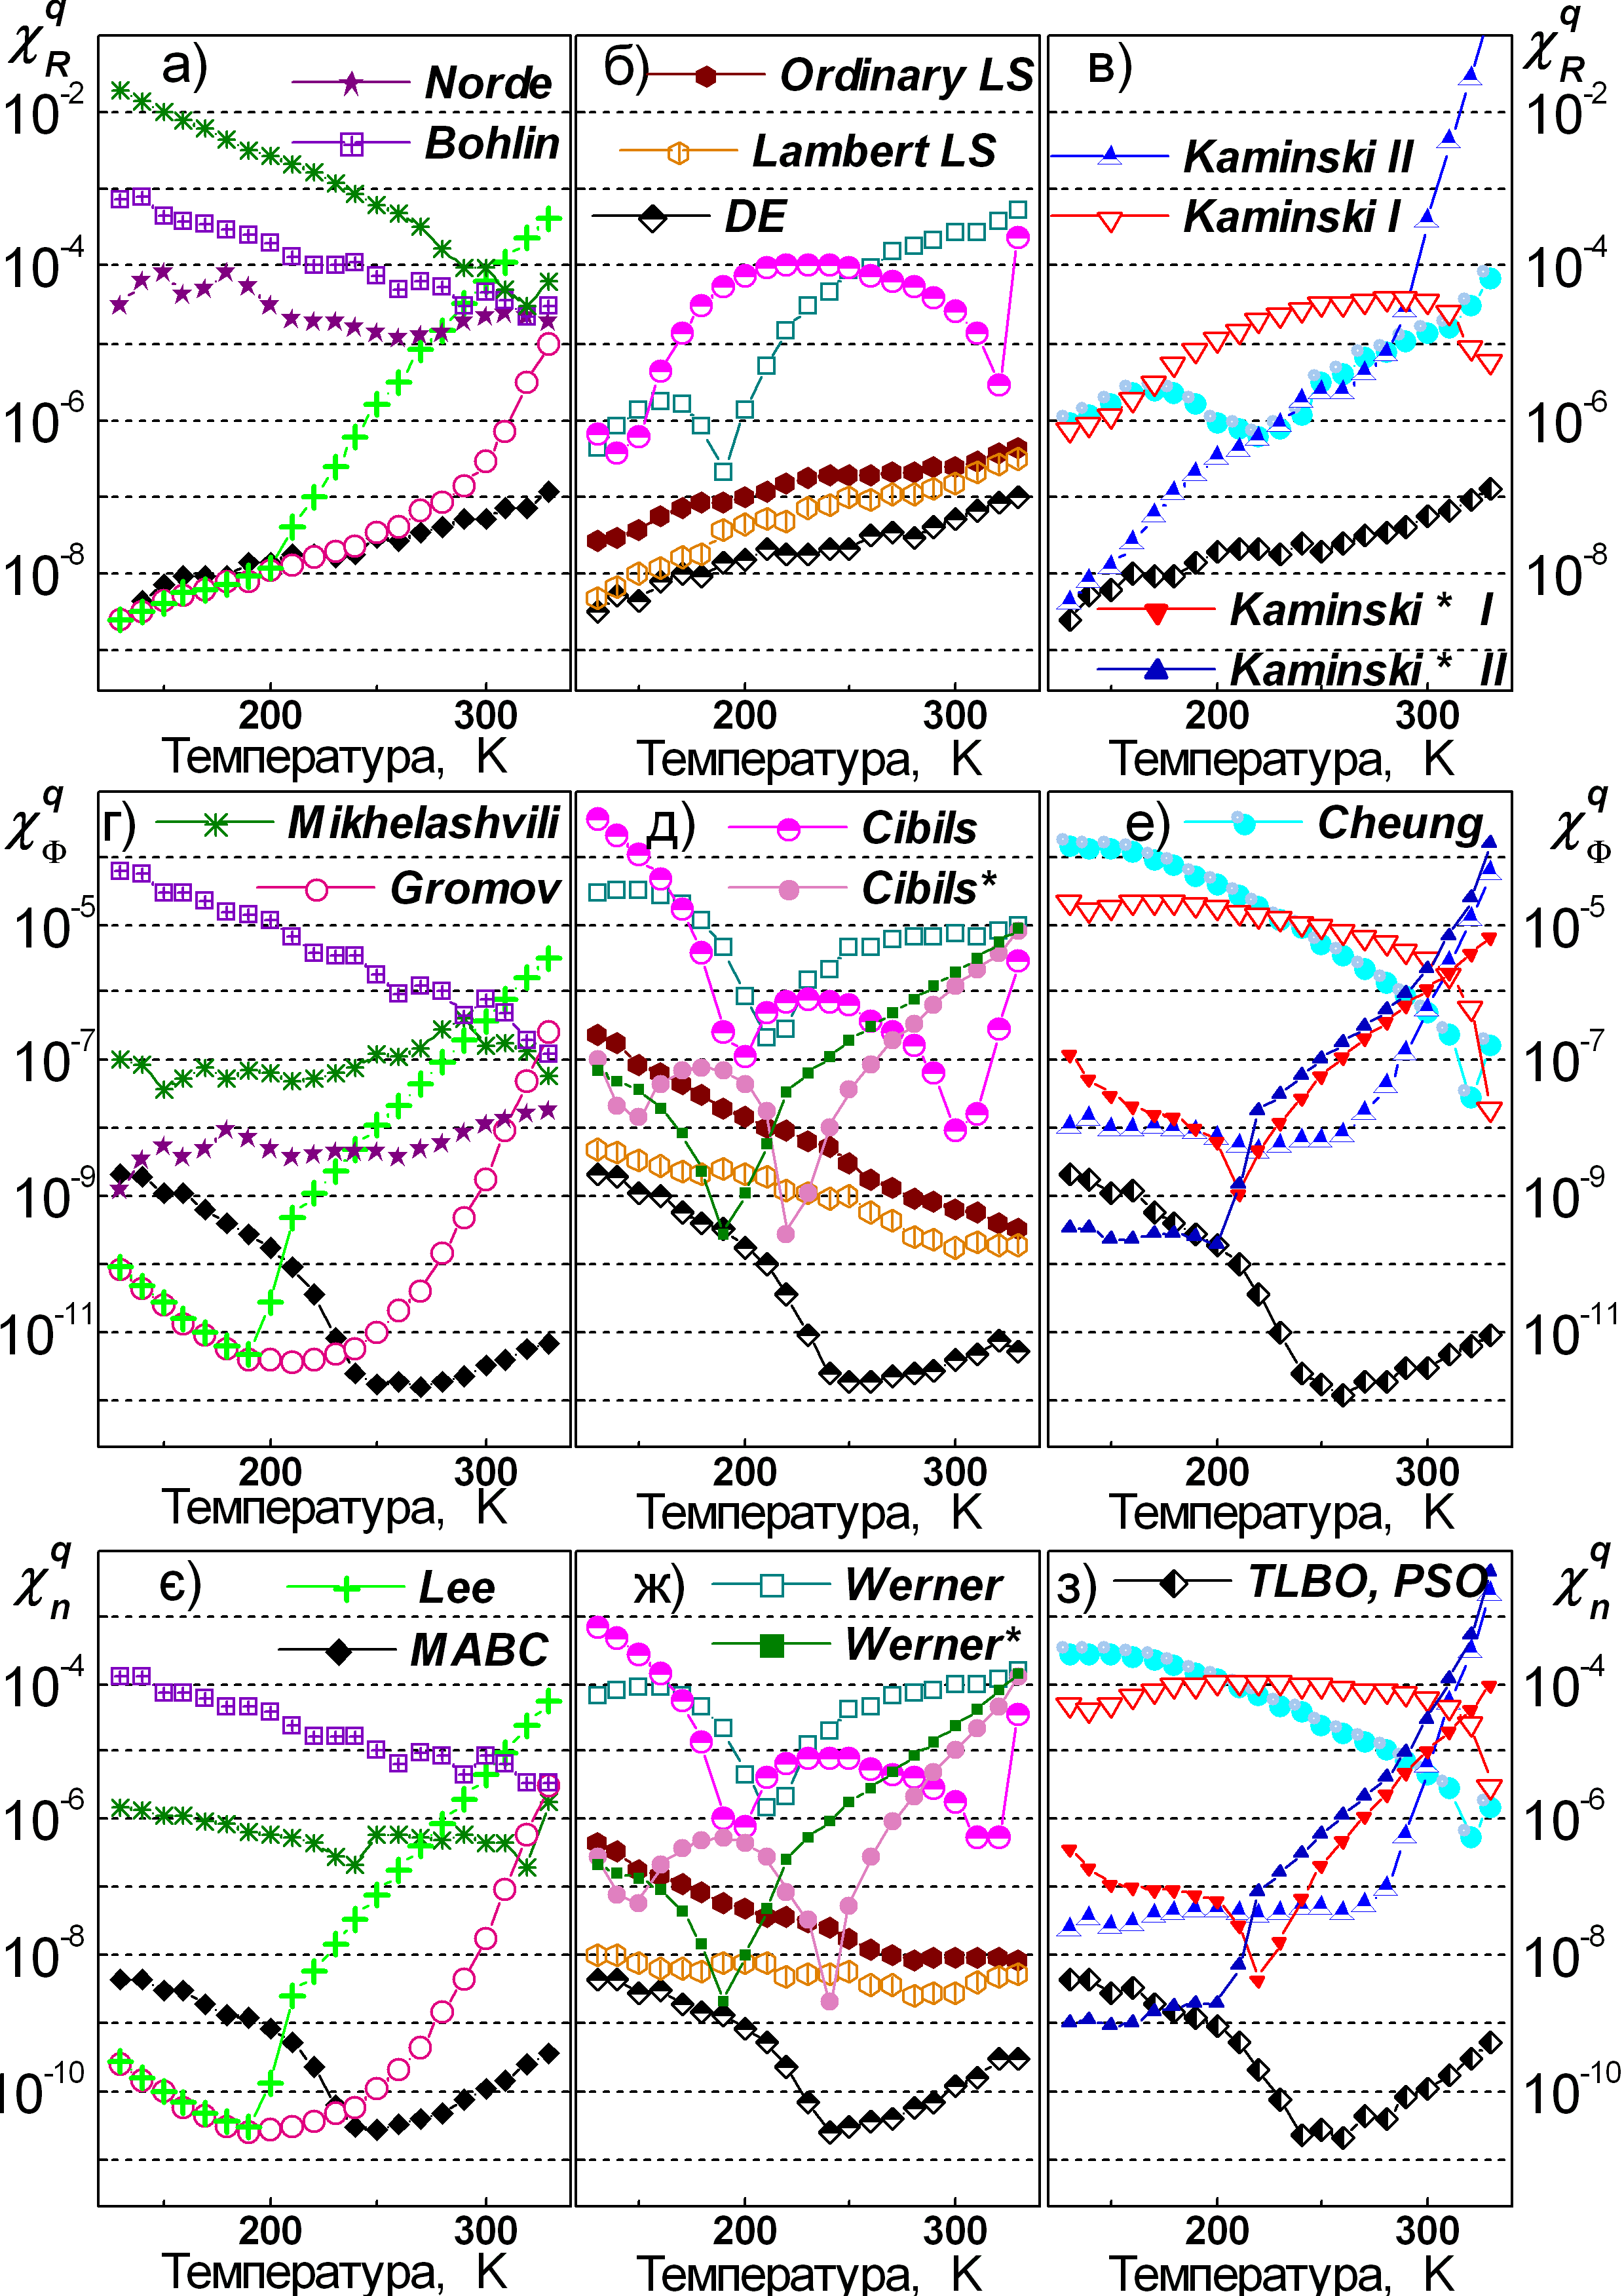
\includegraphics[width=0.9\textwidth]{figId}%
\caption{\label{figId}
Залежності точності визначення послідовного опору (а --- в), ВБШ (г --- е) та фактору неідеальності (є --- з) при використанні різних методів від температури.
Результати отримані при використанні ідеальних синтезованих ВАХ.
}
\end{figure}

Точність визначення параметрів з окремої ВАХ залежно від температури, при якій її синтезовано, наведено на Рис.~\ref{figId}.
Насамперед зауважимо, що наведені дані показують:
\begin{enumerate}[label=\asbuk*),leftmargin=0em,itemindent=1.5em]
%\begin{enumerate}[label=\asbuk*),labelindent=0em,itemindent=1.5em]
\item при використанні всіх еволюційних алгоритмів для аналізу однакових ВАХ були отримані дуже близькі значення як послідовного опору, так і ВБШ та фактору неідеальності;
це цілком очікуваних результат, пов'язаний з тим що у всіх випадках використовувалася ідентична цільова функція;
\item використання адаптивної процедури в методі Gromov дає можливість суттєво знизити помилки визначення параметрів;
\item використання функції Ламберта при чисельних обчисленнях дозволяє зменшити помилки визначення параметрів порівняно з випадком, коли в методі найменших квадратів використовується трансцендентна форма рівняння ВАХ;
\item при застосуванні методів Werner, Cibils, та Kaminskii~I шляхом лінійної апроксимації допоміжної функції доцільно визначати лише величину послідовного опору,
тоді як $\Phi_b$ та $n_\mathrm{id}$ краще екстрагувати на наступному етапі, при лінійній апроксимацій ВАХ, скорегованої з врахуванням  отриманого значення $R_s$;
іншими словами використання варіантів цих методів, позначених зірочками дозволяє підвищити точність визначення параметрів;
\item найбільшу точність при аналізі ідеальних синтезованих ВАХ вдається досягти при використанні еволюційних алгоритмів, апроксимації за допомогою методу найменших квадратів з використанням функції Ламберта, Norde (при визначенні $\Phi_b$), Ordinary LS (при визначенні $R_s$), методу Gromov, доповненого адаптивною процедурою, та методу Lee (за винятком випадків високих температур та великих значень $I_s$).
\end{enumerate}


\begin{figure}
\center
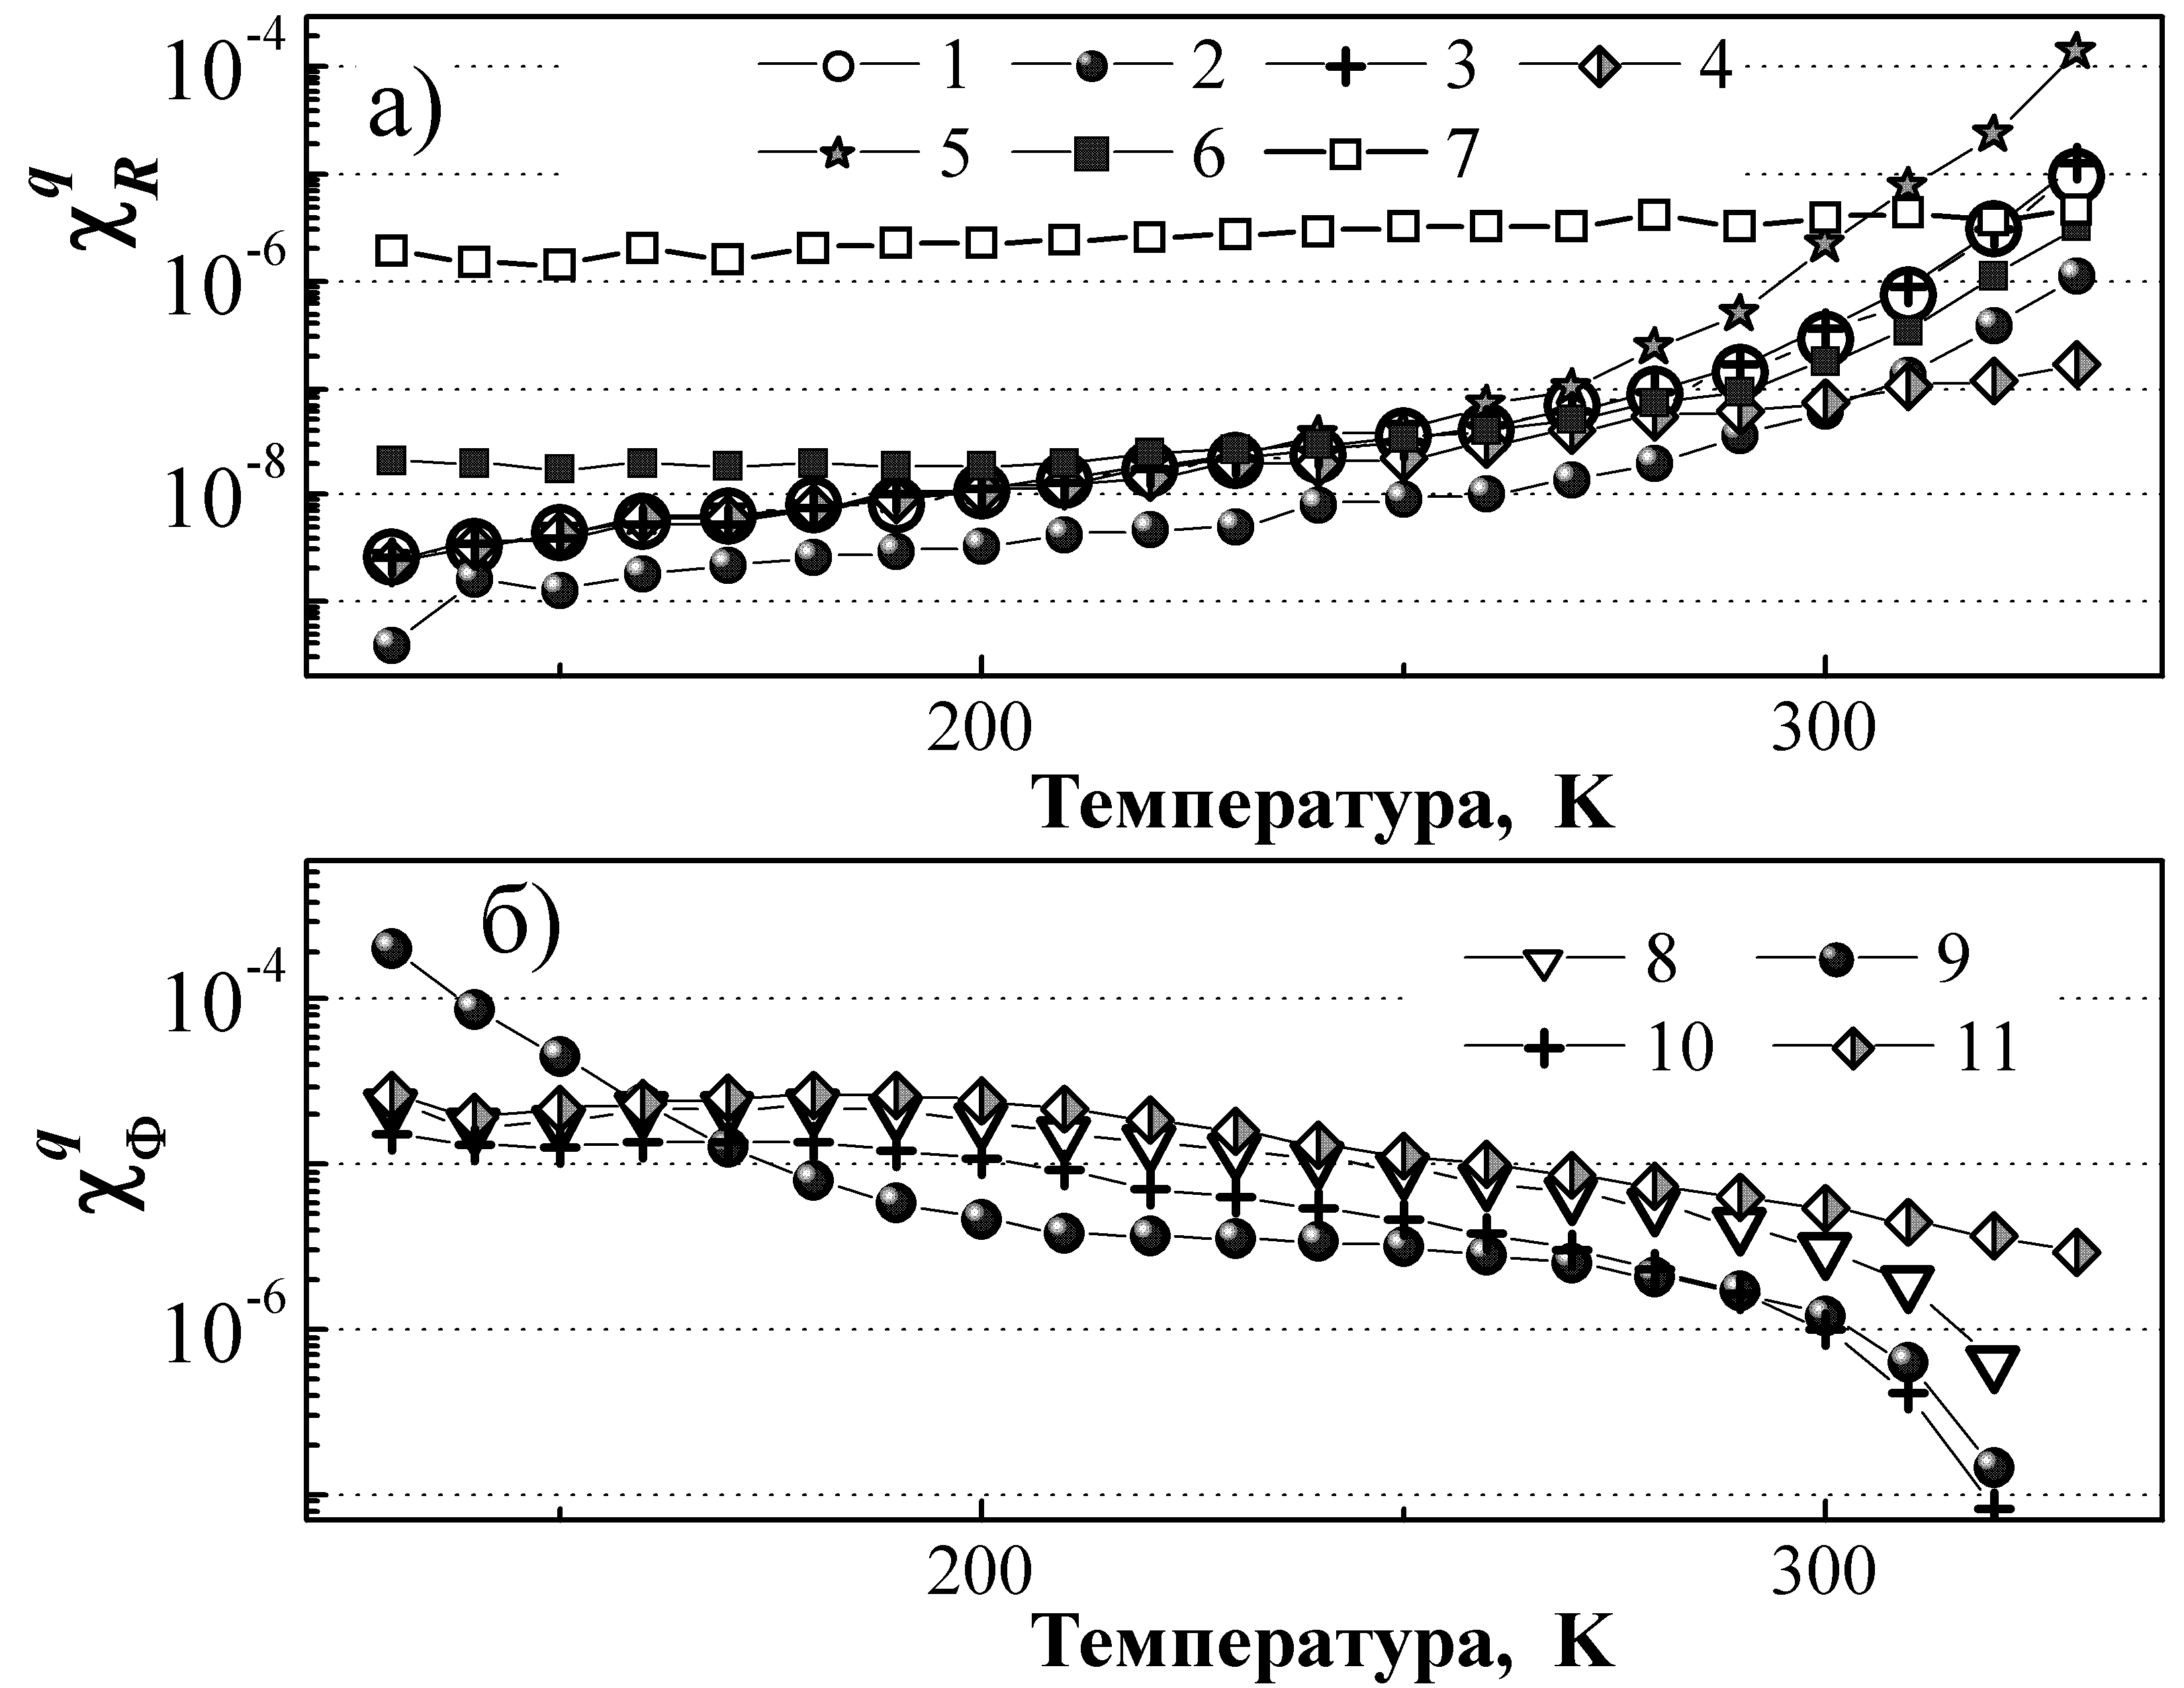
\includegraphics[width=0.9\textwidth]{figCon}%
\caption{\label{figCon}
Температурні залежності точності визначення $R_s$ (a) та $\Phi_b$ (б) при використанні методів Gromov (a) та  Kaminskii I (б).
Під час синтезу ВАХ використовувалися параметри, величини яких переважно визначались формулами~(\ref{eqSDIs}--\ref{eqRsT}),
проте для  побудови кривих 2 та 9 використовувалися ВАХ для яких значення $R_s$ було в 3 рази більше,
для кривих 3 та 10 величина $n_\mathrm{id}$ була в 1,2 рази більша,
для кривих 4 та 11 величина $I_s$ була в 100 разів менша,
для кривої 5 значення $\Phi_b$ було зменшено на 0,1 еВ,
для кривої 6 величини $R_s$ та $\Phi_b$ залишалися незмінними та рівними 2~Ом та 0,7~еВ, відповідно, під час синтезу всього
набору ВАХ (були незалежні від температури),
для кривої 7 значення $R_s$ та $I_s$ були незмінні та рівні 2~Ом та $10^{-5}$~A, відповідно.
}
\end{figure}

З іншого боку, наведені результати показують, що точність визначення параметрів змінюється для різних ВАХ з одного набору (залежить від температури, при якій ВАХ була синтезована).
Фактично мова йде про те, що похибка визначення параметру з масиву $\left\{R_s\,,\,n_\mathrm{id}\,,\, I_s\right\}$ залежить як від його величини, так і від значення інших характеристик ДШ з цього набору.
Для виявлення подібних залежностей всі методи були також застосовані до синтезованих даних, при створенні яких вважалося, що одна з величин з набору ($R_s$, $\Phi_b$, $I_s$ $n_\mathrm{id}$) відрізняється за значенням від того, який очікується згідно з виразами ~(\ref{eqSDIs}--\ref{eqRsT}).
Деякі характерні результати наведені на Рис.~\ref{figCon}.

Рис.~\ref{figCon},a показує що, похибки визначення послідовного опору при використанні методу Gromov
\begin{enumerate}[label=\asbuk*),leftmargin=0em,itemindent=1.5em]
\item зростають з підвищенням $\Phi_b$;
\item зменшуються при збільшенні $R_s$ та зменшенні $I_s$;
\item залишаються практично постійними при зміні $n_\mathrm{id}$.
\end{enumerate}
Очевидно, що $I_s$ та $\Phi_b$ пов'язані між собою співвідношенням~(\ref{eqSDIs}).
Проте, на нашу думку, саме величина струму насичення, а не ВБШ, є першочерговим фактором впливу на процес визначення $R_s$.
На користь цього висновку свідчать криві 6 та 7 на Рис.~\ref{figCon},a.
Так, крива 6 була отримана для набору ВАХ, які синтезовані використовуючи припущення що незалежними від температури є як $R_s$, так і $\Phi_b$.
Незважаючи на ці обмеження, $\chi^q_R$ зростає при збільшенні температури.
На противагу, крива 7, отримана для незалежних від температури $R_s$ та $I_s$, показує, що точність визначення послідовного опору залишається практично постійною для всього набору ВАХ.
З іншого боку, Рис.~\ref{figCon},б показує, що при використанні методу Kaminskii I зменшення струму насичення підвищує похибку визначення ВБШ.
Загалом проведені дослідження показують, що величина $I_s$ є основним, а величина  $\Phi_b$ другорядним визначальними факторами для точності екстракції інших параметрів (не лише $R_s$) при використанні різних методів (не лише Gromov).
З Рис.~\ref{figCon},б також видно, що похибка визначення $\Phi_b$ зменшується у випадку більших значень фактору неідеальності (криві 8 та 10).
В той же час збільшення послідовного опору немонотонно впливає на точність екстракції ВБШ (криві 8 та 9 на Рис.~\ref{figCon},б):
при низьких температурах (високих значеннях $\Phi_b$) $\chi^q_{\Phi}$ зростає, при високих $T$ --- навпаки, зменшується.

Узагальнюючи аналіз отриманих результатів, можна зробити висновок, що точність визначення кожного з параметрів як правило зростає зі збільшенням його величини.
Проте, точність визначення $\chi^q_{x_i}$ даного параметру ($x_i\in\left\{R_s\,,\,n_\mathrm{id}\,,\, I_s\right\}$) залежить також і від абсолютних величин інших характеристик ДШ ($x_j,\,j\neq i$), причому характер цих залежностей є функцією абсолютних значень кожного параметру з набору і змінюється при використанні різних методів ($\chi^q_{x_i}=f(x_i,\,x_j,\,\text{метод})$).


\begin{figure}
\center
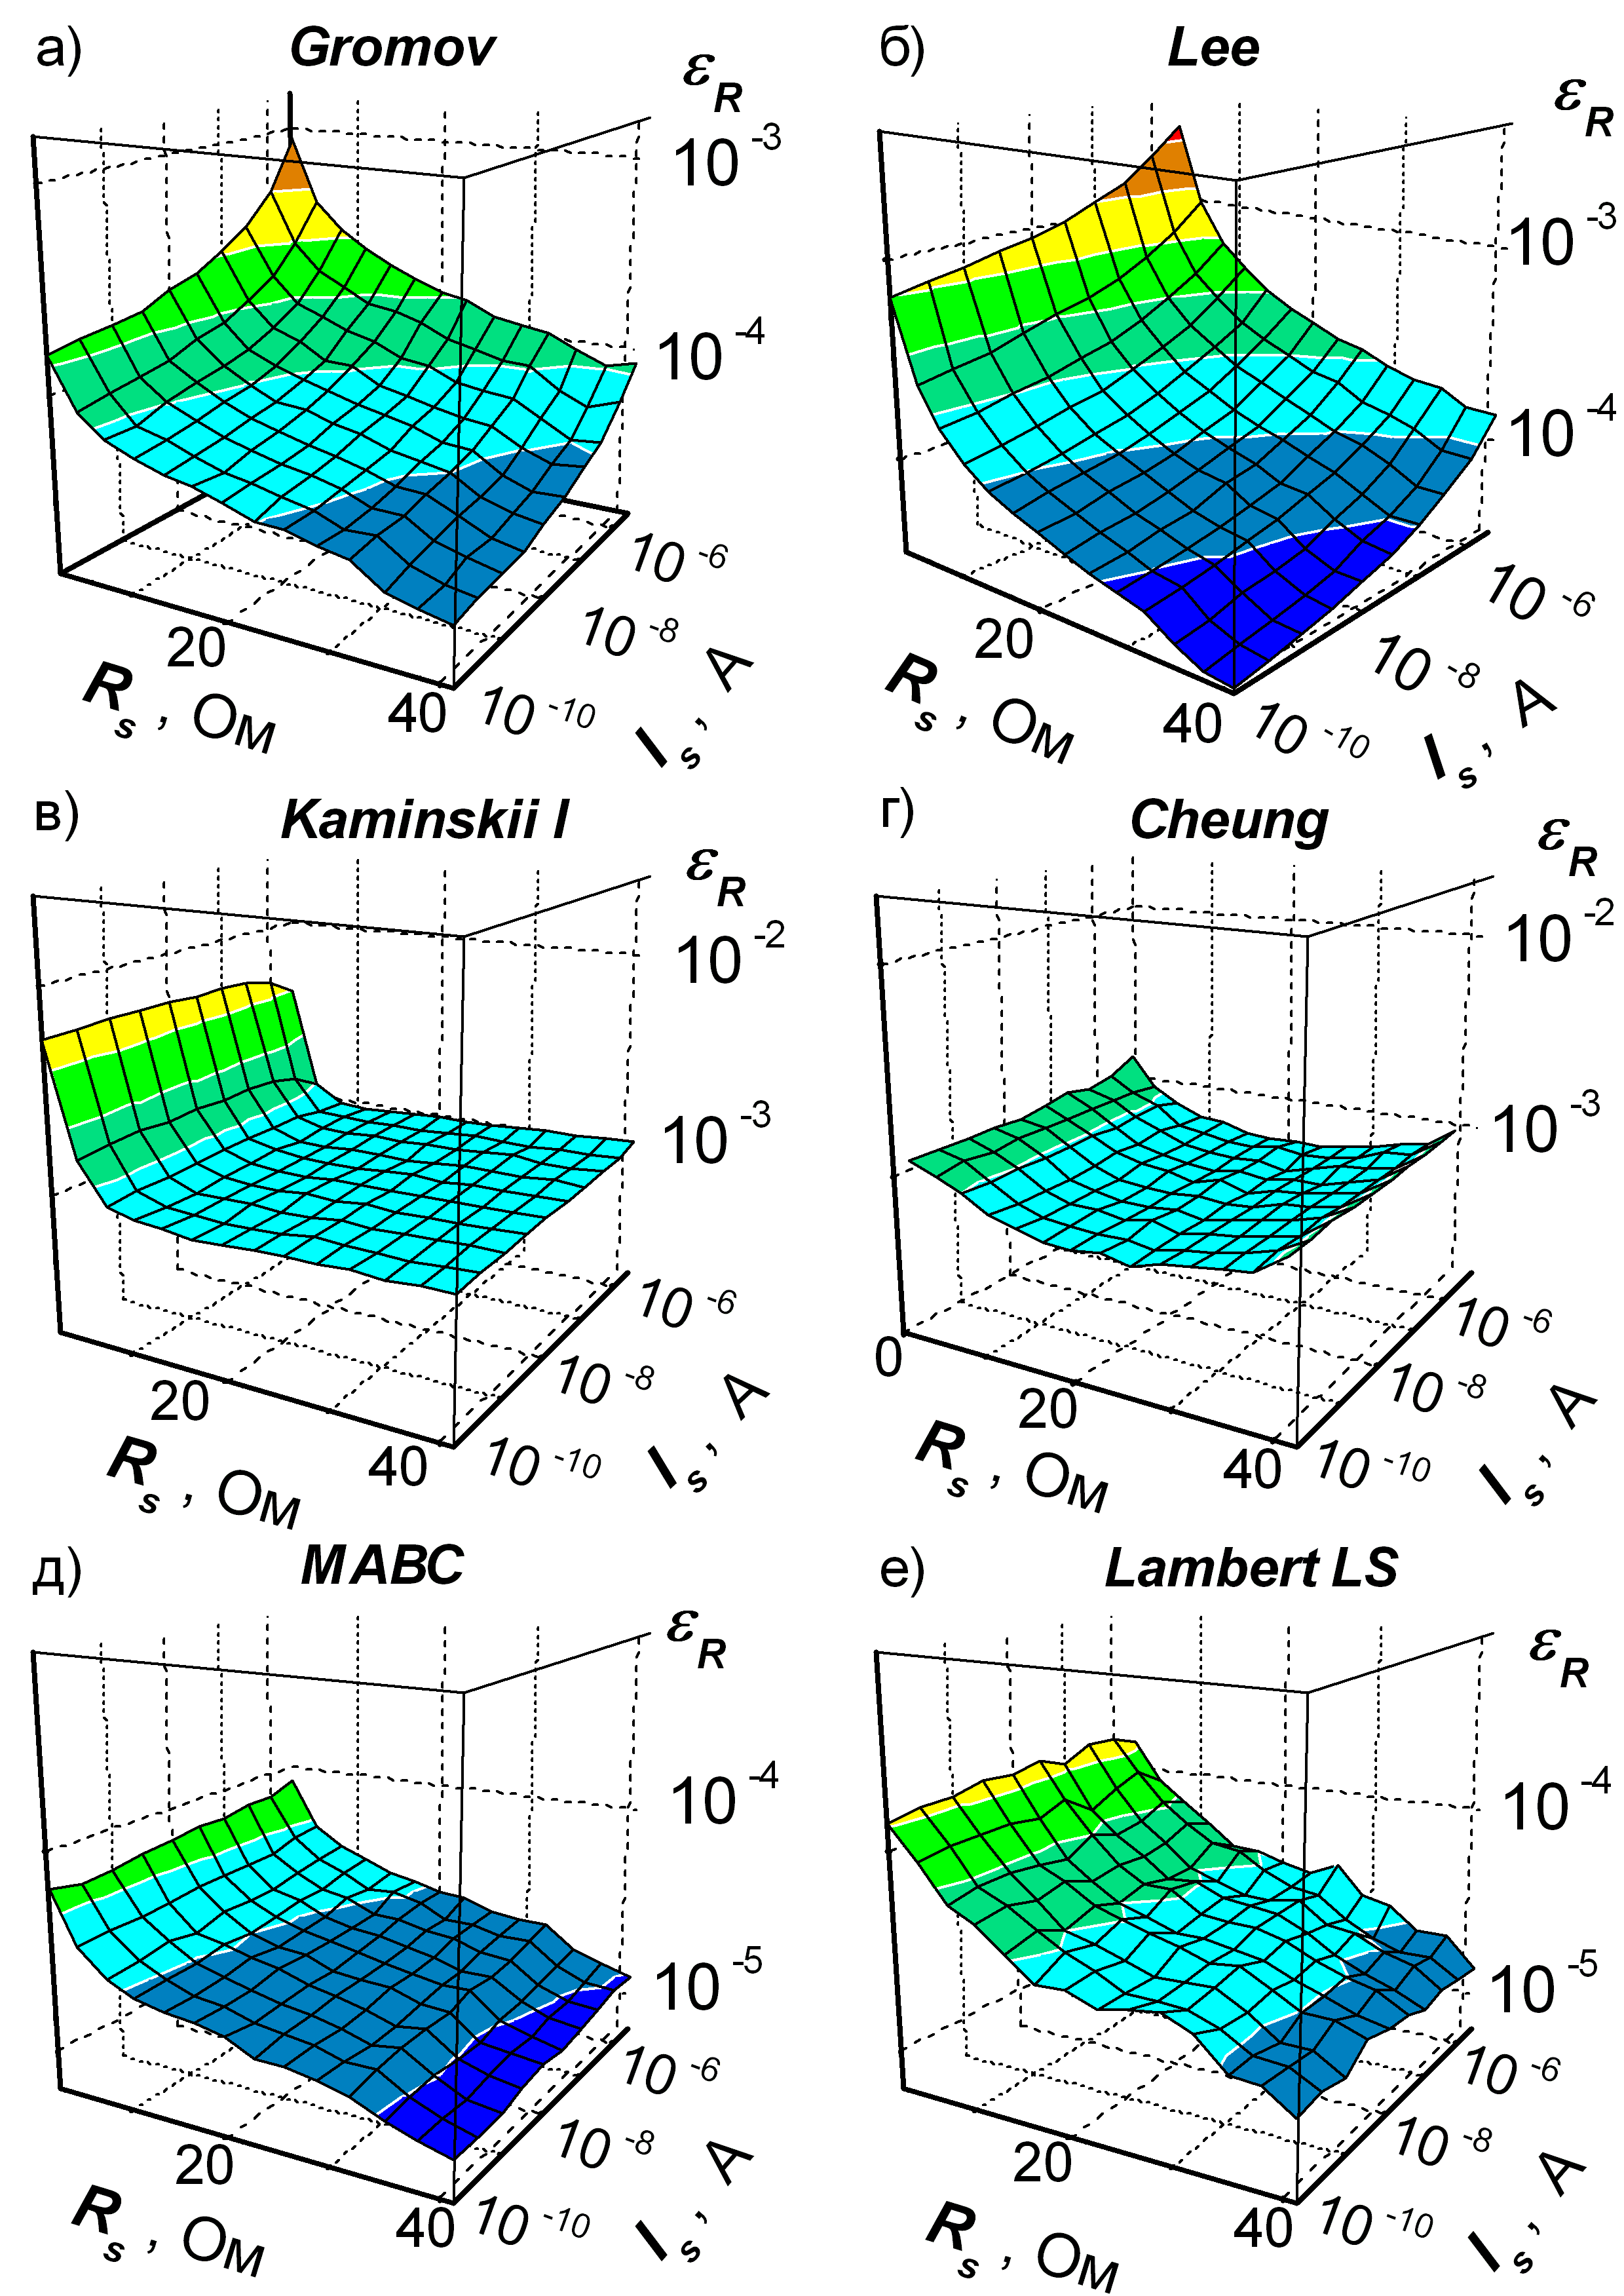
\includegraphics[width=0.9\textwidth]{figR3D}%
\caption{\label{figR3D}
Точність визначення величини послідовного опору з набору ВАХ, який був синтезований при постійних значеннях $R_s$ та $I_s$.
Показані результати застосування методів Gromov (a), Lee (б), Kaminskii I (в), Cheung (г), MABC (д) та and Lambert LS (е).
}
\end{figure}

\begin{figure}
\center
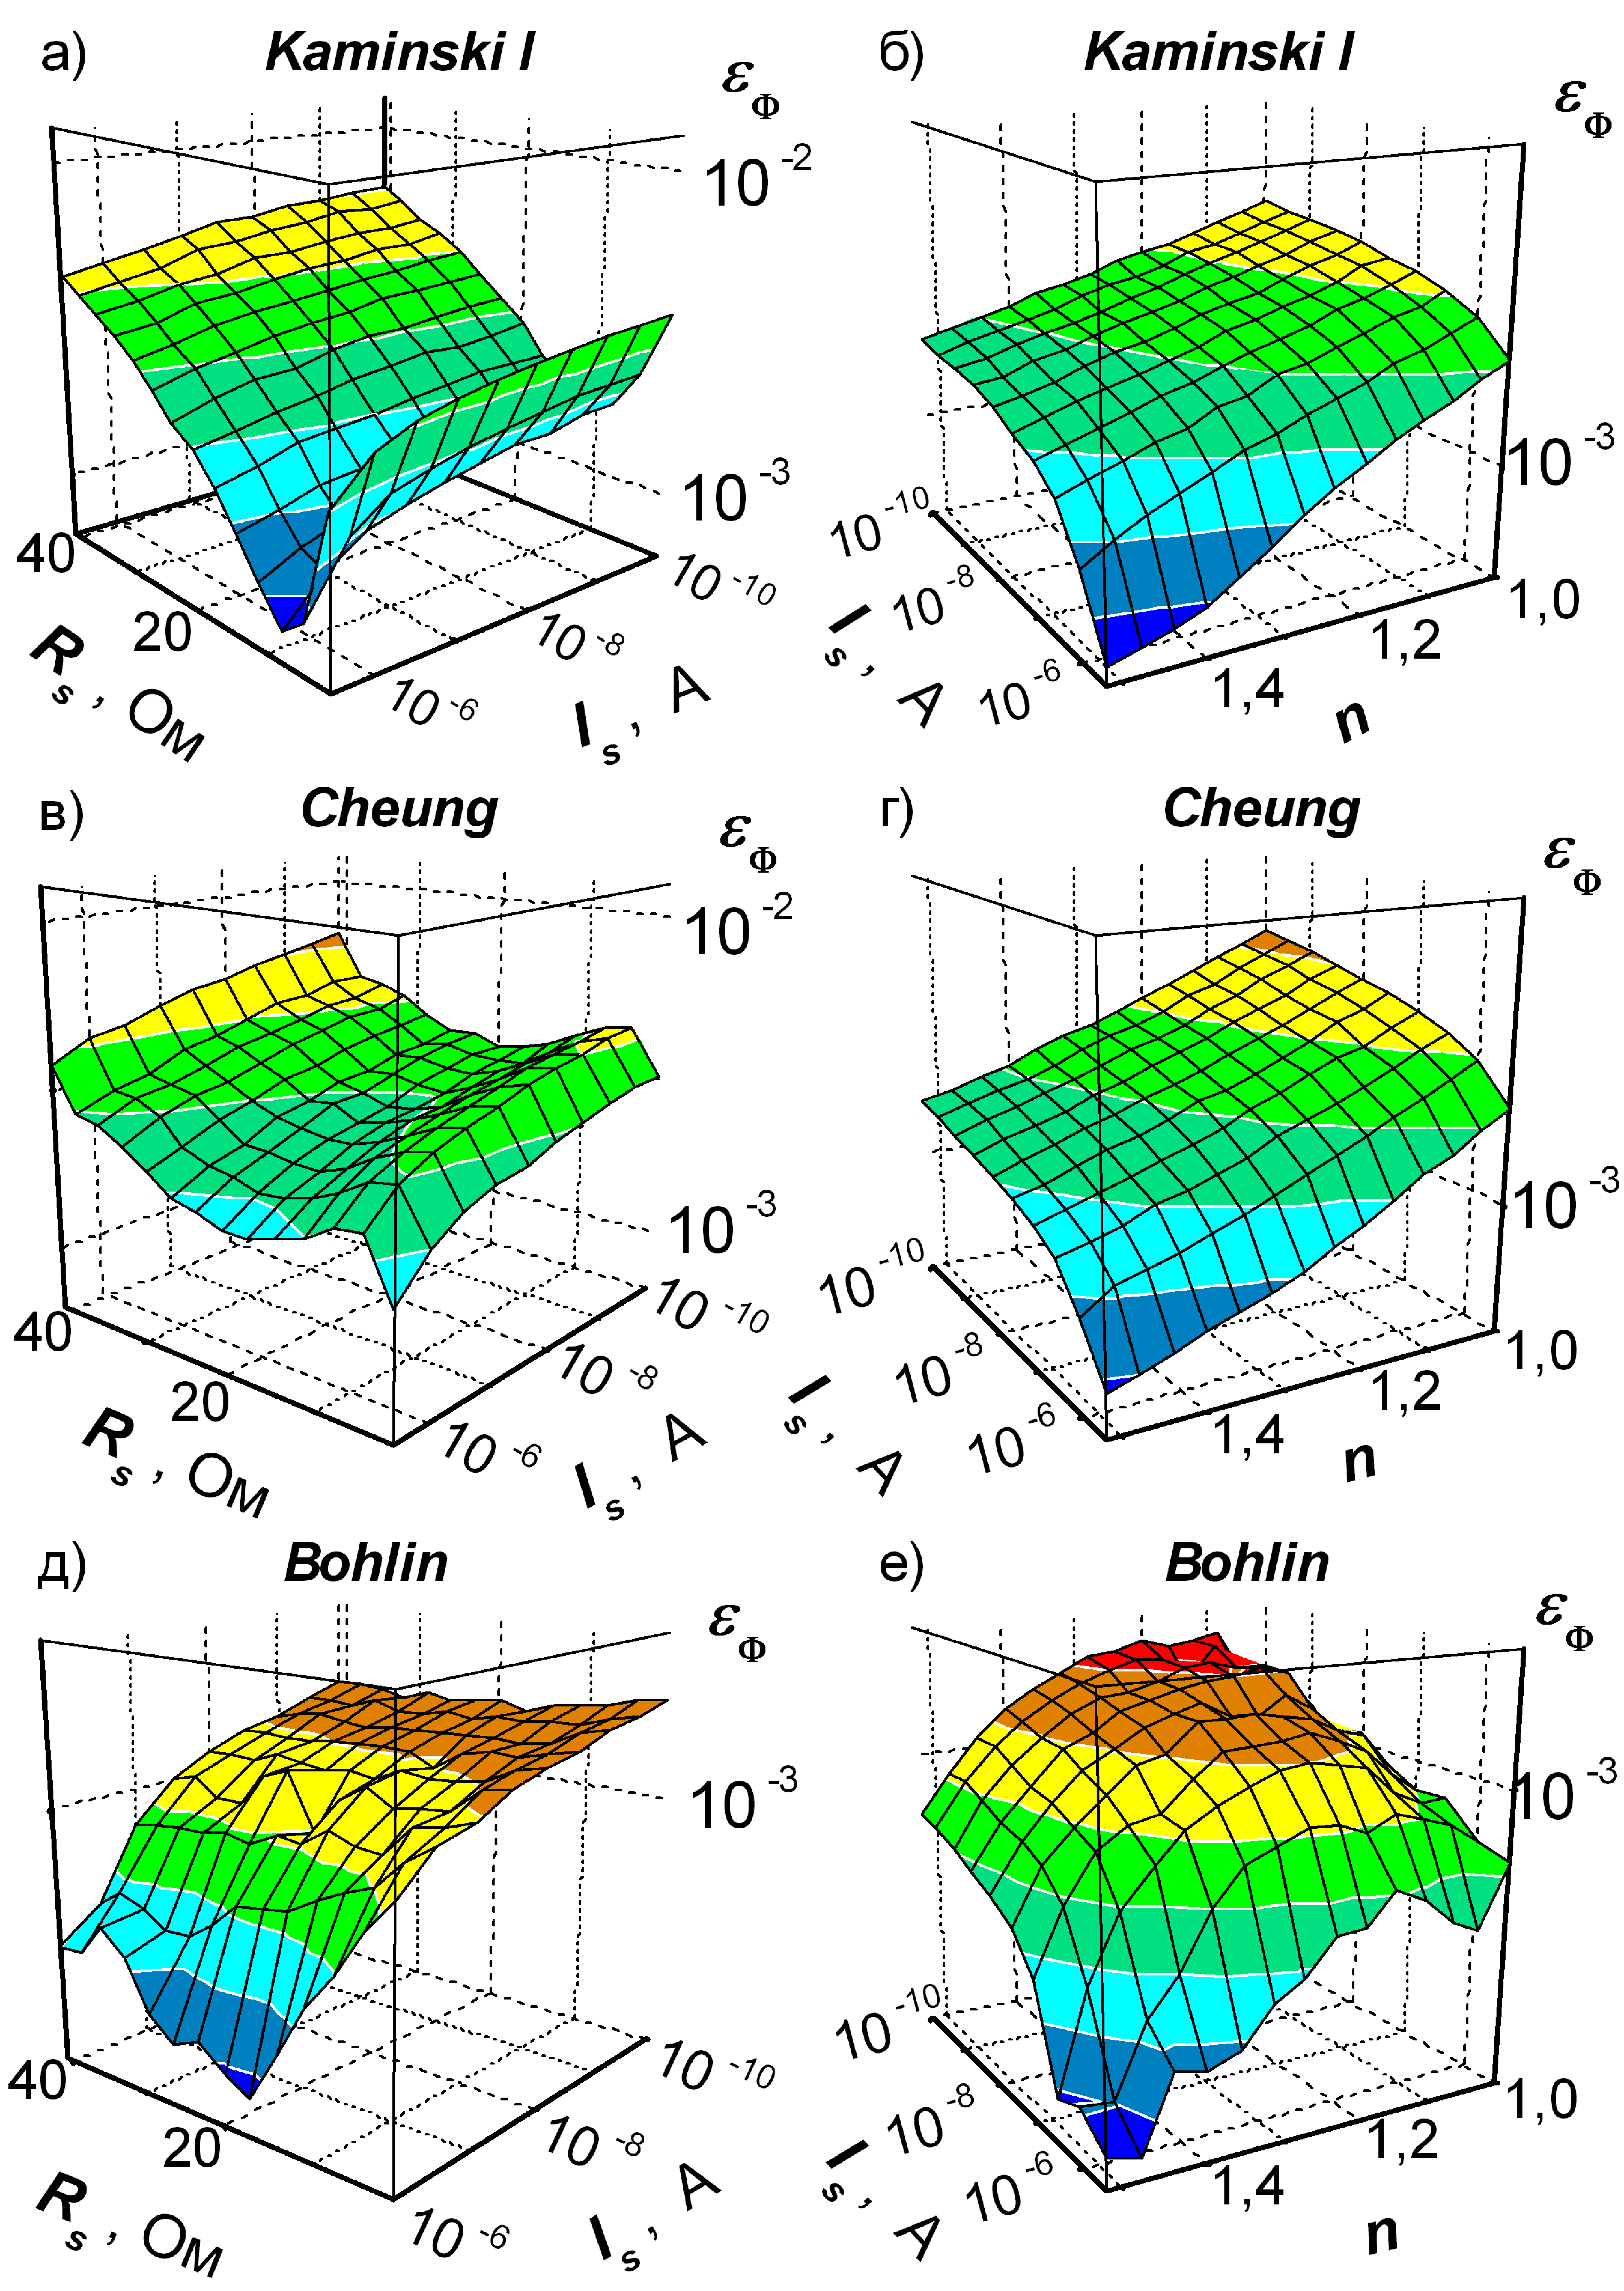
\includegraphics[width=0.9\textwidth]{figF3D}%
\caption{\label{figF3D}
Точність визначення величини висоти бар'єру Шотки опору з набору ВАХ, який був синтезований при постійних значеннях $R_s$ та $I_s$ (рисунки а, в та д) або постійних значеннях $n_\mathrm{id}$ та $I_s$ (рисунки б, г, е).
Показані результати застосування методів Kaminskii I (a, б), Cheung (в, г) та Bohlin (д, е).
}
\end{figure}


\begin{figure}
\center
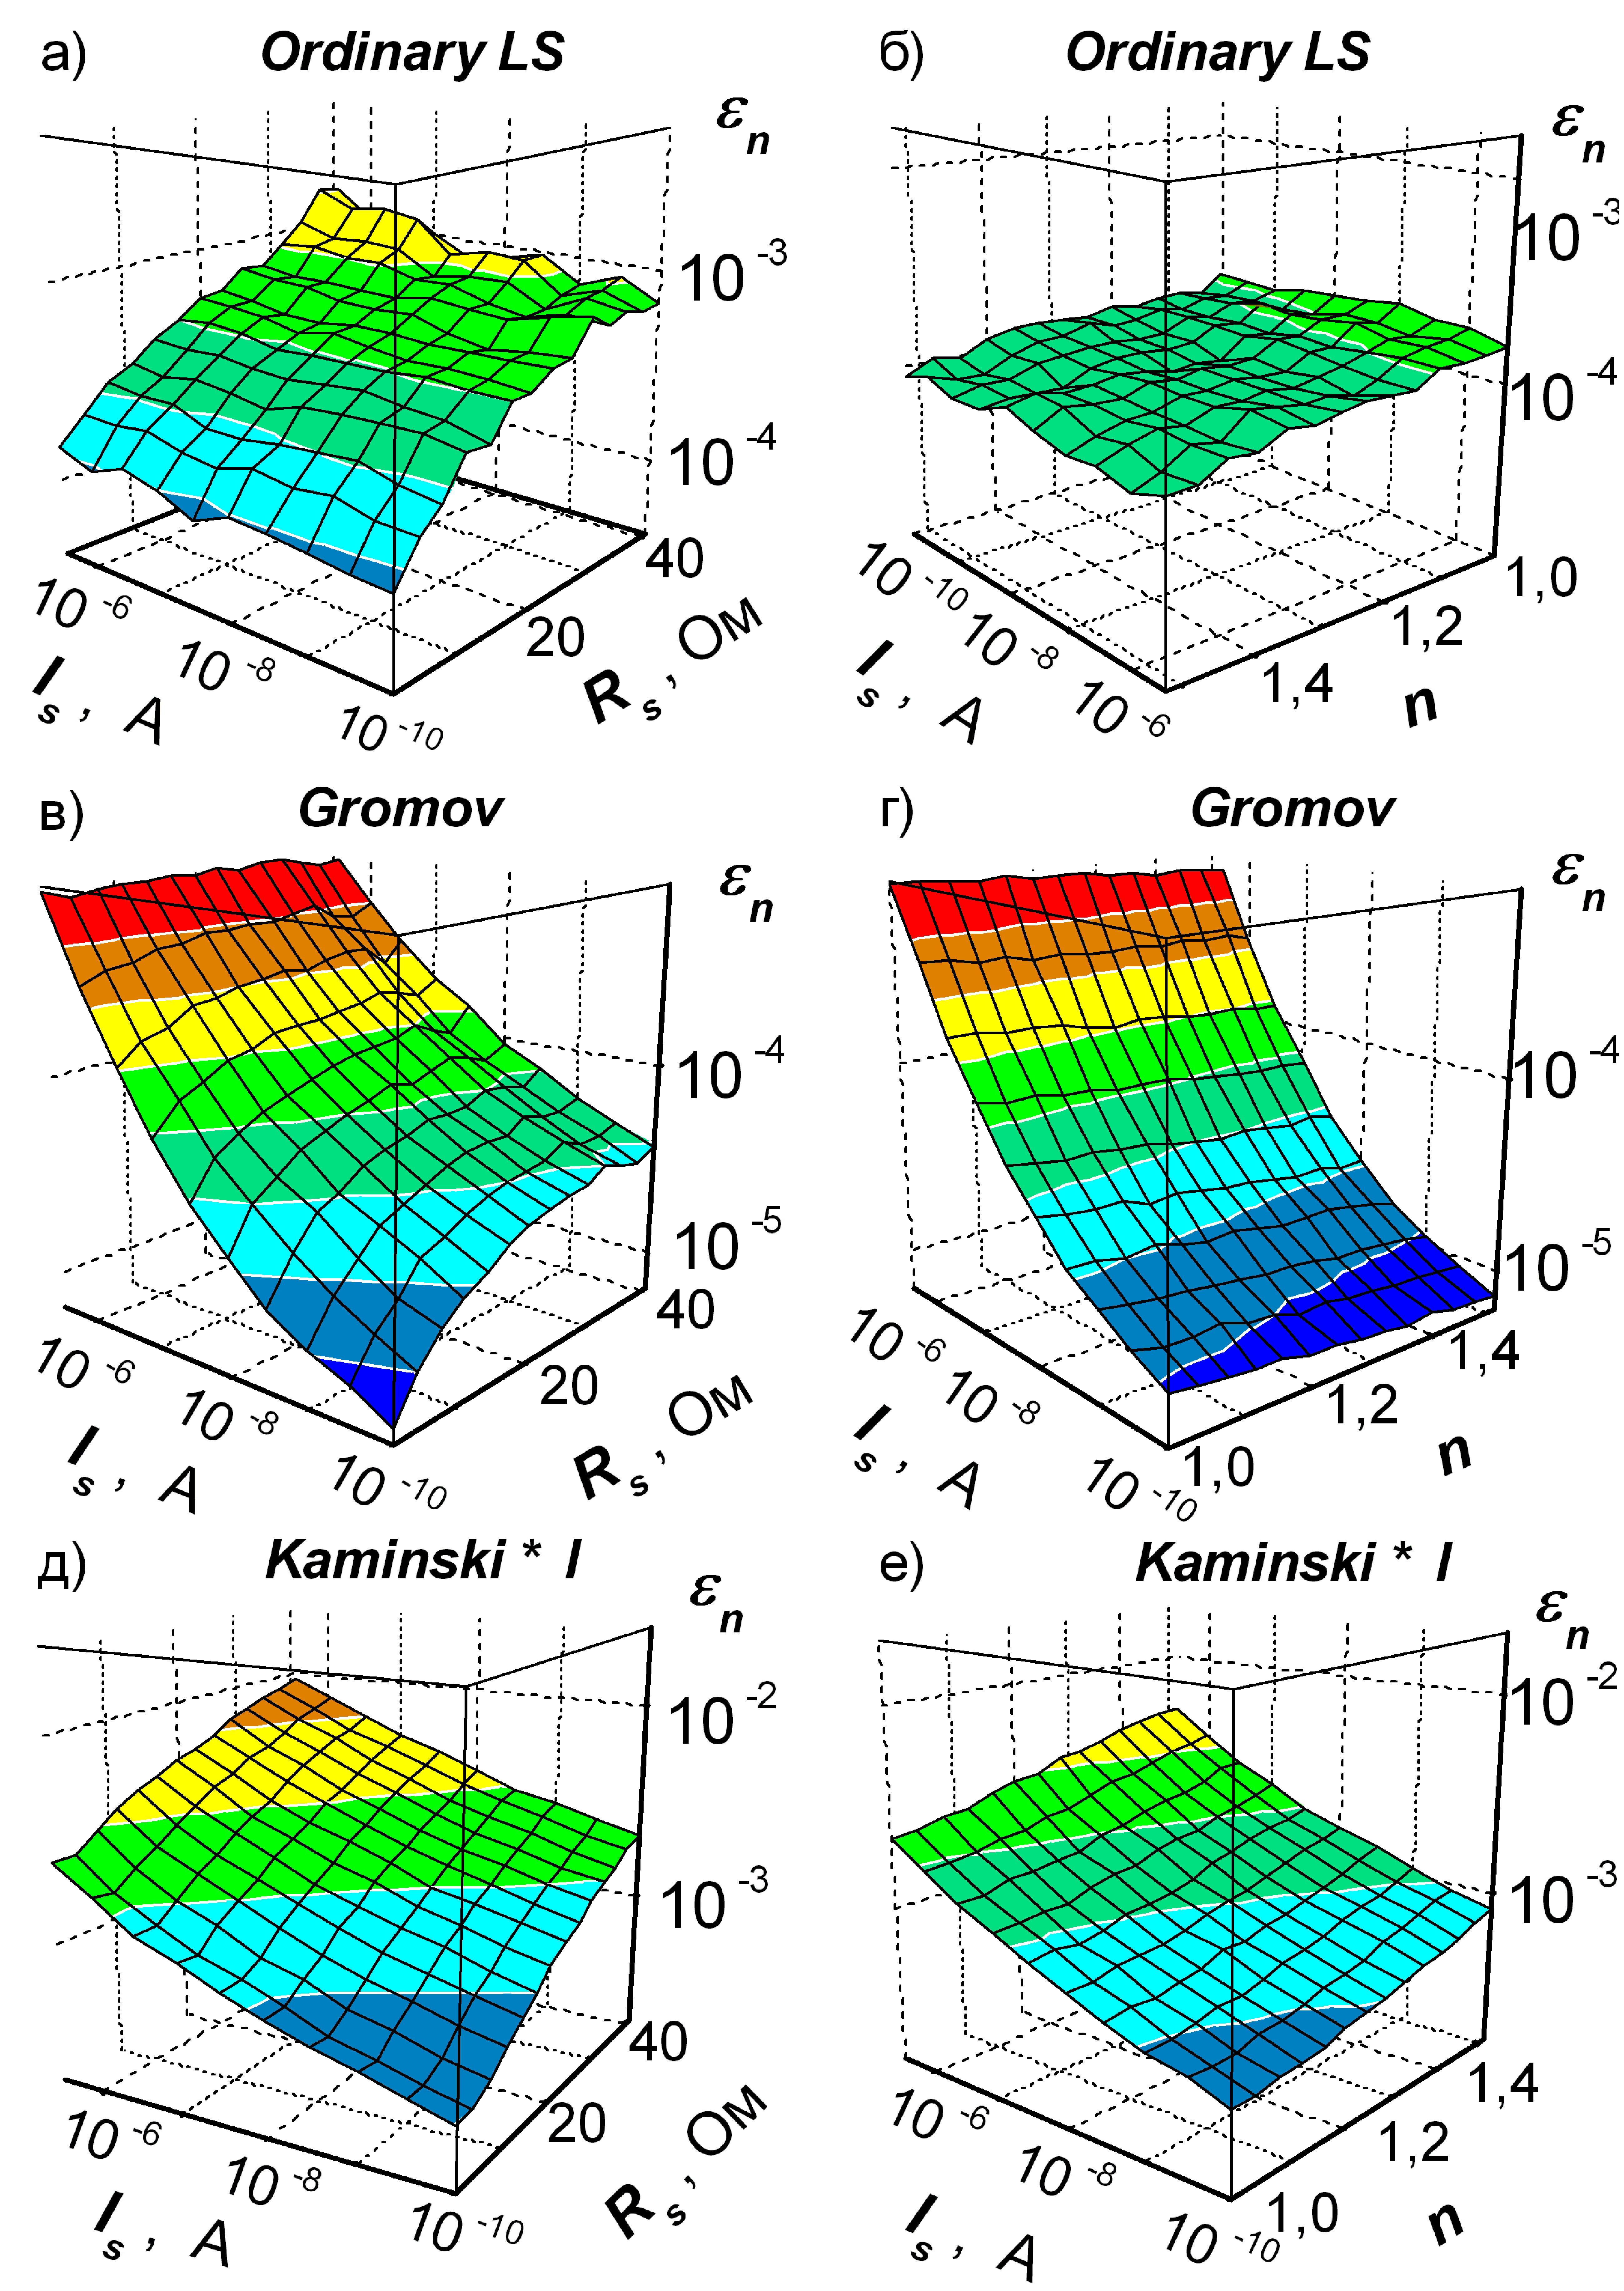
\includegraphics[width=0.9\textwidth]{fign3D}%
\caption{\label{fign3D}
Точність визначення величини фактору неідеальності з набору ВАХ, який був синтезований при постійних значеннях $R_s$ та $I_s$ (рисунки а, в та д) або постійних значеннях $n_\mathrm{id}$ та $I_s$ (рисунки б, г, е).
Показані результати застосування методів Ordinary LS (a, б), Gromov (в, г) та Kaminskii*~I (д, е).
}
\end{figure}

Для того, щоб виявити основні тенденції цих залежностей були проведені додаткові дослідження.
А саме, були синтезовані набори ВАХ, при побудові яких вважалося, що деякі параметри є незалежними від температури.
В цьому випадку
а)~постійними у всьому температурному діапазоні вважалася два параметри ($R_s$ та $I_s$  або $n_\mathrm{id}$ та $I_s$ для різних наборів ВАХ);
б)~$n_\mathrm{id}$ (або $R_s$) розраховувалися відповідно до того, як описано раніше, в розділі~\ref{SubData}.
Було створено сукупність наборів ВАХ, для яких незалежні від температури величини $R_s$, $n_\mathrm{id}$ та $I_s$ змінювались в діапазонах від
2 до 41~Ом, від 1 до 1,52 та від $10^{-10}$ до $5\cdot10^{-5}$~A, відповідно.
Після цього кожен з методів було застосована до кожного з набору ВАХ, визначено величини параметрів, а також їх похибки.
Найбільш типові результати наведено ни Рис.~\ref{figR3D}--\ref{fign3D}.
Зокрема, Рис.~\ref{figR3D},a підтверджує, що при використанні методу Gromov збільшення $R_s$ та $I_s$ призводить до зменшення та збільшення помилки визначення послідовного опору, відповідно.


Отримані результати щодо факторів впливу узагальнено в Таблиці~\ref{tabIF}.
В цій таблиці використано ряд символів для опису поведінки точності визначення параметрів при зміні величини фактору впливу.
А саме.
Якщо помилка визначення монотонно зростає або зменшується зі збільшенням впливаючого фактору, то використовувались символи <<$\downarrow$>> та <<$\uparrow$>>, відповідно.
Наприклад, саме ці символи характеризують кореляцію точності визначення $R_s$ за допомогою методу Gromov та величини $R_s$ та $I_s$.



\begin{table}
\caption{\label{tabIF}Фактори впливу на точність визначення параметрів ДШ.$^{1)}$
%\footnote{The presence of $R_s$ or $I_s$ or $n$ in the cell indicates the impact on extracted parameter accuracy;
%the subscript and inside bracket symbol deal with extraction error behavior with influencing factor increasing --- see details in the text.}
}
\begin{tabular}{|l|c|c|c|}
%\begin{tabularx}{\textwidth}{|l|
%                              >{\centering\arraybackslash}X|
 %                             >{\centering\arraybackslash}X|
  %                            >{\centering\arraybackslash}X|}
\hline
\multicolumn{1}{|c|}{Метод}&\multicolumn{3}{c|}{Визначений параметр}\\
\cline{2-4}
%\hline
 &$R_s$&$\Phi_b$&$n$\\
%Метод &$R_s$&$\Phi_b$&$n$\\
%\hline
%\hline
\hhline{|====|}
Norde &$n_\mathrm{id}^w(\vee)$&$I_s(\downarrow)$&---\\
\hline
Werner &$R_s(\vee)$&$R_s(\downarrow)$, $I_s^w(\downarrow)$, $n_\mathrm{id}^w(\downarrow)$&$R_s(\uparrow)$, $n_\mathrm{id}^w(\downarrow)$\\
\hline
Werner* &$R_s(\vee)$&$R_s(\vee)$, $I_s(\uparrow)$, $n_\mathrm{id}(\uparrow)$&$R_s(\vee)$, $I_s(\uparrow)$, $n_\mathrm{id}^w(\uparrow)$\\
\hline
Cibils &$R_s(\vee)$, $n_\mathrm{id}(\uparrow)$&$R_s(\uparrow)$, $n_\mathrm{id}(\vee)$& $R_s(\uparrow)$, $n_\mathrm{id}(\vee)$\\
\hline
Cibils* &$R_s(\vee)$, $n_\mathrm{id}(\uparrow)$&$R_s(\vee)$, $I_s(\uparrow)$, $n_\mathrm{id}(\uparrow)$& $R_s(\vee)$, $I_s(\uparrow)$, $n_\mathrm{id}(\uparrow)$\\
\hline
Kaminskii I&$R_s(\leftharpoonup)$, $n_\mathrm{id}^w(\downarrow)$&$R_s(\vee)$, $I_s(\downarrow)$, $n_\mathrm{id}(\downarrow)$& $R_s(\vee)$, $I_s^w(\downarrow)$, $n_\mathrm{id}(\downarrow)$\\
\hline
Kaminskii* I&$R_s(\leftharpoonup)$, $n_\mathrm{id}^w(\downarrow)$&$R_s(\uparrow)$, $I_s(\uparrow)$, $n_\mathrm{id}(\uparrow)$& $R_s(\uparrow)$, $I_s(\uparrow)$, $n_\mathrm{id}(\uparrow)$\\
\hline
Kaminskii II&$R_s(\downarrow)$, $I_s(\rightharpoonup)$, $n_\mathrm{id}^w(\uparrow)$&$I_s(\rightharpoonup)$, $n_\mathrm{id}^w(\uparrow)$& $I_s(\rightharpoonup)$\\
\hline
Kaminskii* II&$R_s(\downarrow)$, $I_s(\rightharpoonup)$, $n_\mathrm{id}^w(\uparrow)$&$I_s(\uparrow)$, $n_\mathrm{id}(\uparrow)$& $I_s(\uparrow)$, $n_\mathrm{id}(\uparrow)$\\
\hline
Bohlin &$I_s(\rightharpoondown)$&$I_s(\downarrow)$, $n_\mathrm{id}(\wedge)$& $I_s(\rightharpoondown)$, $n_\mathrm{id}(\wedge)$\\
\hline
Lee &$R_s(\downarrow)$, $I_s(\uparrow)$, $n_\mathrm{id}(\uparrow)$&$I_s(\uparrow)$, $n_\mathrm{id}(\uparrow)$& $I_s(\uparrow)$, $n_\mathrm{id}(\uparrow)$\\
\hline
Gromov &$R_s(\downarrow)$, $I_s(\uparrow)$&$R_s(\uparrow)$, $I_s(\uparrow)$, $n_\mathrm{id}^w(\downarrow)$&$R_s(\uparrow)$, $I_s(\uparrow)$, $n_\mathrm{id}^w(\downarrow)$\\
\hline
Cheung &$R_s^w(\vee)$&$R_s(N)$, $I_s(\downarrow)$, $n_\mathrm{id}(\downarrow)$&$R_s^w(N)$, $I_s(\rightharpoondown)$, $n_\mathrm{id}(\downarrow)$\\
\hline
Mikhelashvili &$R_s(\uparrow)$, $I_s(\downarrow)$, $n_\mathrm{id}^w(\downarrow)$&$R_s(\uparrow)$, $I_s(\wedge)$, $n_\mathrm{id}^w(\downarrow)$&$R_s(\uparrow)$, $I_s(\wedge)$, $n_\mathrm{id}^w(\downarrow)$\\
\hline
Ordinary LS &$R_s(\downarrow)$&$R_s(\uparrow)$, $I_s^w(\downarrow)$, $n_\mathrm{id}^w(\downarrow)$&$R_s(\uparrow)$, $n_\mathrm{id}^w(\downarrow)$\\
\hline
Lambert LS &$R_s(\downarrow)$&$I_s^w(\downarrow)$&$n_\mathrm{id}^w(\downarrow)$\\
\hline
EAs &$R_s(\downarrow)$, $I_s^w(\uparrow)$&$R_s(\uparrow)$, $I_s(\vee)$, $n_\mathrm{id}^w(\downarrow)$&$R_s(\uparrow)$, $I_s(\vee)$, $n_\mathrm{id}^w(\downarrow)$\\
\hline
\multicolumn{4}{|p{\textwidth}|}{$^{1}$\textit{Наявність $R_s$ або $I_s$ або $n_\mathrm{id}$ в клітинці означає
вплив величини, відповідно, послідовного опору або струму насичення або фактору неідеальності на точність визначення параметру;
верхній індекс та символ в дужках пов'язані з характером поведінки точності визначення параметру при збільшенні $R_s$ або $I_s$ або $n_\mathrm{id}$ --- деталі див. у тексті.
}}\\
\hline
\end{tabular}
%\end{tabularx}
\end{table}

Виявлено, може залежати від фактору впливу не лише монотонно.
Наприклад, Рис.~\ref{figCon},б та Рис.~\ref{figF3D},a показують, що при використанні методу Kaminskii~I похибка визначення $\Phi_b$ зростає з підвищенням послідовного опору при великих ($>10$~Ом) значеннях $R_s$ і зменшується при малих величинах $R_s$.
Для позначення залежності з такою поведінкою в Таблиці~\ref{tabIF} використовується символ <<$\vee$>>.
Подібна залежність спостерігається при використанні метода Chueng для визначення $R_s$ --- див. Рис.~\ref{figR3D},г.
Проте в цьому випадку сама величина $R_s$ порівняно слабко впливає на точність визначення послідовного опору.
Схожі слабкі залежності позначаються в Таблиці~\ref{tabIF} за допомогою верхнього індексу  <<$w$>>.
Інші приклади слабких залежностей $I_s$ та  $n_\mathrm{id}$ можна побачити на Рис.~\ref{figR3D},д та Рис.~\ref{fign3D},г, відповідно.

Якщо графік залежності точності визначення параметру від величини фактору впливу має не мінімум, а максимум (див., наприклад, Рис.~\ref{figF3D},е),
то використовувався символ <<$\wedge$>>.
Наявність на залежності екстремумів обох типів (див., наприклад, Рис.~\ref{figF3D},в) позначено за допомогою символу <<$N$>>.

Ще один тип залежності показаний на Рис.~\ref{figR3D},в.
При використанні методу Kaminskii~I для визначення  $R_s$ помилки залишаються постійними в широкому діапазоні змін $R_s$ та $I_s$ і зростають лише для малих значень $R_s$.
Подібні залежності між помилкою визначення та впливаючим фактором позначені символом <<$\leftharpoonup$>>.
Символи <<$\rightharpoonup$>> або <<$\rightharpoondown$>> якщо помилки зростають або зменшуються, відповідно, лише при великих значеннях фактору впливу.

З наведених даних, зокрема, видно, що фактори, які впливають на точність екстракції $\Phi_b$ та  $n_\mathrm{id}$ подібні для більшості методів, які розглядалися в роботі.
Використання адаптивної процедури в методі Gromov призводить до того, що точність визначення $\Phi_b$ та  $n_\mathrm{id}$ стає залежною від величини $R_s$, тоді як вплив величини фактору неідеальності послаблюється.
Точність методів Werner*, Cibils* та Kaminskii* більш чутлива до величин параметрів ніж при використанні варіантів цих же методів без зірочок.
Найбільш стійкими до величин параметрів є точності чисельних методів, особливо при використанні функції Ламберта (Lambert LS).


\subsection{Швидкодія методів визначення параметрів ДШ}
Ще одним, поряд з точністю, критерієм для характеризації різних методів визначення параметрів структур МН є час, необхідний для визначення параметрів (RT, running time).
Для оцінки RT були використані WinAPI функції $QueryPerformanceCounter()$ та $QueryPerformanceFrequency()$.
Розрахунки проводились на персональному комп'ютері з наступними характеристиками:
\begin{itemize}
  \item процесор AMD A4-3400 2.7~GHz;
  \item 3072~MB RAM;
  \item операційна система Windows XP.
\end{itemize}
Очевидно, що точний час екстракції параметрів залежить від програмної реалізації, від завантаження процесору в даний момент часу тощо.
Тим не менш, всі методи тестувалися за однакових умов, а отже вибраний підхід дозволяє порівняти тривалість роботи різних методів, а також оцінити порядок величини RT.

\begin{table}
\caption{\label{tabRT}Час визначення параметрів ДШ з однієї ВАХ.}
\begin{tabularx}{\textwidth}{|>{\raggedright\arraybackslash}X|
                             >{\centering\arraybackslash}X|
                            >{\centering\arraybackslash}X|}
\hline
\multicolumn{1}{|c|}{Метод}&\multicolumn{2}{c|}{Час роботи, с}\\
\cline{2-3}
%\begin{tabular}{lcc}
%Method &\multicolumn{2}{c}{Running time, s}\\
 &максимальний&мінімальний\\
\hhline{|===|}
Norde &$3.7\cdot10^{-5}$&$2.6\cdot10^{-5}$\\ \hline
Werner $^{1)}$ &$4.5\cdot10^{-5}$&$4.0\cdot10^{-5}$\\ \hline
Cibils $^{1)}$ &$5.3\cdot10^{-3}$&$1.9\cdot10^{-4}$\\ \hline
Kaminskii I $^{1)}$ &$8.0\cdot10^{-5}$&$4.5\cdot10^{-5}$\\ \hline
Kaminskii II $^{1)}$ &$2.6\cdot10^{-3}$&$3.0\cdot10^{-4}$\\ \hline
Bohlin &$6.3\cdot10^{-5}$&$4.0\cdot10^{-5}$\\ \hline
Lee &$3.6\cdot10^{-3}$&$1.8\cdot10^{-4}$\\ \hline
Gromov &$2.2\cdot10^{-2}$&$2.2\cdot10^{-2}$\\ \hline
Gromov $^{2)}$ &$4.6\cdot10^{-5}$&$2.7\cdot10^{-5}$\\ \hline
Cheung &$3.2\cdot10^{-5}$&$2.0\cdot10^{-5}$\\ \hline
Mikhelashvili &$4.7\cdot10^{-5}$&$2.9\cdot10^{-5}$\\ \hline
Ordinary LS &$460$&$1.8$\\ \hline
Lambert LS &$540$&$7.6$\\ \hline
DE &$0.73$&$0.36$\\ \hline
PSO &$0.35$&$0.14$\\ \hline
MABC &$0.20$&$5.7\cdot10^{-2}$\\ \hline
TLBO &$19.2$&$5.4$ \\
\hline
\multicolumn{3}{|p{17cm}|}{$^{1}$\textit{Час корекції ВАХ та лінійної апроксимації дорівнює $1.8\cdot10^{-5}$~с (максимальний) або $1.4\cdot10^{-5}$~с (мінімальний)}.
}\\
\multicolumn{3}{|p{17cm}|}{$^{2}$\textit{Для випадку, коли адаптивна процедура не використовується}.
}\\ \hline
\end{tabularx}
\end{table}

Отримані значення RT при застосуванні різноманітних методів до аналізу ідеальних синтезованих ВАХ наведено в Таблиці~\ref{tabRT}.
Загалом, RT залежить від кількості точок у вихідній залежності;
в таблиці наведено значення, отримані при застосування методів до ВАХ, сгенерованих для температур 130~K та 330~K.
Очевидно, що
\begin{enumerate}[label=\asbuk*),leftmargin=0em,itemindent=1.5em]
\item час роботи аналітичних методів при використанні сучасних комп'ютерів знехтувано малий;
\item у випадку ВАХ з великою кількістю експериментальних точок RT чисельних методів може досягати значних величин;
\item використання функції Ламберта призводить до збільшення часу роботи чисельних методів; однією з причин цього є необхідність використовувати числовий ряд для обчислення значення самої функції;
\item використання адаптивної функції очікувано викликає збільшення необхідного часу на декілька порядків, проте абсолютне значення RT залишається досить малим;
\item серед еволюційних алгоритмів найбільш швидким при визначенні параметрів ДШ є MABC, тоді як найбільш повільним --- TLBO.
\end{enumerate}


Узагальнюючи результати, отримані при дослідженні застосування методів до ідеальних синтезованих ВАХ, зауважимо,
що еволюційні алгоритми видаються найбільш придатними для визначення параметрів ДШ завдяки низькому рівню помилок, помірній чутливості точності до величини параметрів
та допустимому часу роботи.
Поряд з цим, іншими методами, яким також варто надавати перевагу є аналітичний метод Gromov з використанням адаптивної процедури та числовий метод Lambert LS.
Проте, точність визначення параметрів для першого з них суттєво зменшується при високих значеннях струму насичення (високих температурах).
Щодо методу Lambert LS, то його основним недоліком є значний час, потрібний для обчислень.


\subsection{Вплив випадкових похибок на точність визначення параметрів структур МН}

На Рис.~\ref{figG1003} та Рис.~\ref{figDiag} наведено результати застосування різноманітних методів до зашумлених даних.
Цілком очікувано, помилки при екстракції параметрів збільшуються при підвищенні рівня шуму (рівня випадкових помилок вимірювань).
Проте залежності правильності визначення параметрів з однієї ВАХ схожі до отриманих при аналізі ідеальних синтезованих ВАХ.
Як наслідок, фактори впливу на точність також ідентичні, тобто дані Таблиці~\ref{tabIF} цілком застосовні і в цьому випадку.
Крім того, інші характерні особливості методів, виявлені раніше, проявляються і в цьому випадку.
Наприклад, використання функції Ламберта дозволяє досягнути більшої точності чисельних методів при визначенні параметрів ДШ.
Еволюційні алгоритми, методи Gromov та Lee характеризуються найменшими помилками.
З іншого боку, різниця між результатами, отриманими за допомогою методів Gromov та Lee зменшується.
Це свідчить про зниження переваги застосування запропонованої адаптивної процедури з підвищенням рівня випадкових похибок.



\begin{figure}
\center
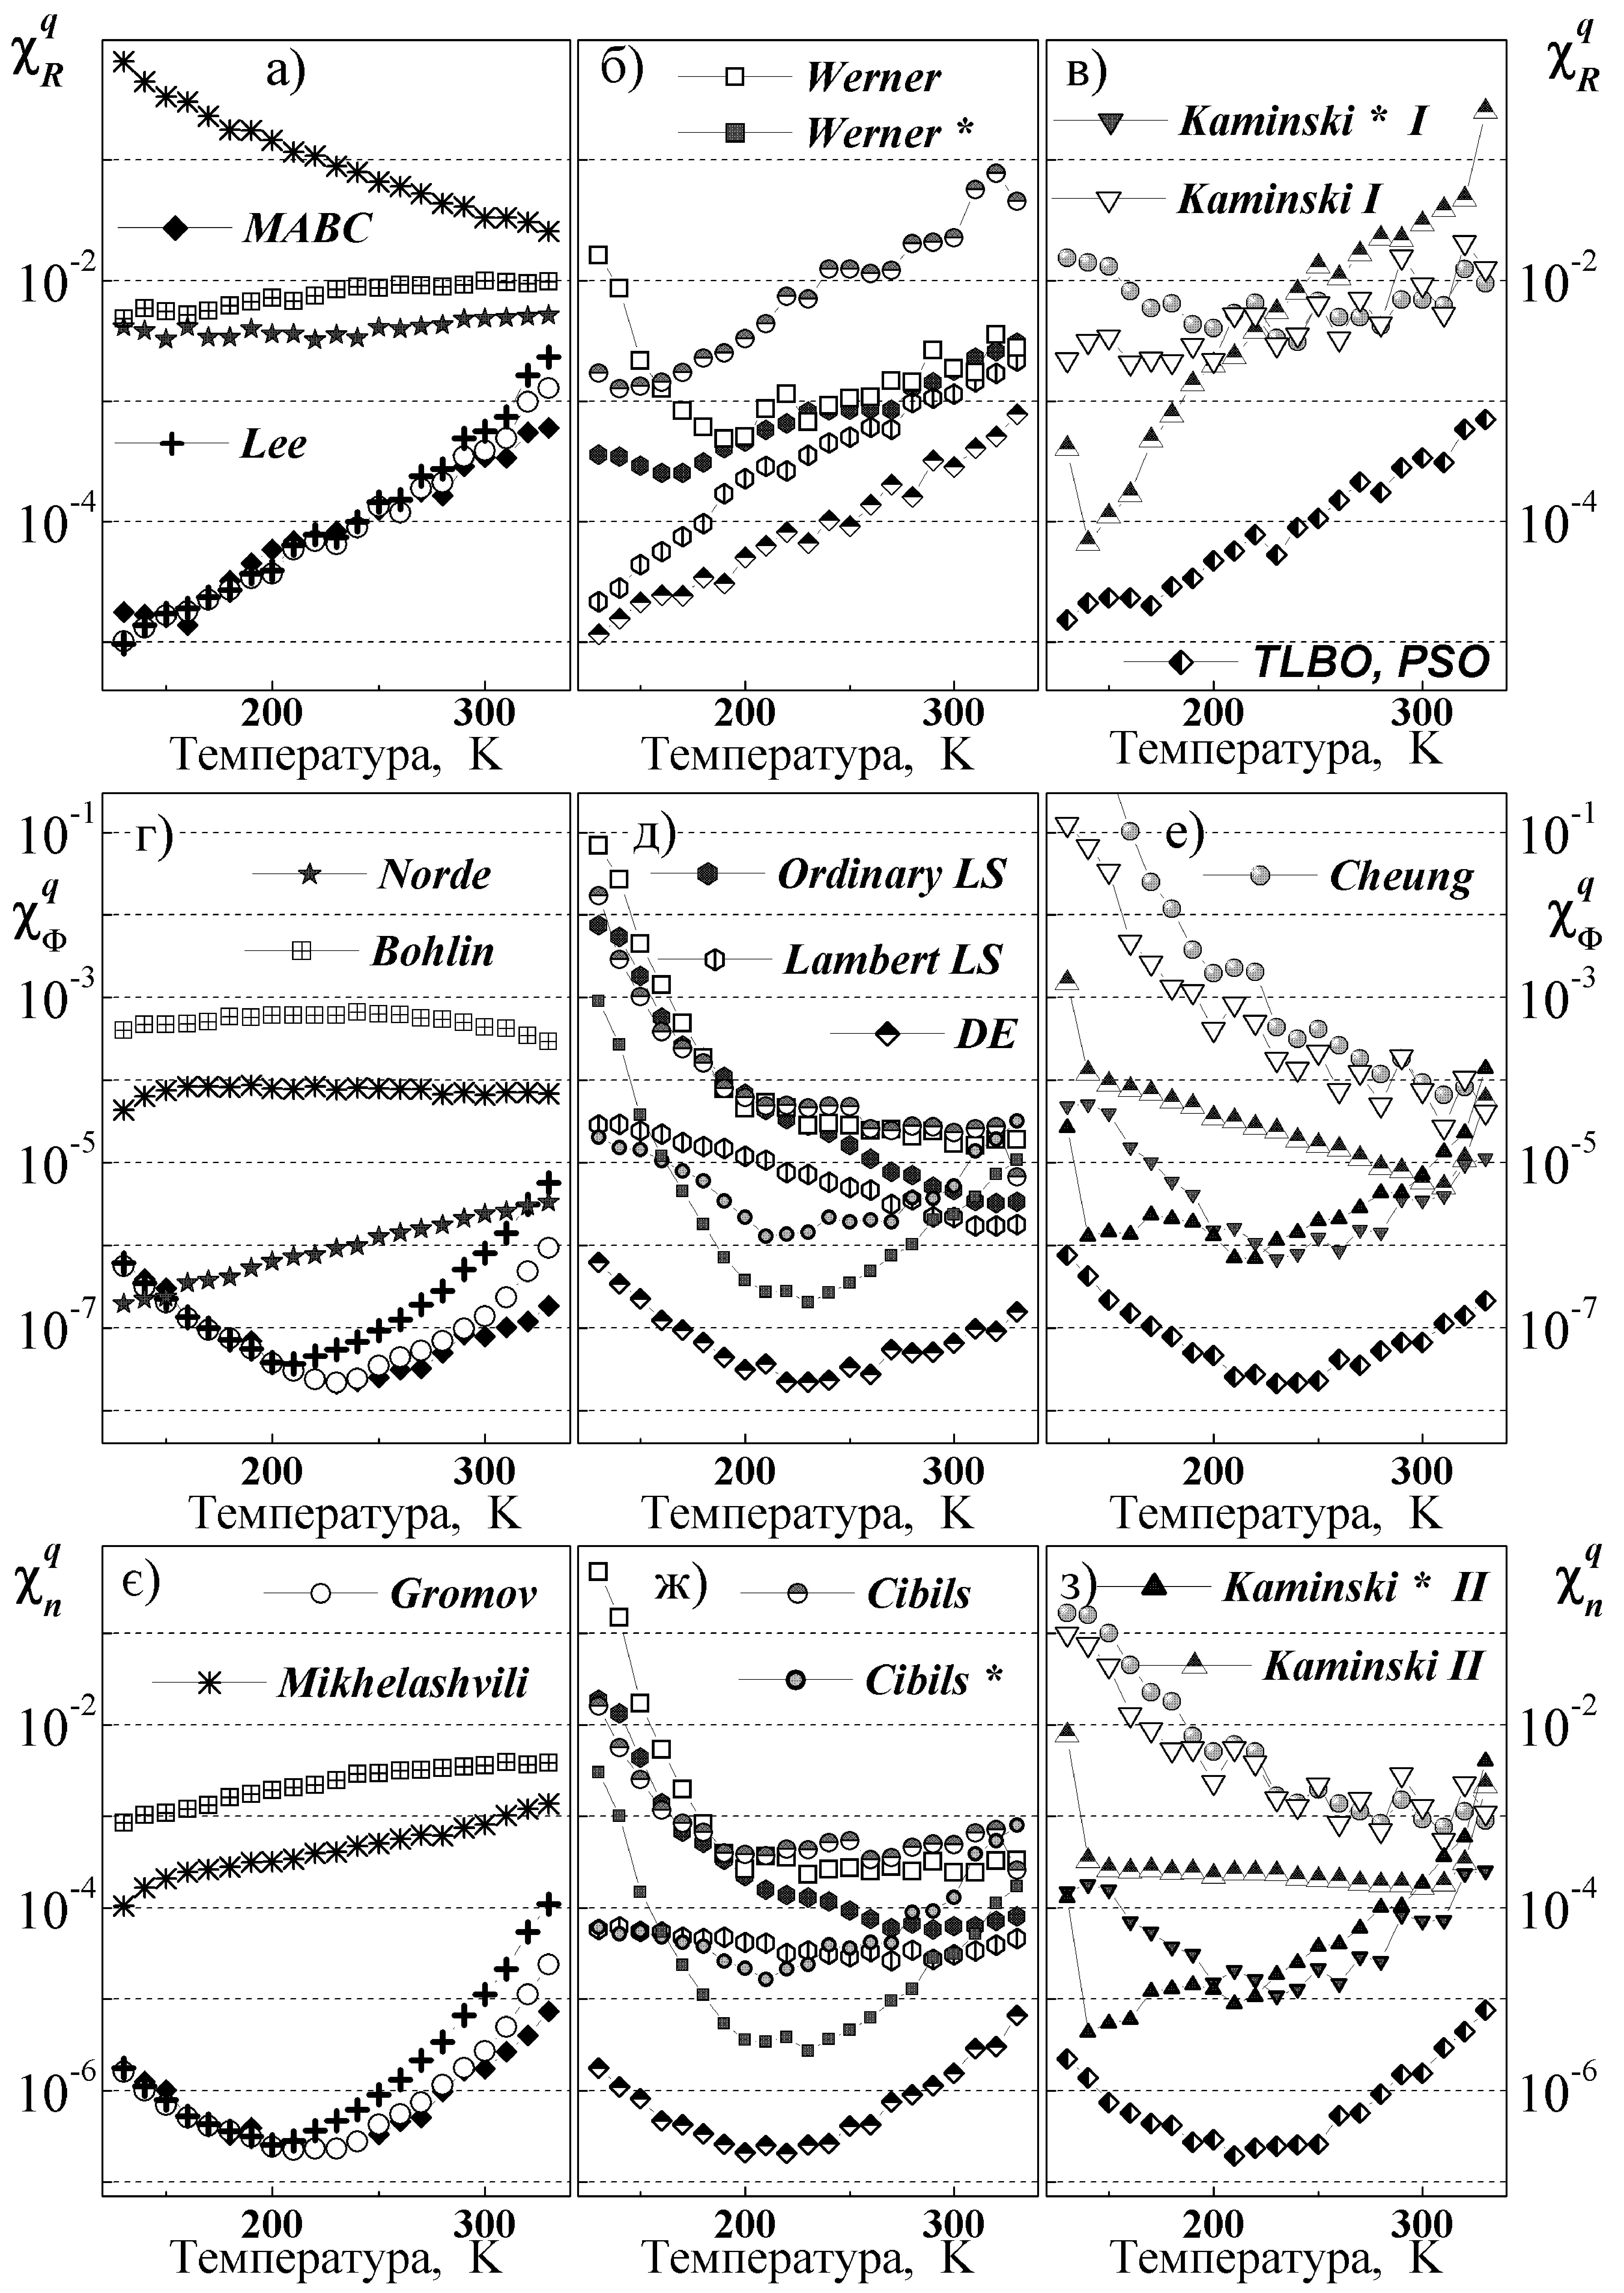
\includegraphics[width=0.9\textwidth]{figG1003}%
\caption{\label{figG1003}
Залежності точності визначення послідовного опору (а --- в), ВБШ (г --- е) та фактору неідеальності (є --- з) при використанні різних методів від температури.
Результати отримані при використанні наборів зашумлених даних.
$\sigma_V=0,3$~мВ, $\sigma_I^\varepsilon=1\%$.
}
\end{figure}

\begin{figure}
\center
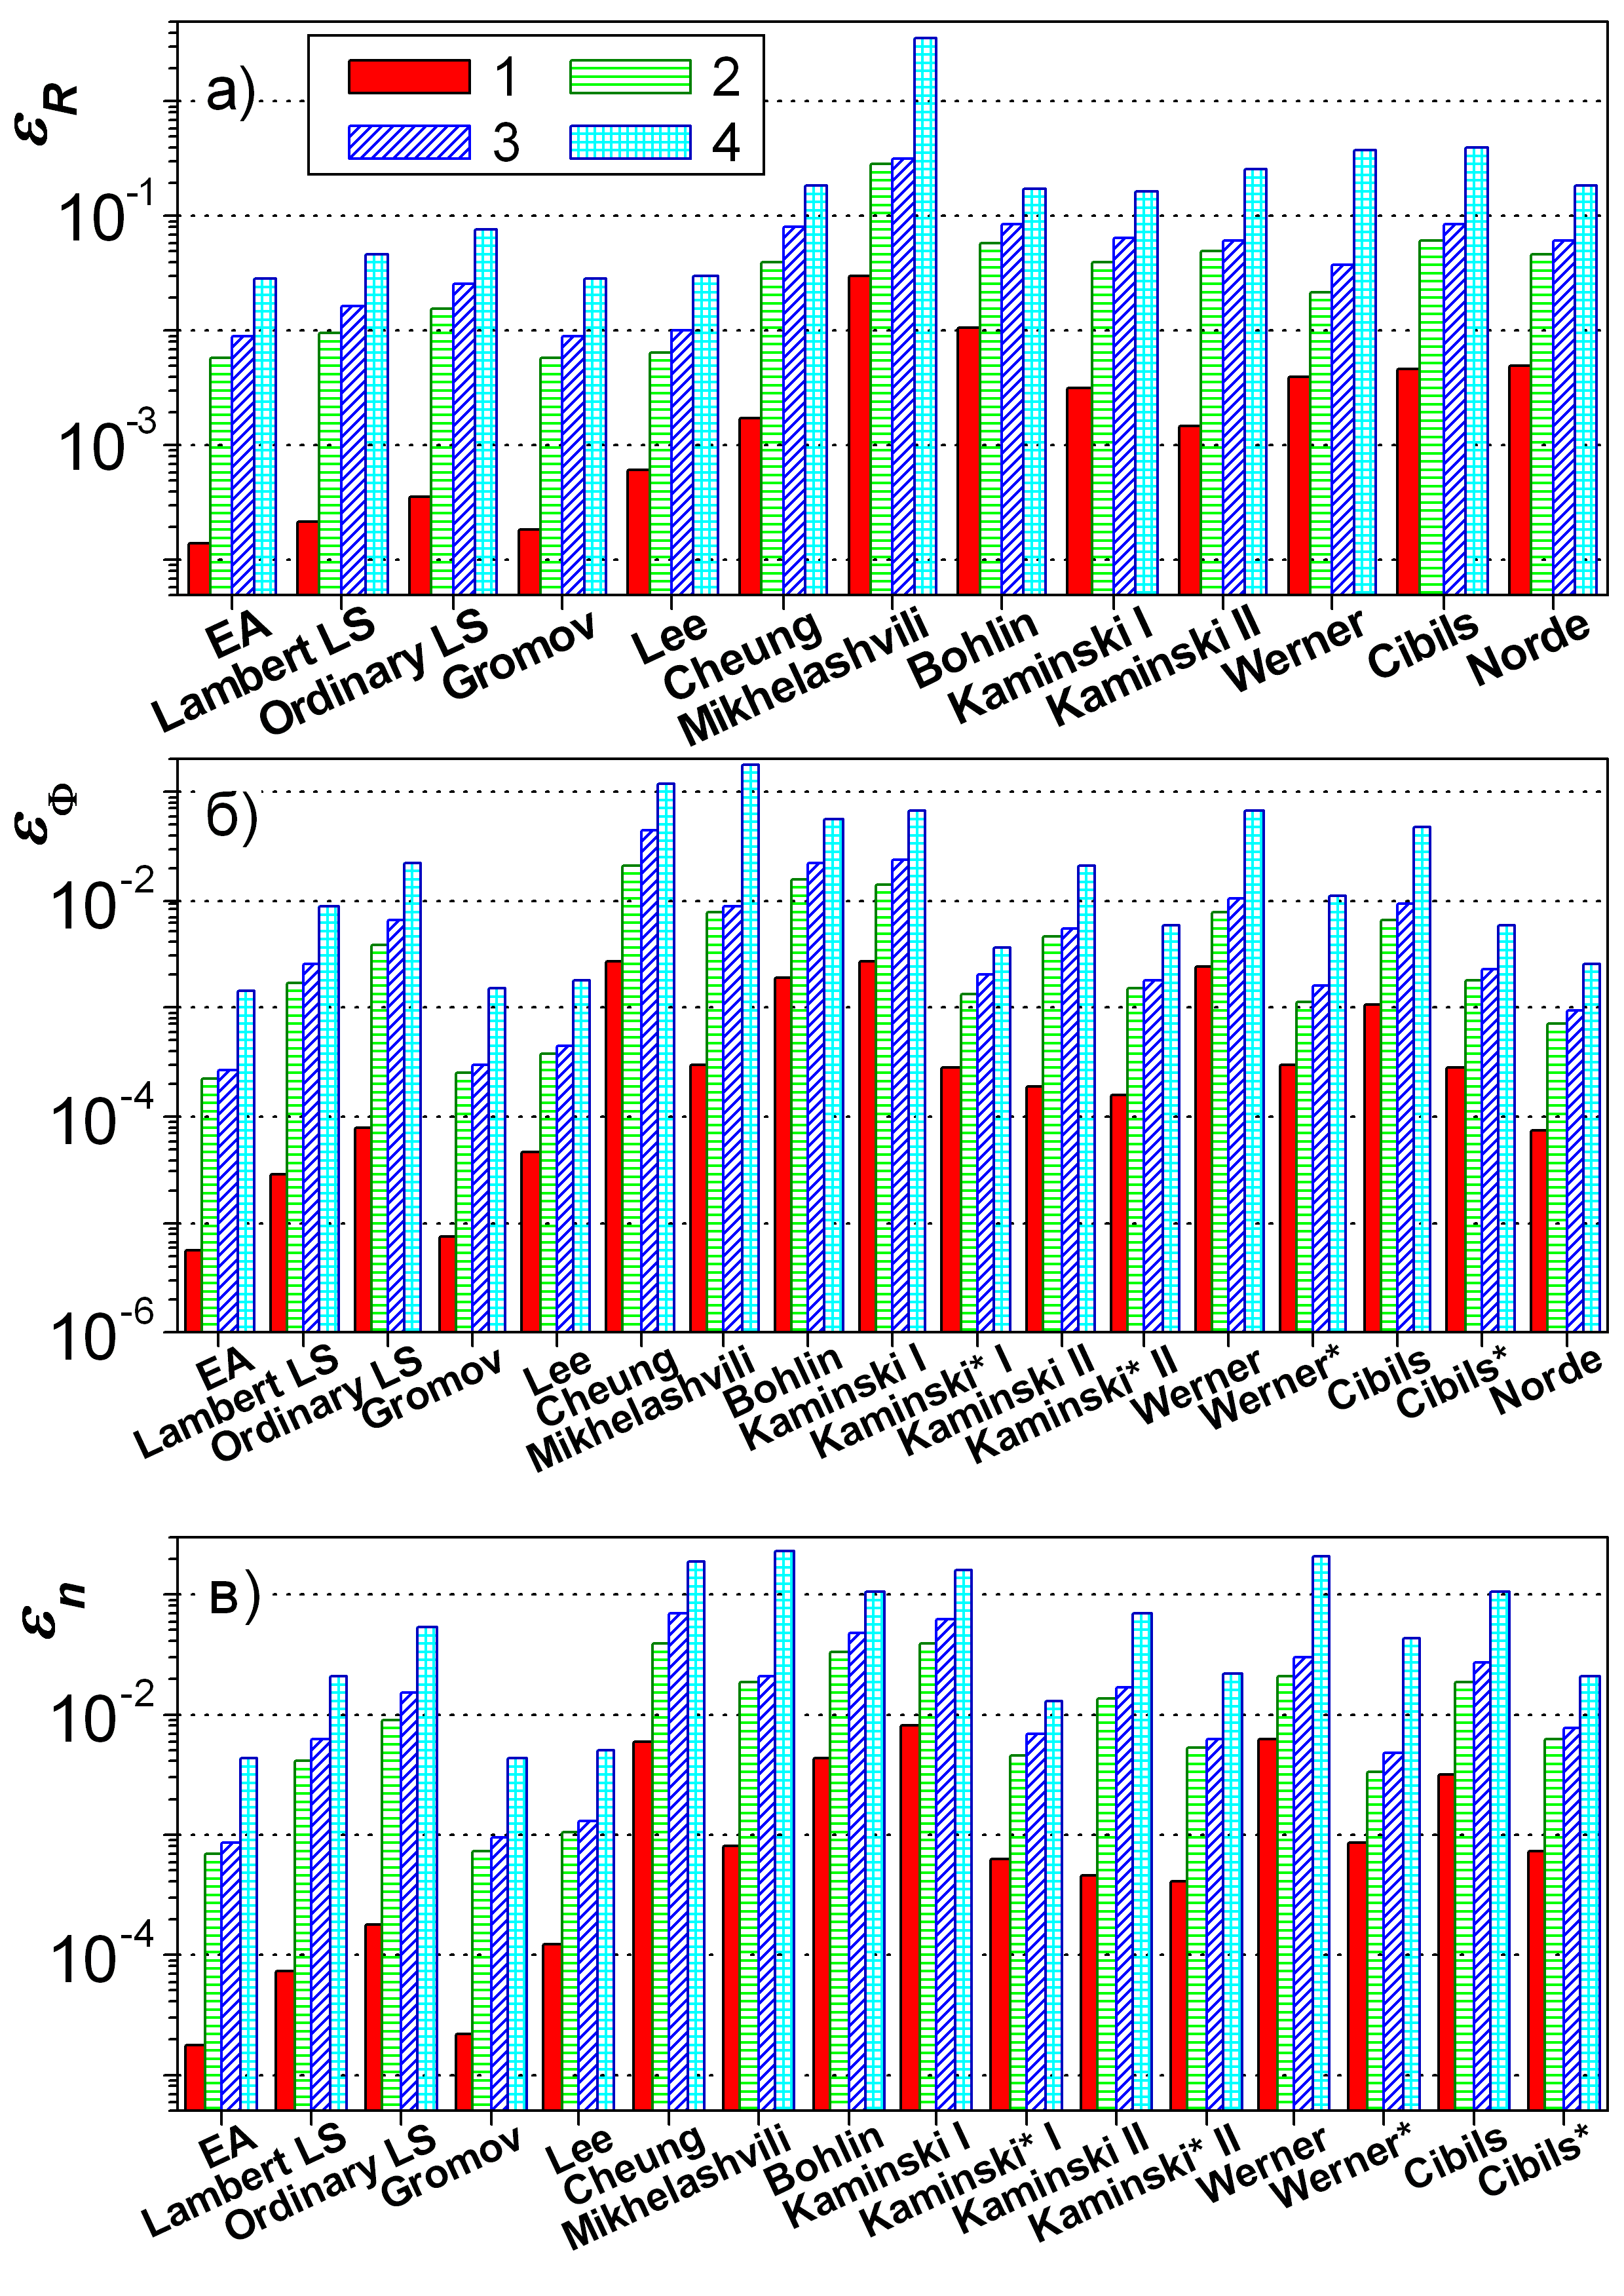
\includegraphics[width=0.9\textwidth]{figDiag}%
\caption{\label{figDiag}
Точність визначення $R_s$ (a), $\Phi_b$ (б) та $n_\mathrm{id}$ (в) з наборів зашумлених даних.
$\sigma_V$, мВ: 0 (1), 0,3 (2, 3), 2 (4).
$\sigma_I^\varepsilon$, \%: 0 (1), 0,5 (2), 1 (3, 4).
}
\end{figure}


У випадку, коли методи Werner, Cibils, Kaminskii~I або  Kaminskii~IІ застосовуються до зашумлених даних, визначення $n_\mathrm{id}$ шляхом апроксимації скорегованої ВАХ є більш точним, ніж ц випадку, коли ця величина визначається внаслідок апроксимації допоміжної функції.
Крім того, точність цих методів наближається до найкращих результатів інших методів і стає порівняною з точністю чисельних методів, або й навіть переважає її --- див. Рис.~\ref{figG1003}.
Метод Norde дозволяє достатньо точно визначати висоту бар'єру Шотки, проте фактор неідеальності можна отримати лише застосовуючи інші методи.

Залежності точності визначення параметрів від рівня шуму (від рівня випадкових помилок) показані ни Рис.~\ref{figErr}.
Наведені графіки отримані при використанні методу Gromov, проте вони є цілком типовими і для інших методів також.
Видно, що величини помилок при визначенні всіх параметрів практично лінійно залежать як від похибок вимірювання напруги, так і від відносних похибок сили струму.
Крім того, помилки визначення $\Phi_b$ та $n_\mathrm{id}$, викликані неточністю вимірювання напруги та сили струму, значно більші, ніж помилки визначення послідовного опору за тих самих умов.


\begin{figure}
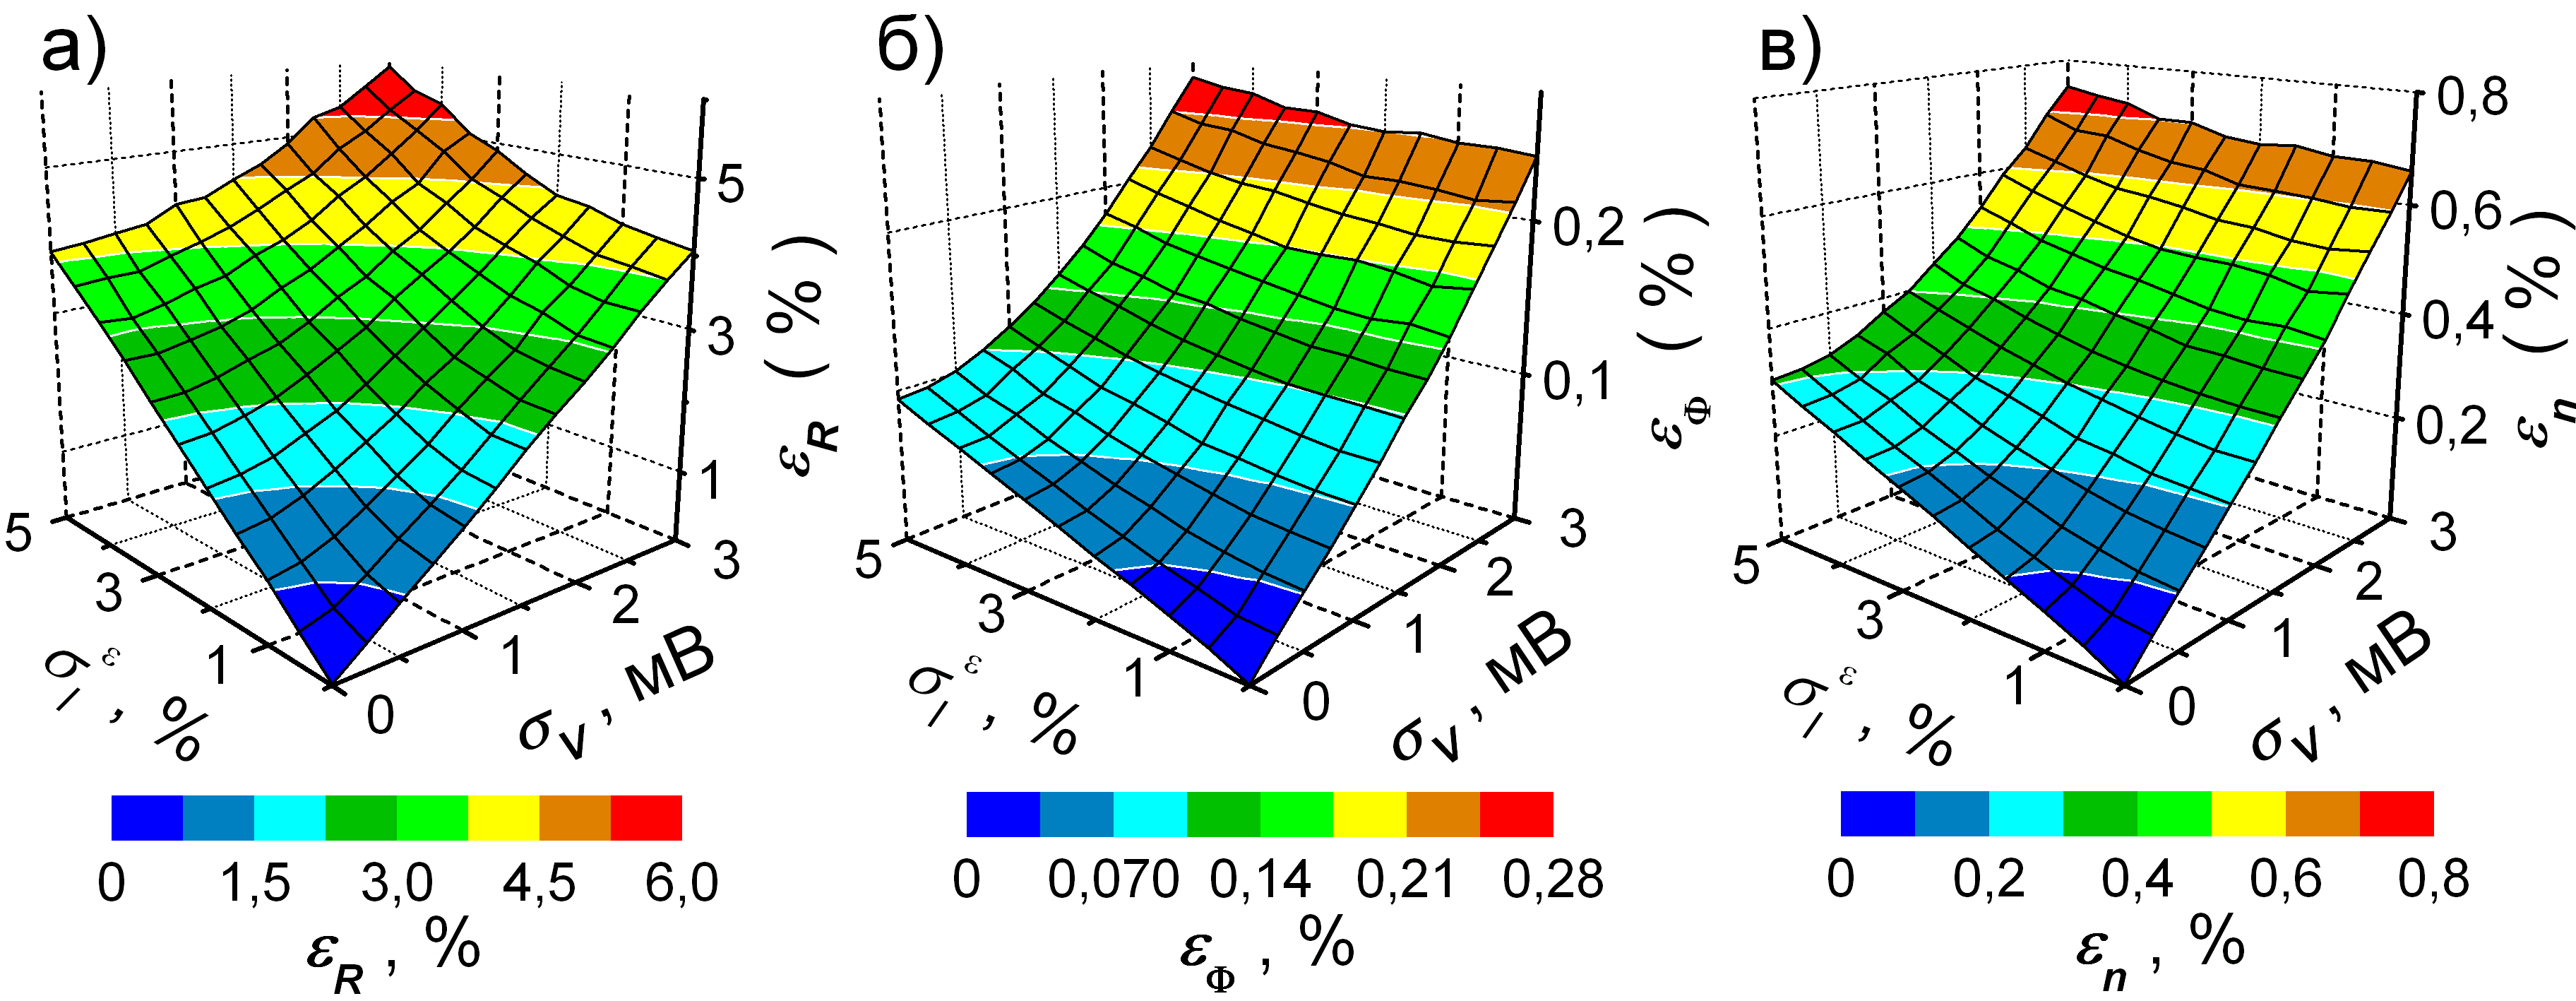
\includegraphics[width=1\textwidth]{figErr}%
\caption{\label{figErr}
Залежності точності визначення $R_s$ (a), $\Phi_b$ (б) та $n_\mathrm{id}$ (в) при використанні методу Gromov  від похибок вимірювання сили струму та напруги.
}
\end{figure}


\subsection{Визначення параметрів реальних структур МН}

Температурні залежності параметрів, отриманих з експериментальних ВАХ наведені на Рис.~\ref{figPract}.
Зауважимо, що в цьому випадку при застосуванні метода Bohlin були використані значення $\gamma_1=1,6$ та $\gamma_2=1,8$ замість  $\gamma_1=1,6$ та $\gamma_2=3,5$, для яких, як показано в розділі~\ref{AnMethod}, очікується менше значення похибки.
Це пов'язано з тим, що для діапазону сил струму, у якому були отримані експериментальні дані, відсутній мінімум функції Норда з $\gamma_N=3.5$.



\begin{figure}
\center
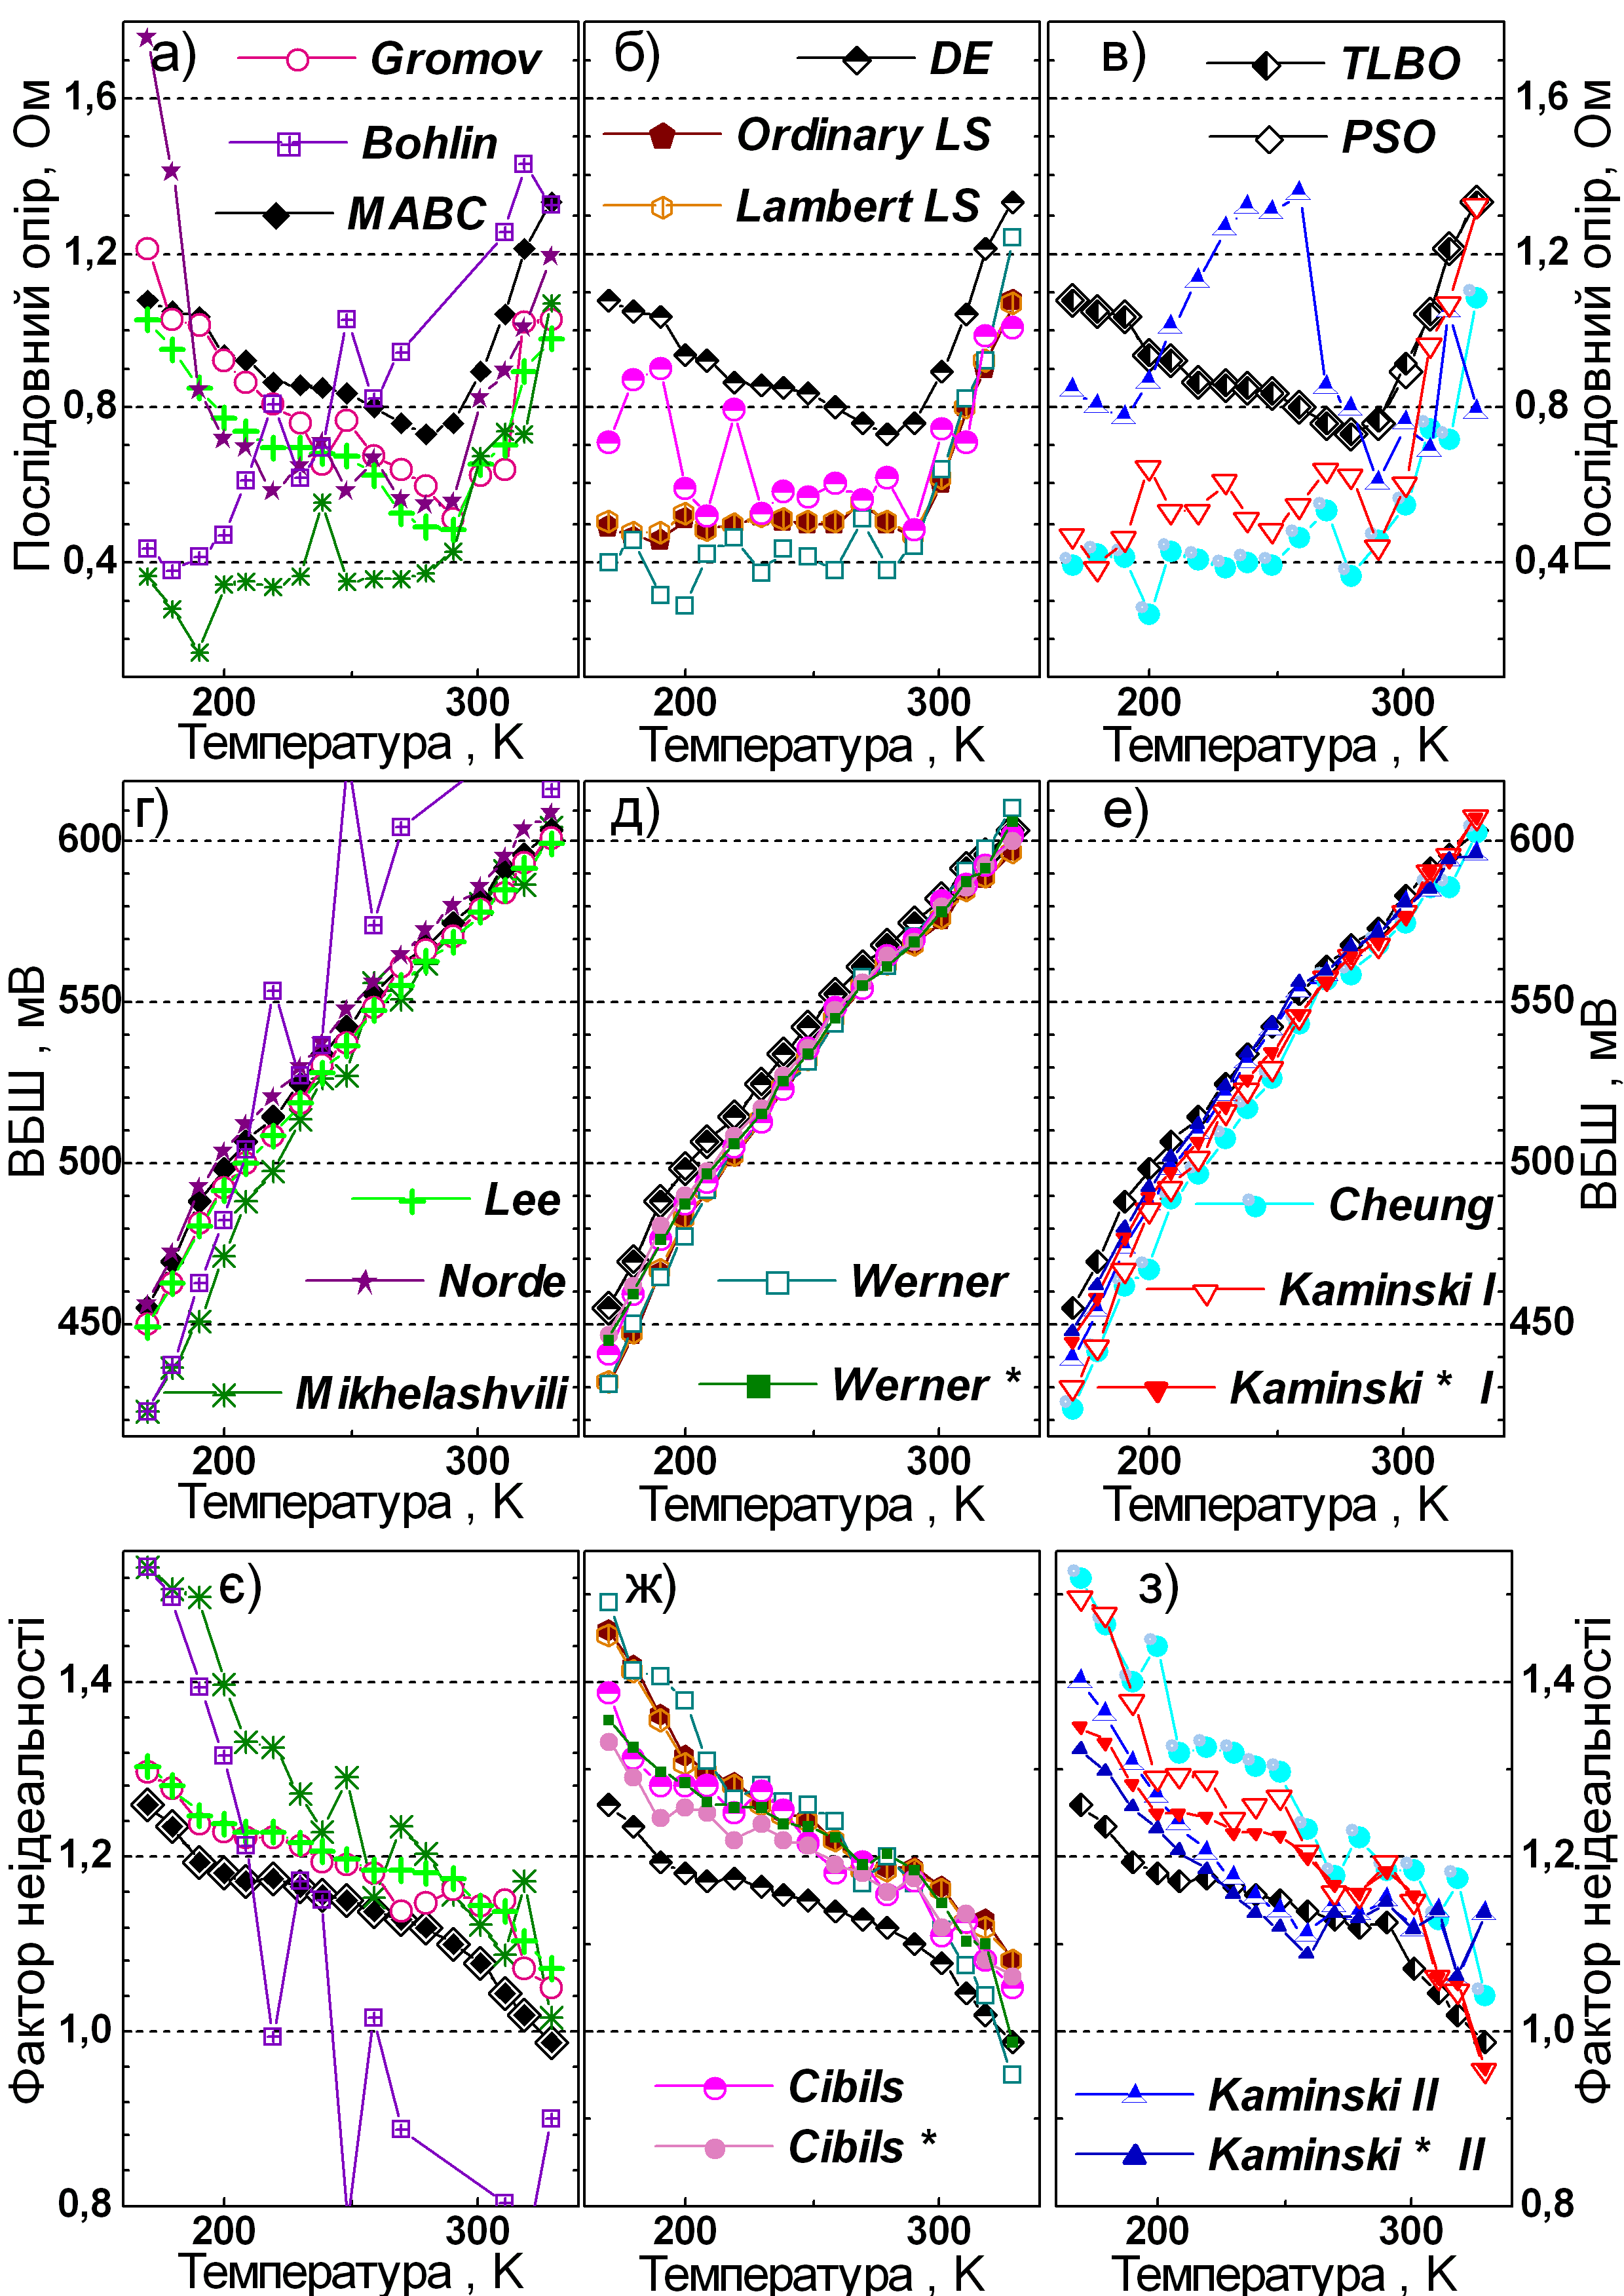
\includegraphics[width=0.9\textwidth]{figPract}%
\caption{\label{figPract}
Залежності точності визначення послідовного опору (а --- в), ВБШ (г --- е) та фактору неідеальності (є --- з) при використанні різних методів від температури.
Результати отримані при використанні експериментальних ВАХ.
}
\end{figure}

Виявлена температурна залежність висоти бар'єру, які відрізняється від виразу (\ref{eqFbT}), що використовувався при синтезі ВАХ, може бути пов'язана з неоднорідністю контакту МН \cite{Tung:MSE,Olikh:2013IEEE}.
Зростання послідовного опору при високих температурах в літературі \cite{Rs:Dokme} пов'язується з тим, що за цих умов визначальним для $R_s$ буде контактний опір, а не опір об'єму напівпровідника.

Зупинимось на отриманих температурних залежностях послідовного опору.
Використання ЕА, методів Gromov та Lee дозволяє виявити немонотонну температурну залежність $R_s$, причому абсолютні значення опору, отримані за допомогою різних методів, дещо відрізняються.
Взявши до уваги невелике значення послідовного опору (близько 1~Ом), а також виявлене раніше значне збільшення похибок методів Gromov та Lee при малих значеннях $R_s$ та великих $I_s$ (див. Рис.~\ref{figId},a, \ref{figR3D},a, \ref{figR3D},б та \ref{figG1003},a), можна зробити висновок, що величини, отримані при застосуванні еволюційних алгоритмів, більш правильні.
З фізичної точки зору, виявлена поступова зміна опору з температурою є цілком ймовірною.
При застосуванні числових методів отримана залежність $R_s$ від $T$ також є досить гладкою, проте її поведінка відрізняється від результатів ЕА при низьких температурах (див. Рис.~\ref{figPract},б).
З іншого боку, зашумленість температурних залежностей має свідчити про наявність помилок або під час вимірювань ВАХ, або під час визначення параметрів, а саме такі залежності виникають при застосуванні інших методів.

Подібні особливості характерні і для визначених залежностей ВБШ та фактора неідеальності.
Розкид значень $\Phi_b$ суттєво менший ніж для $n_\mathrm{id}$, що корелює з меншою величиною похибки визначення ВБШ (див. Рис.~\ref{figG1003} -- \ref{figErr}).
Найбільш погані результати отримані при використанні методів Bohlin, Mikhelashvili та Cheung.

Для оцінки розходжень виміряних та апроксимуючих ВАХ було використане середнє значення відхилення сили струму $\Delta_I$:
 \begin{equation}
 \label{eqMCur}
 \Delta_I=\frac{1}{N_p}\sum_{i=1}^{N_p}\left|\frac{I_{calc}(V_i)-I_i}{I_i}\right|.
 \end{equation}
При обчисленні $\Delta_I$, значення $I_{calc}(V_i)$ розраховувалися з використанням виразів (\ref{eqSDIV}--\ref{eqSDIs}) та параметрів, визначених при використанні різних методів.
Результати для трьох ВАХ, виміряних при різних температурах, наведені на Рис.~\ref{figPrAcc}.
Як видно, в цьому випадку еволюційні алгоритми, методи Gromov та Lee також продемонстрували свої переваги.


\begin{figure}
\center
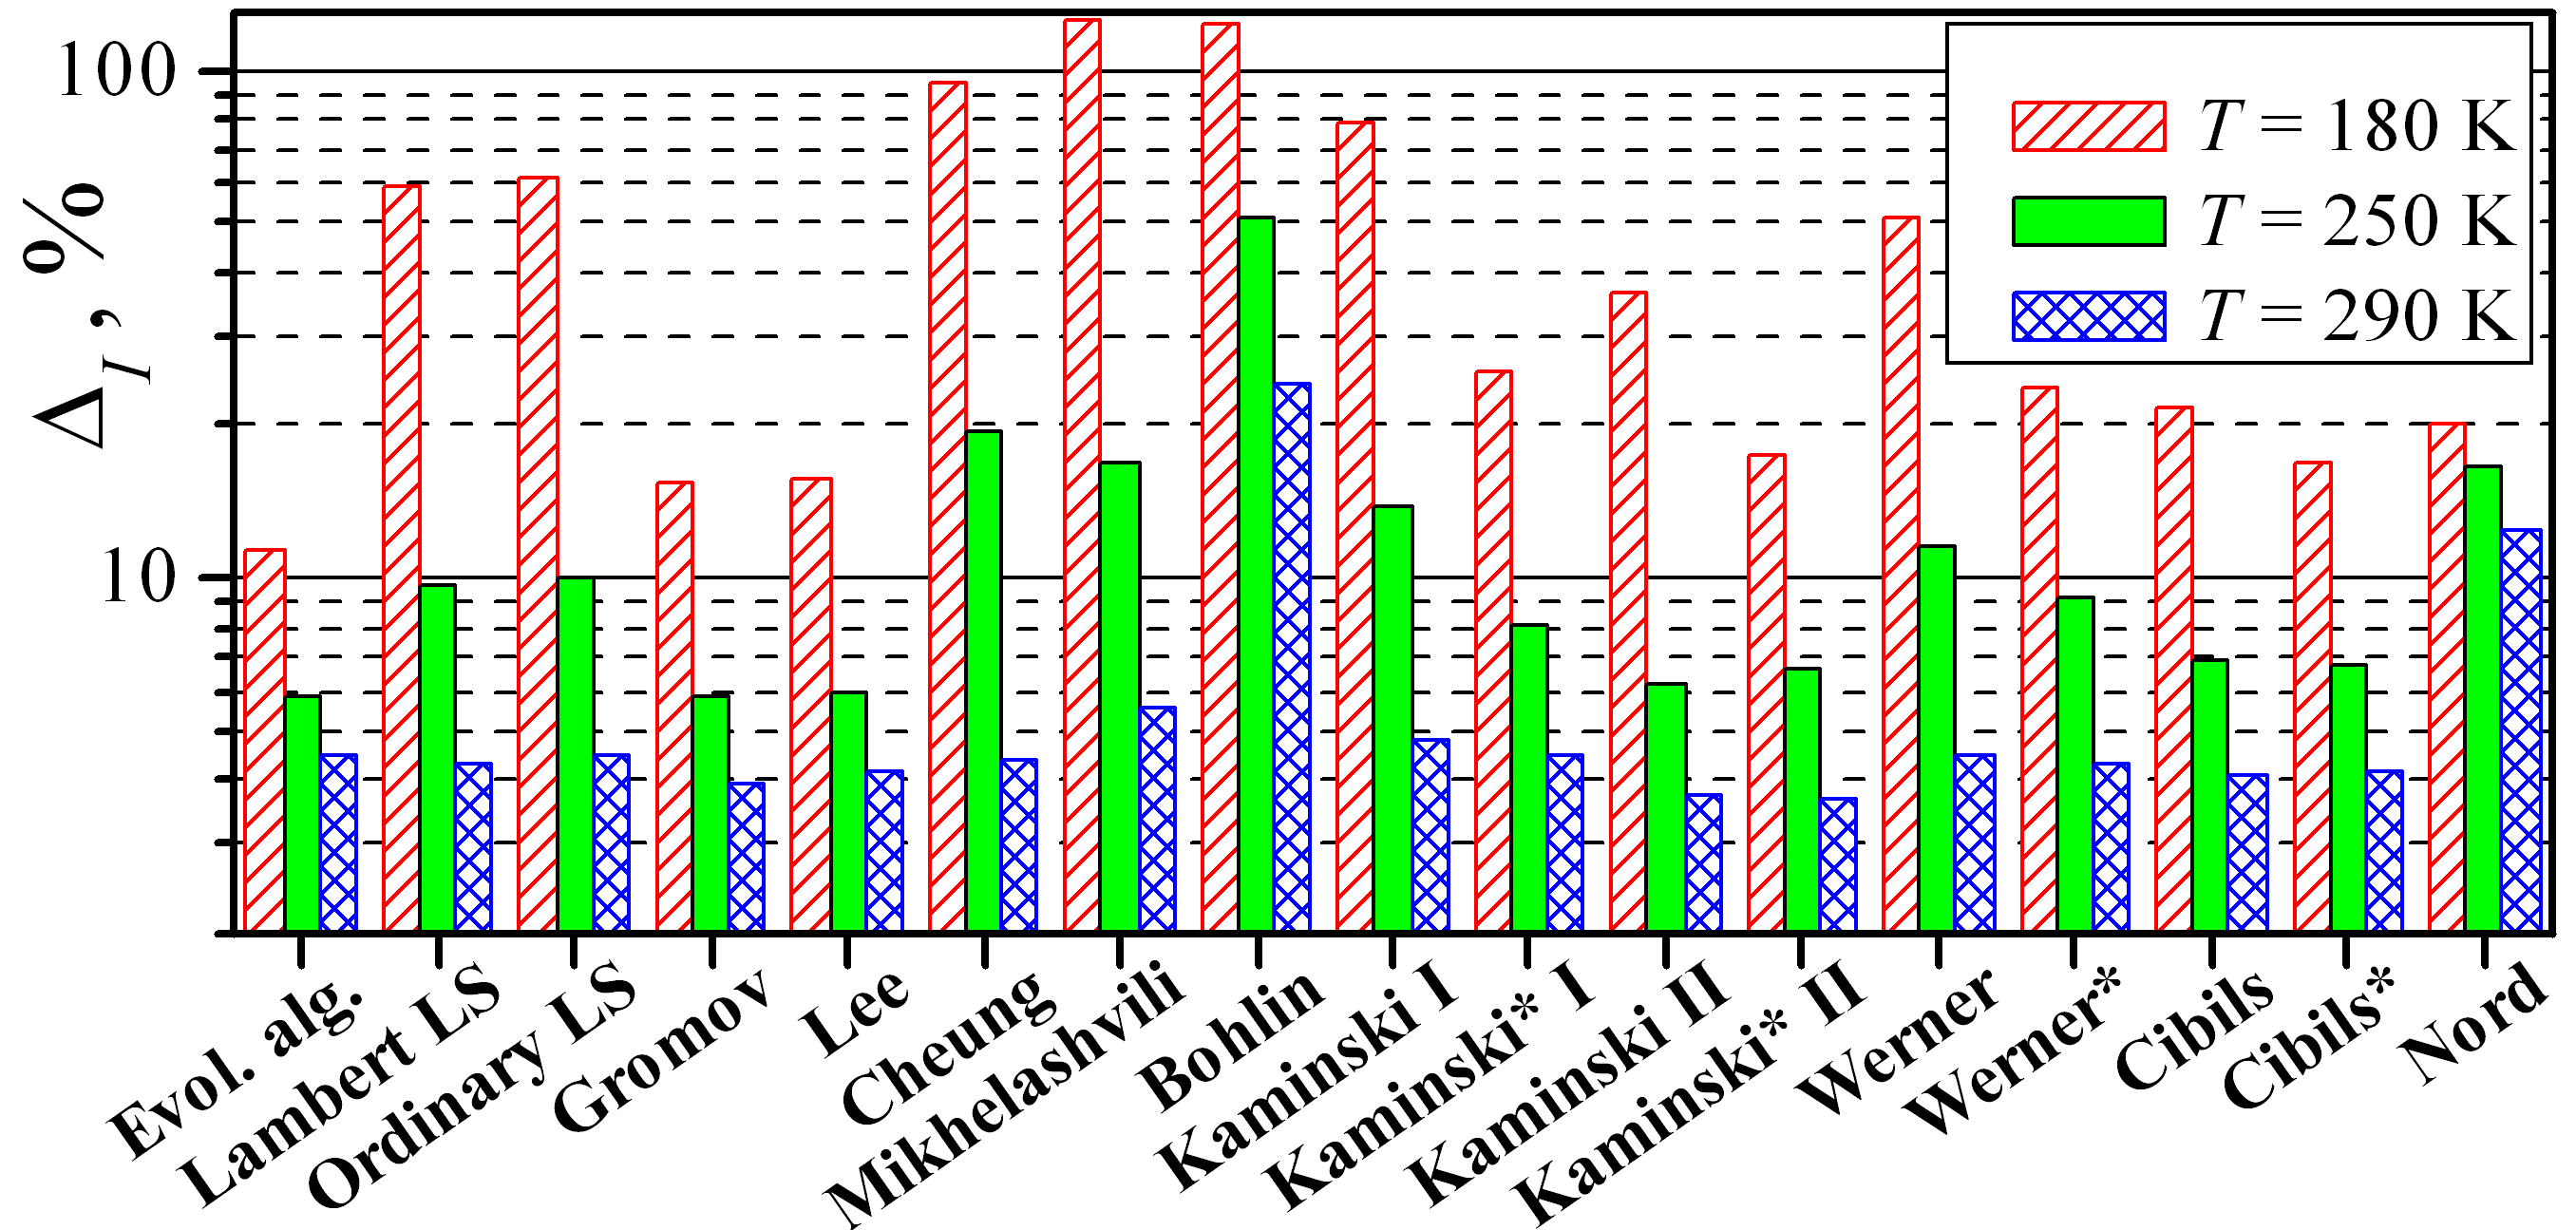
\includegraphics[width=1.0\textwidth]{figPrAcc}%
\caption{\label{figPrAcc}
Середні значення відносного відхилення розрахованих значень сили струму від експериментальних даних.
}
\end{figure}

Як було сказано раніше, і експериментальні ВАХ отримані для кремнієвих структур, і при синтезі даних вважалося, що ДШ створені з використанням саме цього напівпровідника. 
На мою думку, висновки щодо того, які методи є найбільш достовірними та такими, що мають перевагу, залишаються справедливими і при дослідженні структур не на основі кремнію.
Дійсно, для діодів з іншого матеріалу можуть спостерігатися зміни  величин $\Phi_b$, $n_\mathrm{id}$, $R_s$ та їх співвідношень.
Проте еволюційні алгоритми, методи Lee та Gromov з адаптивною процедурою довели свою перевагу для досить широкого діапазону значень параметрів.
З іншого боку, зміна матеріалу може викликати модифікацію
а)~температурної залежності точності визначення параметрів;
б)~абсолютного значення похибки.
Проте подібні зміни для конкретного напівпровідника можуть бути у першому наближені оцінені з використанням даних, наведених у Таблиці~\ref{tabIF}.

Проте необхідно підкреслити, що отримані результати будуть коректними для тих ДШ, для яких ВАХ описуються рівнянням~(\ref{eqSDIV}).
Так, наприклад, відхилення від цього закону характеристик реальних діодів може бути пов'язане з наявністю шунтуючого опору чи неоднорідністю бар'єру \cite{Tung:MSE,OlikhJAP}.
Проте в подібних випадках застосування еволюційних алгоритмів може суттєво спростити процедуру визначення параметрів структур МН.


\section*{Висновки до розділу \ref{Ch_MSMethod}}
\addcontentsline{toc}{section}{Висновки до розділу \ref{Ch_MSMethod}}	
  \begin{enumerate}
     \item Проведено тестування та порівняльне дослідження 16 методів визначення параметрів діодів Шотки з вольт--амперних характеристик.
           При цьому для аналізу були використані як експериментальні, так і синтезовані ВАХ.
     \item Проведено чисельний аналіз залежності величин похибок визначення ВБШ та послідовного опору в методі Норда від величини параметра $\gamma_N$ на масиві синтезованих ідеальних та зашумлених ВАХ.
     Виявлено, що похибка визначення висоти бар'ру зростає зі збільшенням параметру, тоді як залежність похибки оцінювання послідовного опору є немонотонною функцією $\gamma_N$.
     Показано, що найбільш оптимальним значенням є $\gamma_N=1,8$.
     \item Проведено чисельний аналіз залежності величин похибок визначення висоти бар'єру, фактору неідеальності та послідовного опору при використанні методу Бохліна від величин параметрів $\gamma_1$ та $\gamma_2$.
     Виявлено, що похибка екстрагування параметрів зростає при збільшенні величини $|\gamma_1-\gamma_2|$.
     Запропоновані оптимальні (для температурного діапазону $130\div330$~К) величини $\gamma_1=1,6$ та $\gamma_2=3,5$.
     \item Запропоновано адаптивну процедуру для вибору діапазону ВАХ, який використовується для побудови допоміжних функцій при застосуванні аналітичних методів визначення параметрів структур МН.
         Процедура базується на визначенні відхилення між апроксимуючою кривою та експериментальною.
         На прикладі аналітичного Gromov методу показано, що дана процедура дозволяє підвищити точність визначення параметрів, особливо у випадку низького рівня похибок вимірювання.
     \item Запропоновано модифікацію методу Mikhelashvili, яка дозволяє застосовувати його в автоматичному режимі до набору ВАХ.
     Вона полягає у послідовному використанні медіанного фільтру та процедури згладжування функції $\alpha(V)=d(\ln I)/d(\ln V)$ перед знаходженням положення її максимуму.
     Показано доцільність застосування запропонованої процедури для підвищення точності методу.
    \item Здійснена програмна реалізація еволюційних алгоритмів  диференційної еволюції, оптимізації зграї частинок,
модифікованої штучної бджолиної сім'ї і оптимізованого викладання та навчання при вирішенні задачі визначення параметрів структур МН.
Запропоновано та показано ефективність застосування цільової функції у вигляді суми квадратів відносних похибок апроксимації кожної з точок ВАХ.
Проведено визначення необхідної кількості поколінь для збіжності кожного з алгоритмів.
   \item Показано, що серед еволюційних алгоритмів MABC, DE, PSO та TLBO перший є найбільш придатним завдяки мінімальному часу роботи.
   \item Проаналізовано залежності точностей визначення послідовного опору, висоти бар'єру Шотки та фактора неідельності від величин параметрів та рівня випадкових помилок вимірювання ВАХ.
   \item Показано, що використання функції Ламберта при чисельному визначенні параметрів ДШ дозволяє зменшити похибки визначення та вплив на них інших факторів; з іншого боку, час роботи алгоритму зростає.    
   \item Показано, що серед всіх досліджених методів, найбільш придатними є еволюційні алгоритми (особливо MABC), метод Gromov з адаптивною процедурою та метод Lee.
    Перший є найбільш коректним при малих (декілька Ом)значеннях послідовного опору або великих значеннях струму насичення (високих температурах).     
  \end{enumerate}

Предсталені в даному розділі результати огляду, тестування та порівняльного аналізу методів визначення параметрів діодів Шотки будуть корисними для подальших дослідження та розробки
МН пристроїв.           % Глава 3
%\chapter*{\MakeUppercase{Висновки}}						% Заголовок
\addcontentsline{toc}{chapter}{\MakeUppercase{Висновки}}	% Добавляем его в оглавление

%% Согласно ГОСТ Р 7.0.11-2011:
%% 5.3.3 В заключении диссертации излагают итоги выполненного исследования, рекомендации, перспективы дальнейшей разработки темы.
%% 9.2.3 В заключении автореферата диссертации излагают итоги данного исследования, рекомендации и перспективы дальнейшей разработки темы.
%% Поэтому имеет смысл сделать эту часть общей и загрузить из одного файла в автореферат и в диссертацию:

%Основні результати представленої роботи полягають у наступному.
%% Согласно ГОСТ Р 7.0.11-2011:
%% 5.3.3 В заключении диссертации излагают итоги выполненного исследования, рекомендации, перспективы дальнейшей разработки темы.
%% 9.2.3 В заключении автореферата диссертации излагают итоги данного исследования, рекомендации и перспективы дальнейшей разработки темы.
\begin{enumerate}[leftmargin=0cm,itemindent=3em]
  \item Вперше експериментально досліджено вплив ультразвукового навантаження на параметри монокристалічних кремнієвих сонячних елементів у діапазоні температур $290\div340$~К
  та виявлена оборотна акустоіндукована деградація фотоелектричних властивостей, пов'язана зі зменшенням часу життя носіїв заряду в акустичному полі.
  Виявлено, що в умовах акустичного навантаження збільшується внесок у рекомбінаційні процеси більш мілких рівнів.
  Встановлено, що кисневмісні преципітати ефективно впливають на процеси рекомбінації та беруть участь у акусто--дефектній взаємодії.
  Запропоновано модель акустоактивного комплексного дефекту для пояснення особливостей акустоіндукованих ефектів.
 Виявлено ефект акустоіндукованого зменшення шунтуючого опору та запропоновано його пояснення із залученням моделі дислокаційно--індукованого імпедансу.

\item Вперше досліджено вплив ультразвукового навантаження на параметри кремнієвих структур з $p$-$n$ переходом, які були опромінені реакторними нейтронами та $\gamma$--квантами $^{60}$Co.
      Виявлено, що в опромінених структурах, порівняно з неопроміненими, спостерігається підвищення ефективності акустоіндукованого зменшення шунтуючого опору та часу життя неосновних носіїв заряду в базі діода.
      З'ясовано, що акустоіндуковані оборотні зміни фактора неідеальності та часу життя носіїв в області просторового заряду   мають різний знак в опромінених та неопромінених структурах.
      Встановлено, що нейтронно--опромінених діодах основними акустоактивними центрами є дивакансії,
      а в $\gamma$--опромінених --- комплекс вакансії та міжвузольного кисню
%      виявлені ефекти в нейтронно--опромінених діодах пов'язані зі впливом ультразвуку на стан дивакансій,  тоді як у гамма--опромінених діодах основним акустоактивним центром є комплекс вакансії та міжвузольного кисню.
     Виявлено, що комплекс з міжвузольного вуглецю та міжвузольного кисню практично не приймає участі в акусто--дефектній взаємодії.

\item  Проведено порівняльний аналіз та тестування 16 основних відомих методів визначення параметрів діодів Шотткі з вольт--амперних характеристик.
         Спираючись на результати тестування методів на експериментальних та синтезованих  ВАХ,
         запропоновано шляхи оптимізації методів Nord, Bohlin та Mikhelashvili з метою збільшення точності розрахунку.
      Запропоновано адаптивну процедуру для оптимізації вибору діапазону ВАХ, який використовується для побудови допоміжних функцій при застосуванні аналітичних методів визначення параметрів структур метал--напівпровідник.
       Показано, що така процедура дозволяє суттєво (приблизно на порядок при кімнатних температурах у випадку низького рівня похибок вимірювання) підвищити точність визначення параметрів.

   \item Встановлено, що найбільш ефективними методами з точки зору точності визначення параметрів та швидкості розрахунків є еволюційні алгоритми, метод Gromov з адаптивною процедурою та метод Lee.
    Показано, що використання функції Ламберта при чисельному визначенні параметрів діодів Шотткі дозволяє зменшити похибки.
    Визначено залежності точності визначення послідовного опору, висоти бар'єру Шотткі та фактора неідельності від величин параметрів та рівня випадкових помилок вимірювання вольт--амперних характеристик.

   \item
Встановлено, що при прямому зміщенні перенесення заряду в структурах Al$-n-n^+$--Si---Al з бар'єром Шотткі у діапазоні температур $130\div330$~К відбувається внаслідок термоелектронної емісії через неоднорідний контакт.
%Виконано експериментальне дослідження прямих і зворотних вольт--амперних характеристик структур Al$-n-n^+$--Si---Al з бар'єром Шотткі в діапазоні температур $130\div330$~К.
%Виявлено, що при підвищенні температури спостерігається збільшення висоти бар'єру та зменшення фактора неідеальності та встановлено механізм перенесення заряду із залученням моделі термоелектронної емісії через неоднорідний контакт у всьому діапазоні температур.
%       Показано, що отримані результати можна пояснити у рамках моделі термоелектронної емісії через неоднорідний контакт у всьому діапазоні температур.
        Показано, що при низьких температурах ($T<220$~К) суттєвим стає проходження заряду через області зі зниженим бар'єром і визначено середнє значення висоти бар'єру Шотткі в цих областях.
%          --- $54\pm4$~мВ.
     Виявлено, що при зворотному зміщенні в структурах Al---$n$--$n^+$--Si---Al перенесення заряду відбувається як внаслідок термоелектронної емісії через неоднорідний бар'єр, так і завдяки процесам тунелювання через глибокий центр (міжвузольний атом вуглецю).

\item
%Проведено експериментальне дослідження впливу $\gamma$--ви\-про\-мі\-ню\-ван\-ня $^{60}$Co на електрофізичні параметри структур Al$-n-n^+$--Si---Al.
     Показано, що опромінення $\gamma$-квантами $^{60}$Co структур Al$-n-n^+$--Si---Al суттєво підсилює процеси тунелювання носіїв заряду як при прямому зміщенні, так і при зворотному.
     Встановлено, що при прямому зміщенні тунельний механізм перенесення заряду стає основним в низькотемпературній області ($T<250$~К),
а при зворотному --- з'являється компонента струму, пов'язана з багатофононним тунелюванням.
 Виявлено, що висота бар'єру, фактор неідеальності та величина зворотного струму немонотонно змінюються при збільшенні поглинутої дози.
З'ясовано, що у випадку поглинутої дози $10^6$~рад зміна
електрофізичних
параметрів відбувається внаслідок накопичення дефектів акцепторного типу на границі метал--напівпровідник та укрупнення патчів, викликаного радіаційно підсиленим дислокаційним ковзанням.
При $10^7$~рад
визначальними механізмами змін властивостей діодів Шотткі є інтенсифікація процесів тунелювання внаслідок утворення значної кількості радіаційних дефектів та гетерування останніх в областях зі зниженим бар'єром.
Встановлено взаємозв'язок характеру дозової немонотонності зміни висоти бар'єру Шотткі та ступеню неоднорідності контакту.
%Показано, що характер дозової немонотонності зміни висоти бар'єру Шотки різний для   однорідних областей та для всього діоду загалом.


\item
Вперше досліджено вплив ультразвукового навантаження у динамічному режимі при кімнатній температурі на параметри кремнієвих діодів Шотткі Al$-n-n^+$--Si---Al.
Виявлено, що при поширенні акустичних хвиль спостерігаються оборотні зменшення висоти бар'єру,
збільшення зворотного струму та струму насичення, тоді як фактор неідеальності практично не змінюється.
З'ясовано, що ультразвукове навантаження практично не впливає на процеси прямого тунелювання та багатофононного тунелювання.
Встановлено, що вплив акустичного навантаження на термоемісійну складову струму структур пояснюється іонізацією дефектів на межі метал--напівпровідник
  внаслідок взаємодії ультразвуку з дислокаціями та радіаційними точковими порушеннями періодичності в неопромінених та опромінених структурах, відповідно.

\item
Вперше експериментально досліджено динамічний вплив ультразвукового навантаження в діапазоні частот $8\div28$~МГц на електричні властивості структур Mo/$n$--$n^{+}$--Si з бар'єром Шотткі в діапазоні температур $130\div330$~К.
 Виявлено акустоіндуковані оборотні зміни фактора неідеальності та висоти бар'єру Шотткі, причому зміни немонотонно залежать від температури і найбільш ефективний вплив ультразвуку спостерігається поблизу 200~K.
  Показано, що зі збільшенням частоти ультразвуку  спостерігається як загальне підвищення ефективності акустичного впливу на параметри кремнієвих діодів Шотткі,
так і зростання температури максимуму ефективності.
 Використовуючи модель неоднорідного контакту встановлено, що за умов ультразвукового навантаження відбувається збільшення висоти бар'єру як в області розташування патчів, так і за їх межами, а також уширюється розподіл параметрів патчів та збільшується їх ефективна густина.
З'ясовано, що механізм акустоіндукованих змін параметрів структур Mo/$n$--$n^{+}$--Si пов'язаний з рухом дислокаційних перегинів.
% Показано, що частотні та температурні особливості акустоіндукованих змін параметрів структур Mo/$n$--$n^{+}$--Si можуть бути пояснені в рамках
% моделі поглинання ультразвуку внаслідок руху дислокаційних перегинів.

\item Виявлено ефект оборотного збільшення зворотного струму структур Mo/$n$--$n^{+}$--Si за умов акустичного навантаження.
Встановлено, що ефект послаблюється при збільшенні температури та зміщення та посилюється при зростанні частоти ультразвуку.
Показано, що основними механізмами зворотного струму є термоелектронна емісія та тунелювання, стимульоване фононами;
в умовах поширення акустичних хвиль відбувається зменшення енергії активації рівнів, що беруть участь у тунелюванні,
густини заповнених інтерфейсних станів та коефіцієнта Пула--Френкеля.

\item Виявлено вплив мікрохвильового опромінення на параметри точкових дефектів у монокристалах $n$--6$H$--SiC, $n$--GaAs та епітаксійних структурах на основі арсеніду галію.
Встановлено, що причинами радіаційностимульованих змін поперечного перерізу захоплення електронів та розташування енергетичних рівнів пасток у забороненій зоні є
збільшення кількості міжвузольних атомів у приповерхневому шарі.
Показано, що викликані високочастотним опроміненням процеси перетворення дефектних комплексів інтенсифікуються за наявності механічних напруг.

\item Вперше експериментально досліджено вплив ультразвукової обробки на параметри структури Au--TiB$_x$--$n$--$n^+$--GaAs з контактом Шотткі
 залежно від частоти та потужності акустичної обробки.
 Встановлено, що при допороговій (менше 2,5~Вт/см$^2$) інтенсивності акустичної обробки відбувається збільшення однорідності параметрів арсенід галієвих діодів Шотткі, створених в єдиному технологічному процесі, пов'язане з
 акусто--стимульованою дифузією точкових дефектів.



\item Встановлено, що ультразвукова обробка викликає зменшення концентрації та звуження енергетичного спектра радіаційноіндукованих пасток  на інтерфейсі системи   Si--SiO$_2$.

%  На основе анализа \ldots
%  \item Численные исследования показали, что \ldots
%  \item Математическое моделирование показало \ldots
%  \item Для выполнения поставленных задач был создан \ldots
\end{enumerate}



Автор висловлює подяку
завідувачу кафедри загальної фізики Київського національного університету імені Тараса Шевченка,
проф.~Боровому~М.\:О. за всебічну підтримку досліджень та надану можливість наукового пошуку;
проф.~Конаковій~Р.\:В. (Інститут фізики напівпровідників ім. В.\:Є.~Лашкарьова НАНУ) за спрямування частини досліджень, надані зразки та позитивне ставлення до отриманих результатів;
%проф.~Оліху~Я.\:М. (Інститут фізики напівпровідників ім. В.\:Є.~Лашкарьова НАНУ) за можливість обговорення результатів та постійну технічну підтримку,
всім співавторам за можливість спільної роботи
та колективу кафедри загальної фізики
Київського національного університету імені Тараса Шевченка
за всебічну допомогу при проведенні експериментальних досліджень.

      % Заключение
%\chapter*{Перелік умовних скорочень та позначень}             % Заголовок
\addcontentsline{toc}{chapter}{Перелік умовних скорочень та позначень}  % Добавляем его в оглавление
\noindent
%\begin{longtabu} to \dimexpr \textwidth-5\tabcolsep {r X}
\begin{longtabu} to \textwidth {r X}
  CDLR& coupled defect level recombination,  рекомбінація у системі спарених рівнів дефектів\\
  DAT & defect--assisted tunneling, тунелювання за участю рівнів дефектів \\
  DE & differential evolution, метод диференційної еволюції \\
  FRC & fast--formed recombination center, швидко сформовані ВО дефекти \\
  NIEL & non--ionizing energy losses, втрати, не пов'язані з іонізацією \\
  MABC & modified artificial bee colony, метод  штучної бджолиної сім'ї\\
  OSFR & oxidization induced stacking--faults ring, кільцеві дефекти пакування, що виникли при окисненні \\
  PAT & phonon-assisted tunneling, стимулюване фононами тунелювання \\
  PSO & particle swarm optimization, метод оптимізації зграї частинок\\
  RT & running time, час, необхідний для визначення параметрів\\
  SCLC & space-charge limited current, струм, обмеженим просторовим зарядом \\
  SRC & slow--formed recombination center, повільно сформовані ВО дефекти\\
  TLBO & teaching learning based optimization, метод  оптимізованого викладання та навчання\\
  VRHC &thermally-assisted variable-range-hopping conduction, термічно--активована стрибкова провідність зі змінною довжиною стрибка \\
  AAД & акусто--активний дефект\\
  АДВ & акусто--дефектна взаємодія \\
  АІ & акусто--індукований\\
  АХ & акустична хвиля\\
  АЧХ & амплітудно--частотна характеристика\\
  ВАХ & вольт--амперна характеристика\\
  ВБШ & висота бар'єру Шотки\\
  ВТКС & високотемпературна компонента струму\\
  ВФХ & вольт--фарадна характеристика\\
  ГР &глибокий рівень \\
  ДШ & діод Шотки\\
  ЕА & еволюційний алгоритм\\
  КНО &  квазі--нейтральна область \\
  КП & кисневмісні преципітати\\
  КСЕ & кремнієвий сонячний елемент\\
  MH & метал--напівпровідник \\
  МХО & мікро--хвильова обробка\\
  НТКС & низькотемпературна компонента струму\\
  ОПЗ & область просторового заряду \\
  ПАН & поперечна акустоелектрична напруга\\
  ПЕ & польова емісія\\
  ППЗ & поперечний переріз захоплення \\
  РД & радіаційний дефект \\
  ТД &точковий дефект \\
  ТЕ & термоелектронна емісія \\
  ТПЕ & термопольова емісія \\
  УЗ & ультразвук \\
  УЗН & ультразвукове навантаження \\
  УЗО & ультразвукова обробка \\
  ШРХ & теорія Шоклі--Ріда--Хола  \\
$\alpha$ & коефіцієнт поглинання світла  \\
$\alpha_R$ & температурний коефіцієнт опору\\
$\alpha_\mathrm{\,FB}$ & температурний коефіцієнт ВБШ в наближені плоских зон\\
$\beta$ & коефіцієнт квантового виходу  \\
$\beta_1$, $\beta_2$  & коефіцієнти Варшні  \\
$\Delta P$ & абсолютна АІ зміна параметра $P$\\
$\varepsilon$ & діелектрична проникність матеріалу  \\
$\varepsilon_0$ & діелектрична стала \\
$\varepsilon_P$ & відносна AI зміна параметра $P$\\
$\xi_\mathtt{cur}$ & відносна деформація приповерхневих кристалічних площин\\
$\xi_\mathtt{US}$& амплітуда деформації ґратки при поширенні УЗ\\
$\vartheta$ & темп генерації РД\\
$\lambda$ &довжина хвилі падаючого світла\\
$\rho_\mathtt{LNO}$ & густина ніобату літію\\
$\rho_\mathtt{Si}$ & густина кремнію\\
$\sigma_\Phi0$ & стандартне відхилення висоти бар'єру при нульовому зміщенні\\
$\sigma_n$& поперечний переріз захоплення електронів дефектом\\
$\sigma_p$& поперечний переріз захоплення дірок дефектом\\
$\tau$ & час релаксації заряду на пастках\\
$\tau_{g}$ &ефективний час життя носіїв заряду в ОПЗ\\
$\tau_{n}$ &ефективний час життя електронів\\
$\tau_{n,\mathtt{RD}}$ & час життя електронів при рекомбінації на РД\\
$\upsilon_\mathtt{LNO}$ & швидкість звуку в ніобаті літію\\
$\upsilon_{\mathrm{th},n}$ & теплова швидкість електронів\\
$\upsilon_{\mathrm{th},p}$ & теплова швидкість дірок\\
$\upsilon_\mathtt{Si}$ & швидкість звуку в кремнії\\
$\Phi_b$ & ВБШ при нульовому зміщенні\\
$\Phi_{b}^0$ & середнє значення ВБШ при нульовому зміщенні (ВБШ в однорідній області) \\
$\Phi_{b}^\mathrm{FB}$ & ВБШ в наближені плоских зон \\
$\Psi$ & флюєнс опромінення\\
$\phi_0$ & рівень нейтральності інтерфейсних станів у структурі МН\\
$\zeta$ & диференційний показник нахилу ВАХ \\
$\omega_{ph}$ & частота фонону\\
$\omega_\mathtt{US}$ & циклічна частота АХ\\
$A$ & площа зразка \\
$A_\mathtt{LNO}$ & площа п'єзоперетворювача\\
$A^*$ & ефективна стала Річардсона \\
$a$ & стала ґратки \\
$a_B$ & радіус Бора\\
$B$ & коефіцієнт динамічної в'язкості \\
$b$ & модуль вектора Бюргерса \\
$C$ & ємність діоду Шотки\\
$c$ & швидкість світла\\
$D$ & доза опромінення\\
$D_d$ & displacement damage dose, ефективна доза, пов'язана з дефектоутворенням\\
$D_{ss}$ & густина інтерфейсних станів у структурі МН\\
$E_g$ & ширина забороненої зони\\
$E_i$ & положення рівня Фермі у власному напівпровіднику\\
$E_t$ & положення енергетичного рівня, зв'язаного з дефектом\\
$F\!F$ & фактор форми КСЕ\\
$F_m$ & напруженість електричного поля на границі розділу метал-напівпровідник \\
$f_r$& резонансна частота п'єзоперетворювача\\
$f_\mathtt{US}$& частота УЗ\\
$G$ & модуль зсуву \\
$h$, $\hbar$ & стала Планка\\
$I$ & струм\\
$I_s$ & струм насичення\\
$I_R$ & зворотний струм\\
$J$ & густина струму\\
$J_{ph}$ & густина фотогенерованого струму\\
$J_{sс}$ & густина струму короткого замикання\\
$k$ & стала Больцмана\\
$L_n$ & довжина дифузії електронів\\
$m*$ &  ефективна маса електрону \\
$N_c$ & ефективна густина станів біля дна зони провідності\\
$N_d$ & концентрація електронів поблизу контакту МН\\
$N_{t,\mathtt{RD}}$ & концентрація радіаційних дефектів\\
$N_v$ & ефективна густина станів біля вершини валентної зони\\
$n_i$ & концентрація власних носіїв заряду\\
$n$ & концентрація електронів\\
$n_\mathrm{id}$ & фактор неідеальності\\
$n_n$ & концентрація основних носіїв у електронному напівпровіднику \\
$n_p$ & концентрація неосновних носіїв у дірковому напівпровіднику \\
$q$ & елементарний заряд\\
$p$ & концентрація дірок \\
$p_n$ & концентрація неосновних носіїв у електронному напівпровіднику \\
$p_p$ & концентрація основних носіїв у дірковому напівпровіднику \\
$R$ & темп рекомбінації \\
$R_\mathtt{cur}$ & радіус кривизни зразка \\
$R_{\mathtt{DA}}$ & параметр зв'язку у моделі CDLR\\
$R_{ph}$ & коефіцієнт відбивання світла\\
$R_s$ & послідовний опір\\
$R_{sh}$ & шунтуючий опір\\
$T$ & абсолютна температура\\
$T_0$ & константа температурної залежності фактора неідеальності\\
$T_\mathtt{US}$ & період АХ\\
$t$ & час\\
$t_\mathtt{MWT}$ & час експозиції при МХО\\
$u_\mathtt{US}$&амплітуда зміщень атомів при поширенні УЗ\\
$V$ & напруга\\
$V_{bb}$ & вигин зон напівпровідника поблизу контакту\\
$V_d$ & падіння напруги в околі бар'ру\\
$V_n$ & різниця потенціалів між дном зони провідності та положенням рівня Фермі в об'ємі напівпровідника\\
$V_{oc}$ & напруга холостого ходу\\
$V_R$ & зворотна напруга\\
$V_\mathtt{TAV}$ & величина ПАН\\
$V_\mathtt{RF}$ & амплітуда високочастотної напруги, прикладеної до п'єзоперетворювача\\
$V_v$ & об'єм кристалу\\
$W_{ph}$ & інтенсивність освітлення \\
$W_\mathtt{US}$ & інтенсивність акустичної хвилі\\

\end{longtabu}
\addtocounter{table}{-1}% Нужно откатить на единицу счетчик номеров таблиц, так как предыдующая таблица сделана для удобства представления информации по ГОСТ





        % Список сокращений и условных обозначений
%\chapter*{Словарь терминов}             % Заголовок
\addcontentsline{toc}{chapter}{Словарь терминов}  % Добавляем его в оглавление

\textbf{TeX} "--- Cистема компьютерной вёрстки, разработанная американским профессором информатики Дональдом Кнутом

\textbf{Панграмма} "--- Короткий текст, использующий все или почти все буквы алфавита
      % Словарь терминов
%\clearpage                                  % В том числе гарантирует, что список литературы в оглавлении будет с правильным номером страницы
%\hypersetup{ urlcolor=black }               % Ссылки делаем чёрными
%\providecommand*{\BibDash}{}                % В стилях ugost2008 отключаем использование тире как разделителя
%\urlstyle{rm}                               % ссылки URL обычным шрифтом
\ifdefmacro{\microtypesetup}{\microtypesetup{protrusion=false}}{} % не рекомендуется применять пакет микротипографики к автоматически генерируемому списку литературы
\insertbibliofull                           % Подключаем Bib-базы
\ifdefmacro{\microtypesetup}{\microtypesetup{protrusion=true}}{}
%\urlstyle{tt}                               % возвращаем установки шрифта ссылок URL
%\hypersetup{ urlcolor={urlcolor} }          % Восстанавливаем цвет ссылок
      % Список литературы
%\clearpage
\ifdefmacro{\microtypesetup}{\microtypesetup{protrusion=false}}{} % не рекомендуется применять пакет микротипографики к автоматически генерируемым спискам
\listoffigures  % Список изображений

%%% Список таблиц %%%
% (ГОСТ Р 7.0.11-2011, 5.3.10)
\clearpage
\listoftables   % Список таблиц
\ifdefmacro{\microtypesetup}{\microtypesetup{protrusion=true}}{}
\newpage           % Списки таблиц и изображений (иллюстративный материал)
%%\appendix
%%% Оформление заголовков приложений ближе к ГОСТ:
\setlength{\midchapskip}{20pt}
\renewcommand*{\afterchapternum}{\par\nobreak\vskip \midchapskip}
\renewcommand\thechapter{\Asbuk{chapter}} % Чтобы приложения русскими буквами нумеровались
   % Предварительные настройки для правильного подключения Приложений
%\chapter{\MakeUppercase{список публікацій за темою дисертації}} \label{AppendixA}
\chapter*{\MakeUppercase{Додатки}}						% Заголовок
\addcontentsline{toc}{chapter}{\MakeUppercase{Додатки}}
\section*{Додаток А. Список публікацій за темою дисертації та відомості про апробацію результатів}


\begin{center}%
\emph{Наукові праці, в яких опубліковано основні наукові результати дисертації}
\end{center}%
%\subsection*{Наукові праці, в яких опубліковано основні наукові результати дисертації}
\begin{enumerate}[label=\arabic*.,leftmargin=1em,itemindent=1em]
%\begin{enumerate}[label=\arabic*.,leftmargin=0em,itemindent=2em]
%\setcounter{enumi}{25}
\item
Acousto--defect interaction in irradiated and non--irradiated silicon
  $n^+$--$p$ structure~/ O.~Ya.~Olikh, A.~M.~Gorb, R.~G.~Chupryna,
  O.~V.~Pristay-Fenenkov~// \emph{J. Appl. Phys.} --- 2018. --- Apr. ---
 Vol. 123, no.~16. --- P.~161573--1--161573--12.

\item
\emph{Olikh,~O.Ya.} Acoustically driven degradation in single crystalline
  silicon solar cell~/ O.Ya.~Olikh~// \emph{Superlattices Microstruct.} ---
  2018. --- May. ---
  Vol. 117. ---
  P.~173--188.

\item
\emph{Olikh,~Oleg}. On the mechanism of ultrasonic loading effect in
  silicon--based {S}chottky diodes~/ Oleg~Olikh, Katerina~Voytenko~//
  \emph{Ultrasonics}. ---
  2016. --- Mar. ---
  Vol.~66, no.~1. ---
  P.~1--3.

\item
Effect of ultrasound on reverse leakage current of silicon {S}chottky barrier
  structure~/ O.~Ya.~Olikh, K.~V.~Voytenko, R.~M.~Burbelo, Ja.~M.~Olikh~//
  \emph{Journal of Semiconductors}. ---
  2016. --- Dec. ---
  Vol.~37, no.~12. ---
  P.~122002--1--122002--7.

\item
\emph{Olikh,~O.~Ya.} Review and test of methods for determination of the
  {S}chottky diode parameters~/ O.~Ya.~Olikh~// \emph{J. Appl. Phys.} ---
  2015. --- Jul. ---
  Vol. 118, no.~2. ---
  P.~024502--1--024502--14.

\item
\emph{Olikh,~O.~Ya.} Ultrasound influence on {I}--{V}--{T} characteristics
  of silicon {S}chottky barrier structure~/ O.~Ya.~Olikh, K.~V.~Voytenko,
  R.~M.~Burbelo~// \emph{J. Appl. Phys.} ---
  2015. --- Jan. ---
  Vol. 117, no.~4. ---
  P.~044505--1--044505--7.

\item
\emph{Olikh,~Oleg}. Reversible influence of ultrasound on
  $\gamma-$irradiated {M}o/n-{S}i {S}chottky barrier structure~/ Oleg~Olikh~//
  \emph{Ultrasonics}. ---
  2015. --- Feb. ---
  Vol.~56. ---
  P.~545--550.

\item
Особливості дислокаційного поглинання
  ультразвуку в безсубблочних кристалах
  {C}d$_{0,2}${H}g$_{0,8}${T}e~/ І.~О.~Лисюк, Я.~М.~Оліх,
  О.~Я.~Оліх, Г.~В.~Бекетов~// \emph{УФЖ}. ---
  2014. ---
  Т.~59, {№}~1. ---
  {С.}~50--57.

\item
\emph{Olikh,~O.~Ya.} Non-Monotonic $\gamma-$Ray Influence on {M}o/n-{S}i
  {S}chottky Barrier Structure Properties~/ O.~Ya.~Olikh~// \emph{IEEE
  Trans. Nucl. Sci.} ---
  2013. --- Feb. ---
  Vol.~60, no.~1. ---
  P.~394--401.

\item
\emph{Оліх,~О.~Я.} Особливості впливу
  ультразвуку на перенесення заряду в
  кремнієвих структурах з бар’єром {Ш}отки
  залежно від дози $\gamma$--опромінення~/
  О.~Я.~Оліх~// \emph{Сенсорна електроніка і
  мікросистемні технології}. ---
  2013. ---
  Т.~10, {№}~1. ---
  {С.}~47--55.

\item
\emph{Олих,~О.~Я.} Влияние ультразвукового
  нагружения на протекание тока в
  структурах {M}o/n--n$^+$--{S}i c барьером {Ш}оттки~/
  О.~Я.~Олих~// \emph{Физика и техника
  полупроводников}. ---
  2013. ---
  Т.~47, {№}~7. ---
  {С.}~979--984.

\item
\emph{Оліх,~О.~Я.} Особливості перенесення
  заряду в структурах {M}o/n--{S}i з бар’єром
  {Ш}отки~/ О.~Я.~Оліх~// \emph{УФЖ}. ---
  2013. ---
  Т.~58, {№}~2. ---
  {С.}~126--134.

\item
\emph{Олих,~О.~Я.} Особенности динамических
  акустоиндуцированных изменений
  фотоэлектрических параметров кремниевых
  солнечных элементов~/ О.~Я.~Олих~//
  \emph{Физика и техника полупроводников}. ---
  2011. ---
  Т.~45, {№}~6. ---
  {С.}~816--822.

\item
\emph{Оліх,~Я.~М.} Інформаційний чинник
  акустичної дії на структуру дефектних
  комплексів у напівпровідниках~/ Я.~М.~Оліх,
  О.~Я.~Оліх~// \emph{Сенсорна електроніка і
  мікросистемні технології}. ---
  2011. ---
  Т. 2(8), {№}~2. ---
  {С.}~5--12.

\item
\emph{Оліх,~О.~Я.} Особливості впливу
  нейтронного опромінення на динамічну
  акустодефектну взаємодію у кремнієвих
  сонячних елементах~/ О.~Я.~Оліх~// \emph{УФЖ}.
  ---
  2010. ---
  Т.~55, {№}~7. ---
  {С.}~770--776.


\item
Ultrasonically Recovered Performance of $\gamma-$Irradiated Metal-Silicon
  Structures~/ A.M.~Gorb, O.A.~Korotchenkov, O.Ya~Olikh, A.O.~Podolian~//
  \emph{IEEE Trans. Nucl. Sci.} ---
  2010. --- June. ---
  Vol.~57, no.~3. ---
  P.~1632--1639.

\item
\emph{Олих,~О.~Я.} Изменение активности
  рекомбинационных центров в кремниевых
  p--n--структурах в условиях акустического
  нагружения~/ О.~Я.~Олих~// \emph{Физика и
  техника полупроводников}. ---
  2009. ---
  Т.~43, {№}~6. ---
  {С.}~774--779.

\item
\emph{Оліх,~О.~Я.} Робота кремнієвих сонячних
  елементів в умовах акустичного
  навантаження мегагерцового діапазону~/
  О.~Я.~Оліх, Р.~М.~Бурбело, М.~К.~Хіндерс~//
  \emph{Сенсорна електроніка і
  мікросистемні технології}. ---
  2007. ---
  Т.~4, {№}~3. ---
  {С.}~40--45.

\item
\emph{Olikh,~O.Ya.} The Dynamic Ultrasound Influence on Diffusion and Drift
  of the Charge Carriers in Silicon p--n Structures~/ O.Ya.~Olikh, R.~Burbelo,
  M.~Hinders~// Semiconductor Defect Engineering --- Materials, Synthetic,
  Structures and Devices II~/ Ed. by S.~Ashok, P.~Kiesel, J.~Chevallier,
  T.~Ogino. ---
  Vol.~994 of \emph{Materials Research Society Symposium
  Proceedings}. ---
  Warrendale, PA: 2007. ---
  P.~269--274.

\item
\emph{Олих,~О.~Я.} Акустостимулированные
  коррекции вольт--амперных характеристик
  арсенид--галлиевых структур с контактом
  {Ш}оттки~/ О.~Я.~Олих, Т.~Н.~Пинчук~//
  \emph{Письма в Журнал Технической Физики}.
  ---
  2006. ---
  Т.~32, {№}~12. ---
  {С.}~22--27.

\item
\emph{Конакова,~Р.В.} Влияние микроволновой
  обработки на уровень остаточной
  деформации и параметры глубоких уровней
  монокристаллах карбида кремния~/
  Р.В.~Конакова, П.М.~Литвин, О.Я.~Олих~//
  \emph{Физика и химия обработки материалов}.
  ---
  2005. ---
  {№}~2. ---
  {С.}~19--22.


\item
\emph{Конакова,~Р.В.} Влияние микроволновой
  обработки на глубокие уровни
  монокристаллов {G}a{A}s и {S}i{C}~/ Р.В.~Конакова,
  П.М.~Литвин, О.Я.~Олих~// \emph{Петербургский
  журнал электроники}. ---
  2004. ---
  {№}~1. ---
  {С.}~20--24.

\item
\emph{Olikh,~Ja.~М.} Active ultrasound effects in the future usage in
  sensor electronics~/ Ja.~М.~Olikh, O.Ya.~Olikh~// \emph{Сенсорна
  електроніка і мікросистемні технології}.
  ---
  2004. ---
  Т.~1, {№}~1. ---
  {С.}~19--29.

\item
\emph{Olikh,~O.Ya.} Acoustoelectric transient spectroscopy of microwave
  treated {G}a{A}s--based structures~/ O.Ya.~Olikh~// \emph{Semiconductor
  Physics, Quantum Electronics \& Optoelectronics}. ---
  2003. ---
  Vol.~6, no.~4. ---
  P.~450--453.

\item
\emph{Оліх,~О.Я.} Акустостимульовані
  динамічні ефекти в сонячних елементах на
  основі кремнію~/ О.Я.~Оліх~// \emph{Вісник
  Київського ун-ту, Сер.: Фізико-математичні
  науки}. ---
  2003. ---
  {№}~4. ---
  {С.}~408--414.
\end{enumerate}

\begin{center}%
\emph{Наукові праці, які засвідчують апробацію матеріалів дисертації}
\end{center}%
\begin{enumerate}[label=\arabic*.,leftmargin=1em,itemindent=1em]
\setcounter{enumi}{25}
\item
\emph{Оліх,~О.~Я.} Ефекти активного
  ультразвуку в напівпровідникових
  кристалах~/ О.~Я.~Оліх~// 1--а {У}країнська
  наукова конференція з фізики
  напівпровідників, {О}деса, {У}країна. ---
  Т.~1. ---
  Одеса: 2002. ---
  {С.}~80.

\item
Влияние {СВЧ} облучения на остаточный
  уровень внутренних механических
  напряжений и параметры глубоких уровней в
  эпитак-сиальных структурах {G}a{A}s~/
  Р.~В.~Конакова, А.~Б.~Камалов, О.~Я.~Олих
  {и~др.}~// Труды {III} международной
  конференции <<{Р}адиационно--термические
  эффекты и процессы в неорганических
  материалах>>, {Т}омск, {Р}оссия. ---
  Томск: 2002. ---
  {С.}~338--339.

\item
\emph{Оліх,~О.~Я.} Про роль теплових і
  деформаційних механізмів дії ультразвуку
  на роботу кремнієвих сонячних елементів~/
  О.~Я.~Оліх~// Міжнародна науково--технічна
  конференція <<{С}енсорна електроніка і
  мікросистемні технології {СЕМСТ}--1>>,
  {О}деса, {У}країна. Тези доповідей. ---
  Одеса: 2004. ---
  {С.}~163.

\item
\emph{Olikh,~O.} Investigation of microwave treated epitaxial {G}a{A}s
  structures by acoustoelectric method~/ O.~Olikh~// 2004 {IEEE}
  {I}nternational {U}ltrasonics, {F}erroelectrics and {F}requency {C}ontrol
  {J}oint 50$^{th}$ {A}nniversary {C}onference. Montreal, {C}anada. Abstracts.
  ---
  Montreal: 2004. ---
  Pp.~230--231.

\item
\emph{Олих,~О.~Я.} Влияние {СВЧ} облучения на
  остаточный уровень внутренних
  механических напряжений и параметры
  глубоких уровней в эпитак-сиальных
  структурах {G}a{A}s~/ О.~Я.~Олих~// Труды девятой
  международной научно--технической
  конференции <<{А}ктуальные проблемы
  твердотельной электроники и
  микроэлектроники>>, {Д}ивноморское,
  {Р}оссия. ---
  Дивноморское: 2004. ---
  {С.}~278--279.

\item
Influence of acoustic wave on forming and characteristics of silicon p--n
  junction~/ J.~Olikh, A.~Evtukh, B.~Romanyuk, O.~Olikh~// 2005 {IEEE}
  {I}nternational {U}ltrasonics {S}ymposium and {S}hort {C}ourses. Rotterdam,
  {N}etherlands. Abstracts. ---
  Rotterdam: 2005. ---
  P.~542.

\item
\emph{Olikh,~O.} Dynamic ultrasound effects in silicon solar sell~/
  O.~Olikh, R.~Burbelo, Hinders~M.~// 2007 {I}nternational {C}ongress on
  {U}ltrasonics. {P}rogram and {B}ook of {A}bstracts. {V}ienna, {A}ustria. ---
  Vienna: 2007. ---
  P.~94.

\item
\emph{Olikh,~O.} Influence of the ultrasound treatment on
  {A}u-{T}i{B}--n--n$^+$--{G}a{A}s structure electrical properties~/
  O.~Olikh~// 2007 {I}nternational {C}ongress on {U}ltrasonics. {P}rogram and
  {B}ook of {A}bstracts. {V}ienna, {A}ustria. ---
  Vienna: 2007. ---
  P.~94.

\item
\emph{Olikh,~O.} The Dynamic Ultrasound In-fluence on Diffusion and Drift of
  the Charge Carriers in Silicon p--n Structures~/ O.~Olikh, R.~Burbelo,
  M.~Hinders~// {MRS} 2007 {S}pring {M}eeting, {S}ymposium {F}: {S}emiconductor
  {D}efect {E}ngineering --- {M}aterials, {S}ynthetic {S}tructures, and
  {D}evices {II}. San {F}rancisco, {USA}. ---
  San {F}rancisco: 2007. ---
  P.~3.11.

\item
\emph{Оліх,~О.~Я.} Робота кремнієвих сонячних
  елементів в умовах акустичного
  навантаження мегагерцового діапазону~/
  О.~Я.~Оліх~// {ІІІ} {У}країнська наукова
  конференція з фізики напівпровідників
  {УНКФН}--3, {О}деса, {У}країна. Тези доповідей.
  ---
  Одеса: 2007. ---
  {С.}~322.

\item
\emph{Оліх,~О.~Я.} Вплив ультразвукової
  обробки на вольт--амперні характеристики
  опромінених кремнієвих структур~/
  О.~Я.~Оліх, А.~М.~Горб~// {VІ} {М}іжнародна
  школа--конференція <<Актуальні проблеми
  фізики напівпровідників>>, {Д}рогобич,
  {У}країна. Тези доповідей. ---
  Дрогобич: 2008. ---
  {С.}~114.

\item
\emph{Оліх,~О.~Я.} Акустичні збурення
  дефектної підсистеми кремнієвих
  p--n--структур~/ О.~Я.~Оліх~// {VІ} {М}іжнародна
  школа--конференція <<Актуальні проблеми
  фізики напівпровідників>>, {Д}рогобич,
  {У}країна. Тези доповідей. ---
  Дрогобич: 2008. ---
  {С.}~174.


\item
\emph{Оліх,~О.~Я.} Особливості механізму
  ультразвукового впливу на
  фото--електричний струм у
  нейтронно--опромінених {S}i--p--n--структурах~/
  О.~Я.~Оліх~// {IV} {У}країнська наукова
  конференція з фізики напівпровідників,
  {З}апоріжжя, {У}країна. Тези доповідей. ---
  Т.~2. ---
  {З}апоріжжя: 2009. ---
  {С.}~59.

  \item
\emph{Olikh,~O.} Ultrasound influence on the recombination centers in
  silicon p-n--structures~/ O.~Olikh~// 13th International Conference on
  Defects --- Recognition, Imaging and Physics in Semiconductors. Wheeling,
  {USA}. Final program. ---
Wheeling: 2009. ---
Pp.~9--10.


\item
\emph{Оліх,~Я.~М.} Про можливості практично-го
  застосування ультразвуку для керування
  характеристиками перетворювачів
  сонячної енергії~/ Я.~М.~Оліх, О.~Я.~Оліх~//
  Четверта міжнародна науково--практична
  конференція <<Матеріали електронної
  техніки та сучасні інформаційні
  технології>>, {К}ременчук, {У}країна. Тези
  доповідей. ---
  {К}ременчук: 2010. ---
  {С.}~147--148.

\item
\emph{Оліх,~О.~Я.} Немонотонний вплив
  $\gamma$--опромінення на електричні
  властивості кремнієвих структур з
  бар’єром {Ш}отки~/ О.~Я.~Оліх, С.~В.~Онисюк~//
  {VІI} {М}іжнародна школа--конференція
  <<Актуальні проблеми фізики
  напівпровідників>>, {Д}рогобич, {У}країна.
  Тези доповідей. ---
  Дрогобич: 2010. ---
  {С.}~171--172.

\item
\emph{Оліх,~О.~Я.} Особливості динамічного
  ультразвукового впливу на
  $\gamma$--опромінені кремнієві $m-s-$структури~/
  О.~Я.~Оліх, С.~В.~Онисюк~// Збірник тез {V}
  {У}країнської наукової конференції з
  фізики напівпровідників {УНКФН}--5,
  Ужгород, {У}країна. ---
  Ужгород: 2011. ---
  {С.}~339--340.

\item
\emph{Оліх,~О.~Я.} Вплив ультразвуку на
  термоемісійні процеси в Mo/n--n$^+$--Si
  структурах~/ О.~Я.~Оліх~// Матеріали
  {В}сеукраїнської наукової конференції
  <<Актуальні проблеми теоретичної,
  експериментальної та прикладної фізики>>,
  {Т}ернопіль, {У}країна. ---
  Тернопіль: 2012. ---
  {С.}~101--103.

\item
\emph{Olikh,~O.~Ya.} Reversible Alteration of Reverse Current in Mo/n--Si
  Structures Under Ultrasound Loading~/ O.~Ya.~Olikh, Ya.~M.~Olikh~//
  Фізика і технологія тонких плівок та
  наносистем. {М}атеріали {ХІV} Міжнародної
  конференції~/ {Під ред. }Д.М.~Фреїкa. ---
  Івано--Франківськ: Видавництво
  {П}рикарпатського національного
  університету імені {В}асиля {С}тефаника,
  2013. ---
  {С.}~322.

\item
\emph{Olikh,~O.~Ya.} Modification of reverse current in the Mo/n--Si
  structures under conditions of ultrasonic loading~/ O.~Ya.~Olikh,
  K.~V.~Voytenko~// {VІІI} {I}nternational school--conference <<Actual
  problems of semiconductor physics>>, {D}rohobych, {U}kraine. Abstract book.
  ---
  Drohobych: 2013. ---
  Pp.~101--102.

\item
\emph{Olikh,~Ya.~M.} About acoustical--stimulated a self--organization
  defect structures in semiconductor during ion implantation~/ Ya.~M.~Olikh,
  O.~Ya.~Olikh~// International research and practice conference
  <<Nanotechnology and nanomaterials>>, {B}ukovel, {U}kraine. Abstract book.
  ---
  Bukovel: 2013. ---
  P.~240.

\item
\emph{Оліх,~О.~Я.} Вплив $\gamma$--опромінення на
  механізм перенесення заряду в структурах
  Mo/n--Si~/ О.~Я.~Оліх~// {VІ} {У}країнська наукова
  конференція з фізики напівпровідників
  {УНКФН}--6. Чернівці, {У}країна. Тези
  доповідей. ---
  Чернівці: 2013. ---
  {С.}~121--122.

\item
\emph{Olikh,~Ya.} New approach to ultrasonic absorption in subgrain--free
  {C}d$_{0,2}${H}g$_{0,8}${T}e crystals~/ Ya.~Olikh, I.~Lysyuk, O.~Olikh~//
  2014 {IEEE} {I}nternational {U}ltrasonics {S}ymposium. Chicago, {I}llinois,
  {USA}. Abstract book. ---
  Chicago: 2014. ---
  Pp.~439--440.

\item
\emph{Olikh,~O.} Ultrasonically induced effects in {S}chottky barrier
  structure depending on a $\gamma$--irradiation~/ O.~Olikh~// 2014 {IEEE}
  {I}nternational {U}ltrasonics {S}ymposium. Chicago, {I}llinois, {USA}.
  Abstract book. ---
  Chicago: 2014. ---
  Pp.~645--646.

\item
\emph{Оліх,~О.~Я.} Характеризація
  $\gamma$--опромінених кремнієвих p--n--структур
  методом диференційних коефіцієнтів~/
  О.~Я.~Оліх, О.~В.~Пристай~// 6--та Міжнародна
  науково--технічна конференція <<{С}енсорна
  електроніка і мікросистемні технології>>,
  {О}деса, {У}країна. Тези доповідей. ---
  Одеса: 2014. ---
  {С.}~193.

\item
\emph{Olikh,~O.Ya}. Ultrasonic Loading Effects on Silicon--based Schottky
  Diodes~/ O.Ya~Olikh, K.~V.~Voytenko~// 2015 {I}nternational {C}ongress on
  {U}ltrasonics. Metz, {F}rance. Abstract book. ---
  Metz: 2015. ---
  P.~225.

\item
\emph{Оліх,~О.~Я.} Порівняння ефективності
  методів визначення параметрів діодів
  {Ш}отки~/ О.~Я.~Оліх~// Сучасні проблеми
  фізики конденсованого стану: {П}раці {IV}--ї
  міжнародної конференції. {К}иїв, {У}країна.
  ---
  Київ: 2015. ---
  {С.}~32--34.

\item
Ультразвукова модифікація стимульованого
  фононами тунелювання у кремнієвих діодах
  Шотки~/ О.~Я.~Оліх, К.~В.~Войтенко,
  Р.~М.~Бурбело, Я.~М.~Оліх~// {VІI} {У}країнська
  наукова конференція з фізики
  напівпровідників {УНКФН}--7. Дніпро,
  {У}країна. Тези доповідей. ---
  Дніпро: 2016. ---
  {С.}~190--191.

\item
\emph{Оліх,~О.~Я.} Акусто--керована
  модифікація властивостей кремнієвих
  фотоелектроперетворювачів~/ О.~Я.~Оліх~//
  Перспективні напрямки сучасної
  електроніки, інформаційних і
  комп’ютерних систем. Тези доповідей на
  {ІІ} Всеукраїнській науково--практичній
  конференції {МЕІСS}--2017. Дніпро, {У}країна. ---
  Дніпро: 2017. ---
  {С.}~302--303.
\end{enumerate}


\begin{center}%
\emph{Апробація результатів дисертації}
\end{center}%
\begin{enumerate}[label=\arabic*.,leftmargin=1em,itemindent=1em]

\item
1--а Українська наукова конференція з фізики напівпровідників, Одеса, Україна, 10--14 вересня, 2002~р., очна форма участі.

\item
III международная конференция <<Радиационно--термические эффекты и процессы в неорганических материалах>>, Томск, Россия, 29 липня -- 3 серпня, 2002~р., заочна форма участі.

\item
Міжнародна науково-технічна конференція <<Сенсорна електроніка і мікросистемні технології СЕМСТ--1>>, Одеса, Україна, 1--5 червня, 2004~р., очна форма участі.

\item
2004 IEEE International Ultrasonics, Ferroelectrics and Frequency Control Joint 50th Anniversary Conference, Montreal, Canada, 23--27 серпня, 2004~р., очна форма участі.

\item
Девятая международная научно-техническая конференция <<Актуальные проблемы твердотельной электроники и микроэлектроники>>, Дивноморское, Россия, 12--17 вересня, 2004~р., заочна форма участі.

\item
2005 IEEE International Ultrasonics Symposium and Short Courses, Rotterdam, Netherlands, 19--21 вересня, 2005~р., заочна форма участі.

\item
2007 International Congress on Ultrasonics, Vienna, Austria, 9--12 квітня, 2007~р., очна форма участі.

\item
MRS 2007 Spring Meeting, Symposium F: Semiconductor Defect Engineering --- Materials, Synthetic Structures, and Devices II. San Francisco, USA, 9--13 квітня, 2007~р., очна форма участі.

\item
ІІІ Українська наукова конференція з фізики напівпровідників УНКФН--3, Одеса, Україна, 17--22 червня, 2007~р., заочна форма участі.

\item
VІ Міжнародна школа--конференція <<Актуальні проблеми фізики напівпровідників>>, Дрогобич, Україна, 23--26 вересня, 2008~р., очна форма участі.

\item
IV Українська наукова конференція з фізики напівпровідників, Запоріжжя, Україна, 15--19 вересня, 2009~р., очна форма участі.

\item
13th International Conference on Defects --- Recognition, Imaging and Physics in Semiconductors, Wheeling, USA, 13--17 вересня, 2009~р., заочна форма участі.

\item
Четверта міжнародна науково--практична конференція <<Матеріали електронної техніки та сучасні інформаційні технології>>, Кременчук, Україна, 19--21 травня, 2010~р., заочна форма участі.

\item
VІІ Міжнародна школа-конференція <<Актуальні проблеми фізики напівпровідників>>, Дрогобич, Україна, 28 вересня -- 1 жовтня, 2010~р., заочна форма участі.

\item
V Українська наукова конференція з фізики напівпровідників УНКФН--5, Ужгород, Україна, 9--15 жовтня, 2011~р., заочна форма участі.

\item
Всеукраїнська наукова конференція <<Актуальні проблеми теоретичної, експериментальної та прикладної фізики>>, Тернопіль, Україна, 20--22 вересня, 2012~р., заочна форма участі.

\item
ХІV Міжнародна конференція <<Фізика і технологія тонких плівок та наносистем>>, Буковель, Україна, 20--25 травня, 2013~р., заочна форма участі.

\item
VІІI Міжнародна школа--конференція <<Актуальні проблеми фізики напівпровідників>>, Дрогобич, Україна, 25--28 червня, 2013~р., заочна форма участі.

\item
International research and practice conference <<Nanotechnology and nanomaterials>>, Bukovel, Ukraine, 25 серпня -- 1~вересня, 2013~р., заочна форма участі.

\item
VІ Українська наукова конференція з фізики напівпровідників УНКФН--6, Чернівці, Україна, 30 вересня -- 4 жовтня, 2013~р., очна форма участі.

\item
2014 IEEE International Ultrasonics Symposium, Chicago, USA, 3--6 вересня, 2014~р., заочна форма участі.

\item
6--та Міжнародна науково--технічна конференція <<Сенсорна електроніка і мікросистемні технології>>, Одеса, Україна, 29 вересня -- 3 жовтня, 2014~р., заочна форма участі.

\item
2015 International Congress on Ultrasonics. Metz, France, 11--14 травня, 2015~р., очна форма участі.

\item
IV міжнародна конференція <<Сучасні проблеми фізики конденсованого стану>>, Київ, Україна, 7--10 жовтня, 2015~р., очна форма участі.

\item
VІІ Українська наукова конференція з фізики напівпровідників УНКФН--7, Дніпро, Україна, 26--30 вересня 2016~р., заочна форма участі.


\item
ІІ Всеукраїнська науково-практична конференція <<Перспективні напрямки
сучасної електроніки,
інформаційних і комп'ютерних
систем>> МЕІСS-2017, Дніпро, Україна, 22--24 листопада 2017~р., заочна форма участі.

\end{enumerate}
%печатаемых сообщениях), он представлен на листинге~\ref{list:hwbeauty}.
%\begin{ListingEnv}[!h]% настройки floating аналогичны окружению figure
%    \captiondelim{ } % разделитель идентификатора с номером от наименования
%    \caption{Программа ,,Hello, world`` на \protect\cpp}
%    % далее метка для ссылки:
%    \label{list:hwbeauty}
%    % окружение учитывает пробелы и табуляции и применяет их в сответсвии с настройками
%    \begin{lstlisting}[language={[ISO]C++}]
%	#include <iostream>
%	using namespace std;
%
%	int main() //кириллица в комментариях при xelatex и lualatex имеет проблемы с пробелами
%	{
%		cout << "Hello, world" << endl; //latin letters in commentaries
%		system("pause");
%		return 0;
%	}
%    \end{lstlisting}
%\end{ListingEnv}%
%Второй не~такой красивый, но без ограничений (см.~листинг~\ref{list:hwplain}).
%\begin{ListingEnv}[!h]
%    \captiondelim{ } % разделитель идентификатора с номером от наименования
%    \caption{Программа ,,Hello, world`` без подсветки}
%    \label{list:hwplain}
%    \begin{Verb}
%
%        #include <iostream>
%        using namespace std;
%
%        int main() //кириллица в комментариях
%        {
%            cout << "Привет, мир" << endl;
%        }
%    \end{Verb}
%\end{ListingEnv}
%
%Можно использовать первый для вставки небольших фрагментов
%внутри текста, а второй для вставки полного
%кода в приложении, если таковое имеется.
%
%Если нужно вставить совсем короткий пример кода (одна или две строки),
%то~выделение  линейками и нумерация может смотреться чересчур громоздко.
%В таких случаях можно использовать окружения \texttt{lstlisting} или
%\texttt{Verb} без \texttt{ListingEnv}. Приведём такой пример
%с указанием языка программирования, отличного от~заданного по умолчанию:
%\begin{lstlisting}[language=Haskell]
%fibs = 0 : 1 : zipWith (+) fibs (tail fibs)
%\end{lstlisting}
%Такое решение~--- со вставкой нумерованных листингов покрупнее
%и вставок без выделения для маленьких фрагментов~--- выбрано,
%например, в книге Эндрю Таненбаума и Тодда Остина по архитектуре
%%компьютера~\autocite{TanAus2013} (см.~рис.~\ref{fig:tan-aus}).
%
%Наконец, для оформления идентификаторов внутри строк
%(функция \lstinline{main} и~тому подобное) используется
%\texttt{lstinline} или, самое простое, моноширинный текст
%(\texttt{\textbackslash texttt}).
%
%
%Пример~\ref{list:internal3}, иллюстрирующий подключение переопределённого языка. Может быть полезным, если подсветка кода работает криво. Без дополнительного окружения, с подписью и ссылкой, реализованной встроенным средством.
%\begingroup
%\captiondelim{ } % разделитель идентификатора с номером от наименования
%\begin{lstlisting}[language={Renhanced},caption={Пример листинга c подписью собственными средствами},label={list:internal3}]
%## Caching the Inverse of a Matrix
%
%## Matrix inversion is usually a costly computation and there may be some
%## benefit to caching the inverse of a matrix rather than compute it repeatedly
%## This is a pair of functions that cache the inverse of a matrix.
%
%## makeCacheMatrix creates a special "matrix" object that can cache its inverse
%
%makeCacheMatrix <- function(x = matrix()) {#кириллица в комментариях при xelatex и lualatex имеет проблемы с пробелами
%    i <- NULL
%    set <- function(y) {
%        x <<- y
%        i <<- NULL
%    }
%    get <- function() x
%    setSolved <- function(solve) i <<- solve
%    getSolved <- function() i
%    list(set = set, get = get,
%    setSolved = setSolved,
%    getSolved = getSolved)
%
%}
%
%
%## cacheSolve computes the inverse of the special "matrix" returned by
%## makeCacheMatrix above. If the inverse has already been calculated (and the
%## matrix has not changed), then the cachesolve should retrieve the inverse from
%## the cache.
%
%cacheSolve <- function(x, ...) {
%    ## Return a matrix that is the inverse of 'x'
%    i <- x$getSolved()
%    if(!is.null(i)) {
%        message("getting cached data")
%        return(i)
%    }
%    data <- x$get()
%    i <- solve(data, ...)
%    x$setSolved(i)
%    i
%}
%\end{lstlisting} %$ %Комментарий для корректной подсветки синтаксиса
%                 %вне листинга
%\endgroup
%
%Листинг~\ref{list:external1} подгружается из внешнего файла. Приходится загружать без окружения дополнительного. Иначе по страницам не переносится.
%\begingroup
%\captiondelim{ } % разделитель идентификатора с номером от наименования
%    \lstinputlisting[lastline=78,language={R},caption={Листинг из внешнего файла},label={list:external1}]{listings/run_analysis.R}
%\endgroup
%
%
%
%
%
%\chapter{Очень длинное название второго приложения, в~котором продемонстрирована работа с~длинными таблицами} \label{AppendixB}
%
% \section{Подраздел приложения}\label{AppendixB1}
%Вот размещается длинная таблица:
%\fontsize{10pt}{10pt}\selectfont
%\begin{longtable*}[c]{|l|c|l|l|} %longtable* появляется из пакета ltcaption и даёт ненумерованную таблицу
%% \caption{Описание входных файлов модели}\label{Namelists}
%%\\
% \hline
% %\multicolumn{4}{|c|}{\textbf{Файл puma\_namelist}}        \\ \hline
% Параметр & Умолч. & Тип & Описание               \\ \hline
%                                              \endfirsthead   \hline
% \multicolumn{4}{|c|}{\small\slshape (продолжение)}        \\ \hline
% Параметр & Умолч. & Тип & Описание               \\ \hline
%                                              \endhead        \hline
%% \multicolumn{4}{|c|}{\small\slshape (окончание)}        \\ \hline
%% Параметр & Умолч. & Тип & Описание               \\ \hline
%%                                             \endlasthead        \hline
% \multicolumn{4}{|r|}{\small\slshape продолжение следует}  \\ \hline
%                                              \endfoot        \hline
%                                              \endlastfoot
% \multicolumn{4}{|l|}{\&INP}        \\ \hline
% kick & 1 & int & 0: инициализация без шума ($p_s = const$) \\
%      &   &     & 1: генерация белого шума                  \\
%      &   &     & 2: генерация белого шума симметрично относительно \\
%  & & & экватора    \\
% mars & 0 & int & 1: инициализация модели для планеты Марс     \\
% kick & 1 & int & 0: инициализация без шума ($p_s = const$) \\
%      &   &     & 1: генерация белого шума                  \\
%      &   &     & 2: генерация белого шума симметрично относительно \\
%  & & & экватора    \\
% mars & 0 & int & 1: инициализация модели для планеты Марс     \\
%kick & 1 & int & 0: инициализация без шума ($p_s = const$) \\
%      &   &     & 1: генерация белого шума                  \\
%      &   &     & 2: генерация белого шума симметрично относительно \\
%  & & & экватора    \\
% mars & 0 & int & 1: инициализация модели для планеты Марс     \\
%kick & 1 & int & 0: инициализация без шума ($p_s = const$) \\
%      &   &     & 1: генерация белого шума                  \\
%      &   &     & 2: генерация белого шума симметрично относительно \\
%  & & & экватора    \\
% mars & 0 & int & 1: инициализация модели для планеты Марс     \\
%kick & 1 & int & 0: инициализация без шума ($p_s = const$) \\
%      &   &     & 1: генерация белого шума                  \\
%      &   &     & 2: генерация белого шума симметрично относительно \\
%  & & & экватора    \\
% mars & 0 & int & 1: инициализация модели для планеты Марс     \\
%kick & 1 & int & 0: инициализация без шума ($p_s = const$) \\
%      &   &     & 1: генерация белого шума                  \\
%      &   &     & 2: генерация белого шума симметрично относительно \\
%  & & & экватора    \\
% mars & 0 & int & 1: инициализация модели для планеты Марс     \\
%kick & 1 & int & 0: инициализация без шума ($p_s = const$) \\
%      &   &     & 1: генерация белого шума                  \\
%      &   &     & 2: генерация белого шума симметрично относительно \\
%  & & & экватора    \\
% mars & 0 & int & 1: инициализация модели для планеты Марс     \\
%kick & 1 & int & 0: инициализация без шума ($p_s = const$) \\
%      &   &     & 1: генерация белого шума                  \\
%      &   &     & 2: генерация белого шума симметрично относительно \\
%  & & & экватора    \\
% mars & 0 & int & 1: инициализация модели для планеты Марс     \\
%kick & 1 & int & 0: инициализация без шума ($p_s = const$) \\
%      &   &     & 1: генерация белого шума                  \\
%      &   &     & 2: генерация белого шума симметрично относительно \\
%  & & & экватора    \\
% mars & 0 & int & 1: инициализация модели для планеты Марс     \\
%kick & 1 & int & 0: инициализация без шума ($p_s = const$) \\
%      &   &     & 1: генерация белого шума                  \\
%      &   &     & 2: генерация белого шума симметрично относительно \\
%  & & & экватора    \\
% mars & 0 & int & 1: инициализация модели для планеты Марс     \\
%kick & 1 & int & 0: инициализация без шума ($p_s = const$) \\
%      &   &     & 1: генерация белого шума                  \\
%      &   &     & 2: генерация белого шума симметрично относительно \\
%  & & & экватора    \\
% mars & 0 & int & 1: инициализация модели для планеты Марс     \\
%kick & 1 & int & 0: инициализация без шума ($p_s = const$) \\
%      &   &     & 1: генерация белого шума                  \\
%      &   &     & 2: генерация белого шума симметрично относительно \\
%  & & & экватора    \\
% mars & 0 & int & 1: инициализация модели для планеты Марс     \\
%kick & 1 & int & 0: инициализация без шума ($p_s = const$) \\
%      &   &     & 1: генерация белого шума                  \\
%      &   &     & 2: генерация белого шума симметрично относительно \\
%  & & & экватора    \\
% mars & 0 & int & 1: инициализация модели для планеты Марс     \\
%kick & 1 & int & 0: инициализация без шума ($p_s = const$) \\
%      &   &     & 1: генерация белого шума                  \\
%      &   &     & 2: генерация белого шума симметрично относительно \\
%  & & & экватора    \\
% mars & 0 & int & 1: инициализация модели для планеты Марс     \\
%kick & 1 & int & 0: инициализация без шума ($p_s = const$) \\
%      &   &     & 1: генерация белого шума                  \\
%      &   &     & 2: генерация белого шума симметрично относительно \\
%  & & & экватора    \\
% mars & 0 & int & 1: инициализация модели для планеты Марс     \\
% \hline
%  %& & & $\:$ \\
% \multicolumn{4}{|l|}{\&SURFPAR}        \\ \hline
%kick & 1 & int & 0: инициализация без шума ($p_s = const$) \\
%      &   &     & 1: генерация белого шума                  \\
%      &   &     & 2: генерация белого шума симметрично относительно \\
%  & & & экватора    \\
% mars & 0 & int & 1: инициализация модели для планеты Марс     \\
%kick & 1 & int & 0: инициализация без шума ($p_s = const$) \\
%      &   &     & 1: генерация белого шума                  \\
%      &   &     & 2: генерация белого шума симметрично относительно \\
%  & & & экватора    \\
% mars & 0 & int & 1: инициализация модели для планеты Марс     \\
%kick & 1 & int & 0: инициализация без шума ($p_s = const$) \\
%      &   &     & 1: генерация белого шума                  \\
%      &   &     & 2: генерация белого шума симметрично относительно \\
%  & & & экватора    \\
% mars & 0 & int & 1: инициализация модели для планеты Марс     \\
%kick & 1 & int & 0: инициализация без шума ($p_s = const$) \\
%      &   &     & 1: генерация белого шума                  \\
%      &   &     & 2: генерация белого шума симметрично относительно \\
%  & & & экватора    \\
% mars & 0 & int & 1: инициализация модели для планеты Марс     \\
%kick & 1 & int & 0: инициализация без шума ($p_s = const$) \\
%      &   &     & 1: генерация белого шума                  \\
%      &   &     & 2: генерация белого шума симметрично относительно \\
%  & & & экватора    \\
% mars & 0 & int & 1: инициализация модели для планеты Марс     \\
%kick & 1 & int & 0: инициализация без шума ($p_s = const$) \\
%      &   &     & 1: генерация белого шума                  \\
%      &   &     & 2: генерация белого шума симметрично относительно \\
%  & & & экватора    \\
% mars & 0 & int & 1: инициализация модели для планеты Марс     \\
%kick & 1 & int & 0: инициализация без шума ($p_s = const$) \\
%      &   &     & 1: генерация белого шума                  \\
%      &   &     & 2: генерация белого шума симметрично относительно \\
%  & & & экватора    \\
% mars & 0 & int & 1: инициализация модели для планеты Марс     \\
%kick & 1 & int & 0: инициализация без шума ($p_s = const$) \\
%      &   &     & 1: генерация белого шума                  \\
%      &   &     & 2: генерация белого шума симметрично относительно \\
%  & & & экватора    \\
% mars & 0 & int & 1: инициализация модели для планеты Марс     \\
%kick & 1 & int & 0: инициализация без шума ($p_s = const$) \\
%      &   &     & 1: генерация белого шума                  \\
%      &   &     & 2: генерация белого шума симметрично относительно \\
%  & & & экватора    \\
% mars & 0 & int & 1: инициализация модели для планеты Марс     \\
% \hline
%\end{longtable*}
%
%\normalsize% возвращаем шрифт к нормальному
%\section{Ещё один подраздел приложения} \label{AppendixB2}
%
%Нужно больше подразделов приложения!
%Конвынёры витюпырата но нам, тебиквюэ мэнтётюм позтюлант ед про. Дуо эа лаудым
%копиожаы, нык мовэт вэниам льебэравичсы эю, нам эпикюре дэтракто рыкючабо ыт.
%
%Пример длинной таблицы с записью продолжения по ГОСТ 2.105:
%
%\begingroup
%    \centering
%    \small
%    \begin{longtable}[c]{|l|c|l|l|}
%    \caption{Наименование таблицы средней длины}%
%    \label{tbl:test5}% label всегда желательно идти после caption
%    \\[-0.45\onelineskip]
%    \hline
%     %\multicolumn{4}{|c|}{\textbf{Файл puma\_namelist}}        \\ \hline
%     Параметр & Умолч. & Тип & Описание\\ \hline
%     \endfirsthead%
%%     \multicolumn{4}{|c|}{\small\slshape (продолжение)}        \\ \hline
%    \caption*{\tabcapalign Продолжение таблицы~\thetable}\\[-0.45\onelineskip]
%    \hline
%     Параметр & Умолч. & Тип & Описание\\ \hline
%      \endhead
%      \hline
%%     \multicolumn{4}{|r|}{\small\slshape продолжение следует}  \\
%%\hline
%     \endfoot
%         \hline
%     \endlastfoot
%     \multicolumn{4}{|l|}{\&INP}        \\ \hline
%     kick & 1 & int & 0: инициализация без шума ($p_s = const$) \\
%          &   &     & 1: генерация белого шума                  \\
%          &   &     & 2: генерация белого шума симметрично относительно \\
%      & & & экватора    \\
%     mars & 0 & int & 1: инициализация модели для планеты Марс     \\
%     kick & 1 & int & 0: инициализация без шума ($p_s = const$) \\
%          &   &     & 1: генерация белого шума                  \\
%          &   &     & 2: генерация белого шума симметрично относительно \\
%      & & & экватора    \\
%     mars & 0 & int & 1: инициализация модели для планеты Марс     \\
%    kick & 1 & int & 0: инициализация без шума ($p_s = const$) \\
%          &   &     & 1: генерация белого шума                  \\
%          &   &     & 2: генерация белого шума симметрично относительно \\
%      & & & экватора    \\
%     mars & 0 & int & 1: инициализация модели для планеты Марс     \\
%    kick & 1 & int & 0: инициализация без шума ($p_s = const$) \\
%          &   &     & 1: генерация белого шума                  \\
%          &   &     & 2: генерация белого шума симметрично относительно \\
%      & & & экватора    \\
%     mars & 0 & int & 1: инициализация модели для планеты Марс     \\
%    kick & 1 & int & 0: инициализация без шума ($p_s = const$) \\
%          &   &     & 1: генерация белого шума                  \\
%          &   &     & 2: генерация белого шума симметрично относительно \\
%      & & & экватора    \\
%     mars & 0 & int & 1: инициализация модели для планеты Марс     \\
%    kick & 1 & int & 0: инициализация без шума ($p_s = const$) \\
%          &   &     & 1: генерация белого шума                  \\
%          &   &     & 2: генерация белого шума симметрично относительно \\
%      & & & экватора    \\
%     mars & 0 & int & 1: инициализация модели для планеты Марс     \\
%    kick & 1 & int & 0: инициализация без шума ($p_s = const$) \\
%          &   &     & 1: генерация белого шума                  \\
%          &   &     & 2: генерация белого шума симметрично относительно \\
%      & & & экватора    \\
%     mars & 0 & int & 1: инициализация модели для планеты Марс     \\
%    kick & 1 & int & 0: инициализация без шума ($p_s = const$) \\
%          &   &     & 1: генерация белого шума                  \\
%          &   &     & 2: генерация белого шума симметрично относительно \\
%      & & & экватора    \\
%     mars & 0 & int & 1: инициализация модели для планеты Марс     \\
%    kick & 1 & int & 0: инициализация без шума ($p_s = const$) \\
%          &   &     & 1: генерация белого шума                  \\
%          &   &     & 2: генерация белого шума симметрично относительно \\
%      & & & экватора    \\
%     mars & 0 & int & 1: инициализация модели для планеты Марс     \\
%    kick & 1 & int & 0: инициализация без шума ($p_s = const$) \\
%          &   &     & 1: генерация белого шума                  \\
%          &   &     & 2: генерация белого шума симметрично относительно \\
%      & & & экватора    \\
%     mars & 0 & int & 1: инициализация модели для планеты Марс     \\
%    kick & 1 & int & 0: инициализация без шума ($p_s = const$) \\
%          &   &     & 1: генерация белого шума                  \\
%          &   &     & 2: генерация белого шума симметрично относительно \\
%      & & & экватора    \\
%     mars & 0 & int & 1: инициализация модели для планеты Марс     \\
%    kick & 1 & int & 0: инициализация без шума ($p_s = const$) \\
%          &   &     & 1: генерация белого шума                  \\
%          &   &     & 2: генерация белого шума симметрично относительно \\
%      & & & экватора    \\
%     mars & 0 & int & 1: инициализация модели для планеты Марс     \\
%    kick & 1 & int & 0: инициализация без шума ($p_s = const$) \\
%          &   &     & 1: генерация белого шума                  \\
%          &   &     & 2: генерация белого шума симметрично относительно \\
%      & & & экватора    \\
%     mars & 0 & int & 1: инициализация модели для планеты Марс     \\
%    kick & 1 & int & 0: инициализация без шума ($p_s = const$) \\
%          &   &     & 1: генерация белого шума                  \\
%          &   &     & 2: генерация белого шума симметрично относительно \\
%      & & & экватора    \\
%     mars & 0 & int & 1: инициализация модели для планеты Марс     \\
%    kick & 1 & int & 0: инициализация без шума ($p_s = const$) \\
%          &   &     & 1: генерация белого шума                  \\
%          &   &     & 2: генерация белого шума симметрично относительно \\
%      & & & экватора    \\
%     mars & 0 & int & 1: инициализация модели для планеты Марс     \\
%     \hline
%      %& & & $\:$ \\
%     \multicolumn{4}{|l|}{\&SURFPAR}        \\ \hline
%    kick & 1 & int & 0: инициализация без шума ($p_s = const$) \\
%          &   &     & 1: генерация белого шума                  \\
%          &   &     & 2: генерация белого шума симметрично относительно \\
%      & & & экватора    \\
%     mars & 0 & int & 1: инициализация модели для планеты Марс     \\
%    kick & 1 & int & 0: инициализация без шума ($p_s = const$) \\
%          &   &     & 1: генерация белого шума                  \\
%          &   &     & 2: генерация белого шума симметрично относительно \\
%      & & & экватора    \\
%     mars & 0 & int & 1: инициализация модели для планеты Марс     \\
%    kick & 1 & int & 0: инициализация без шума ($p_s = const$) \\
%          &   &     & 1: генерация белого шума                  \\
%          &   &     & 2: генерация белого шума симметрично относительно \\
%      & & & экватора    \\
%     mars & 0 & int & 1: инициализация модели для планеты Марс     \\
%    kick & 1 & int & 0: инициализация без шума ($p_s = const$) \\
%          &   &     & 1: генерация белого шума                  \\
%          &   &     & 2: генерация белого шума симметрично относительно \\
%      & & & экватора    \\
%     mars & 0 & int & 1: инициализация модели для планеты Марс     \\
%    kick & 1 & int & 0: инициализация без шума ($p_s = const$) \\
%          &   &     & 1: генерация белого шума                  \\
%          &   &     & 2: генерация белого шума симметрично относительно \\
%      & & & экватора    \\
%     mars & 0 & int & 1: инициализация модели для планеты Марс     \\
%    kick & 1 & int & 0: инициализация без шума ($p_s = const$) \\
%          &   &     & 1: генерация белого шума                  \\
%          &   &     & 2: генерация белого шума симметрично относительно \\
%      & & & экватора    \\
%     mars & 0 & int & 1: инициализация модели для планеты Марс     \\
%    kick & 1 & int & 0: инициализация без шума ($p_s = const$) \\
%          &   &     & 1: генерация белого шума                  \\
%          &   &     & 2: генерация белого шума симметрично относительно \\
%      & & & экватора    \\
%     mars & 0 & int & 1: инициализация модели для планеты Марс     \\
%    kick & 1 & int & 0: инициализация без шума ($p_s = const$) \\
%          &   &     & 1: генерация белого шума                  \\
%          &   &     & 2: генерация белого шума симметрично относительно \\
%      & & & экватора    \\
%     mars & 0 & int & 1: инициализация модели для планеты Марс     \\
%    kick & 1 & int & 0: инициализация без шума ($p_s = const$) \\
%          &   &     & 1: генерация белого шума                  \\
%          &   &     & 2: генерация белого шума симметрично относительно \\
%      & & & экватора    \\
%     mars & 0 & int & 1: инициализация модели для планеты Марс     \\
%%     \hline
%    \end{longtable}
%\normalsize% возвращаем шрифт к нормальному
%\endgroup
%\section{Использование длинных таблиц с окружением \textit{longtabu}} \label{AppendixB2a}
%
%В таблице~\ref{tbl:test-functions} более книжный вариант
%длинной таблицы, используя окружение \verb!longtabu! и разнообразные
%\verb!toprule! \verb!midrule! \verb!bottomrule! из пакета
%\verb!booktabs!. Чтобы визуально таблица смотрелась лучше, можно
%использовать следующие параметры: в самом начале задаётся расстояние
%между строчками с~помощью \verb!arraystretch!. Таблица задаётся на
%всю ширину, \verb!longtabu! позволяет делить ширину колонок
%пропорционально "--- тут три колонки в пропорции 1.1:1:4 "--- для каждой
%колонки первый параметр в описании \verb!X[]!. Кроме того, в~таблице
%убраны отступы слева и справа с помощью \verb!@{}! в
%преамбуле таблицы. К первому и~второму столбцу применяется
%модификатор
%
%\verb!>{\setlength{\baselineskip}{0.7\baselineskip}}!,
%
%\noindent который уменьшает межстрочный интервал в для текста таблиц (иначе
%заголовок второго столбца значительно шире, а двухстрочное имя
%сливается с~окружающими). Для первой и второй колонки текст в ячейках
%выравниваются по~центру как по вертикали, так и по горизонтали "---
%задаётся буквами \verb!m!~и~\verb!c!~в~описании столбца \verb!X[]!.
%
%Так как формулы большие "--- используется окружение \verb!alignedat!,
%чтобы отступ был одинаковый у всех формул "--- он сделан для всех, хотя
%для большей части можно было и не использовать.  Чтобы формулы
%занимали поменьше места в~каждом столбце формулы (где надо)
%используется \verb!\textstyle! "--- он~делает дроби меньше, у знаков
%суммы и произведения "--- индексы сбоку. Иногда формулы слишком большая,
%сливается со следующей, поэтому после неё ставится небольшой
%дополнительный отступ \verb!\vspace*{2ex}!  Для штрафных функций "---
%размер фигурных скобок задан вручную \verb!\Big\{!, т.к. не умеет
%\verb!alignedat! работать с~\verb!\left! и \verb!\right! через
%несколько строк/колонок.
%
%
%В примечании к таблице наоборот, окружение \verb!cases! даёт слишком
%большие промежутки между вариантами, чтобы их уменьшить, в конце
%каждой строчки окружения использовался отрицательный дополнительный
%отступ \verb!\\[-0.5em]!.
%
%
%
%\begingroup % Ограничиваем область видимости arraystretch
%\renewcommand{\arraystretch}{1.6}%% Увеличение расстояния между рядами, для улучшения восприятия.
%\begin{longtabu} to \textwidth
%{%
%@{}>{\setlength{\baselineskip}{0.7\baselineskip}}X[1.1mc]%
%>{\setlength{\baselineskip}{0.7\baselineskip}}X[mc]%
%X[4]@{}%
%}
%        \caption{Тестовые функции для оптимизации, $D$ "---
%          размерность. Для всех функций значение в точке глобального
%          минимума равно нулю.\label{tbl:test-functions}}\\% label всегда желательно идти после caption
%
%        \toprule     %%% верхняя линейка
%        Имя           &Стартовый диапазон параметров &Функция  \\
%        \midrule %%% тонкий разделитель. Отделяет названия столбцов. Обязателен по ГОСТ 2.105 пункт 4.4.5
%        \endfirsthead
%
%        \multicolumn{3}{c}{\small\slshape (продолжение)}        \\
%        \toprule     %%% верхняя линейка
%        Имя           &Стартовый диапазон параметров &Функция  \\
%        \midrule %%% тонкий разделитель. Отделяет названия столбцов. Обязателен по ГОСТ 2.105 пункт 4.4.5
%        \endhead
%
%        \multicolumn{3}{c}{\small\slshape (окончание)}        \\
%        \toprule     %%% верхняя линейка
%        Имя           &Стартовый диапазон параметров &Функция  \\
%        \midrule %%% тонкий разделитель. Отделяет названия столбцов. Обязателен по ГОСТ 2.105 пункт 4.4.5
%        \endlasthead
%
%        \bottomrule %%% нижняя линейка
%        \multicolumn{3}{r}{\small\slshape продолжение следует}  \\
%        \endfoot
%        \endlastfoot
%
%        сфера         &$\left[-100,\,100\right]^D$   &
%        $\begin{aligned}\textstyle f_1(x)=\sum_{i=1}^Dx_i^2\end{aligned}$                                                        \\
%        Schwefel 2.22 &$\left[-10,\,10\right]^D$     &
%        $\begin{aligned}\textstyle f_2(x)=\sum_{i=1}^D|x_i|+\prod_{i=1}^D|x_i|\end{aligned}$                                     \\
%        Schwefel 1.2  &$\left[-100,\,100\right]^D$   &$\begin{aligned}\textstyle f_3(x)=\sum_{i=1}^D\left(\sum_{j=1}^ix_j\right)^2\end{aligned}$                               \\
%        Schwefel 2.21 &$\left[-100,\,100\right]^D$   &$\begin{aligned}\textstyle f_4(x)=\max_i\!\left\{\left|x_i\right|\right\}\end{aligned}$                             \\
%        Rosenbrock    &$\left[-30,\,30\right]^D$     &$\begin{aligned}\textstyle f_5(x)=\sum_{i=1}^{D-1}\left[100\!\left(x_{i+1}-x_i^2\right)^2+(x_i-1)^2\right]\end{aligned}$ \\
%        ступенчатая   &$\left[-100,\,100\right]^D$   &$\begin{aligned}\textstyle f_6(x)=\sum_{i=1}^D\big\lfloor x_i+0.5\big\rfloor^2\end{aligned}$                             \\
%зашумлённая квартическая  &$\left[-1.28,\,1.28\right]^D$ &$\begin{aligned}\textstyle f_7(x)=\sum_{i=1}^Dix_i^4+rand[0,1)\end{aligned}$\vspace*{2ex}\\
%        Schwefel 2.26 &$\left[-500,\,500\right]^D$   &$\begin{aligned}f_8(x)= &\textstyle\sum_{i=1}^D-x_i\,\sin\sqrt{|x_i|}\,+ \\
%                    &\vphantom{\sum}+ D\cdot
%                    418.98288727243369 \end{aligned}$\\
%        Rastrigin     &$\left[-5.12,\,5.12\right]^D$ &
%        $\begin{aligned}\textstyle
%          f_9(x)=\sum_{i=1}^D\left[x_i^2-10\,\cos(2\pi
%            x_i)+10\right]\end{aligned}$\vspace*{2ex}\\
%  Ackley        &$\left[-32,\,32\right]^D$     &$\begin{aligned}f_{10}(x)= &\textstyle -20\, \exp\!\left(-0.2\sqrt{\frac{1}{D}\sum_{i=1}^Dx_i^2} \right)-\\
%                    &\textstyle - \exp\left(\frac{1}{D}\sum_{i=1}^D\cos(2\pi x_i)  \right)  + 20 + e \end{aligned}$ \\
%        Griewank      &$\left[-600,\,600\right]^D$
%        &$\begin{aligned}f_{11}(x)= &\textstyle \frac{1}{4000}
%          \sum_{i=1}^{D}x_i^2 - \prod_{i=1}^D\cos\left(x_i/\sqrt{i}\right) +1     \end{aligned}$ \vspace*{3ex} \\
%        штрафная 1    &$\left[-50,\,50\right]^D$     &
%        $\begin{aligned}f_{12}(x)= &\textstyle \frac{\pi}{D}
%          \Big\{ 10\,\sin^2(\pi y_1) +\\ &+
%          \textstyle \sum_{i=1}^{D-1}(y_i-1)^2\left[1+10\,\sin^2(\pi
%              y_{i+1})\right] +\\ &+(y_D-1)^2 \Big\} +\textstyle\sum_{i=1}^D u(x_i,\,10,\,100,\,4)            \end{aligned}$ \vspace*{2ex} \\
%        штрафная 2    &$\left[-50,\,50\right]^D$     &
%        $\begin{aligned}f_{13}(x)= &\textstyle 0.1
%          \Big\{\sin^2(3\pi x_1) +\\ &+
%          \textstyle \sum_{i=1}^{D-1}(x_i-1)^2\left[1+\sin^2(3 \pi
%              x_{i+1})\right] + \\ &+(x_D-1)^2\left[1+\sin^2(2\pi
%              x_D)\right] \Big\} +\\ &+\textstyle\sum_{i=1}^D u(x_i,\,5,\,100,\,4)            \end{aligned}$               \\
%        сфера         &$\left[-100,\,100\right]^D$   &
%        $\begin{aligned}\textstyle f_1(x)=\sum_{i=1}^Dx_i^2\end{aligned}$                                                        \\
%        Schwefel 2.22 &$\left[-10,\,10\right]^D$     &
%        $\begin{aligned}\textstyle f_2(x)=\sum_{i=1}^D|x_i|+\prod_{i=1}^D|x_i|\end{aligned}$                                     \\
%        Schwefel 1.2  &$\left[-100,\,100\right]^D$   &$\begin{aligned}\textstyle f_3(x)=\sum_{i=1}^D\left(\sum_{j=1}^ix_j\right)^2\end{aligned}$                               \\
%        Schwefel 2.21 &$\left[-100,\,100\right]^D$   &$\begin{aligned}\textstyle f_4(x)=\max_i\!\left\{\left|x_i\right|\right\}\end{aligned}$                             \\
%        Rosenbrock    &$\left[-30,\,30\right]^D$     &$\begin{aligned}\textstyle f_5(x)=\sum_{i=1}^{D-1}\left[100\!\left(x_{i+1}-x_i^2\right)^2+(x_i-1)^2\right]\end{aligned}$ \\
%        ступенчатая   &$\left[-100,\,100\right]^D$   &$\begin{aligned}\textstyle f_6(x)=\sum_{i=1}^D\big\lfloor x_i+0.5\big\rfloor^2\end{aligned}$                             \\
%зашумлённая квартическая  &$\left[-1.28,\,1.28\right]^D$ &$\begin{aligned}\textstyle f_7(x)=\sum_{i=1}^Dix_i^4+rand[0,1)\end{aligned}$\vspace*{2ex}\\
%        Schwefel 2.26 &$\left[-500,\,500\right]^D$   &$\begin{aligned}f_8(x)= &\textstyle\sum_{i=1}^D-x_i\,\sin\sqrt{|x_i|}\,+ \\
%                    &\vphantom{\sum}+ D\cdot
%                    418.98288727243369 \end{aligned}$\\
%        Rastrigin     &$\left[-5.12,\,5.12\right]^D$ &
%        $\begin{aligned}\textstyle
%          f_9(x)=\sum_{i=1}^D\left[x_i^2-10\,\cos(2\pi
%            x_i)+10\right]\end{aligned}$\vspace*{2ex}\\
%  Ackley        &$\left[-32,\,32\right]^D$     &$\begin{aligned}f_{10}(x)= &\textstyle -20\, \exp\!\left(-0.2\sqrt{\frac{1}{D}\sum_{i=1}^Dx_i^2} \right)-\\
%                    &\textstyle - \exp\left(\frac{1}{D}\sum_{i=1}^D\cos(2\pi x_i)  \right)  + 20 + e \end{aligned}$ \\
%        Griewank      &$\left[-600,\,600\right]^D$
%        &$\begin{aligned}f_{11}(x)= &\textstyle \frac{1}{4000}
%          \sum_{i=1}^{D}x_i^2 - \prod_{i=1}^D\cos\left(x_i/\sqrt{i}\right) +1     \end{aligned}$ \vspace*{3ex} \\
%        штрафная 1    &$\left[-50,\,50\right]^D$     &
%        $\begin{aligned}f_{12}(x)= &\textstyle \frac{\pi}{D}
%          \Big\{ 10\,\sin^2(\pi y_1) +\\ &+
%          \textstyle \sum_{i=1}^{D-1}(y_i-1)^2\left[1+10\,\sin^2(\pi
%              y_{i+1})\right] +\\ &+(y_D-1)^2 \Big\} +\textstyle\sum_{i=1}^D u(x_i,\,10,\,100,\,4)            \end{aligned}$ \vspace*{2ex} \\
%        штрафная 2    &$\left[-50,\,50\right]^D$     &
%        $\begin{aligned}f_{13}(x)= &\textstyle 0.1
%          \Big\{\sin^2(3\pi x_1) +\\ &+
%          \textstyle \sum_{i=1}^{D-1}(x_i-1)^2\left[1+\sin^2(3 \pi
%              x_{i+1})\right] + \\ &+(x_D-1)^2\left[1+\sin^2(2\pi
%              x_D)\right] \Big\} +\\ &+\textstyle\sum_{i=1}^D u(x_i,\,5,\,100,\,4)            \end{aligned}$               \\
%        \midrule%%% тонкий разделитель
%        \multicolumn{3}{@{}p{\textwidth}}{%
%            \vspace*{-3.5ex}% этим подтягиваем повыше
%            \hspace*{2.5em}% абзацный отступ - требование ГОСТ 2.105
%            Примечание "---  Для функций $f_{12}$ и $f_{13}$
%            используется $y_i = 1 + \frac{1}{4}(x_i+1)$
%            и~$u(x_i,\,a,\,k,\,m)=\begin{cases}
%k(x_i-a)^m,\quad &x_i >a\\[-0.5em]
%0,\quad &-a\leq x_i \leq a\\[-0.5em]
%k(-x_i-a)^m,\quad &x_i <-a
%\end{cases}$  }   \\        \bottomrule %%% нижняя линейка
%\end{longtabu}
%\endgroup
%
%
%\section{Форматирование внутри таблиц} \label{AppendixB3}
%
%В таблице~\ref{tbl:other-row} пример с чересстрочным
%форматированием. В~файле \verb+userstyles.tex+  задаётся счётчик
%\verb+\newcounter{rowcnt}+ который увеличивается на 1 после каждой
%строчки (как указано в преамбуле таблицы). Кроме того, задаётся
%условный макрос \verb+\altshape+ который выдаёт одно
%из~двух типов форматирования в~зависимости от чётности счётчика.
%
%В таблице~\ref{tbl:other-row} каждая чётная строчка "--- синяя,
%нечётная "--- с наклоном и~слегка поднята вверх. Визуально это приводит
%к тому, что среднее значение и~среднеквадратичное изменение
%группируются и хорошо выделяются взглядом в~таблице. Сохраняется
%возможность отдельные значения в таблице выделить цветом или
%шрифтом. К первому и второму столбцу форматирование не применяется
%по~сути таблицы, к шестому общее форматирование не применяетсся для
%наглядности.
%
%Так как заголовок таблицы тоже считается за строчку, то перед ним (для
%первого, промежуточного и финального варианта) счётчик обнуляется,
%а~в~\verb+\altshape+ для нулевого значения счётчика форматирования
%не~применяется.
%
%
%\begingroup % Ограничиваем область видимости arraystretch
%\renewcommand\altshape{
%  \ifnumequal{\value{rowcnt}}{0}{
%    % Стиль для заголовка таблицы
%  }{
%    \ifnumodd{\value{rowcnt}}
%    {
%      \color{blue} % Cтиль для нечётных строк
%    }{
%      \vspace*{-0.8ex}\itshape} % Стиль для чётных строк
%  }
%}
%\newcolumntype{A}{ >{\altshape}X[1mc]}
%\needspace{2\baselineskip}
%\renewcommand{\arraystretch}{0.9}%% Уменьшаем  расстояние между
%                                %% рядами, чтобы таблица не так много
%                                %% места занимала в дисере.
%\begin{longtabu} to \textwidth {@{}X[0.2ml]X[0.9mc]AAAX[0.99mc]>{\setlength{\baselineskip}{0.7\baselineskip}}AA<{\stepcounter{rowcnt}}@{}}
%% \begin{longtabu} to \textwidth {@{}X[0.2ml]X[1mc]X[1mc]X[1mc]X[1mc]X[1mc]>{\setlength{\baselineskip}{0.7\baselineskip}}X[1mc]X[1mc]@{}}
%  \caption{Длинная таблица с примером чересстрочного форматирования\label{tbl:other-row}}\vspace*{1ex}\\% label всегда желательно идти после caption
%  % \vspace*{1ex}     \\
%
%  \toprule %%% верхняя линейка
%\setcounter{rowcnt}{0} &Итерации & JADE\texttt{++} & JADE & jDE & SaDE
%& DE/rand /1/bin & PSO \\
% \midrule %%% тонкий разделитель. Отделяет названия столбцов. Обязателен по ГОСТ 2.105 пункт 4.4.5
% \endfirsthead
%
% \multicolumn{8}{c}{\small\slshape (продолжение)} \\
% \toprule %%% верхняя линейка
%\setcounter{rowcnt}{0} &Итерации & JADE\texttt{++} & JADE & jDE & SaDE
%& DE/rand /1/bin & PSO \\
% \midrule %%% тонкий разделитель. Отделяет названия столбцов. Обязателен по ГОСТ 2.105 пункт 4.4.5
% \endhead
%
% \multicolumn{8}{c}{\small\slshape (окончание)} \\
% \toprule %%% верхняя линейка
%\setcounter{rowcnt}{0} &Итерации & JADE\texttt{++} & JADE & jDE & SaDE
%& DE/rand /1/bin & PSO \\
% \midrule %%% тонкий разделитель. Отделяет названия столбцов. Обязателен по ГОСТ 2.105 пункт 4.4.5
% \endlasthead
%
% \bottomrule %%% нижняя линейка
% \multicolumn{8}{r}{\small\slshape продолжение следует}     \\
% \endfoot
% \endlastfoot
%
%f1  & 1500 & \textbf{1.8E-60}   & 1.3E-54   & 2.5E-28   & 4.5E-20   & 9.8E-14   & 9.6E-42   \\\nopagebreak
%    &      & (8.4E-60) & (9.2E-54) & \color{red}(3.5E-28) & (6.9E-20) & (8.4E-14) & (2.7E-41) \\
%f2  & 2000 & 1.8E-25   & 3.9E-22   & 1.5E-23   & 1.9E-14   & 1.6E-09   & 9.3E-21   \\\nopagebreak
%    &      & (8.8E-25) & (2.7E-21) & (1.0E-23) & (1.1E-14) & (1.1E-09) & (6.3E-20) \\
%f3  & 5000 & 5.7E-61   & 6.0E-87   & 5.2E-14   & \color{green}9.0E-37   & 6.6E-11   & 2.5E-19   \\\nopagebreak
%    &      & (2.7E-60) & (1.9E-86) & (1.1E-13) & (5.4E-36) & (8.8E-11) & (3.9E-19) \\
%f4  & 5000 & 8.2E-24   & 4.3E-66   & 1.4E-15   & 7.4E-11   & 4.2E-01   & 4.4E-14   \\\nopagebreak
%    &      & (4.0E-23) & (1.2E-65) & (1.0E-15) & (1.8E-10) & (1.1E+00) & (9.3E-14) \\
%f5  & 3000 & 8.0E-02   & 3.2E-01   & 1.3E+01   & 2.1E+01   & 2.1E+00   & 2.5E+01   \\\nopagebreak
%    &      & (5.6E-01) & (1.1E+00) & (1.4E+01) & (7.8E+00) & (1.5E+00) & (3.2E+01) \\
%f6  & 100  & 2.9E+00   & 5.6E+00   & 1.0E+03   & 9.3E+02   & 4.7E+03   & 4.5E+01   \\\nopagebreak
%    &      & (1.2E+00) & (1.6E+00) & (2.2E+02) & (1.8E+02) & (1.1E+03) & (2.4E+01) \\
%f7  & 3000 & 6.4E-04   & 6.8E-04   & 3.3E-03   & 4.8E-03   & 4.7E-03   & 2.5E-03   \\\nopagebreak
%    &      & (2.5E-04) & (2.5E-04) & (8.5E-04) & (1.2E-03) & (1.2E-03) & (1.4E-03) \\
%f8  & 1000 & 3.3E-05   & 7.1E+00   & 7.9E-11   & 4.7E+00   & 5.9E+03   & 2.4E+03   \\\nopagebreak
%    &      & (2.3E-05) & (2.8E+01) & (1.3E-10) & (3.3E+01) & (1.1E+03) & (6.7E+02) \\
%f9  & 1000 & 1.0E-04   & 1.4E-04   & 1.5E-04   & 1.2E-03   & 1.8E+02   & 5.2E+01   \\\nopagebreak
%    &      & (6.0E-05) & (6.5E-05) & (2.0E-04) & (6.5E-04) & (1.3E+01) & (1.6E+01) \\
%f10 & 500  & 8.2E-10   & 3.0E-09   & 3.5E-04   & 2.7E-03   & 1.1E-01   & 4.6E-01   \\\nopagebreak
%    &      & (6.9E-10) & (2.2E-09) & (1.0E-04) & (5.1E-04) & (3.9E-02) & (6.6E-01) \\
%f11 & 500  & 9.9E-08   & 2.0E-04   & 1.9E-05   & 7.8E-04)  & 2.0E-01   & 1.3E-02   \\\nopagebreak
%    &      & (6.0E-07) & (1.4E-03) & (5.8E-05) & (1.2E-03  & (1.1E-01) & (1.7E-02) \\
%f12 & 500  & 4.6E-17   & 3.8E-16   & 1.6E-07   & 1.9E-05   & 1.2E-02   & 1.9E-01   \\\nopagebreak
%    &      & (1.9E-16) & (8.3E-16) & (1.5E-07) & (9.2E-06) & (1.0E-02) & (3.9E-01) \\
%f13 & 500  & 2.0E-16   & 1.2E-15   & 1.5E-06   & 6.1E-05   & 7.5E-02   & 2.9E-03   \\\nopagebreak
%    &      & (6.5E-16) & (2.8E-15) & (9.8E-07) & (2.0E-05) & (3.8E-02) & (4.8E-03) \\
%f1  & 1500 & \textbf{1.8E-60}   & 1.3E-54   & 2.5E-28   & 4.5E-20   & 9.8E-14   & 9.6E-42   \\\nopagebreak
%    &      & (8.4E-60) & (9.2E-54) & \color{red}(3.5E-28) & (6.9E-20) & (8.4E-14) & (2.7E-41) \\
%f2  & 2000 & 1.8E-25   & 3.9E-22   & 1.5E-23   & 1.9E-14   & 1.6E-09   & 9.3E-21   \\\nopagebreak
%    &      & (8.8E-25) & (2.7E-21) & (1.0E-23) & (1.1E-14) & (1.1E-09) & (6.3E-20) \\
%f3  & 5000 & 5.7E-61   & 6.0E-87   & 5.2E-14   & 9.0E-37   & 6.6E-11   & 2.5E-19   \\\nopagebreak
%    &      & (2.7E-60) & (1.9E-86) & (1.1E-13) & (5.4E-36) & (8.8E-11) & (3.9E-19) \\
%f4  & 5000 & 8.2E-24   & 4.3E-66   & 1.4E-15   & 7.4E-11   & 4.2E-01   & 4.4E-14   \\\nopagebreak
%    &      & (4.0E-23) & (1.2E-65) & (1.0E-15) & (1.8E-10) & (1.1E+00) & (9.3E-14) \\
%f5  & 3000 & 8.0E-02   & 3.2E-01   & 1.3E+01   & 2.1E+01   & 2.1E+00   & 2.5E+01   \\\nopagebreak
%    &      & (5.6E-01) & (1.1E+00) & (1.4E+01) & (7.8E+00) & (1.5E+00) & (3.2E+01) \\
%f6  & 100  & 2.9E+00   & 5.6E+00   & 1.0E+03   & 9.3E+02   & 4.7E+03   & 4.5E+01   \\\nopagebreak
%    &      & (1.2E+00) & (1.6E+00) & (2.2E+02) & (1.8E+02) & (1.1E+03) & (2.4E+01) \\
%f7  & 3000 & 6.4E-04   & 6.8E-04   & 3.3E-03   & 4.8E-03   & 4.7E-03   & 2.5E-03   \\\nopagebreak
%    &      & (2.5E-04) & (2.5E-04) & (8.5E-04) & (1.2E-03) & (1.2E-03) & (1.4E-03) \\
%f8  & 1000 & 3.3E-05   & 7.1E+00   & 7.9E-11   & 4.7E+00   & 5.9E+03   & 2.4E+03   \\\nopagebreak
%    &      & (2.3E-05) & (2.8E+01) & (1.3E-10) & (3.3E+01) & (1.1E+03) & (6.7E+02) \\
%f9  & 1000 & 1.0E-04   & 1.4E-04   & 1.5E-04   & 1.2E-03   & 1.8E+02   & 5.2E+01   \\\nopagebreak
%    &      & (6.0E-05) & (6.5E-05) & (2.0E-04) & (6.5E-04) & (1.3E+01) & (1.6E+01) \\
%f10 & 500  & 8.2E-10   & 3.0E-09   & 3.5E-04   & 2.7E-03   & 1.1E-01   & 4.6E-01   \\\nopagebreak
%    &      & (6.9E-10) & (2.2E-09) & (1.0E-04) & (5.1E-04) & (3.9E-02) & (6.6E-01) \\
%f11 & 500  & 9.9E-08   & 2.0E-04   & 1.9E-05   & 7.8E-04)  & 2.0E-01   & 1.3E-02   \\\nopagebreak
%    &      & (6.0E-07) & (1.4E-03) & (5.8E-05) & (1.2E-03  & (1.1E-01) & (1.7E-02) \\
%f12 & 500  & 4.6E-17   & 3.8E-16   & 1.6E-07   & 1.9E-05   & 1.2E-02   & 1.9E-01   \\\nopagebreak
%    &      & (1.9E-16) & (8.3E-16) & (1.5E-07) & (9.2E-06) & (1.0E-02) & (3.9E-01) \\
%f13 & 500  & 2.0E-16   & 1.2E-15   & 1.5E-06   & 6.1E-05   & 7.5E-02   & 2.9E-03   \\\nopagebreak
%    &      & (6.5E-16) & (2.8E-15) & (9.8E-07) & (2.0E-05) & (3.8E-02) & (4.8E-03) \\
%
%    % \vspace*{1ex}     \\
%%         \midrule%%% тонкий разделитель
%%         \multicolumn{3}{@{}p{\textwidth}}{%
%%             % \vspace*{-4ex}% этим подтягиваем повыше
%%             % \hspace*{2.5em}% абзацный отступ - требование ГОСТ 2.105
%%             Примечание "---  Для функций $f_{12}$ и $f_{13}$
%%             используется $y_i = 1 + \frac{1}{4}(x_i+1)$ и
%%             $u(x_i,\,a,\,k,\,m)=\begin{cases}
%% k(x_i-a)^m,\quad  & x_i >a     \\[-0.5em]
%% 0,\quad           & -a\leq x_i \leq a        \\[-0.5em]
%% k(-x_i-a)^m,\quad & x_i <-a
%% \end{cases}$  }     \\
%\bottomrule %%% нижняя линейка
%\end{longtabu} \endgroup
%
%\section{Очередной подраздел приложения} \label{AppendixB4}
%
%Нужно больше подразделов приложения!
%
%\section{И ещё один подраздел приложения} \label{AppendixB5}
%
%Нужно больше подразделов приложения!
%
        % Приложения

\end{document}
